%\documentclass{report}
%\usepackage[english]{babel}
\documentclass[
		twoside,openright,titlepage,numbers=noenddot,headinclude,%1headlines,
	 	footinclude=true,cleardoublepage=empty,
		dottedtoc, % Make page numbers in the table of contents flushed right with dots leading to them
		BCOR=5mm,paper=a4,fontsize=10pt, % Binding correction, paper type and font size
		ngerman,american, % Languages, change this to your language(s)
		]{scrreprt} 
\usepackage{ifthen}
\newboolean{printversion}
\setboolean{printversion}{true}
%%%%%%%%%%%%%%%%%%%%%%%%%%%%%%%%%%%%%%%%%
% Classicthesis Typographic Thesis
% Configuration File
%
% This file has been downloaded from:
% http://www.LaTeXTemplates.com
%
% Original author:
% André Miede (http://www.miede.de) with extensive commenting changes by:
% Vel (vel@LaTeXTemplates.com)
%
% License:
% GNU General Public License (v2)
%
% Important note:
% The main lines to change in this file are in the DOCUMENT VARIABLES
% section, the rest of the file is for advanced configuration.
%
%%%%%%%%%%%%%%%%%%%%%%%%%%%%%%%%%%%%%%%%%

%----------------------------------------------------------------------------------------
%	CHARACTER ENCODING
%----------------------------------------------------------------------------------------

\PassOptionsToPackage{utf8}{inputenc} % Set the encoding of your files. UTF-8 is the only sensible encoding nowadays. If you can't read äöüßáéçèê∂åëæƒÏ€ then change the encoding setting in your editor, not the line below. If your editor does not support utf8 use another editor!
\usepackage{inputenc}

%----------------------------------------------------------------------------------------
%	DOCUMENT VARIABLES
%	Fill in the lines below to enter your information into the thesis template
%	Each of the commands can be cited anywhere in the thesis
%----------------------------------------------------------------------------------------

% Remove drafting to get rid of the '[ Date - classicthesis version 4.0 ]' text at the bottom of every page
\PassOptionsToPackage{eulerchapternumbers,listings,drafting, pdfspacing,floatperchapter}{classicthesis}
% Available options: drafting parts nochapters linedheaders eulerchapternumbers beramono eulermath pdfspacing minionprospacing tocaligned dottedtoc manychapters listings floatperchapter subfig

\newcommand{\myTitle}{Improving Model-Based Software Synthesis}
\newcommand{\mySubtitle}{A Focus on Mathematical Structures\xspace}
\newcommand{\myDegree}{Doktor rerum naturalium (Dr.rer.nat.).\xspace}
\newcommand{\myName}{Andr\'{e}s Wilhelm Goens Jokisch\xspace}
\newcommand{\myProf}{Prof. Dr.-Ing. Jer\'{o}nimo Castrill\'{o}n\xspace}
\newcommand{\myOtherProf}{Prof. Andy Pimentel\xspace}
\newcommand{\mySupervisor}{Prof. Dr.-Ing. Jer\'{o}nimo Castrill\'{o}n\xspace}
\newcommand{\myFaculty}{Fakult\"{a}t Informatik\xspace}
\newcommand{\myDepartment}{Lehrstul f\"{u} Compilerbau}
\newcommand{\myUni}{Technische Universit\"{a}t Dresden}
\newcommand{\myLocation}{Dresden\xspace}
\newcommand{\myTime}{Januar 2021\xspace}
\newcommand{\myVersion}{0.1\xspace}

%----------------------------------------------------------------------------------------
%	USEFUL COMMANDS
%----------------------------------------------------------------------------------------

\newcommand{\ie}{i.\,e.}
\newcommand{\Ie}{I.\,e.}
\newcommand{\eg}{e.\,g.}
\newcommand{\Eg}{E.\,g.} 

\newcounter{dummy} % Necessary for correct hyperlinks (to index, bib, etc.)
\providecommand{\mLyX}{L\kern-.1667em\lower.25em\hbox{Y}\kern-.125emX\@}
\newlength{\abcd} % for ab..z string length calculation

%----------------------------------------------------------------------------------------
%	PACKAGES
%----------------------------------------------------------------------------------------

\usepackage{lipsum} % Used for inserting dummy 'Lorem ipsum' text into the template

%------------------------------------------------

%\PassOptionsToPackage{ngerman,american}{babel}  % Change this to your language(s)
% Spanish languages need extra options in order to work with this template
%\PassOptionsToPackage{spanish,es-lcroman}{babel}
\usepackage{babel}

%------------------------------------------------			

\usepackage{csquotes}
\PassOptionsToPackage{%
backend=biber, % Instead of bibtex
%backend=bibtex8,bibencoding=ascii,%
language=auto,%
style=numeric-comp,%
%style=authoryear-comp, % Author 1999, 2010
%bibstyle=authoryear,dashed=false, % dashed: substitute rep. author with ---
sorting=nyt, % name, year, title
maxbibnames=10, % default: 3, et al.
%backref=true,%
natbib=true % natbib compatibility mode (\citep and \citet still work)
}{biblatex}
 
 %------------------------------------------------

\PassOptionsToPackage{fleqn}{amsmath} % Math environments and more by the AMS 
 \usepackage{amsmath}
 
 %------------------------------------------------

\PassOptionsToPackage{T1}{fontenc} % T2A for cyrillics
\usepackage{fontenc}

%------------------------------------------------

\usepackage{textcomp} % Fix warning with missing font shapes

%------------------------------------------------

%\usepackage{scrhack} % Fix warnings when using KOMA with listings package  

%------------------------------------------------

\usepackage{xspace} % To get the spacing after macros right

%------------------------------------------------

%\usepackage{mparhack} % To get marginpar right

%------------------------------------------------

\usepackage{fixltx2e} % Fixes some LaTeX stuff 

%------------------------------------------------

\PassOptionsToPackage{smaller}{acronym} % Include printonlyused in the first bracket to only show acronyms used in the text
\usepackage{acronym} % Nice macros for handling all acronyms in the thesis

%\renewcommand*{\acsfont}[1]{\textssc{#1}} % For MinionPro
\renewcommand*{\aclabelfont}[1]{\acsfont{#1}}

%------------------------------------------------

\PassOptionsToPackage{pdftex}{graphicx}
\usepackage{graphicx} 

%----------------------------------------------------------------------------------------
%	FLOATS: TABLES, FIGURES AND CAPTIONS SETUP
%----------------------------------------------------------------------------------------

\usepackage{tabularx} % Better tables
\setlength{\extrarowheight}{3pt} % Increase table row height
\newcommand{\tableheadline}[1]{\multicolumn{1}{c}{\spacedlowsmallcaps{#1}}}
\newcommand{\myfloatalign}{\centering} % To be used with each float for alignment
\usepackage{caption}
\captionsetup{font=small}
\usepackage{subfig}  

%----------------------------------------------------------------------------------------
%	CODE LISTINGS SETUP
%----------------------------------------------------------------------------------------

\usepackage{listings} 
%\lstset{emph={trueIndex,root},emphstyle=\color{BlueViolet}}%\underbar} % For special keywords
\lstset{language=[LaTeX]Tex,%C++ % Specify the language(s) for listings here
morekeywords={PassOptionsToPackage,selectlanguage},
keywordstyle=\color{RoyalBlue}, % Add \bfseries for bold
basicstyle=\small\ttfamily, % Makes listings a smaller font size and a different font
%identifierstyle=\color{NavyBlue}, % Color of text inside brackets
commentstyle=\color{Green}\ttfamily, % Color of comments
stringstyle=\rmfamily, % Font type to use for strings
numbers=left, % Change left to none to remove line numbers
numberstyle=\scriptsize, % Font size of the line numbers
stepnumber=5, % Increment of line numbers
numbersep=8pt, % Distance of line numbers from code listing
showstringspaces=false, % Sets whether spaces in strings should appear underlined
breaklines=true, % Force the code to stay in the confines of the listing box
%frameround=ftff, % Uncomment for rounded frame
%frame=single, % Frame border - none/leftline/topline/bottomline/lines/single/shadowbox/L
belowcaptionskip=.75\baselineskip % Space after the "Listing #: Desciption" text and the listing box
}

%----------------------------------------------------------------------------------------
%	HYPERREFERENCES
%----------------------------------------------------------------------------------------

\PassOptionsToPackage{pdftex,hyperfootnotes=false,pdfpagelabels}{hyperref}
\usepackage{hyperref}  % backref linktocpage pagebackref
\pdfcompresslevel=9
\pdfadjustspacing=1

\hypersetup{
% Uncomment the line below to remove all links (to references, figures, tables, etc), useful for b/w printouts
%draft, 
colorlinks=true, linktocpage=true, pdfstartpage=3, pdfstartview=FitV,
% Uncomment the line below if you want to have black links (e.g. for printing black and white)
%colorlinks=false, linktocpage=false, pdfborder={0 0 0}, pdfstartpage=3, pdfstartview=FitV, 
breaklinks=true, pdfpagemode=UseNone, pageanchor=true, pdfpagemode=UseOutlines,%
plainpages=false, bookmarksnumbered, bookmarksopen=true, bookmarksopenlevel=1,%
hypertexnames=true, pdfhighlight=/O,%nesting=true,%frenchlinks,%
urlcolor=webbrown, linkcolor=RoyalBlue, citecolor=webgreen, %pagecolor=RoyalBlue,%
    %urlcolor=Black, linkcolor=Black, citecolor=Black, %pagecolor=Black,%
%------------------------------------------------
% PDF file meta-information
pdftitle={\myTitle},
pdfauthor={\textcopyright\ \myName, \myUni, \myFaculty},
pdfsubject={},
pdfkeywords={},
pdfcreator={pdfLaTeX},
pdfproducer={LaTeX with hyperref and classicthesis}
%------------------------------------------------
}

%----------------------------------------------------------------------------------------
%	AUTOREFERENCES SETUP
%	Redefines how references in text are prefaced for different 
%	languages (e.g. "Section 1.2" or "section 1.2")
%----------------------------------------------------------------------------------------

\makeatletter
\@ifpackageloaded{babel}
{
\addto\extrasamerican{
\renewcommand*{\figureautorefname}{Figure}
\renewcommand*{\tableautorefname}{Table}
\renewcommand*{\partautorefname}{Part}
\renewcommand*{\chapterautorefname}{Chapter}
\renewcommand*{\sectionautorefname}{Section}
\renewcommand*{\subsectionautorefname}{Section}
\renewcommand*{\subsubsectionautorefname}{Section}
}
\addto\extrasngerman{
\renewcommand*{\paragraphautorefname}{Absatz}
\renewcommand*{\subparagraphautorefname}{Unterabsatz}
\renewcommand*{\footnoteautorefname}{Fu\"snote}
\renewcommand*{\FancyVerbLineautorefname}{Zeile}
\renewcommand*{\theoremautorefname}{Theorem}
\renewcommand*{\appendixautorefname}{Anhang}
\renewcommand*{\equationautorefname}{Gleichung}
\renewcommand*{\itemautorefname}{Punkt}
}
\providecommand{\subfigureautorefname}{\figureautorefname} % Fix to getting autorefs for subfigures right
}{\relax}
\makeatother

%----------------------------------------------------------------------------------------

\usepackage{classicthesis} 

%----------------------------------------------------------------------------------------
%	CHANGING TEXT AREA 
%----------------------------------------------------------------------------------------

%\linespread{1.05} % a bit more for Palatino
%\areaset[current]{312pt}{761pt} % 686 (factor 2.2) + 33 head + 42 head \the\footskip
%\setlength{\marginparwidth}{7em}%
%\setlength{\marginparsep}{2em}%

%----------------------------------------------------------------------------------------
%	USING DIFFERENT FONTS
%----------------------------------------------------------------------------------------

%\usepackage[oldstylenums]{kpfonts} % oldstyle notextcomp
%\usepackage[osf]{libertine}
%\usepackage[light,condensed,math]{iwona}
%\renewcommand{\sfdefault}{iwona}
%\usepackage{lmodern} % <-- no osf support :-(
%\usepackage{cfr-lm} % 
%\usepackage[urw-garamond]{mathdesign} <-- no osf support :-(
\usepackage[default,oldstyle]{opensans} % scale=0.95 
%\usepackage[sfdefault]{FiraSans}
\usepackage{makeidx}
\usepackage{hyperref}
\usepackage{amsmath}
\usepackage{graphicx}
\usepackage{tikz}
\usepackage[english]{babel}
\usepackage{blindtext}


\begin{document}
\def\dom{\operatorname{dom}}
\def\cod{\operatorname{cod}}
\def\PE{\operatorname{PE}}
\def\AutSemi{\operatorname{AutSemi}}
\def\Aut{\operatorname{Aut}}
\newcommand{\Goens}[1]{\textbf{#1}} %hack to make bibliography work with alpha

\frenchspacing % Reduces space after periods to make text more compact
\raggedbottom % Makes all pages the height of the text on that page
\selectlanguage{american} % Select your default language - e.g. american or ngerman
\pagenumbering{roman} % Roman page numbering prior to the start of the thesis content (i, ii, iii, etc)
\pagestyle{plain} % Suppress headers for the pre-content pages

\ifthenelse{\boolean{printversion}}{%
% Title Page

\begin{titlepage}

\begin{addmargin}[-1cm]{-3cm}
\begin{center}
\large

\hfill
\vfill

\begingroup
\color{Maroon}\spacedallcaps{\myTitle} \\ \bigskip % Thesis title
\endgroup
\spacedlowsmallcaps{\mySubtitle} \\ \medskip % Thesis subtitle

\Large{Dissertation} \\ \medskip

\vfill

%\resizebox{6cm}{!}{
%  \begin{tikzpicture}
%\begin{scope}
%little cores
\node (pe1) at ({-1.5},{4}) [draw,minimum width=2.5cm,align=center,minimum height=2cm, fill=green!30] {\huge PE$_1$};
\node (L1-pe1) at (-1.5,2.5) [draw,minimum width=2.5cm,align=center,minimum height=1.5cm, fill=blue!30] {\huge L1\$};
\node (pe2) at (-1.5+3,4) [draw,minimum width=2.5cm,align=center,minimum height=2cm, fill=green!30] {\huge PE$_2$};
\node (L1-pe2) at (-1.5+3,2.5) [draw,minimum width=2.5cm,align=center,minimum height=1.5cm, fill=blue!30] {\huge L1\$};
\node (pe3) at (-1.5,4+4) [draw,minimum width=2.5cm,align=center,minimum height=2cm, fill=green!30] {\huge PE$_3$};
\node (L1-pe3) at (-1.5,2.5+4) [draw,minimum width=2.5cm,align=center,minimum height=1.5cm, fill=blue!30] {\huge L1\$};
\node (pe4) at (-1.5+3,4+4) [draw,minimum width=2.5cm,align=center,minimum height=2cm, fill=green!30] {\huge PE$_4$};
\node (L1-pe4) at (-1.5+3,2.5+4) [draw,minimum width=2.5cm,align=center,minimum height=1.5cm, fill=blue!30] {\huge L1\$};

%big cores
\node (pe5) at ({6.5-1.5},{4}) [draw,minimum width=2.5cm,align=center,minimum height=2cm, fill=green!60] {\huge PE$_5$};
\node (L1-pe5) at (6.5-1.5,2.5) [draw,minimum width=2.5cm,align=center,minimum height=1.5cm, fill=blue!30] {\huge L1\$};
\node (pe6) at (6.5-1.5+3,4) [draw,minimum width=2.5cm,align=center,minimum height=2cm, fill=green!60] {\huge PE$_6$};
\node (L1-pe6) at (6.5-1.5+3,2.5) [draw,minimum width=2.5cm,align=center,minimum height=1.5cm, fill=blue!30] {\huge L1\$};
\node (pe7) at (6.5-1.5,4+4) [draw,minimum width=2.5cm,align=center,minimum height=2cm, fill=green!60] {\huge PE$_7$};
\node (L1-pe7) at (6.5-1.5,2.5+4) [draw,minimum width=2.5cm,align=center,minimum height=1.5cm, fill=blue!30] {\huge L1\$};
\node (pe8) at (6.5-1.5+3,4+4) [draw,minimum width=2.5cm,align=center,minimum height=2cm, fill=green!60] {\huge PE$_8$};
\node (L1-pe8) at (6.5-1.5+3,2.5+4) [draw,minimum width=2.5cm,align=center,minimum height=1.5cm, fill=blue!30] {\huge L1\$};


\node (L2-little) at (0,0) [draw,minimum width=6cm,align=center,minimum height=1.5cm, fill=blue!55] {\huge L2\$};
\node (L2-big) at (6.5,0) [draw,minimum width=6cm,align=center,minimum height=1.5cm, fill=blue!55] {\huge L2\$};
\node (DRAM) at (3.25,-2.5) [minimum width=12.5cm,align=center,minimum height=2cm, fill=blue!85] {\huge DRAM};
%tasks
\node[ellipse,fill=red!60] (t1-1) at (pe2) {\Huge t$_1$};
\node[ellipse,fill=red!60] (t2-1) at (pe1) {\Huge t$_2$};
\draw (t1-1) edge[-{latex},line width=1.2mm, color=red!80] (t2-1);
\node[ellipse, minimum width=7cm,minimum height=4cm,dashed,ultra thick,draw] (m1) at (0,4) {};


\node[ellipse,fill=red!60] (t1-2) at (6.5-1.0+3,4.5) {\Huge t$_1$};
\node[ellipse,fill=red!60] (t2-2) at (6.5-2.0+3,3.5) {\Huge t$_2$};
\draw (t1-2) edge[-{latex},out=295,in=0,line width=1.2mm, looseness=2, color=red!80] (t2-2);
\node[ellipse, minimum width=4cm,minimum height=4cm,dashed,thick,draw] (m2) at (pe6) {};

\node[ellipse,fill=red!60] (t1-3) at (pe4) {\Huge t$_1$};
\node[ellipse,fill=red!60] (t2-3) at  (pe7){\Huge t$_2$};
\draw (t1-3) edge[-{latex},line width=1.2mm, color=red!80] (t2-3);
\node[ellipse, minimum width=8cm,minimum height=4cm,dashed,thick,draw] (m3) at (3,8) {};
\end{scope}


\begin{scope}[x=1pt,y=1pt,scale=1.5,every node/.append style={scale=1.5},xshift=400,yshift=-100]
% Created by tikzDevice version 0.12.3.1 on 2020-12-16 19:00:51
% !TEX encoding = UTF-8 Unicode
\definecolor{fillColor}{RGB}{255,255,255}
\path[use as bounding box,fill=fillColor,fill opacity=0.00] (0,0) rectangle (361.35,289.08);
\begin{scope}
\path[clip] (  0.00,  0.00) rectangle (361.35,289.08);
\definecolor{drawColor}{RGB}{255,255,255}
\definecolor{fillColor}{RGB}{255,255,255}

\path[draw=drawColor,line width= 0.6pt,line join=round,line cap=round,fill=fillColor] (  0.00,  0.00) rectangle (361.35,289.08);
\end{scope}
\begin{scope}
\path[clip] ( 36.29, 41.81) rectangle (298.86,283.58);
\definecolor{fillColor}{gray}{0.92}

\path[fill=fillColor] ( 36.29, 41.81) rectangle (298.86,283.58);
\definecolor{drawColor}{RGB}{255,255,255}

\path[draw=drawColor,line width= 0.6pt,line join=round] ( 36.29, 59.50) --
	(298.86, 59.50);

\path[draw=drawColor,line width= 0.6pt,line join=round] ( 36.29, 88.99) --
	(298.86, 88.99);

\path[draw=drawColor,line width= 0.6pt,line join=round] ( 36.29,118.47) --
	(298.86,118.47);

\path[draw=drawColor,line width= 0.6pt,line join=round] ( 36.29,147.95) --
	(298.86,147.95);

\path[draw=drawColor,line width= 0.6pt,line join=round] ( 36.29,177.44) --
	(298.86,177.44);

\path[draw=drawColor,line width= 0.6pt,line join=round] ( 36.29,206.92) --
	(298.86,206.92);

\path[draw=drawColor,line width= 0.6pt,line join=round] ( 36.29,236.41) --
	(298.86,236.41);

\path[draw=drawColor,line width= 0.6pt,line join=round] ( 36.29,265.89) --
	(298.86,265.89);

\path[draw=drawColor,line width= 0.6pt,line join=round] ( 55.51, 41.81) --
	( 55.51,283.58);

\path[draw=drawColor,line width= 0.6pt,line join=round] ( 87.53, 41.81) --
	( 87.53,283.58);

\path[draw=drawColor,line width= 0.6pt,line join=round] (119.55, 41.81) --
	(119.55,283.58);

\path[draw=drawColor,line width= 0.6pt,line join=round] (151.57, 41.81) --
	(151.57,283.58);

\path[draw=drawColor,line width= 0.6pt,line join=round] (183.59, 41.81) --
	(183.59,283.58);

\path[draw=drawColor,line width= 0.6pt,line join=round] (215.61, 41.81) --
	(215.61,283.58);

\path[draw=drawColor,line width= 0.6pt,line join=round] (247.63, 41.81) --
	(247.63,283.58);

\path[draw=drawColor,line width= 0.6pt,line join=round] (279.65, 41.81) --
	(279.65,283.58);
\definecolor{drawColor}{RGB}{0,0,0}
\definecolor{fillColor}{RGB}{68,1,84}

\path[draw=drawColor,line width= 0.1pt,line cap=rect,fill=fillColor] ( 39.50, 44.76) rectangle ( 71.52, 74.25);
\definecolor{fillColor}{RGB}{64,73,136}

\path[draw=drawColor,line width= 0.1pt,line cap=rect,fill=fillColor] ( 71.52, 44.76) rectangle (103.54, 74.25);

\path[draw=drawColor,line width= 0.1pt,line cap=rect,fill=fillColor] (103.54, 44.76) rectangle (135.56, 74.25);

\path[draw=drawColor,line width= 0.1pt,line cap=rect,fill=fillColor] (135.56, 44.76) rectangle (167.58, 74.25);
\definecolor{fillColor}{RGB}{67,59,127}

\path[draw=drawColor,line width= 0.1pt,line cap=rect,fill=fillColor] (167.58, 44.76) rectangle (199.60, 74.25);

\path[draw=drawColor,line width= 0.1pt,line cap=rect,fill=fillColor] (199.60, 44.76) rectangle (231.62, 74.25);

\path[draw=drawColor,line width= 0.1pt,line cap=rect,fill=fillColor] (231.62, 44.76) rectangle (263.64, 74.25);

\path[draw=drawColor,line width= 0.1pt,line cap=rect,fill=fillColor] (263.64, 44.76) rectangle (295.66, 74.25);
\definecolor{fillColor}{RGB}{64,73,136}

\path[draw=drawColor,line width= 0.1pt,line cap=rect,fill=fillColor] ( 39.50, 74.25) rectangle ( 71.52,103.73);
\definecolor{fillColor}{RGB}{68,1,84}

\path[draw=drawColor,line width= 0.1pt,line cap=rect,fill=fillColor] ( 71.52, 74.25) rectangle (103.54,103.73);
\definecolor{fillColor}{RGB}{64,73,136}

\path[draw=drawColor,line width= 0.1pt,line cap=rect,fill=fillColor] (103.54, 74.25) rectangle (135.56,103.73);

\path[draw=drawColor,line width= 0.1pt,line cap=rect,fill=fillColor] (135.56, 74.25) rectangle (167.58,103.73);
\definecolor{fillColor}{RGB}{67,59,127}

\path[draw=drawColor,line width= 0.1pt,line cap=rect,fill=fillColor] (167.58, 74.25) rectangle (199.60,103.73);

\path[draw=drawColor,line width= 0.1pt,line cap=rect,fill=fillColor] (199.60, 74.25) rectangle (231.62,103.73);

\path[draw=drawColor,line width= 0.1pt,line cap=rect,fill=fillColor] (231.62, 74.25) rectangle (263.64,103.73);

\path[draw=drawColor,line width= 0.1pt,line cap=rect,fill=fillColor] (263.64, 74.25) rectangle (295.66,103.73);
\definecolor{fillColor}{RGB}{64,73,136}

\path[draw=drawColor,line width= 0.1pt,line cap=rect,fill=fillColor] ( 39.50,103.73) rectangle ( 71.52,133.21);

\path[draw=drawColor,line width= 0.1pt,line cap=rect,fill=fillColor] ( 71.52,103.73) rectangle (103.54,133.21);
\definecolor{fillColor}{RGB}{68,1,84}

\path[draw=drawColor,line width= 0.1pt,line cap=rect,fill=fillColor] (103.54,103.73) rectangle (135.56,133.21);
\definecolor{fillColor}{RGB}{64,73,136}

\path[draw=drawColor,line width= 0.1pt,line cap=rect,fill=fillColor] (135.56,103.73) rectangle (167.58,133.21);
\definecolor{fillColor}{RGB}{67,59,127}

\path[draw=drawColor,line width= 0.1pt,line cap=rect,fill=fillColor] (167.58,103.73) rectangle (199.60,133.21);

\path[draw=drawColor,line width= 0.1pt,line cap=rect,fill=fillColor] (199.60,103.73) rectangle (231.62,133.21);

\path[draw=drawColor,line width= 0.1pt,line cap=rect,fill=fillColor] (231.62,103.73) rectangle (263.64,133.21);

\path[draw=drawColor,line width= 0.1pt,line cap=rect,fill=fillColor] (263.64,103.73) rectangle (295.66,133.21);
\definecolor{fillColor}{RGB}{64,73,136}

\path[draw=drawColor,line width= 0.1pt,line cap=rect,fill=fillColor] ( 39.50,133.21) rectangle ( 71.52,162.70);

\path[draw=drawColor,line width= 0.1pt,line cap=rect,fill=fillColor] ( 71.52,133.21) rectangle (103.54,162.70);

\path[draw=drawColor,line width= 0.1pt,line cap=rect,fill=fillColor] (103.54,133.21) rectangle (135.56,162.70);
\definecolor{fillColor}{RGB}{68,1,84}

\path[draw=drawColor,line width= 0.1pt,line cap=rect,fill=fillColor] (135.56,133.21) rectangle (167.58,162.70);
\definecolor{fillColor}{RGB}{67,59,127}

\path[draw=drawColor,line width= 0.1pt,line cap=rect,fill=fillColor] (167.58,133.21) rectangle (199.60,162.70);

\path[draw=drawColor,line width= 0.1pt,line cap=rect,fill=fillColor] (199.60,133.21) rectangle (231.62,162.70);

\path[draw=drawColor,line width= 0.1pt,line cap=rect,fill=fillColor] (231.62,133.21) rectangle (263.64,162.70);

\path[draw=drawColor,line width= 0.1pt,line cap=rect,fill=fillColor] (263.64,133.21) rectangle (295.66,162.70);
\definecolor{fillColor}{RGB}{167,216,71}

\path[draw=drawColor,line width= 0.1pt,line cap=rect,fill=fillColor] ( 39.50,162.70) rectangle ( 71.52,192.18);

\path[draw=drawColor,line width= 0.1pt,line cap=rect,fill=fillColor] ( 71.52,162.70) rectangle (103.54,192.18);

\path[draw=drawColor,line width= 0.1pt,line cap=rect,fill=fillColor] (103.54,162.70) rectangle (135.56,192.18);

\path[draw=drawColor,line width= 0.1pt,line cap=rect,fill=fillColor] (135.56,162.70) rectangle (167.58,192.18);
\definecolor{fillColor}{RGB}{179,219,68}

\path[draw=drawColor,line width= 0.1pt,line cap=rect,fill=fillColor] (167.58,162.70) rectangle (199.60,192.18);
\definecolor{fillColor}{RGB}{253,231,37}

\path[draw=drawColor,line width= 0.1pt,line cap=rect,fill=fillColor] (199.60,162.70) rectangle (231.62,192.18);

\path[draw=drawColor,line width= 0.1pt,line cap=rect,fill=fillColor] (231.62,162.70) rectangle (263.64,192.18);

\path[draw=drawColor,line width= 0.1pt,line cap=rect,fill=fillColor] (263.64,162.70) rectangle (295.66,192.18);
\definecolor{fillColor}{RGB}{167,216,71}

\path[draw=drawColor,line width= 0.1pt,line cap=rect,fill=fillColor] ( 39.50,192.18) rectangle ( 71.52,221.66);

\path[draw=drawColor,line width= 0.1pt,line cap=rect,fill=fillColor] ( 71.52,192.18) rectangle (103.54,221.66);

\path[draw=drawColor,line width= 0.1pt,line cap=rect,fill=fillColor] (103.54,192.18) rectangle (135.56,221.66);

\path[draw=drawColor,line width= 0.1pt,line cap=rect,fill=fillColor] (135.56,192.18) rectangle (167.58,221.66);
\definecolor{fillColor}{RGB}{253,231,37}

\path[draw=drawColor,line width= 0.1pt,line cap=rect,fill=fillColor] (167.58,192.18) rectangle (199.60,221.66);
\definecolor{fillColor}{RGB}{179,219,68}

\path[draw=drawColor,line width= 0.1pt,line cap=rect,fill=fillColor] (199.60,192.18) rectangle (231.62,221.66);
\definecolor{fillColor}{RGB}{253,231,37}

\path[draw=drawColor,line width= 0.1pt,line cap=rect,fill=fillColor] (231.62,192.18) rectangle (263.64,221.66);

\path[draw=drawColor,line width= 0.1pt,line cap=rect,fill=fillColor] (263.64,192.18) rectangle (295.66,221.66);
\definecolor{fillColor}{RGB}{167,216,71}

\path[draw=drawColor,line width= 0.1pt,line cap=rect,fill=fillColor] ( 39.50,221.66) rectangle ( 71.52,251.15);

\path[draw=drawColor,line width= 0.1pt,line cap=rect,fill=fillColor] ( 71.52,221.66) rectangle (103.54,251.15);

\path[draw=drawColor,line width= 0.1pt,line cap=rect,fill=fillColor] (103.54,221.66) rectangle (135.56,251.15);

\path[draw=drawColor,line width= 0.1pt,line cap=rect,fill=fillColor] (135.56,221.66) rectangle (167.58,251.15);
\definecolor{fillColor}{RGB}{253,231,37}

\path[draw=drawColor,line width= 0.1pt,line cap=rect,fill=fillColor] (167.58,221.66) rectangle (199.60,251.15);

\path[draw=drawColor,line width= 0.1pt,line cap=rect,fill=fillColor] (199.60,221.66) rectangle (231.62,251.15);
\definecolor{fillColor}{RGB}{179,219,68}

\path[draw=drawColor,line width= 0.1pt,line cap=rect,fill=fillColor] (231.62,221.66) rectangle (263.64,251.15);
\definecolor{fillColor}{RGB}{253,231,37}

\path[draw=drawColor,line width= 0.1pt,line cap=rect,fill=fillColor] (263.64,221.66) rectangle (295.66,251.15);
\definecolor{fillColor}{RGB}{167,216,71}

\path[draw=drawColor,line width= 0.1pt,line cap=rect,fill=fillColor] ( 39.50,251.15) rectangle ( 71.52,280.63);

\path[draw=drawColor,line width= 0.1pt,line cap=rect,fill=fillColor] ( 71.52,251.15) rectangle (103.54,280.63);

\path[draw=drawColor,line width= 0.1pt,line cap=rect,fill=fillColor] (103.54,251.15) rectangle (135.56,280.63);

\path[draw=drawColor,line width= 0.1pt,line cap=rect,fill=fillColor] (135.56,251.15) rectangle (167.58,280.63);
\definecolor{fillColor}{RGB}{253,231,37}

\path[draw=drawColor,line width= 0.1pt,line cap=rect,fill=fillColor] (167.58,251.15) rectangle (199.60,280.63);

\path[draw=drawColor,line width= 0.1pt,line cap=rect,fill=fillColor] (199.60,251.15) rectangle (231.62,280.63);

\path[draw=drawColor,line width= 0.1pt,line cap=rect,fill=fillColor] (231.62,251.15) rectangle (263.64,280.63);
\definecolor{fillColor}{RGB}{179,219,68}

\path[draw=drawColor,line width= 0.1pt,line cap=rect,fill=fillColor] (263.64,251.15) rectangle (295.66,280.63);
\end{scope}
\begin{scope}
\path[clip] (  0.00,  0.00) rectangle (361.35,289.08);
\definecolor{drawColor}{gray}{0.30}

\node[text=drawColor,anchor=base east,inner sep=0pt, outer sep=0pt, scale=  1.44] at ( 31.34, 54.54) {1};

\node[text=drawColor,anchor=base east,inner sep=0pt, outer sep=0pt, scale=  1.44] at ( 31.34, 84.03) {2};

\node[text=drawColor,anchor=base east,inner sep=0pt, outer sep=0pt, scale=  1.44] at ( 31.34,113.51) {3};

\node[text=drawColor,anchor=base east,inner sep=0pt, outer sep=0pt, scale=  1.44] at ( 31.34,143.00) {4};

\node[text=drawColor,anchor=base east,inner sep=0pt, outer sep=0pt, scale=  1.44] at ( 31.34,172.48) {5};

\node[text=drawColor,anchor=base east,inner sep=0pt, outer sep=0pt, scale=  1.44] at ( 31.34,201.96) {6};

\node[text=drawColor,anchor=base east,inner sep=0pt, outer sep=0pt, scale=  1.44] at ( 31.34,231.45) {7};

\node[text=drawColor,anchor=base east,inner sep=0pt, outer sep=0pt, scale=  1.44] at ( 31.34,260.93) {8};
\end{scope}
\begin{scope}
\path[clip] (  0.00,  0.00) rectangle (361.35,289.08);
\definecolor{drawColor}{gray}{0.20}

\path[draw=drawColor,line width= 0.6pt,line join=round] ( 33.54, 59.50) --
	( 36.29, 59.50);

\path[draw=drawColor,line width= 0.6pt,line join=round] ( 33.54, 88.99) --
	( 36.29, 88.99);

\path[draw=drawColor,line width= 0.6pt,line join=round] ( 33.54,118.47) --
	( 36.29,118.47);

\path[draw=drawColor,line width= 0.6pt,line join=round] ( 33.54,147.95) --
	( 36.29,147.95);

\path[draw=drawColor,line width= 0.6pt,line join=round] ( 33.54,177.44) --
	( 36.29,177.44);

\path[draw=drawColor,line width= 0.6pt,line join=round] ( 33.54,206.92) --
	( 36.29,206.92);

\path[draw=drawColor,line width= 0.6pt,line join=round] ( 33.54,236.41) --
	( 36.29,236.41);

\path[draw=drawColor,line width= 0.6pt,line join=round] ( 33.54,265.89) --
	( 36.29,265.89);
\end{scope}
\begin{scope}
\path[clip] (  0.00,  0.00) rectangle (361.35,289.08);
\definecolor{drawColor}{gray}{0.20}

\path[draw=drawColor,line width= 0.6pt,line join=round] ( 55.51, 39.06) --
	( 55.51, 41.81);

\path[draw=drawColor,line width= 0.6pt,line join=round] ( 87.53, 39.06) --
	( 87.53, 41.81);

\path[draw=drawColor,line width= 0.6pt,line join=round] (119.55, 39.06) --
	(119.55, 41.81);

\path[draw=drawColor,line width= 0.6pt,line join=round] (151.57, 39.06) --
	(151.57, 41.81);

\path[draw=drawColor,line width= 0.6pt,line join=round] (183.59, 39.06) --
	(183.59, 41.81);

\path[draw=drawColor,line width= 0.6pt,line join=round] (215.61, 39.06) --
	(215.61, 41.81);

\path[draw=drawColor,line width= 0.6pt,line join=round] (247.63, 39.06) --
	(247.63, 41.81);

\path[draw=drawColor,line width= 0.6pt,line join=round] (279.65, 39.06) --
	(279.65, 41.81);
\end{scope}
\begin{scope}
\path[clip] (  0.00,  0.00) rectangle (361.35,289.08);
\definecolor{drawColor}{gray}{0.30}

\node[text=drawColor,anchor=base,inner sep=0pt, outer sep=0pt, scale=  1.44] at ( 55.51, 26.95) {1};

\node[text=drawColor,anchor=base,inner sep=0pt, outer sep=0pt, scale=  1.44] at ( 87.53, 26.95) {2};

\node[text=drawColor,anchor=base,inner sep=0pt, outer sep=0pt, scale=  1.44] at (119.55, 26.95) {3};

\node[text=drawColor,anchor=base,inner sep=0pt, outer sep=0pt, scale=  1.44] at (151.57, 26.95) {4};

\node[text=drawColor,anchor=base,inner sep=0pt, outer sep=0pt, scale=  1.44] at (183.59, 26.95) {5};

\node[text=drawColor,anchor=base,inner sep=0pt, outer sep=0pt, scale=  1.44] at (215.61, 26.95) {6};

\node[text=drawColor,anchor=base,inner sep=0pt, outer sep=0pt, scale=  1.44] at (247.63, 26.95) {7};

\node[text=drawColor,anchor=base,inner sep=0pt, outer sep=0pt, scale=  1.44] at (279.65, 26.95) {8};
\end{scope}
\begin{scope}
\path[clip] (  0.00,  0.00) rectangle (361.35,289.08);
\definecolor{drawColor}{RGB}{0,0,0}

\node[text=drawColor,anchor=base,inner sep=0pt, outer sep=0pt, scale=  1.80] at (167.58,  9.00) {T$_1$ mapping (PE)};
\end{scope}
\begin{scope}
\path[clip] (  0.00,  0.00) rectangle (361.35,289.08);
\definecolor{drawColor}{RGB}{0,0,0}

\node[text=drawColor,rotate= 90.00,anchor=base,inner sep=0pt, outer sep=0pt, scale=  1.80] at ( 17.90,162.70) {T$_2$ mapping (PE)};
\end{scope}
\begin{scope}
\path[clip] (  0.00,  0.00) rectangle (361.35,289.08);
\definecolor{fillColor}{RGB}{255,255,255}

\path[fill=fillColor] (309.86,108.61) rectangle (355.85,216.78);
\end{scope}
\begin{scope}
\path[clip] (  0.00,  0.00) rectangle (361.35,289.08);
\node[inner sep=0pt,outer sep=0pt,anchor=south west,rotate=  0.00] at (315.36, 114.11) {
	\pgfimage[width= 14.45pt,height= 72.27pt,interpolate=true]{generated/2d_mapping_heatmap_ras1}};
\end{scope}
\begin{scope}
\path[clip] (  0.00,  0.00) rectangle (361.35,289.08);
\definecolor{drawColor}{RGB}{0,0,0}

\node[text=drawColor,anchor=base west,inner sep=0pt, outer sep=0pt, scale=  1.80] at (315.36,197.13) {time};
\end{scope}
\begin{scope}
\path[clip] (  0.00,  0.00) rectangle (361.35,289.08);
\definecolor{drawColor}{RGB}{255,255,255}

\path[draw=drawColor,line width= 0.2pt,line join=round] (315.36,117.22) -- (318.25,117.22);

\path[draw=drawColor,line width= 0.2pt,line join=round] (315.36,135.99) -- (318.25,135.99);

\path[draw=drawColor,line width= 0.2pt,line join=round] (315.36,154.76) -- (318.25,154.76);

\path[draw=drawColor,line width= 0.2pt,line join=round] (315.36,173.53) -- (318.25,173.53);

\path[draw=drawColor,line width= 0.2pt,line join=round] (326.92,117.22) -- (329.81,117.22);

\path[draw=drawColor,line width= 0.2pt,line join=round] (326.92,135.99) -- (329.81,135.99);

\path[draw=drawColor,line width= 0.2pt,line join=round] (326.92,154.76) -- (329.81,154.76);

\path[draw=drawColor,line width= 0.2pt,line join=round] (326.92,173.53) -- (329.81,173.53);
\end{scope}

\end{scope}


\draw (m1.south east) edge[-latex,out=295,in=150,dashed,ultra thick] (25.7,-2.2);
\draw (m2.east) edge[-latex,out=345,in=225,dashed,ultra thick] (34.1,5.6);
\draw (m3.east) edge[-latex,out=15,in=150,dashed,ultra thick] (29.1,7.1);
%  \end{tikzpicture}
%}

\includegraphics[width=6cm]{figures/tud_logo.eps}
\\ \medskip % Picture

\myName \\ % Your name 

\vfill

\end{center}
\end{addmargin}

\end{titlepage}
}{}
% Title Page

\begin{titlepage}

\begin{addmargin}[-1cm]{-3cm}
\begin{center}
\large

\hfill
\vfill

\begingroup
\color{Maroon}\spacedallcaps{\myTitle} \\ \bigskip % Thesis title
\endgroup
\spacedlowsmallcaps{\mySubtitle} \\ \medskip % Thesis subtitle


\vfill

%\resizebox{6cm}{!}{
%  \begin{tikzpicture}
%\begin{scope}
%little cores
\node (pe1) at ({-1.5},{4}) [draw,minimum width=2.5cm,align=center,minimum height=2cm, fill=green!30] {\huge PE$_1$};
\node (L1-pe1) at (-1.5,2.5) [draw,minimum width=2.5cm,align=center,minimum height=1.5cm, fill=blue!30] {\huge L1\$};
\node (pe2) at (-1.5+3,4) [draw,minimum width=2.5cm,align=center,minimum height=2cm, fill=green!30] {\huge PE$_2$};
\node (L1-pe2) at (-1.5+3,2.5) [draw,minimum width=2.5cm,align=center,minimum height=1.5cm, fill=blue!30] {\huge L1\$};
\node (pe3) at (-1.5,4+4) [draw,minimum width=2.5cm,align=center,minimum height=2cm, fill=green!30] {\huge PE$_3$};
\node (L1-pe3) at (-1.5,2.5+4) [draw,minimum width=2.5cm,align=center,minimum height=1.5cm, fill=blue!30] {\huge L1\$};
\node (pe4) at (-1.5+3,4+4) [draw,minimum width=2.5cm,align=center,minimum height=2cm, fill=green!30] {\huge PE$_4$};
\node (L1-pe4) at (-1.5+3,2.5+4) [draw,minimum width=2.5cm,align=center,minimum height=1.5cm, fill=blue!30] {\huge L1\$};

%big cores
\node (pe5) at ({6.5-1.5},{4}) [draw,minimum width=2.5cm,align=center,minimum height=2cm, fill=green!60] {\huge PE$_5$};
\node (L1-pe5) at (6.5-1.5,2.5) [draw,minimum width=2.5cm,align=center,minimum height=1.5cm, fill=blue!30] {\huge L1\$};
\node (pe6) at (6.5-1.5+3,4) [draw,minimum width=2.5cm,align=center,minimum height=2cm, fill=green!60] {\huge PE$_6$};
\node (L1-pe6) at (6.5-1.5+3,2.5) [draw,minimum width=2.5cm,align=center,minimum height=1.5cm, fill=blue!30] {\huge L1\$};
\node (pe7) at (6.5-1.5,4+4) [draw,minimum width=2.5cm,align=center,minimum height=2cm, fill=green!60] {\huge PE$_7$};
\node (L1-pe7) at (6.5-1.5,2.5+4) [draw,minimum width=2.5cm,align=center,minimum height=1.5cm, fill=blue!30] {\huge L1\$};
\node (pe8) at (6.5-1.5+3,4+4) [draw,minimum width=2.5cm,align=center,minimum height=2cm, fill=green!60] {\huge PE$_8$};
\node (L1-pe8) at (6.5-1.5+3,2.5+4) [draw,minimum width=2.5cm,align=center,minimum height=1.5cm, fill=blue!30] {\huge L1\$};


\node (L2-little) at (0,0) [draw,minimum width=6cm,align=center,minimum height=1.5cm, fill=blue!55] {\huge L2\$};
\node (L2-big) at (6.5,0) [draw,minimum width=6cm,align=center,minimum height=1.5cm, fill=blue!55] {\huge L2\$};
\node (DRAM) at (3.25,-2.5) [minimum width=12.5cm,align=center,minimum height=2cm, fill=blue!85] {\huge DRAM};
%tasks
\node[ellipse,fill=red!60] (t1-1) at (pe2) {\Huge t$_1$};
\node[ellipse,fill=red!60] (t2-1) at (pe1) {\Huge t$_2$};
\draw (t1-1) edge[-{latex},line width=1.2mm, color=red!80] (t2-1);
\node[ellipse, minimum width=7cm,minimum height=4cm,dashed,ultra thick,draw] (m1) at (0,4) {};


\node[ellipse,fill=red!60] (t1-2) at (6.5-1.0+3,4.5) {\Huge t$_1$};
\node[ellipse,fill=red!60] (t2-2) at (6.5-2.0+3,3.5) {\Huge t$_2$};
\draw (t1-2) edge[-{latex},out=295,in=0,line width=1.2mm, looseness=2, color=red!80] (t2-2);
\node[ellipse, minimum width=4cm,minimum height=4cm,dashed,thick,draw] (m2) at (pe6) {};

\node[ellipse,fill=red!60] (t1-3) at (pe4) {\Huge t$_1$};
\node[ellipse,fill=red!60] (t2-3) at  (pe7){\Huge t$_2$};
\draw (t1-3) edge[-{latex},line width=1.2mm, color=red!80] (t2-3);
\node[ellipse, minimum width=8cm,minimum height=4cm,dashed,thick,draw] (m3) at (3,8) {};
\end{scope}


\begin{scope}[x=1pt,y=1pt,scale=1.5,every node/.append style={scale=1.5},xshift=400,yshift=-100]
% Created by tikzDevice version 0.12.3.1 on 2020-12-16 19:00:51
% !TEX encoding = UTF-8 Unicode
\definecolor{fillColor}{RGB}{255,255,255}
\path[use as bounding box,fill=fillColor,fill opacity=0.00] (0,0) rectangle (361.35,289.08);
\begin{scope}
\path[clip] (  0.00,  0.00) rectangle (361.35,289.08);
\definecolor{drawColor}{RGB}{255,255,255}
\definecolor{fillColor}{RGB}{255,255,255}

\path[draw=drawColor,line width= 0.6pt,line join=round,line cap=round,fill=fillColor] (  0.00,  0.00) rectangle (361.35,289.08);
\end{scope}
\begin{scope}
\path[clip] ( 36.29, 41.81) rectangle (298.86,283.58);
\definecolor{fillColor}{gray}{0.92}

\path[fill=fillColor] ( 36.29, 41.81) rectangle (298.86,283.58);
\definecolor{drawColor}{RGB}{255,255,255}

\path[draw=drawColor,line width= 0.6pt,line join=round] ( 36.29, 59.50) --
	(298.86, 59.50);

\path[draw=drawColor,line width= 0.6pt,line join=round] ( 36.29, 88.99) --
	(298.86, 88.99);

\path[draw=drawColor,line width= 0.6pt,line join=round] ( 36.29,118.47) --
	(298.86,118.47);

\path[draw=drawColor,line width= 0.6pt,line join=round] ( 36.29,147.95) --
	(298.86,147.95);

\path[draw=drawColor,line width= 0.6pt,line join=round] ( 36.29,177.44) --
	(298.86,177.44);

\path[draw=drawColor,line width= 0.6pt,line join=round] ( 36.29,206.92) --
	(298.86,206.92);

\path[draw=drawColor,line width= 0.6pt,line join=round] ( 36.29,236.41) --
	(298.86,236.41);

\path[draw=drawColor,line width= 0.6pt,line join=round] ( 36.29,265.89) --
	(298.86,265.89);

\path[draw=drawColor,line width= 0.6pt,line join=round] ( 55.51, 41.81) --
	( 55.51,283.58);

\path[draw=drawColor,line width= 0.6pt,line join=round] ( 87.53, 41.81) --
	( 87.53,283.58);

\path[draw=drawColor,line width= 0.6pt,line join=round] (119.55, 41.81) --
	(119.55,283.58);

\path[draw=drawColor,line width= 0.6pt,line join=round] (151.57, 41.81) --
	(151.57,283.58);

\path[draw=drawColor,line width= 0.6pt,line join=round] (183.59, 41.81) --
	(183.59,283.58);

\path[draw=drawColor,line width= 0.6pt,line join=round] (215.61, 41.81) --
	(215.61,283.58);

\path[draw=drawColor,line width= 0.6pt,line join=round] (247.63, 41.81) --
	(247.63,283.58);

\path[draw=drawColor,line width= 0.6pt,line join=round] (279.65, 41.81) --
	(279.65,283.58);
\definecolor{drawColor}{RGB}{0,0,0}
\definecolor{fillColor}{RGB}{68,1,84}

\path[draw=drawColor,line width= 0.1pt,line cap=rect,fill=fillColor] ( 39.50, 44.76) rectangle ( 71.52, 74.25);
\definecolor{fillColor}{RGB}{64,73,136}

\path[draw=drawColor,line width= 0.1pt,line cap=rect,fill=fillColor] ( 71.52, 44.76) rectangle (103.54, 74.25);

\path[draw=drawColor,line width= 0.1pt,line cap=rect,fill=fillColor] (103.54, 44.76) rectangle (135.56, 74.25);

\path[draw=drawColor,line width= 0.1pt,line cap=rect,fill=fillColor] (135.56, 44.76) rectangle (167.58, 74.25);
\definecolor{fillColor}{RGB}{67,59,127}

\path[draw=drawColor,line width= 0.1pt,line cap=rect,fill=fillColor] (167.58, 44.76) rectangle (199.60, 74.25);

\path[draw=drawColor,line width= 0.1pt,line cap=rect,fill=fillColor] (199.60, 44.76) rectangle (231.62, 74.25);

\path[draw=drawColor,line width= 0.1pt,line cap=rect,fill=fillColor] (231.62, 44.76) rectangle (263.64, 74.25);

\path[draw=drawColor,line width= 0.1pt,line cap=rect,fill=fillColor] (263.64, 44.76) rectangle (295.66, 74.25);
\definecolor{fillColor}{RGB}{64,73,136}

\path[draw=drawColor,line width= 0.1pt,line cap=rect,fill=fillColor] ( 39.50, 74.25) rectangle ( 71.52,103.73);
\definecolor{fillColor}{RGB}{68,1,84}

\path[draw=drawColor,line width= 0.1pt,line cap=rect,fill=fillColor] ( 71.52, 74.25) rectangle (103.54,103.73);
\definecolor{fillColor}{RGB}{64,73,136}

\path[draw=drawColor,line width= 0.1pt,line cap=rect,fill=fillColor] (103.54, 74.25) rectangle (135.56,103.73);

\path[draw=drawColor,line width= 0.1pt,line cap=rect,fill=fillColor] (135.56, 74.25) rectangle (167.58,103.73);
\definecolor{fillColor}{RGB}{67,59,127}

\path[draw=drawColor,line width= 0.1pt,line cap=rect,fill=fillColor] (167.58, 74.25) rectangle (199.60,103.73);

\path[draw=drawColor,line width= 0.1pt,line cap=rect,fill=fillColor] (199.60, 74.25) rectangle (231.62,103.73);

\path[draw=drawColor,line width= 0.1pt,line cap=rect,fill=fillColor] (231.62, 74.25) rectangle (263.64,103.73);

\path[draw=drawColor,line width= 0.1pt,line cap=rect,fill=fillColor] (263.64, 74.25) rectangle (295.66,103.73);
\definecolor{fillColor}{RGB}{64,73,136}

\path[draw=drawColor,line width= 0.1pt,line cap=rect,fill=fillColor] ( 39.50,103.73) rectangle ( 71.52,133.21);

\path[draw=drawColor,line width= 0.1pt,line cap=rect,fill=fillColor] ( 71.52,103.73) rectangle (103.54,133.21);
\definecolor{fillColor}{RGB}{68,1,84}

\path[draw=drawColor,line width= 0.1pt,line cap=rect,fill=fillColor] (103.54,103.73) rectangle (135.56,133.21);
\definecolor{fillColor}{RGB}{64,73,136}

\path[draw=drawColor,line width= 0.1pt,line cap=rect,fill=fillColor] (135.56,103.73) rectangle (167.58,133.21);
\definecolor{fillColor}{RGB}{67,59,127}

\path[draw=drawColor,line width= 0.1pt,line cap=rect,fill=fillColor] (167.58,103.73) rectangle (199.60,133.21);

\path[draw=drawColor,line width= 0.1pt,line cap=rect,fill=fillColor] (199.60,103.73) rectangle (231.62,133.21);

\path[draw=drawColor,line width= 0.1pt,line cap=rect,fill=fillColor] (231.62,103.73) rectangle (263.64,133.21);

\path[draw=drawColor,line width= 0.1pt,line cap=rect,fill=fillColor] (263.64,103.73) rectangle (295.66,133.21);
\definecolor{fillColor}{RGB}{64,73,136}

\path[draw=drawColor,line width= 0.1pt,line cap=rect,fill=fillColor] ( 39.50,133.21) rectangle ( 71.52,162.70);

\path[draw=drawColor,line width= 0.1pt,line cap=rect,fill=fillColor] ( 71.52,133.21) rectangle (103.54,162.70);

\path[draw=drawColor,line width= 0.1pt,line cap=rect,fill=fillColor] (103.54,133.21) rectangle (135.56,162.70);
\definecolor{fillColor}{RGB}{68,1,84}

\path[draw=drawColor,line width= 0.1pt,line cap=rect,fill=fillColor] (135.56,133.21) rectangle (167.58,162.70);
\definecolor{fillColor}{RGB}{67,59,127}

\path[draw=drawColor,line width= 0.1pt,line cap=rect,fill=fillColor] (167.58,133.21) rectangle (199.60,162.70);

\path[draw=drawColor,line width= 0.1pt,line cap=rect,fill=fillColor] (199.60,133.21) rectangle (231.62,162.70);

\path[draw=drawColor,line width= 0.1pt,line cap=rect,fill=fillColor] (231.62,133.21) rectangle (263.64,162.70);

\path[draw=drawColor,line width= 0.1pt,line cap=rect,fill=fillColor] (263.64,133.21) rectangle (295.66,162.70);
\definecolor{fillColor}{RGB}{167,216,71}

\path[draw=drawColor,line width= 0.1pt,line cap=rect,fill=fillColor] ( 39.50,162.70) rectangle ( 71.52,192.18);

\path[draw=drawColor,line width= 0.1pt,line cap=rect,fill=fillColor] ( 71.52,162.70) rectangle (103.54,192.18);

\path[draw=drawColor,line width= 0.1pt,line cap=rect,fill=fillColor] (103.54,162.70) rectangle (135.56,192.18);

\path[draw=drawColor,line width= 0.1pt,line cap=rect,fill=fillColor] (135.56,162.70) rectangle (167.58,192.18);
\definecolor{fillColor}{RGB}{179,219,68}

\path[draw=drawColor,line width= 0.1pt,line cap=rect,fill=fillColor] (167.58,162.70) rectangle (199.60,192.18);
\definecolor{fillColor}{RGB}{253,231,37}

\path[draw=drawColor,line width= 0.1pt,line cap=rect,fill=fillColor] (199.60,162.70) rectangle (231.62,192.18);

\path[draw=drawColor,line width= 0.1pt,line cap=rect,fill=fillColor] (231.62,162.70) rectangle (263.64,192.18);

\path[draw=drawColor,line width= 0.1pt,line cap=rect,fill=fillColor] (263.64,162.70) rectangle (295.66,192.18);
\definecolor{fillColor}{RGB}{167,216,71}

\path[draw=drawColor,line width= 0.1pt,line cap=rect,fill=fillColor] ( 39.50,192.18) rectangle ( 71.52,221.66);

\path[draw=drawColor,line width= 0.1pt,line cap=rect,fill=fillColor] ( 71.52,192.18) rectangle (103.54,221.66);

\path[draw=drawColor,line width= 0.1pt,line cap=rect,fill=fillColor] (103.54,192.18) rectangle (135.56,221.66);

\path[draw=drawColor,line width= 0.1pt,line cap=rect,fill=fillColor] (135.56,192.18) rectangle (167.58,221.66);
\definecolor{fillColor}{RGB}{253,231,37}

\path[draw=drawColor,line width= 0.1pt,line cap=rect,fill=fillColor] (167.58,192.18) rectangle (199.60,221.66);
\definecolor{fillColor}{RGB}{179,219,68}

\path[draw=drawColor,line width= 0.1pt,line cap=rect,fill=fillColor] (199.60,192.18) rectangle (231.62,221.66);
\definecolor{fillColor}{RGB}{253,231,37}

\path[draw=drawColor,line width= 0.1pt,line cap=rect,fill=fillColor] (231.62,192.18) rectangle (263.64,221.66);

\path[draw=drawColor,line width= 0.1pt,line cap=rect,fill=fillColor] (263.64,192.18) rectangle (295.66,221.66);
\definecolor{fillColor}{RGB}{167,216,71}

\path[draw=drawColor,line width= 0.1pt,line cap=rect,fill=fillColor] ( 39.50,221.66) rectangle ( 71.52,251.15);

\path[draw=drawColor,line width= 0.1pt,line cap=rect,fill=fillColor] ( 71.52,221.66) rectangle (103.54,251.15);

\path[draw=drawColor,line width= 0.1pt,line cap=rect,fill=fillColor] (103.54,221.66) rectangle (135.56,251.15);

\path[draw=drawColor,line width= 0.1pt,line cap=rect,fill=fillColor] (135.56,221.66) rectangle (167.58,251.15);
\definecolor{fillColor}{RGB}{253,231,37}

\path[draw=drawColor,line width= 0.1pt,line cap=rect,fill=fillColor] (167.58,221.66) rectangle (199.60,251.15);

\path[draw=drawColor,line width= 0.1pt,line cap=rect,fill=fillColor] (199.60,221.66) rectangle (231.62,251.15);
\definecolor{fillColor}{RGB}{179,219,68}

\path[draw=drawColor,line width= 0.1pt,line cap=rect,fill=fillColor] (231.62,221.66) rectangle (263.64,251.15);
\definecolor{fillColor}{RGB}{253,231,37}

\path[draw=drawColor,line width= 0.1pt,line cap=rect,fill=fillColor] (263.64,221.66) rectangle (295.66,251.15);
\definecolor{fillColor}{RGB}{167,216,71}

\path[draw=drawColor,line width= 0.1pt,line cap=rect,fill=fillColor] ( 39.50,251.15) rectangle ( 71.52,280.63);

\path[draw=drawColor,line width= 0.1pt,line cap=rect,fill=fillColor] ( 71.52,251.15) rectangle (103.54,280.63);

\path[draw=drawColor,line width= 0.1pt,line cap=rect,fill=fillColor] (103.54,251.15) rectangle (135.56,280.63);

\path[draw=drawColor,line width= 0.1pt,line cap=rect,fill=fillColor] (135.56,251.15) rectangle (167.58,280.63);
\definecolor{fillColor}{RGB}{253,231,37}

\path[draw=drawColor,line width= 0.1pt,line cap=rect,fill=fillColor] (167.58,251.15) rectangle (199.60,280.63);

\path[draw=drawColor,line width= 0.1pt,line cap=rect,fill=fillColor] (199.60,251.15) rectangle (231.62,280.63);

\path[draw=drawColor,line width= 0.1pt,line cap=rect,fill=fillColor] (231.62,251.15) rectangle (263.64,280.63);
\definecolor{fillColor}{RGB}{179,219,68}

\path[draw=drawColor,line width= 0.1pt,line cap=rect,fill=fillColor] (263.64,251.15) rectangle (295.66,280.63);
\end{scope}
\begin{scope}
\path[clip] (  0.00,  0.00) rectangle (361.35,289.08);
\definecolor{drawColor}{gray}{0.30}

\node[text=drawColor,anchor=base east,inner sep=0pt, outer sep=0pt, scale=  1.44] at ( 31.34, 54.54) {1};

\node[text=drawColor,anchor=base east,inner sep=0pt, outer sep=0pt, scale=  1.44] at ( 31.34, 84.03) {2};

\node[text=drawColor,anchor=base east,inner sep=0pt, outer sep=0pt, scale=  1.44] at ( 31.34,113.51) {3};

\node[text=drawColor,anchor=base east,inner sep=0pt, outer sep=0pt, scale=  1.44] at ( 31.34,143.00) {4};

\node[text=drawColor,anchor=base east,inner sep=0pt, outer sep=0pt, scale=  1.44] at ( 31.34,172.48) {5};

\node[text=drawColor,anchor=base east,inner sep=0pt, outer sep=0pt, scale=  1.44] at ( 31.34,201.96) {6};

\node[text=drawColor,anchor=base east,inner sep=0pt, outer sep=0pt, scale=  1.44] at ( 31.34,231.45) {7};

\node[text=drawColor,anchor=base east,inner sep=0pt, outer sep=0pt, scale=  1.44] at ( 31.34,260.93) {8};
\end{scope}
\begin{scope}
\path[clip] (  0.00,  0.00) rectangle (361.35,289.08);
\definecolor{drawColor}{gray}{0.20}

\path[draw=drawColor,line width= 0.6pt,line join=round] ( 33.54, 59.50) --
	( 36.29, 59.50);

\path[draw=drawColor,line width= 0.6pt,line join=round] ( 33.54, 88.99) --
	( 36.29, 88.99);

\path[draw=drawColor,line width= 0.6pt,line join=round] ( 33.54,118.47) --
	( 36.29,118.47);

\path[draw=drawColor,line width= 0.6pt,line join=round] ( 33.54,147.95) --
	( 36.29,147.95);

\path[draw=drawColor,line width= 0.6pt,line join=round] ( 33.54,177.44) --
	( 36.29,177.44);

\path[draw=drawColor,line width= 0.6pt,line join=round] ( 33.54,206.92) --
	( 36.29,206.92);

\path[draw=drawColor,line width= 0.6pt,line join=round] ( 33.54,236.41) --
	( 36.29,236.41);

\path[draw=drawColor,line width= 0.6pt,line join=round] ( 33.54,265.89) --
	( 36.29,265.89);
\end{scope}
\begin{scope}
\path[clip] (  0.00,  0.00) rectangle (361.35,289.08);
\definecolor{drawColor}{gray}{0.20}

\path[draw=drawColor,line width= 0.6pt,line join=round] ( 55.51, 39.06) --
	( 55.51, 41.81);

\path[draw=drawColor,line width= 0.6pt,line join=round] ( 87.53, 39.06) --
	( 87.53, 41.81);

\path[draw=drawColor,line width= 0.6pt,line join=round] (119.55, 39.06) --
	(119.55, 41.81);

\path[draw=drawColor,line width= 0.6pt,line join=round] (151.57, 39.06) --
	(151.57, 41.81);

\path[draw=drawColor,line width= 0.6pt,line join=round] (183.59, 39.06) --
	(183.59, 41.81);

\path[draw=drawColor,line width= 0.6pt,line join=round] (215.61, 39.06) --
	(215.61, 41.81);

\path[draw=drawColor,line width= 0.6pt,line join=round] (247.63, 39.06) --
	(247.63, 41.81);

\path[draw=drawColor,line width= 0.6pt,line join=round] (279.65, 39.06) --
	(279.65, 41.81);
\end{scope}
\begin{scope}
\path[clip] (  0.00,  0.00) rectangle (361.35,289.08);
\definecolor{drawColor}{gray}{0.30}

\node[text=drawColor,anchor=base,inner sep=0pt, outer sep=0pt, scale=  1.44] at ( 55.51, 26.95) {1};

\node[text=drawColor,anchor=base,inner sep=0pt, outer sep=0pt, scale=  1.44] at ( 87.53, 26.95) {2};

\node[text=drawColor,anchor=base,inner sep=0pt, outer sep=0pt, scale=  1.44] at (119.55, 26.95) {3};

\node[text=drawColor,anchor=base,inner sep=0pt, outer sep=0pt, scale=  1.44] at (151.57, 26.95) {4};

\node[text=drawColor,anchor=base,inner sep=0pt, outer sep=0pt, scale=  1.44] at (183.59, 26.95) {5};

\node[text=drawColor,anchor=base,inner sep=0pt, outer sep=0pt, scale=  1.44] at (215.61, 26.95) {6};

\node[text=drawColor,anchor=base,inner sep=0pt, outer sep=0pt, scale=  1.44] at (247.63, 26.95) {7};

\node[text=drawColor,anchor=base,inner sep=0pt, outer sep=0pt, scale=  1.44] at (279.65, 26.95) {8};
\end{scope}
\begin{scope}
\path[clip] (  0.00,  0.00) rectangle (361.35,289.08);
\definecolor{drawColor}{RGB}{0,0,0}

\node[text=drawColor,anchor=base,inner sep=0pt, outer sep=0pt, scale=  1.80] at (167.58,  9.00) {T$_1$ mapping (PE)};
\end{scope}
\begin{scope}
\path[clip] (  0.00,  0.00) rectangle (361.35,289.08);
\definecolor{drawColor}{RGB}{0,0,0}

\node[text=drawColor,rotate= 90.00,anchor=base,inner sep=0pt, outer sep=0pt, scale=  1.80] at ( 17.90,162.70) {T$_2$ mapping (PE)};
\end{scope}
\begin{scope}
\path[clip] (  0.00,  0.00) rectangle (361.35,289.08);
\definecolor{fillColor}{RGB}{255,255,255}

\path[fill=fillColor] (309.86,108.61) rectangle (355.85,216.78);
\end{scope}
\begin{scope}
\path[clip] (  0.00,  0.00) rectangle (361.35,289.08);
\node[inner sep=0pt,outer sep=0pt,anchor=south west,rotate=  0.00] at (315.36, 114.11) {
	\pgfimage[width= 14.45pt,height= 72.27pt,interpolate=true]{generated/2d_mapping_heatmap_ras1}};
\end{scope}
\begin{scope}
\path[clip] (  0.00,  0.00) rectangle (361.35,289.08);
\definecolor{drawColor}{RGB}{0,0,0}

\node[text=drawColor,anchor=base west,inner sep=0pt, outer sep=0pt, scale=  1.80] at (315.36,197.13) {time};
\end{scope}
\begin{scope}
\path[clip] (  0.00,  0.00) rectangle (361.35,289.08);
\definecolor{drawColor}{RGB}{255,255,255}

\path[draw=drawColor,line width= 0.2pt,line join=round] (315.36,117.22) -- (318.25,117.22);

\path[draw=drawColor,line width= 0.2pt,line join=round] (315.36,135.99) -- (318.25,135.99);

\path[draw=drawColor,line width= 0.2pt,line join=round] (315.36,154.76) -- (318.25,154.76);

\path[draw=drawColor,line width= 0.2pt,line join=round] (315.36,173.53) -- (318.25,173.53);

\path[draw=drawColor,line width= 0.2pt,line join=round] (326.92,117.22) -- (329.81,117.22);

\path[draw=drawColor,line width= 0.2pt,line join=round] (326.92,135.99) -- (329.81,135.99);

\path[draw=drawColor,line width= 0.2pt,line join=round] (326.92,154.76) -- (329.81,154.76);

\path[draw=drawColor,line width= 0.2pt,line join=round] (326.92,173.53) -- (329.81,173.53);
\end{scope}

\end{scope}


\draw (m1.south east) edge[-latex,out=295,in=150,dashed,ultra thick] (25.7,-2.2);
\draw (m2.east) edge[-latex,out=345,in=225,dashed,ultra thick] (34.1,5.6);
\draw (m3.east) edge[-latex,out=15,in=150,dashed,ultra thick] (29.1,7.1);
%  \end{tikzpicture}
%}
\ifthenelse{\boolean{printversion}}{
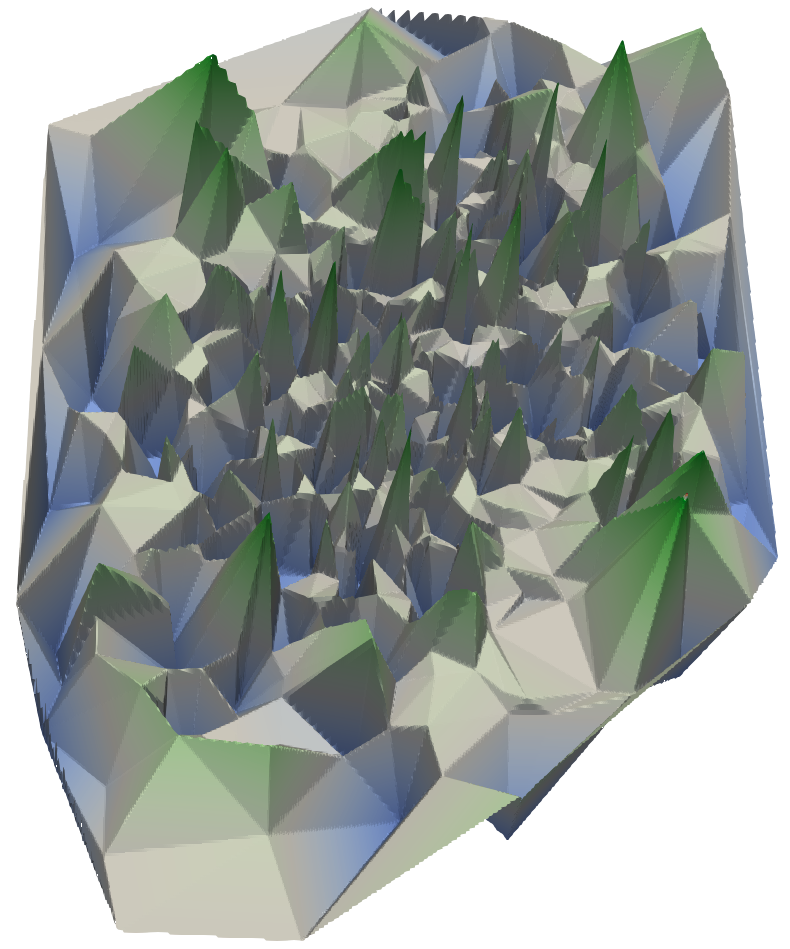
\includegraphics[width=6cm]{figures/coolidge-af-space-sim-vec.png}
}
{

\includegraphics[width=6cm]{figures/tud_logo.eps}
}
\\ \medskip % Picture

\myName \\ % Your name 
%\myDegree \\
%\myDepartment \\
%\myFaculty \\
%\myUni \\ \bigskip

\myTime\ -- \myVersion % Time and version

\vfill

\end{center}
\end{addmargin}

\end{titlepage}

\ifthenelse{\boolean{printversion}}{%
}{
\cleardoublepage
\tableofcontents
}
\cleardoublepage
\vspace*{8cm}
% Sets a PDF bookmark for the dedication
\pdfbookmark{Dedication}{dedication}
\thispagestyle{empty}
\begin{center}
  \Large \emph{Dedicated to ...}
\end{center}
\cleardoublepage
\chapter*{Preamble}
\label{sec:preamble}
\addcontentsline{toc}{chapter}{\nameref{sec:preamble}}
\epigraph{All models are wrong, but some are useful}{George Box (Attributed)}
\section*{Abstract}
\label{sec:abstract}
\addcontentsline{toc}{section}{\nameref{sec:abstract}}
Computer hardware keeps increasing in complexity.
Software design needs to keep up with this.
The right models and abstractions empower developers to leverage the novelties of modern hardware.
This thesis deals primarily with \aclp*{MoC}, as a basis for software design, in a family of methods called software synthesis.

We focus on \aclp*{KPN} and dataflow applications as abstractions, both for programming and for deriving an efficient execution on heterogeneous multicores.
The latter we accomplish by exploring the design space of possible mappings of computation and data to hardware resources.
Mapping algorithms are not at the center of this thesis, however.
Instead, we examine the mathematical structure of the mapping space, leveraging its inherent symmetries or geometric properties to improve mapping methods in general.

This thesis thoroughly explores the process of model-based design, aiming to go beyond the more established software synthesis on dataflow applications.
Starting at the problem of assessing these mehtods through benchmarking, we examine the general goals of benchmarks formally, as well as the role modern machine learning methods play in them.

We explore different established semantics, stretching the limits on \aclp*{KPN}.
We also discuss novel models, like Reactors, which are designed to be a deterministic, adaptive model with time as a first-class citizen.
By investigating abstractions and transformations in the Ohua language for implicit dataflow programming, we also focus on programmability.

The focus of the thesis is in the models and methods, but we evaluate them in diverse use-cases, generally centered around \aclp*{CPS}.
From the 5G telecommunication standard, through the automotive and signal processing domains.
We even go beyond embedded systems and discuss use-cases in \acs*{GPU} programming and microservice-based architectures.
\cleardoublepage
\section*{Publications}
\label{sec:publications}
\addcontentsline{toc}{section}{\nameref{sec:publications}}
Some contents of this thesis, including ideas and some figures, have previously appeared in the following publications: \\ \vspace{1cm}
\printbibliography[heading=none,keyword={contribution}]
\cleardoublepage
\section*{Acknowledgments}
\label{sec:acks}
\addcontentsline{toc}{section}{\nameref{sec:acks}}
First and foremost, I thank my advisor Jeronimo Castrillon.
I consider him to have been both a mentor and a friend during the time I've spent working on this thesis.
His advice shaped my research and this thesis would not exist without his guidance and help.

I also want to thank my current and former colleagues and co-authors at the chair for compiler construction:
Justus Adam, Hasna Bouraoui, Alexander Brauckmann, Sebastian Ertel, Fazal Hameed, Gerald Hempel, Sven Karol, Asif Khan, Robert Khasanov, Nesrine Khouzami, Christian Menard, Norman Rink, Julian Robledo, Lars Schütze and Felix Wittwer.
Thank you for creating a great environment to learn and work together, for countless discussions and insights, for your patience with my insistance on going to Zeltmensa and the great discussions that arose there, and for offering my comradery and friendship. 

I want to thank the students working with me, who've helped me with work, some of whom have become colleagues in the meantime, and from all of whom I've also learned a great deal.
Concretely, thank you, Alexander Brauckmann, Christian Menard, Marcus Rossel, Alexander Thierfelder, Felix Teweleitt and Markus Walter.

During my Ph.D I had the opportunity to visit Andy Pimentel at the University of Amsterdam, where I was warmly received by him, Simon Polstra and the rest of the group.
Thank you for welcoming me and for a fruitful collaboration. I'd also like to thank the HiPEAC project for funding this visit through a collaboration grant.

I also had the opportunity to visit Edward Lee at the University of Califonria at Berkeley. There, Matt Webber and Gil Lederman received me in their office, where I felt very welcome, like any other colleague.
I want to thank both, as well as Marten Lohstroh, all of whom I had great discussions with, and who made my visit at Berkeley extremely fruitful.
A special thank you also goes to Mary Stewart for helping sort out everything there, even to the point of making sure I had something to eat at the group lunches. 
Most of all, I would like to thank Edward Lee for accepting me to visit his group and taking the time to talk with me regularly.
This visit was a pivotal point in my Ph.D. and I really appreciated everything and everyone.
Outside the academic realm, I want to thank Giulia Leggett for making this visit extremely enriching also from a personal point of view.
I also want to thank the German foreign exchange service DAAD and specifically the FIT Weltweit project, as well, the \ac{cfaed} cluster of excellence, for helping me finance this visit.

I also want to thank the rest of my co-authors. Chris Cummins and Hugh Leather for being so open in our collaboration and for their hospitality in Edingburgh. 
To Max Odendahl, for trusting in my abilities while knowing me only on a personal level, and introducing me to the field. Without him, I would never have come to this area of research.
To everyone in the cfead Orchestration path, for sharing a vision with me and constructive retreats.
I also thank Marcus Hähnel and Till Smejkal for a very successful collaboration what started the \acs*{TETRiS} project.
Thanks to Josefine Asmus and Ivo Sbalzarini for collaboration on the work on design centering, which was very insightful.
I also thank Sergio Siccha, for taking our friendly discussions so seriously that we ended up collaborating in the mapping symmetries work.
Thanks also to Robert Wittig for a beachside discussion at Samos that led to a collaboration on the model-based approaches to 5G.

I started this Ph.D. at the \ac{cfaed} cluster of excellence, which provided funding and a great academic environment.
I want to thank everyone at the program office for helping me throughout this time, as well as my thesis advisory committee, Jeronimo Castrillon, Christel Baier and Hermann Härtig.
I also want to thank Conny Okuma for her patience throughout the years with my incomplete formularies and late handing over of documents.
Thanks as well to the German Research Foundation DFG for funding me after \ac{cfaed}.

The final phase of my Ph.D. was mainly funded by the Studienstiftung des deutschen Volkes.
Besides financial support also provided me with an excellent offer of intellectual complementary opportunities.
Thank you for this opportunity, and thanks to Maike Lieser for helping me apply to this scholarship, I am sure I would not have received it without her help.
I also want to thank her for everything else, as she was probably the biggest positive influence in my life during the time of my Ph.D.

I want to thank everyone at TEDxDresden and everyone from animal rights activism for giving me meaningful projects to do with my life besides my research. 
Also to everyone at Bodyworks and Basketball Club Dresden for giving me a constant outlet to find a healthy balance with sports.

Finally, and most importantly, I want to thank my friends and family for being there for me and reminding constantly of all the important and enjoyable aspects of life, besides academics.
To all my friends in and around Dresden, who accompanied me through life these past six years, thank you for making this one of the best times of my life. 
To my friends back in Aachen, San Salvador and spread throughout the rest of the world, thanks for being a constant source of love and friendship that has kept me grounded.
I won't list everyone who has made my life better these last six years and whom I consider a friend, I'm sure they know who they are, and I thank each and every one.

I would certainly not be who I am, and this thesis would not be possible, without the tremendous support from my family. 
My cousins, uncles and (great) aunts, my two big sisters, thank you everyone for always being there for me. 
Especially my little sister Ute, who's accompanied me a large part of my time here in Dresden, being a constant source of support and inspiration.
My father made me be curious and think critically since I was a kid, and coupled this inspiration with unconditional love, which I am certain was an indispensable for me to write this thesis.
My mother made me be social and empathic, and made sure I became a well-rounded person.
Her constant support and openness made me always do what interested me, and I am certain this thesis would never have happened without her.
Thank all of you for everything!
\cleardoublepage
\ifthenelse{\boolean{printversion}}{
\cleardoublepage
\tableofcontents
}{}
\pagenumbering{arabic} 
\chapter{Introduction}
The last two decades have firmly established the multicore era. Modern computing systems are almost universally composed of multiple logical cores, and there is a clear trend of increasing both the number and the heterogeneity of these cores. This increasing complexity brings about an increasing challenge in taming it. Inspired by hardware design flows, a family of methods called software synthesis aims to bridge the ensuing (software) productivity gap by integrating knowledge of the application and target multicore architecture into the compilation process. The aim of this thesis is to identify and exploit structures in the different parts of this process to improve the methods.

\begin{figure}[h]
	\centering
   \resizebox{0.55\textwidth}{!}{\begin{tikzpicture}
\draw (0,0) rectangle (5,5);
\draw (2.5,2.5) node {Placeholder};
\end{tikzpicture}
}
	\caption{The multicore era.} %something like: https://www.karlrupp.net/wp-content/uploads/2015/06/40-years-processor-trend.png
	\label{fig:multicore_era}
\end{figure}


%Multicore Era
Both the execution frequency and the closely intertwined single-core processing speed of computing systems increased exponentially up until the early 2000s (cf. Figure~\ref{fig:multicore_era}), an empirical fact observed by Gordon Moore in 1965~\cite{moore}. A programmer writing a piece of C code in the early 1970s would automatically benefit from the increasing processing speeds. By recompiling her code for a processor $10 \times$ faster, she could expect her code also to run about $10 \times$ as fast.% Do I want to make this concrete (with Processor names?)

Since the early 2000s, however, while tranistor size continue to decrease, the exponential frequency scaling has stopped. Instead, hardware designers resorted to develop microchips composed of multiple logical cores that can execute in parallel. Additionally, since different use-cases benefit from different computing core architectures, the inclusion of multiple chips has paved the way for heterogeneity. This has resulted in a multicore era of computing. Contemportary systems almost ubiqutiously consist of multicore chips, in many cases heterogeneous, which tremendously increases the system complexity. The trend is clear, the number of cores, heterogeneity and overall system complexity will only continue to increase.

% Software Productivity gap: Software Synthesis
Nowadays thus, a programmer writing a piece of (sequential) C code in the early 2000s cannot expect anywhere near a $100$-fold increase in performance today when she uses a microchip with $100 \times$ the number of transistors.
At least not without fundamentally restructuring her code to exploit parallelism.
More generally, the burden of maximally exploiting the hardware capabilities falls on the compiler and programmer, instead of coming automatically with the improvements in hardware.
This includes difficult problems like expressing parallelism and dividing tasks between different physical cores. %todo: perhaps discuss expressing parallelism

Software synthesis refers to a family of methods deviced precisely to help with this burden of fully exploiting the capabilities of modern multicores. At the core of these methods lies a shift in the programming model. Instead of the de-facto sequential, shared-memory model, programmers express the code in diverse \acp{MoC}. These models expose the structure of the computation in ways that permit a compiler to reason about its parallel execution, even in the prescence of heterogeneous hardware. Aided by abstract models of the target archicecture, we can design compilers for multicore systems that devise execution strategies specialized to the target architecture and applications. This can be realized for example by finding efficient mappings, i.e. allocations of computational and communication resources to the different parts of an application.

% Exploiting Structure in Dataflow Software Synthesis: Part I
The software synthesis process is centered around multiple formal constructs modeling the application and architectures, as well as decisions of the execution of the former on the latter, like mappings.
These are all rich in (mathematical) structure. Architectures for example, even heterogeneous ones, exhibit a great deal of symmetry. Similarly, the space of mappings has locality properties, where some mappings are similar whereas others are to others. In this thesis we aim to identify and exploit these structures in different ways. The first part of this thesis does this with a concrete software synthesis flow, which models applications as \acp{KPN} and finds mappings of these to heterogeneous systems.

% Other improvements changing the methods (Part II)
While Software Synthesis refers to a family of methods, each concrete method has a corresponding choice of abstractions it uses. Instead of exploiting the structure of the given abstractions, in the second part of this thesis we explore ways in which we can improve upon software synthesis methods by changing the structure we use: be it the semantics of the model of computation, implicit language structures or even the benchmarks we evaluate to asses our methods.

\begin{figure}[h]
	\centering
   \resizebox{0.55\textwidth}{!}{\begin{tikzpicture}
\draw (0,0) rectangle (5,5);
\draw (2.5,2.5) node {Placeholder};
\end{tikzpicture}
}
	\caption{A placeholder picture.}
	\label{fig:placeholder}
\end{figure}

\begin{figure}[h]
	\centering
   \resizebox{0.55\textwidth}{!}{\input{generated/placeholder_plot.tex}}
	\caption{A placeholder plot.}
	\label{fig:placeholder}
\end{figure}

A placeholder reference\cite{goens_multiprog18}.


%The first part of this thesis deals with improving dataflow-based software synthesis. Software synthesis refers to a series of related methods, with the common goal of efficiently deploying software on a specific hardware architecture. While the aim of this thesis is to analyze structures and present methods that are general to software synthesis as a whole, in practice we will always work with concrete design flows. The first part of the thesis thus deals with design flows based around mapping dataflow applications to heterogeneous \acp{MPSoC}, on the example of a flow based on \acp{KPN}, but including other models of computation. For this flow we will investigate multiple structural properties of the applications, architectures and mappings and show how to exploit these. Symmetries of applications and architectures result in symmetries of mappings, which can be exploited both for \ac{DSE} and at runtime. The spatial structure of the mappings and the way mappings are represented can also be leveraged in different mapping algorithms, like those based bio-inspired design centering and genetic algorithms. Finally, we discuss the structure of data allocation in memory.
\chapter{Mapping \acsp{KPN} to Heterogenous \acsp{MPSoC}}
\label{chap:mapping}
The central concept in software synthesis as studied in this chapter is the concept of a \emph{mapping}\index{mapping}.
In this chapter we will consider mappings and their general mathematical structure, whereas Chapter~\ref{chap:mapping_applications} will deal with concrete applications of this structure to improve different aspects of the software synthesis process.

Intuitively, a mapping distributes a computation (and its corresponding data) to physical resources in a specific hardware.
This can be done dynamically\index{mapping!dynamic}, for example as is the case with tasks scheduled by \acs{CFS} in a modern Linux-based operating system.
Conversely, a \emph{static} mapping\index{mapping!static} as the one depicted in Figure~\ref{fig:mapping_idea} maps the computation and data statically, usually at compile time, to specific hardware resources.
Finally, there are also \emph{hybrid} mappings \index{mapping!hybrid}, in which partial decisions are taken statically, but the final decision happens at compile-time. 

In software synthesis we strive to derive an efficient execution from a computation expressed in an abstract model to a concrete architecture.
In order to understand software synthesis, thus, we first need to understand the underlying models of computation.
Closely related to these concurrent models of computation are execution traces, which capture a concrete execution for some input.
However, going from such abstract models to a concrete execution also requires an understanding of the target hardware architecture.
The relationship between the two can be captured in a mapping.
This chapter considers all of these aspects with their corresponding models, and the relationship between them.
It is the central piece of background theory required for the methods presented in this thesis.

\subsection{Kahn Process Networks}

The flow we investigate in Part I is based on the \ac{MoC} of \acfp{KPN}.
In this section we introduce this model, or rather, its most common implementation with blocking-read semantics~\cite{kahn_macqueen} .
In Part II, specifically in Chapter~\ref{chap:mocs} we will discuss the original formal semantics~\cite{kahn74} and how they differ to those introduce here.
We also discuss other models of computation and how they relate to each other.

We can think of a \ac{KPN} as a computation distributed among different \emph{processes}\index{KPN ! process} (originally derived from coroutines).
Each of these processes executes sequentially and is Turing complete. However, the processes share no memory, they have memories local only to themselves.
They communicate between each other using \emph{channels}\index{KPN ! channel}, which work as unbounded \acs{FIFO} buffers. 
Processes have sets of outgoing and incoming channels.
As an instruction, any process can write to one of its outgoing channels or read from one of its incoming channels.
They do so in discrete tokens of data.

The original language~\cite{kahn_macqueen} was proposed as an extension of POP-2, which is pretty dated and has fallen out of use today.
Instead of this language, we will consider a more modern incarnation, \ac{CPN}, which extends the C programming language~\cite{cpn}\index{CPN}.
We do so by looking at the example from Listing~\ref{listing:fft_cpn}. 
The listing shows a very simplified process that applies an \acs{FFT} it the data in its incoming channel and outputs it to an outgoing channel.
Processes in \ac{CPN} are instantiated from process templates, similar to classes and objects in object-oriented languages.


\begin{listing}
\begin{minted}{C}
__PNkpn fft_templ
    __PNin(param_t param, time_coef[N])
    __PNout(fp_complex freq_coef[N]){
  int i, loop_count;
  __PNin(param){
    loop_count = param.loop_count;
  }
  for (i = 0; i < loop_cnt; i++)
    __PNin(time_coef) __PNout(freq_coef){
      fft(time_coef, freq_coef);
    }
}
\end{minted}
\caption{An \ac{FFT} implemented as a \ac{KPN} process in \ac{CPN}}
\label{listing:fft_cpn}
\end{listing}


The communication is asynchronous: 
When a process writes to an outgoing channel, the data is buffered in the channel until it is read, and the process continuous to execute.
If a process reads from a channel, it receives the oldest token buffered in the channel.
If there are no tokens, execution blocks until such a token is written to a channel - hence the name, blocking-read semantics.
A channels can be the outgoing channel of at most one process (it should also be so for at least one process, otherwise the channel is useless).
On the other hand, if a channel is an incoming channel to multiple processes, all tokens are copied for each of those processes.
Hence, all processes will see the exact same incoming stream of tokens from a shared channel, instead of splitting them up.

Let us consider the \acs{FFT} process from Listing~\ref{listing:fft_cpn} and combine it with other processes into a full application.
Listing~\ref{listing:audio_filter} describes a simplified algorithm for a low-pass filter on a stereo sound file, using this \acs{FFT} process.
We also omit the templates and channel declarations in this simplified listing.
The \texttt{src} process reads the stereo file, splits it into two channels and sends the sound in blocks of a determined length as tokens.
These files are then transformed from the time domain to the frequency domain using a \acf{FFT}, filtered and transformed back to the time domain.
A sink channel gathers the filtered blocks from both channels, left and right, and combines them again into a stereo sound file that it can store.

\begin{listing}
\begin{minted}{C}
__PNprocess src = src_templ
  __PNout(param_chan, src_l, src_r);
__PNprocess fft_l = fft_templ
  __PNin(param_chan, src_l)
  __PNout(fft_coef_l);
__PNprocess filter_l = filter_templ
  __PNin(param_chan, fft_coef_l)
  __PNout(filtered_coef_l);
__PNprocess ifft_l = ifft_templ
  __PNin(param_chan, filtered_coef_l)
  __PNout(sink_l);
__PNprocess fft_r = fft_templ
  __PNin(param_chan, src_r)
  __PNout(fft_coef_r);
__PNprocess filter_r = filter_templ
  __PNin(param_chan, fft_coef_r)
  __PNout(filtered_coef_r);
__PNprocess ifft_r = ifft_templ
  __PNin(param_chan, filtered_coef_r)
  __PNout(sink_r);
__PNprocess sink = sink_templ
  __PNin(param_chan, sink_l, sink_r);
\end{minted}
\caption{An audio filter \ac{KPN} application in \ac{CPN}}
\label{listing:audio_filter}
\end{listing}

The data flow in the example of Listing~\ref{listing:audio_filter} is very structured: it goes from the source, split over both channels, through the filter, back to the sink.
This structure can easily be visualized in a graph, like in Figure~\ref{fig:audio_filter_graph}.
More generally, we can think of any \ac{KPN} application as a directed graph $K = (T,C)$, where the nodes $T$ represent the processes\footnote{the notation comes from $T$ for tasks}, and the edges $C$, the channels.
This works even when a channel is an incoming channel for multiple processes.
In that case, we can split it into multiple edges from the process it is going from, to each of the target channels.
We can do so without loss of generality since these are the semantics of such channels. 
We call this graph the \emph{\ac{KPN} graph}\index{KPN ! graph}.

\begin{figure}[h]
	\centering
   \resizebox{0.9\textwidth}{!}{\begin{tikzpicture}
\draw (0,0) rectangle (5,5);
\draw (2.5,2.5) node {Placeholder};
\end{tikzpicture}
}
   \caption{The audio filter application as a \ac{KPN} graph}
	\label{fig:audio_filter_graph}
\end{figure}

\subsection{Execution Traces}

Kahn Process Networks with mathematical semantics~\cite{kahn74}, in the sense of Scott~\cite{scott1970}, abstract away the concrete implementation of individual steps in a computation.
Even so, the execution of a computation can be thought of as a series of steps or partial computations that eventually yield the final result.
These series, which is commonly referred to as execution trace, can be captured as a sequence of steps, e.g. as the element of a Scott Domain\footnote{this will be discuss more in-depth in Chapter~\ref{chap:mocs}}. 
Abstract computations, modeled as Scott-continuous functions, can can make computations of arbitrary length.
This is modeled by (countably) infinite sequences in $D^\omega \setminus D^*$.
A concrete execution, on the other hand, always has a finite length.
It always resides in $D^*$.
For a (Scott-continuous) function, this sequence can be modeled as a finite string in the computation domain.

In a concurrent execution, multiple entities concurrently execute steps.
As modeled by Kahn, these entities all implement individual (Scott-continuous) functions.
As such, there is not a unique series of steps that can be said to be the execution trace of the computation.
To see this, consider the following example:
\begin{ex}
  Todo
\end{ex}

TODO: discuss example

In the distributed case thus, the execution traces are in fact equivalence classes of strings.
We define this more formally, following~\cite{mazurkiewicz1995introduction}, the first chapter of~\cite{diekert1995book}.
Let $D$ be a finite set, like an alphabet $\Sigma$ or data type $D = \Cup_{i \in \mathcal{I}} D_i$ be a data type for a \ac{KPN}.
Let $\Delta$ be a symmetric, reflexive relation on $D$, which we call a dependency\index{dependency}.
This means that if $(a,b) \in \Delta$, we have $(b,a) \in \Delta$ and also $(a,a) \in Delta$ for all $a \in D$. 
With $\Delta$ we define an additional relation in $D$, namely $I := (D \times D) \setminus \Delta$.
We call $I$ the induced independency\index{independency}. 
We define an equivalence relation $\sim_I$ on the monoid $D^*$ (with respect to concatenation) as follows:
We require for $a,b \in I$ then $ab \sim_I ba$. The relation $\sim_I$ is defined as the least congruence that satisfies this requirement.
Note that a congruence is an equivalence relation that respects the algebraic structure, in this case the monoid structure of the concatenation operation.
We call the equivalence classes of $D^*/{\sim_I}$ traces. 
By definition, the concatenation operation on $D^*$ factors over the equivalence relation $\sim_I$,
and thus $D^*/{\sim_I}$ defines a monoid (with identity element $[\epsilon]_{\sim_i}$, where $\epsilon \in D^*$ is the empty string).
We call this the Trace Monoid\index{trace monoid}, $T(D)$.
We care about the algebraic structure of a monoid since it is central to the definition of Scott-continuity.

\begin{ex}
  Todo (based on example above)
\end{ex}

There are two additional equivalent definitions of this monoid as histories and dependence graphs.
We present histories here, as they are easier for the intuition.
Instead of a single alphabet (or set of types) $D$, we have a finite set of alphabets $D := (D_i), i \in \mathcal{I}$, where $\mathcal{I}$ is a finite index set.
We can think of the indices as corresponding to the processes or actors in the system, and the alphabets $D_i$ to the alphabets of these individual entities.
If we think of the individual entities as computing some (Scott-continuous) function, their execution trace will be a unique string $a_i \in D_i^*$ (recall that concrete executions are finite).
Since, in general, these entities do not compute independently, they have common synchronization points.
These synchronization points are abstractly modeled in the computation alphabet by mutual elements in $D_i \cap D_j$ for two entities $i,j \in \mathcal{I}$.
We can define a monoid, the product monoid~\index{product monoid} $P(D)$, by component-wise concatenation of the strings: $(a_i)_i (b_i)_i = (a_ib_i)_i$ for all $i \in \mathcal{I}$.
However, not every such a string product can be the history of a system.
The synchronization points of different subsystems should be consistent with each other. Consider the following example:
\begin{ex}
  \label{ex:inconsistency_history}
TODO: slight variation that shows an element of $P(D) \setminus H(D)$
\end{ex}
To avoid this, we want to ensure histories are consistent. For this, we define elementary histories~\index{elementary history} as follows:
For any $a in \Cup_{i \in \mathbb{I}} D_i$, the elementary history of $a$ is the tuple $(a_i)_{i \in \mathbb{I}}$, with $a_i = \left\{ \begin{array}{ll} a, & \text{ if } a \in D_i, \\ \epsilon, & \text{ otherwise. }\end{array}\right.$
Again, $\epsilon$ represents the empty string.
The monoid generated by all elementary histories for elements in $\Cup_{i \in \mathbb{I}} D_i$ is called the history monoid $H(D)$, and is a submonoid of $P(D)$.
If we examine the definition, it is not difficult to convince ourselves that these are precisely the histories which avoid inconsistencies like those of Example~\ref{ex:inconsistency_history}.

\begin{ex}
  Todo (based on example above)
\end{ex}

We can go from a trace to a history by the morphism $\pi: T(\Cup_{i \in \mathcal{I}}) \rightarrow H(D), a \mapsto (\pi_i(a))_i, i \in \mathcal{I}$, where $\pi_i$ is the projection $\Cup_{i \in \mathcal{I}}D_i \rightarrow D_i$.
Here, for the trace monoid $T(D)$ we define the dependencies to be $\Cup_{i \in \mathcal{I}}D_i \times D_i$. 
This is not just a morphism, but in fact an isomorphism: See Theorem 1.5.4 of~\cite{mazurkiewicz1995introduction}.
Thus, the two concepts are equivalent.
For the rest of this thesis we will use the terms traces and histories interchangeably.


Traces, and equivalently histories, can be used to describe the concrete computations in concurrent systems like those described by a \ac{KPN}.
They are also well-suited (and well-suited) to model these systems in the context of process calculi, like \ac{CSP}.
However, an important observation is the converse: a concrete execution of a \ac{KPN} is determined uniquely by its history.
Moreover, any concrete implementation of the \ac{KPN} realizing the same execution will have the same history: the history is an invariant of the abstract execution model.
It captures the concurrent essence of the concrete computation.

\subsection{Architecture Models}
Discuss ad-hoc models, \cite{pelcat2015models}. Go in-depth on architecture graph (and topology graph).

\subsection{The Mapping Problem}
A lot more...\cite{singh2013mapping} \cite{marwedel2011mapping}

\subsection{Limits of the Model}
Only discuss briefly here.

\section{Simulating Mappings}
\label{sec:simulating_mappings}
Simulations are extremely important for analyzing an application's performance, or more generally, its behavior.
As described in Section~\ref{sec:arch_models}, there are multiple levels of detail in which to model and, consequently, simulate, an architecture and its execution.
For investigating the mapping problem in software synthesis, higher-level simulations are preferable for multiple reasons.
First and foremost, higher-level simulations are faster.
If a meta-heuristic iteratively evaluates dozens, hundreds or even thousands of mappings to find a near-optimal one, it greatly benefits from the fast evaluation time associated with a higher-level simulation.

Higher levels of abstraction come with a trade-off, accuracy of the simulation suffers in exchange for the simpler models and faster simulation times.
Let $\tilde \Theta$ be the approximation of $\Theta$ from the simulation. A loss in accuracy means that $| \Theta(m) - \tilde \Theta(m)|$ becomes larger.
However, depending on the use-case and mapping objective $\Theta$, this loss in simulation accuracy might not necessarily affect the quality software synthesis results.
Suppose that the objective $\Theta$ represents execution time or energy consumption, and the goal of the software synthesis is just a best-effort minimization of $\Theta$ (with no additional constraints, i.e. $C \equiv \operatorname{True}$).
Then the accuracy of the simulation is not important, only its fidelity.
If $\Theta(m_1) < \Theta(m_2)$ we want the result of the simulation to reflect this, $\tilde \Theta(m_1) < \tilde \Theta(m_2)$.
As long as this is the case, we don't care about the actual value of $| \Theta(m_i) - \tilde \Theta(m_i)|$, since in this case the exploration will still find the minimum.
The fidelity of the simulation is a measure of how often this is true.
On the other hand, if the application is a real-time application, then the truth value of $C$ will depend on the accuracy of the simulation.
Here, the accuracy of the simulation is much more important.

This chapter describes the simulation aspects which pertain the models of computation and the practical tooling we will use.
Nuanced simulation details and advanced techniques are beyond the scope of this thesis.

\subsection{Simulating the Execution of Kahn Process Networks}

The behavior of a system plays a central role in simulation. A deterministic model should yield deterministic simulation results.
Non-determinism, when present, should also be captured by the models and reflected by the simulations.

The behavior of systems is commonly captured in execution traces, which simply record the behavior of different entities (e.g. processes or actors) at different timepoints.
This can be formally captured in a monoid structure of (Mazurkiewicz) traces or, equivalently, histories~\cite{diekert1995book}.
Traces are useful to understand the behavior of systems~\cite{vampir} and are common in many domains.
However, for systems that are non-deterministic, (by definition) the behavior of the system does not only depend on the input.
This can make designing~\cite{lee2006problem} and debugging~\cite{murillo_debugging} particularly difficult.
In cyber-physical-sytems or, more generally, reactive systems in the sense of Harel and Pnueli~\cite{harel_pnueli_reactive}, input from the physical world might come in a non-deterministic fashion.
The problem of capturing the behavior of such a system is even more complex when the system is distributed~\cite{shaver_phdthesis}. 

Kahn Process Networks are deterministic, as are all the dataflow models that can be embedded as KPNs.
This means that the behavior of a KPN application depends only on the input to the network.
In particular, it does not on the mapping and scheduling or related execution details.
Thus, their behavior can be captured by a (Mazurkiewicz) trace.
This permits to re-create their behavior in a fashion that is independent of the mapping~\cite{find_proper_references}.
By ``replaying'' the trace, i.e. simulating the execution of a process for every input in the trace, a discrete-event simulator can successfully simulate the execution of a KPN, since the token sequence is guaranteed to be identical given identical inputs.
In particular, this allows us to do design-space exploration.

A discrete-event simulation of a KPN application thus requires behavior traces. It also needs to model the execution and communication times.
Modeling execution times from a trace is simple, with a crucial assumption: if the execution times for a trace event only depend on the PE type.
This assumption won't hold always hold, e.g. when the instruction cache is flushed due to scheduling decisions, or due to unpredictability from the \ac{OS}.
Note that data caches are modeled as part of the communication between processes.
However, in most cases this assumption is a good approximation, it is normal to expect that the same code executing on the same data and the same \ac{ISA} will usually require the same amount of time.

Modeling communication is more complicated, as it depends on the memory subsystem. In general, the communication costs of sending a KPN token depend on multiple factors, like the size of the token, contention in the memory subsystem (and correspondingly methods of arbitration, routing in the case of a \ac{NoC}, etc), or the API and protocol being used.
For the simulations in this thesis, we use a model based on annotations of the architecture graph $A$. These annotations are functions that calculate the time cost of communicating data, as a function of its size.
In this way, we model both the latency and bandwidth of the communication.
We use a split-cost communication model to assign costs to sending and receiving data~\cite{odendahl2013split}.
This separation can be used to simulate based on traces, as described above, since we can then compute the cost of communication for both the sending and receiving processes.

When dealing with \ac{NoC}-based architectures, this model is not as accurate.
Communication over a \ac{NoC} depends also on the routers and links along the path, including the routing algorithms.
We extended the split-cost communication model to account for these issues in~\cite{menard_norcas16}.
The idea is to add a third term to account for the network, in addition to the consumer and producer costs. 
This third term can account for the routing and the topology of the network while maintaining an analytic model which is cheap to evaluate in a high-level simulation.

Simulation is essential for software synthesis, yet it is not the focus of this thesis. As such, we will only discuss the main idea behind the analytic models and their relationship to a fast simulation of \ac{NoC}-based architectures.
The main contribution of~\cite{menard_norcas16}, with a concrete model for the Tomahawk~2 architecture~\cite{tomahawk2} and the corresponding evaluation comparing to the SystemC-based simulator Noxim~\cite{noxim} are due to my coauthors and beyond the scope of this thesis.


\section{The \mocasin tool}
\label{sec:mocasin}


In this thesis we will use \mocasin, a tool for the Model-of-Computation-based Analysis and Simulation of applications~\cite{menard_rapido21}.
This tool, formerly known as \texttt{pykpn}~\cite{goens_mcsoc18}, has been developed as part of a collaborative effort between multiple researchers at the Chair for Compiler Construction at TU Dresden.
While the tool itself is a joint contribution with the coauthors of~\cite{menard_rapido21}, many concepts introduced in this thesis have been implemented and tested using \mocasin.
As such, this section will explain the tool in-depth, to enable the description of the different implementations of contributions from this thesis implemented in \mocasin.

\begin{figure}[h]
	\centering
   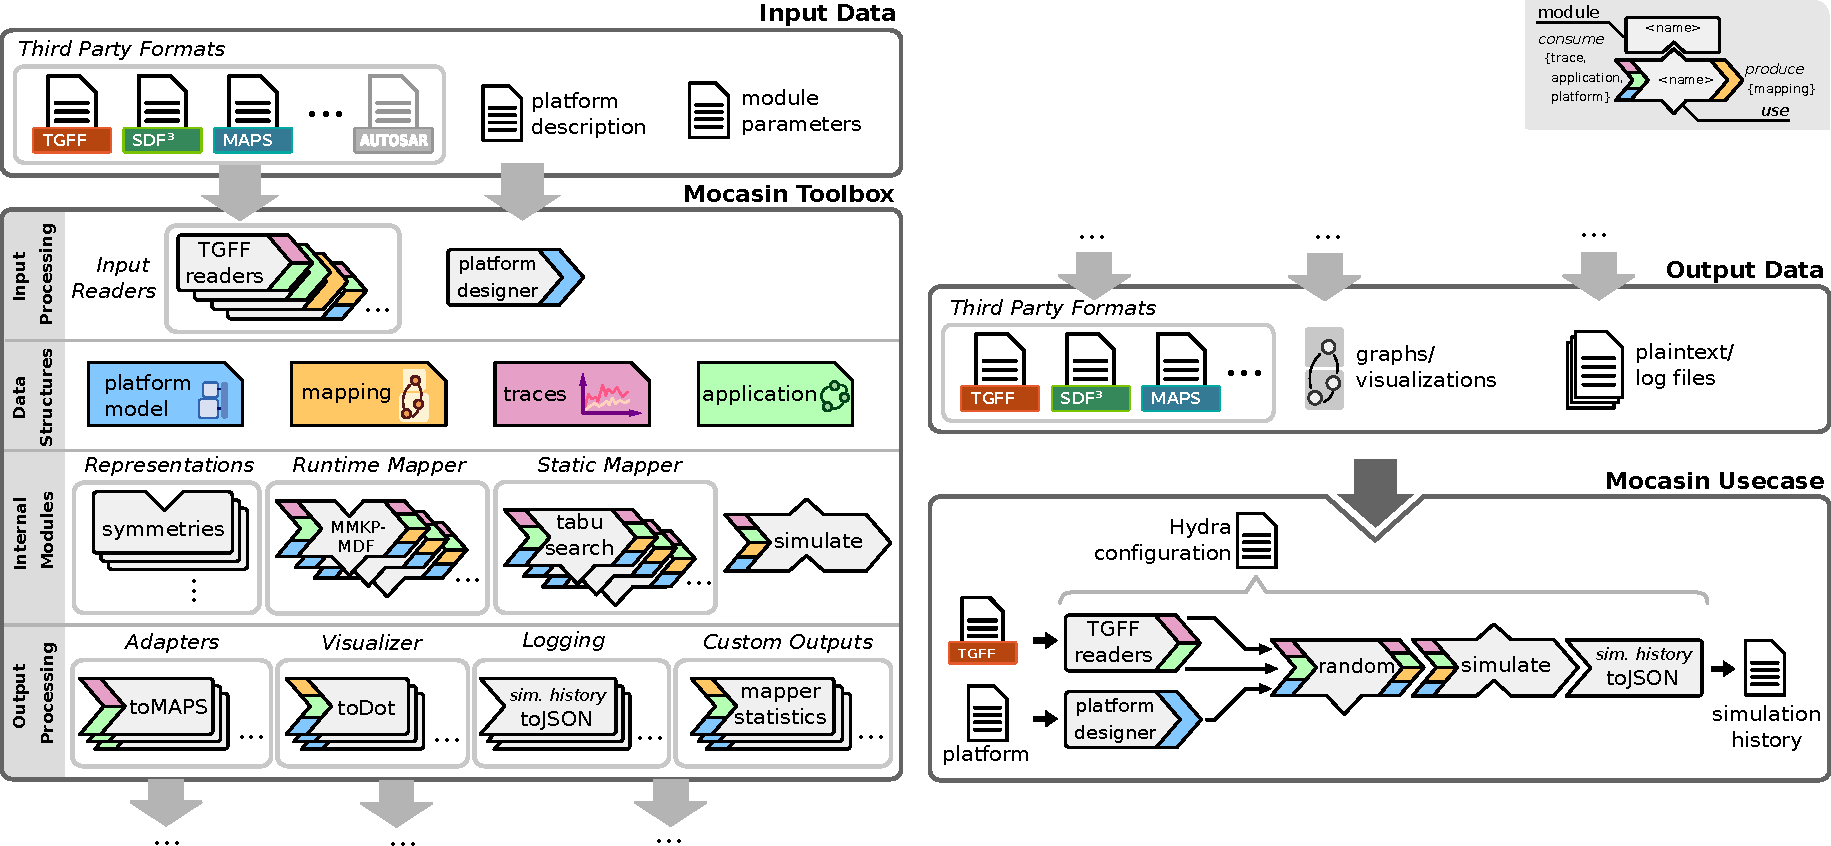
\includegraphics[width=0.95\textwidth]{figures/mocasin.pdf}
	\caption{The \mocasin architecture. Adapted from \cite{menard_rapido21} (Figure~2).}
	\label{fig:mocasin_arch}
\end{figure}


Figure~\ref{fig:mocasin_arch} depicts the basic flow of \mocasin.
It can be understood as a tool for rapid prototyping of prototyping tools.
Multiple dataflow \acp{MoC} are supported by \mocasin, like \ac{SDF} or task graphs.
These models, among others, can be seen as specializations of \ac{KPN}~\cite{lee1995dataflow} and will be discussed more in-depth in Chapter~\ref{chap:mocs}.
The \mocasin architecture is composed of multiple modules that can be combined to create a specific tool (e.g. for mapping or simulation). 

In general, simulating a KPN requires four inputs, as explained in Section~\ref{sec:mappings_background}: the KPN graph, a platform description, execution traces and a mapping.
\mocasin has data internal structures for these four inputs that reflect the models as explained in Sections~\ref{sec:kpn_basic,sec:traces,sec:arch_models,sec:mapping_problem}.
The tool boasts multiple readers to generate the internal data structures from established formats like \texttt{tgff}, \texttt{sdf3} or the \texttt{MAPS} formats.
Instead of a concrete trace, \mocasin expects a trace generator, which can generate the trace on the fly: this is useful e.g. for non-deterministic models computation, but for KPNs the two are equivalent.
The \ac{KPN} trace generator, for example, simply reads the trace from a file.
A mapping, while required for simulation, does not need to be provided: it can be calculated in a design-space exploration.
This is not surprising, since a significant part of this thesis concerns itself with finding good mappings efficiently.

A central part of \mocasin is a discrete-event simulator that uses the principles outlined above to simulate KPN applications based on their traces (as well as other models of computation).
We will not dwell on the design of the \texttt{simulate} module since it goes beyond the contribution and scope of this thesis.
In the following, we will describe some other central modules of \mocasin. 


\subsubsection{platform designer}

\begin{listing}
\begin{minted}[]{python}
designer = PlatformDesigner(self)
designer.setSchedulingPolicy('FIFO', 1000)
designer.newElement("exynos5422")
# cluster 0 with l2 cache
designer.addPeClusterForProcessor("cluster_a7", processor_0, num_little)
# Add L1/L2 caches
designer.addCacheForPEs("cluster_a7", 1, 0, 8.0, float('inf'),
                        frequencyDomain=1400000000.0, name='L1_A7')
designer.addCommunicationResource("L2_A7", ["cluster_a7"], 250, 250,
                                  float('inf'), float('inf'),
                                  frequencyDomain=1400000000.0)
# cluster 1, with l2 cache
designer.addPeClusterForProcessor("cluster_a15", processor_1, num_big)
# Add L1/L2 caches
designer.addCacheForPEs("cluster_a15", 1, 4, 8.0, 8.0,
                        frequencyDomain=2000000000.0, name='L1_A15')
designer.addCommunicationResource("L2_A15", ["cluster_a15"], 250, 250,
                                  float('inf'), float('inf'),
                                  frequencyDomain=2000000000.0)
# RAM connecting all clusters
designer.addCommunicationResource("DRAM", ["cluster_a7", "cluster_a15"],
                                  120, 120, 8.0, 8.0,
                                  frequencyDomain=933000000.0)
designer.finishElement()
\end{minted}
\caption{The Odroid-XU4 Platform with the Platform Designer}
\label{listing:designer_odroid}
\end{listing}

\subsubsection{mappers}

\subsubsection{configuration}

Using Hydra~\ref{yadan2019-hydra}.

\subsubsection{contribution}


\begin{figure}[h]
	\centering
   \resizebox{0.95\textwidth}{!}{% Define block styles
\tikzstyle{mio} = [rectangle, rounded corners, draw, fill=green!20, %legend: possible "IP leak"
    text width=7em, text centered, minimum height=4em]
\tikzstyle{block} = [rectangle, draw, fill=blue!20, 
    text width=7em, text centered, rounded corners, minimum height=4em]
\tikzstyle{required} = [draw, ->]
\tikzstyle{possible} = [draw, dashed, ->]
\tikzstyle{interaction} = [thick, <->, draw, color=red!70]
\tikzstyle{data} = [rectangle, rounded corners, draw, fill=teal!20, text width=7em, text centered,  minimum height=4em]

\begin{tikzpicture}[node distance = 4em]
    % inputs/readers
    \node [block ] (tgff) {tgff readers};
    \node [block, below=of tgff ] (sdf3) {sdf$^3$ readers};
    \node [block, below=of sdf3] (slx) {SLX readers};

    %data
    \node [data, right=of tgff] (traces) {traces};
    \node [data, below=of traces] (app) {application (e.g. KPN)};
    \node [data, below=of app] (mapping) {mapping};
    \node [data, below=of mapping] (platform) {platform model};

    \node [block, left=of platform] (platformdes) {platform designer};

    %modules
    \node [block, right=of mapping] (mappers) {mappers};
    \node [block, right=of app] (simulate) {simulate};
    \node [mio, above=of simulate] (tetris) {runtime managers (Section~\ref{sec:tetris}) };
    \node [mio, right=of mappers] (logic) {logic language manager (Section~\ref{sec:logic_language})};
    \node [mio, below=of mappers] (representations) {representations (Chapter~\ref{chap:mapping_structures})};
    \node [mio, above=of logic, align=center] (dc) {design centering \\ (Section~\ref{sec:design_centering})};


    %edges
    \path [possible] (slx) -- (traces);
    \path [possible] (slx) -- (app);
    \path [possible] (slx) -- (platform);
    \path [possible] (slx) -- (mapping);

    \path [possible] (tgff) -- (traces);
    \path [possible] (tgff) -- (app);
    \path [possible] (sdf3) -- (traces);
    \path [possible] (sdf3) -- (app);

    \path [possible] (platformdes) -- (platform);

    \path [required] (traces) -- (mappers);
    \path [required] (app) -- (mappers);
    \path [required] (platform) -- (mappers);
    \path [required] (mappers) -- (mapping);



    \path [required] (traces) -- (simulate);
    \path [required] (app) -- (simulate);
    \path [required] (platform) -- (simulate);
    \path [required] (mapping) -- (simulate);

    %interactions
    \path [interaction] (mappers) -- (logic);
    \path [interaction] (mappers) -- (representations);
    \path [interaction] (simulate) -- (tetris);
    \path [interaction] (simulate) -- (mappers);
    \path [interaction] (simulate) -- (dc);

    \matrix [draw=black,fill=gray!10,above=13em of traces.north west, anchor=north west] {
      \node[data, rounded corners=0, text width=1em, minimum height=1em] {}; & \node[] {data structure};\\
      \node[block, rounded corners=0, text width=1em, minimum height=1em] {}; & \node[] {module};\\
      \node[mio, rounded corners=0, text width=1em, minimum height=1em] {}; & \node[] {module with contributions from this thesis};\\
      \draw[possible] (0,-0.2) -- (0.4,-0.2); & \node[] {optional input data};\\
      \draw[required] (0,-0.2) -- (0.4,-0.2); & \node[] {internal data depencency};\\
      \draw[interaction] (0,-0.2) -- (0.4,-0.2); & \node[] {interaction between modules};\\
      % \node[fill=black,draw,circle,inner sep=2pt,outer sep=0pt] (m) at (0,0){};
      % \draw (m) -- +(0,0.4); & \node[legendtext]{Mandatory}; & 
 %   \filldraw[fill=white,draw=black] (0,0.2) -- ++(225:0.2) arc[start angle=225,end angle=315,radius=0.2]; 
 % \draw (0,0.2) ++(225:0.5) -- (0,0.2) -- ++(315:0.5);& \node[legendtext]{Alternative}; \\
 %  \node[fill=white,draw=black,circle,inner sep=2pt,outer sep=0pt] (o) at (0,0){}; \draw (m) -- +(0,0.4); & \node[legendtext]{Optional}; & 
 %  \draw (0,0.2) ++(225:0.5) -- (0,0.2) -- ++(315:0.5);
 %  \filldraw[black] (0,0.2) -- ++(225:0.2) arc[start angle=225,end angle=315,radius=0.2]; & \node[legendtext]{Or}; 
\\
};
\end{tikzpicture}
}
	\caption{Simulating KPN Applications in \mocasin. TODO: this figure should actually come later}
	\label{fig:mocasin_kpn_simulation}
\end{figure}

\chapter{Benchmarking}
\label{chap:benchmarking}
The methods we will discuss in this thesis are ultimately about improving the performance of software. 
We need benchmarks to assess the performance of software, and consequently to assess if the performance improves.
Benchmarks are essential for the research and development of compilers and programming languages~\cite{hall_compiler_research}, as well as hardware architectures or runtime systems.
In this context, benchmarks are generally understood to be collections of programs with particular properties.
Mostly, they cover a range of behaviors that are typical of, and important for programs in a particular domain.
This description, however, can mean several different things.
% In this section, we formally define different classes of benchmarks and argue how they might be desirable in different scenarios.
In this chapter, we formally define different types of benchmarks and use them to classify different use cases.
We then proceed to discuss concrete \ac{KPN} and task-graph benchmarks for software synthesis, as well as benchmark generation strategies both with random graph models and machine learning.

\begin{figure}[h]
	\centering
	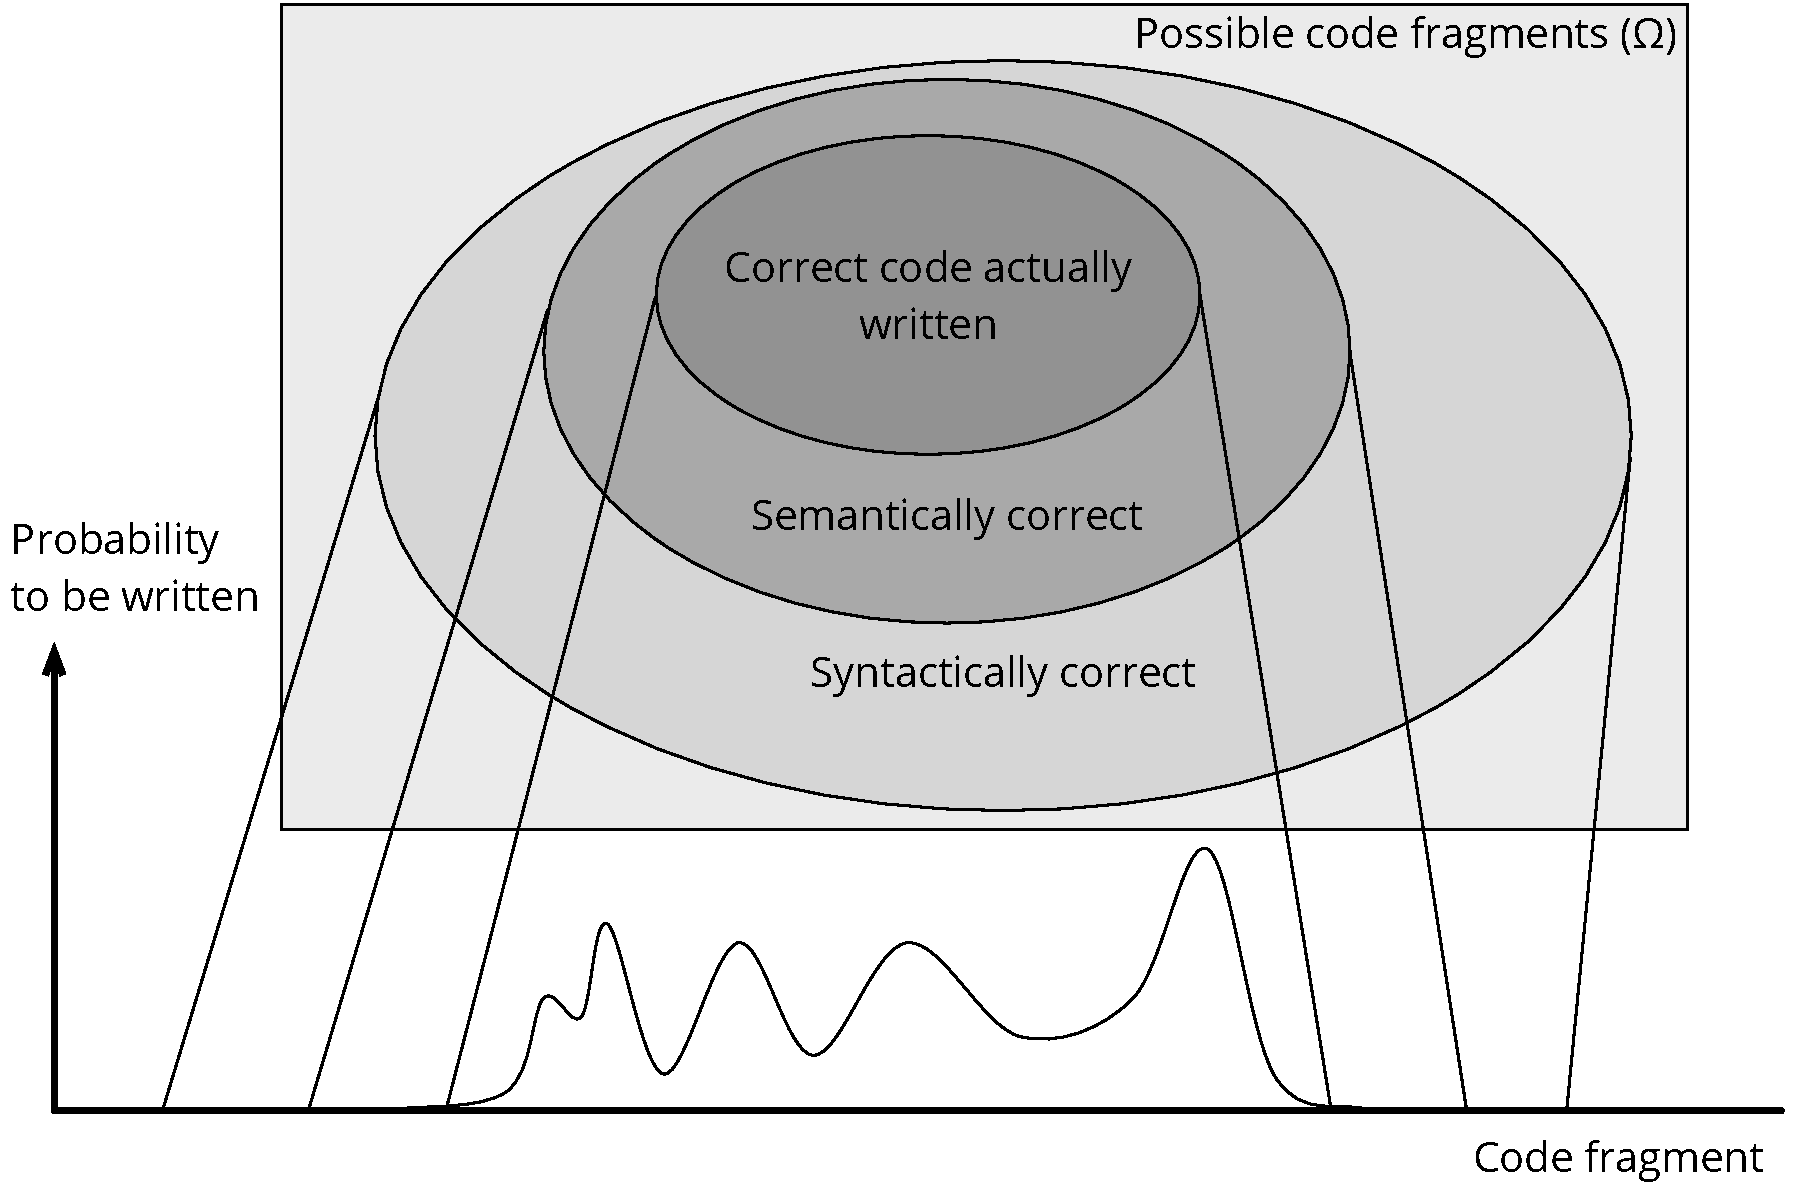
\includegraphics[width=0.9\textwidth]{figures/code_space_venn.pdf}
	\caption{An illustration of probabilities in code space}
	\label{fig:pdf_programs}
\end{figure}

To formalize our argumentation, we take a statistical view of program code.
Consider a formal language that describes the set of all possible programs.
For a program of fixed bounded size, this is a finite set $\Omega$.
For example, the set of syntactically correct C source files smaller than $1$~TiB in size is certainly bounded by $|\Omega| \leq 2^{2^{40}}$.
% For example, a source file $\omega \in \Omega$  under $10$ tebibyte (TiB), syntactically correct ones are certainly bounded by $|\Omega| = 10 \cdot 2^{40}$, probably a much lower number.
Out of the syntactically-correct programs, only a fraction successfully compiles, and only an even smaller fraction executes something that makes sense semantically.
Ideally, code written by developers falls into the subset of executable programs, as an even smaller subset.
However, in this subset of correctly written code, not every code fragment is going to be equally common.
A fragment like
\texttt{for(int i = 0; i < n; i++)} is probably going to be seen much more frequently than something like \texttt{(*(\&main+0x134))(x)}.
It is worth noting that there is a more nuanced discussion behind what constitutes a unit of code.
At this point, however, we can omit this discussion and consider the whole program as a unit, for simplicity of the argumentation.
%\se{Do we lose generality of our argument because of this? If not then we should say so.} % AG: I don't think we do, no.
Thus, there is an implicit \ac{pdf} $p$ on the discrete set of possible code units $\Omega$ which models the way programmers write code.\index{code distribution}
This is depicted in Figure~\ref{fig:pdf_programs}.
In reality, this is a highly dimensional space, and many challenges would arise in defining a proper geometry in such a space.
We depict the code space $\Omega$ as one-dimensional for illustrative purposes, just like the continuity of the \ac{pdf}, which we have no reason to assume.

\subsection{Representative Benchmarks}
\label{sec:representative_benchmarks}

In this statistical view of code, we can consider some precise questions: What does it mean for a collection of programs to be a benchmark?
More precisely, what does it mean for it to be representative, or what properties would be desirable of such a collection of programs?
Consider the examples depicted in Figure~\ref{fig:benchmark_types}.
This figure depicts histograms for three kinds of collections of programs along the (implicit) \ac{pdf} described in Figure~\ref{fig:pdf_programs}.
We think of an idealized abscissa dimension, with a proper metric, such that programs that are semantically close are close on this dimension.
Obviously, a multi-dimensional formalization would be better for this, but we stick to a single dimension for the intuition provided by the figures.
Thus, a bin in the histogram might contain a single program but represent a large category of mostly very closely related programs.

\begin{figure}[h]
	\centering
	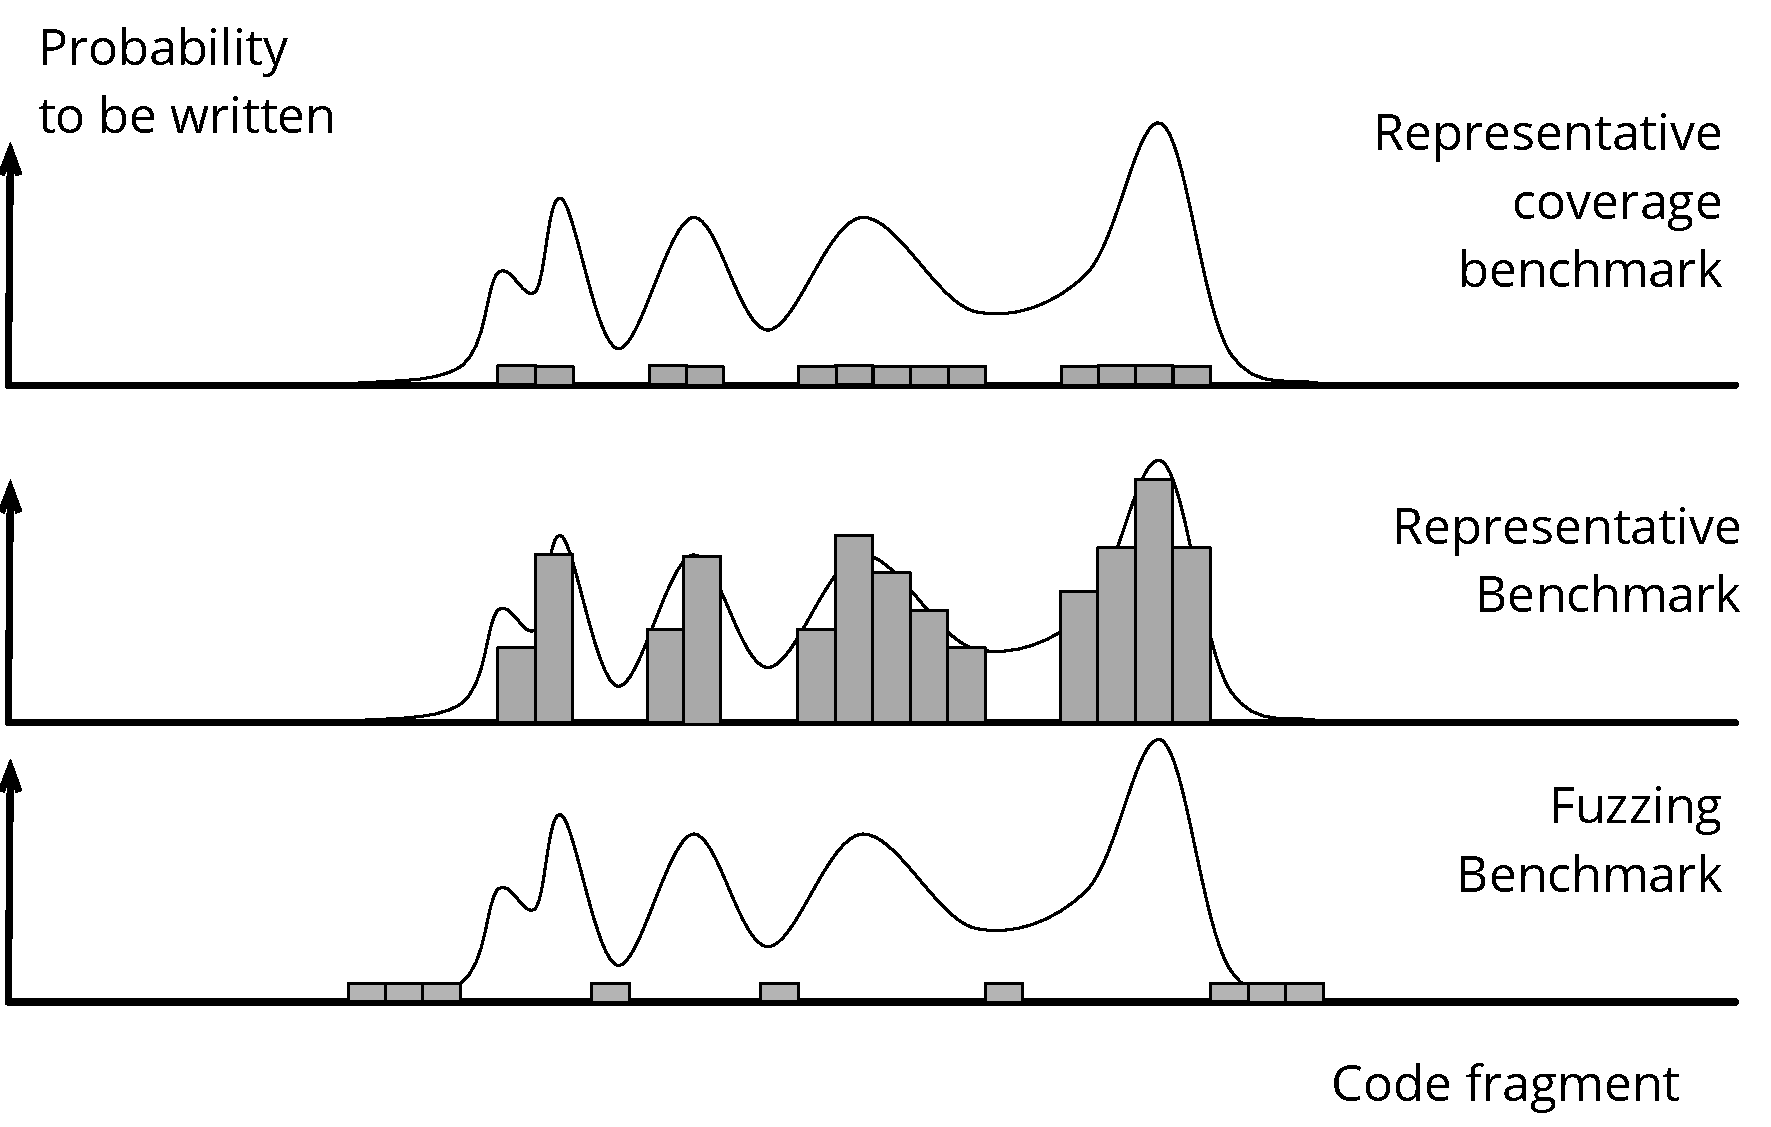
\includegraphics[width=0.9\textwidth]{figures/benchmark_types.pdf}
	\caption{An illustration of different types of benchmarks}
	\label{fig:benchmark_types}
\end{figure}

The first kind of collection depicted, labeled as a ``representative coverage benchmark'', has a handful of programs, each of which correspond to a different category in the space of probable programs.\index{representative coverage benchmark}
Programs that could be written by a human, but where it is unlikely that this will happen, are not covered by this type of benchmark. Furthermore, for every type or category of code fragments, there is only one representative example in the set.
In particular, programs that are moderately likely will be represented just as much as programs that are extremely likely to be written. This, in a sense, overrepresents the former and underrepresents the latter.

The second kind depicted, labeled as ``representative benchmark'', removes this imbalance. It is similar to the ``representative coverage benchmark'', but the difference is that in this kind of collection, programs appear with a relative frequency that is roughly in line with their probability to be written.
A benchmark of this kind would probably have more programs than a ``representative coverage benchmark'', without including significantly more types of programs or behaviors.

Finally, a ``fuzzing benchmark'' is a collection that does the opposite of a ``representative coverage benchmark''. It has programs covering those programs that are unlikely to be written by a human, but possible: The corner cases.\index{fuzzing benchmark}

%This pdf is what a generative model can learn.
%More formally, consider the generative model of code learning from these samples.
%Generative models are a class of machine learning problems that learn an unknown probability distribution for a random variable~\cite{vapnik}.
\subsection{Sample use cases}

We argue that what kind of benchmark is most appropriate depends on the use case. To illustrate this, we will explain two large classes of use-cases that require benchmarks. This certainly does not constitute an exhaustive classification, but will hopefully help clarify how the benchmark choice is nuanced.

\subsubsection{Testing}
\label{sec:testing}

A very common use case for benchmarking is testing. Assume we have developed a compiler optimization\footnote{A good mapping heuristic in software synthesis can be considered a compiler optimization in this context.} and want to see how good it works.
For this, we want to find out, in case someone writes a program and tries our optimization on it, how we can expect it to behave.
More formally, we have a property $\mathcal{P}$ of code, like the speedup obtained by applying our compiler optimization.
We want to calculate the expected value $E[\mathcal{P}]$ over the implicit \ac{pdf} of writing the code we use our compiler on\footnote{Technically, using the compiler is a conditional clause on the probability of a piece of code to be written by a human.}.

For testing, we argue that we want a \emph{representative} benchmark. Ideally, we would get a set of programs $x_1, \ldots, x_l \sim p$ \acs{i.i.d.}, where $p$ is the implicit \ac{pdf} of code been written\footnote{A compelling case can be made that in some cases it's the ``dynamic'' property of the probability that a piece of code will be \emph{executed}, not necessarily written, that is most interesting here.}.
The expected value $E[\mathcal{P}]$ can thus be approximated arbitrarily well with growing sample size $l$.
We do this because, in our example, we assume that the users of our compiler will also draw from this distribution $p$, and thus $E[\text{speedup}]$ tells us what speedup the users can expect to get out of our optimization.

If we use a ``representative coverage benchmark'', we can get a skewed result, because of the over- and underrepresentation of program types in this kind of benchmark.
Thus, if our optimization works extremely well for a small class of programs with a moderate chance of occurring, and not so well with the most common types of programs, our testing would return wrong results.
It would tell us that our optimization is likeley to improve our program, by overshooting the weight given to the moderately common class where it serves well.
In practice, however, our optimization would be unlikeley to bring much improvement in this case, if we expect our compiler to be used by everyone.

\subsubsection{Tuning a Heuristic}
\label{sec:tuning}

Another common use case is tuning a heuristic. Consider again a compiler optimization as an example. In this case, however, instead of having a finished optimization that we want to test, we are designing the optimization by tuning a heuristic that is part of it.
We want the heuristic to be tuned such that the optimization works best (which we would asses e.g. by testing, the other use-case).
Training machine learning models also falls under this category, and is thus likely that this use case will continue to increase in its importance in the feature.

For tuning the heuristic, an argument can be made for all three kinds of benchmarks from Figure~\ref{fig:benchmark_types}. It depends on the heuristic.
Assume we're dealing with a code transformation (e.g. converting Python 2 code automatically into Python 3),  which either it works or it doesn't. We want to optimize the parameters of our heuristic so that it works on the most cases possible.
In this case we probably want a ``fuzzing benchmark'', to be sure we cover the corner cases, or better yet, a combination of a ``fuzzing benchmark'' and a ``representative coverage benchmark''.
On the other hand, if the heuristic is something like a transformation expected to speed up the execution, then the argument for a ``representative benchmark'' is basically the same as for testing.
We want it maximize the expected value of this speedup.
An important distinction between heuristics pertains the way the parameters are set. Depending on how they are updated, repeatedly seeing similar code examples might be useless or even counter-productive, such that a ``representative coverage benchmark'' might be best suited.

More importantly yet is the process of designing the heuristic, before it is tuned. Usually this process is iterative. In it, having to look at the corner cases is common, too.
Arguments for all the discussed kinds of benchmarks can thus be made in similar fashion for the process of designing a heuristic, depending on specific goals.
For our methods improving software synthesis, we mostly want ``representative coverage benchmarks''.


\section{KPN Benchmarks}
\label{sec:kpn_benchmarks}
The \mocasin framework supports three input formats at the time of this writing: \texttt{tgff},\texttt{MAPS} and \texttt{sdf3}.
We will discuss the first two for benchmarking here, while the \texttt{sdf3} format will be discussed in Section~\ref{sec:level_graphs}.

\subsection{CPN Benchmarks}

The first input format for \mocasin is the \texttt{MAPS} format, which uses benchmarks written in the \ac{CPN} language (cf. Section~\ref{kpn_basic}).
A \ac{CPN} application is compiled using the \ac{MAPS} flow, which evolved into the commercial tool suite from SLX.
SLX generously provided access to their tool suite for this benchmarking, as well as some \ac{CPN} benchmarks. 

The tool flow compiles an application using a \acp{pthread} back-end with instrumentation to record all tokens read and written in a trace.
Since this traces are deterministic and depend only on the inputs, not on the execution order, they can be used to replay and simulate the execution (cf. Section~\ref{sec:simulating_mappings}).
In an instrumented run, the \ac{MAPS} flow also executes each process in isolation (with the stored tokens), gathering information about the precise instructions executed.
This is used for performance estimation using an abstract processor model\cite{eusse2014pre}.
The performance estimation for each process, together with the execution traces can then be used to simulate a mapping with \mocasin, as explain in Section~\ref{sec:simulating_mappings}.
This is summarized in Figure~\ref{fig:maps_flow}.

\begin{figure}[h]
	\centering
\resizebox{0.8\textwidth}{!}{
   \begin{tikzpicture}
     \begin{scope}[scale=1/2,every node/.append style={scale=1/2}]
%little cores
\node (pe1) at ({-1.5},{4}) [draw,minimum width=2.5cm,align=center,minimum height=2cm, fill=green!30] {\huge PE$_1$};
\node (L1-pe1) at (-1.5,2.5) [draw,minimum width=2.5cm,align=center,minimum height=1.5cm, fill=blue!30] {\huge L1\$};
\node (pe2) at (-1.5+3,4) [draw,minimum width=2.5cm,align=center,minimum height=2cm, fill=green!30] {\huge PE$_2$};
\node (L1-pe2) at (-1.5+3,2.5) [draw,minimum width=2.5cm,align=center,minimum height=1.5cm, fill=blue!30] {\huge L1\$};
\node (pe3) at (-1.5,4+4) [draw,minimum width=2.5cm,align=center,minimum height=2cm, fill=green!30] {\huge PE$_3$};
\node (L1-pe3) at (-1.5,2.5+4) [draw,minimum width=2.5cm,align=center,minimum height=1.5cm, fill=blue!30] {\huge L1\$};
\node (pe4) at (-1.5+3,4+4) [draw,minimum width=2.5cm,align=center,minimum height=2cm, fill=green!30] {\huge PE$_4$};
\node (L1-pe4) at (-1.5+3,2.5+4) [draw,minimum width=2.5cm,align=center,minimum height=1.5cm, fill=blue!30] {\huge L1\$};

%big cores
\node (pe1) at ({6.5-1.5},{4}) [draw,minimum width=2.5cm,align=center,minimum height=2cm, fill=green!60] {\huge PE$_5$};
\node (L1-pe1) at (6.5-1.5,2.5) [draw,minimum width=2.5cm,align=center,minimum height=1.5cm, fill=blue!30] {\huge L1\$};
\node (pe2) at (6.5-1.5+3,4) [draw,minimum width=2.5cm,align=center,minimum height=2cm, fill=green!60] {\huge PE$_6$};
\node (L1-pe2) at (6.5-1.5+3,2.5) [draw,minimum width=2.5cm,align=center,minimum height=1.5cm, fill=blue!30] {\huge L1\$};
\node (pe3) at (6.5-1.5,4+4) [draw,minimum width=2.5cm,align=center,minimum height=2cm, fill=green!60] {\huge PE$_7$};
\node (L1-pe3) at (6.5-1.5,2.5+4) [draw,minimum width=2.5cm,align=center,minimum height=1.5cm, fill=blue!30] {\huge L1\$};
\node (pe4) at (6.5-1.5+3,4+4) [draw,minimum width=2.5cm,align=center,minimum height=2cm, fill=green!60] {\huge PE$_8$};
\node (L1-pe4) at (6.5-1.5+3,2.5+4) [draw,minimum width=2.5cm,align=center,minimum height=1.5cm, fill=blue!30] {\huge L1\$};


\node (L2-little) at (0,0) [draw,minimum width=6cm,align=center,minimum height=1.5cm, fill=blue!55] {\huge L2\$};
\node (L2-big) at (6.5,0) [draw,minimum width=6cm,align=center,minimum height=1.5cm, fill=blue!55] {\huge L2\$};
\node (DRAM) at (3.25,-2.5) [minimum width=12.5cm,align=center,minimum height=2cm, fill=blue!85] {\huge DRAM};

%tasks
\node[ellipse,fill=yellow!60] (t1) at (-1.5+3,4) {\Huge t$_1$};
\node[ellipse,fill=yellow!60] (t2) at ({-1.5},{4}) {\Huge t$_2$};
\draw (0,0) edge[-{latex},out=00,in=270,looseness=1,line width=1.2mm, color=yellow!80] (t1);
\draw (0,0) edge[-{latex},out=180,in=270,looseness=1,line width=1.2mm, color=yellow!80] (t2);
\end{scope}

\begin{scope}[xshift = 250,yshift=80]
\node[ellipse,fill=yellow!60] (t1-m) {\Huge t$_1$};
\node[ellipse,fill=yellow!60, below = of t1-m] (t2-m) {\Huge t$_2$};
\draw[{latex}-{latex},line width=1mm, color=yellow!80] (t1-m) -- (t2-m) node [right] (l1) {};

\node[ellipse,fill=green!30, right = 3cm of t1-m] (pe1) {PE$_1$};
\node[ellipse,fill=green!30, right = 3cm of t2-m] (pe2) {PE$_2$};
\draw[latex-latex,color=blue!55] (pe1.south) -- (pe2.north) node [left] (l2) {};
\draw[|->] (1,-1.1) -- node [above] {$m$} (3.3,-1.1);
\end{scope}
   \end{tikzpicture}
 }
   \caption{Benchmarks in the \ac{MAPS} flow. TODO: fix figure}
   \label{fig:maps_flow}
\end{figure}


We use three \ac{CPN} benchmarks for evaluation.
The first benchmark is the audio filter example as seen in Chapter~\ref{chap:mapping}, which takes a stereo file and implements a band-pass filter after transforming to the frequency, and transforming it back afterwards.
This benchmark has $8$ processes and $15$ channels (some channels for parameters are not depicted in Figure~\ref{fig:audio_filter_graph}).
The second benchmark we consider is an embedded pedestrian-recognition application using an algorithm based on the \ac{HOG} technique\index{HOG}.
This benchmark was kindly provided by SLX and consists of $10$ processes with $33$ channels.
Finally, we use a speaker recognition application, as described in~\cite{bouraoui2019comparing}.
Figure~\ref{fig:speaker_recognition} shows the graph of the speaker recognition application. \index{speaker recognition}
The speaker recognition application has $12$ processes and $33$ channels.

\begin{figure}[h]
	\centering
\resizebox{0.9\textwidth}{!}{
     
\begin{tikzpicture}[>=latex,line join=bevel,]
\Large%
\node (process_source) at (715.0bp,542.0bp) [draw,ellipse] {source};
  \node (process_readwave_stage1) at (438.0bp,469.0bp) [draw,ellipse] {readwave\_stage1};
  \node (process_ShifterDLP) at (759.0bp,159.0bp) [draw,ellipse] {ShifterDLP};
  \node (process_Worker_0) at (340.0bp,84.0bp) [draw,ellipse] {Worker\_0};
  \node (process_Worker_1) at (189.0bp,84.0bp) [draw,ellipse] {Worker\_1};
  \node (process_Worker_2) at (813.0bp,84.0bp) [draw,ellipse] {Worker\_2};
  \node (process_Worker_3) at (512.0bp,84.0bp) [draw,ellipse] {Worker\_3};
  \node (process_hamming_stage2) at (446.0bp,393.0bp) [draw,ellipse] {hamming\_stage2};
  \node (process_FFT_stage3) at (394.0bp,315.0bp) [draw,ellipse] {FFT\_stage3};
  \node (process_melFreqWrap_stage4) at (461.0bp,237.0bp) [draw,ellipse] {melFreqWrap\_stage4};
  \node (process_DCT_stage5) at (378.0bp,159.0bp) [draw,ellipse] {DCT\_stage5};
  \node (process_sink) at (468.0bp,10.0bp) [draw,ellipse] {sink};
  \draw [->] (process_source) ..controls (651.96bp,525.39bp) and (542.33bp,496.49bp)  .. (process_readwave_stage1);
  \definecolor{strokecol}{rgb}{0.0,0.0,0.0};
  \pgfsetstrokecolor{strokecol}
  \draw (631.0bp,507.0bp) node {testFile};
  \draw [->] (process_source) ..controls (709.4bp,506.66bp) and (697.53bp,415.81bp)  .. (715.0bp,344.0bp) .. controls (721.86bp,315.8bp) and (736.6bp,313.78bp)  .. (745.0bp,286.0bp) .. controls (756.02bp,249.54bp) and (758.56bp,204.86bp)  .. (process_ShifterDLP);
  \draw (745.5bp,354.0bp) node {speakers};
  \draw [->] (process_source) ..controls (755.59bp,526.33bp) and (798.0bp,504.12bp)  .. (798.0bp,469.0bp) .. controls (798.0bp,469.0bp) and (798.0bp,469.0bp)  .. (798.0bp,237.0bp) .. controls (798.0bp,214.47bp) and (784.82bp,191.78bp)  .. (process_ShifterDLP);
  \draw (828.0bp,354.0bp) node {nbSpeakers};
  \draw [->] (process_source) ..controls (576.29bp,540.18bp) and (96.0bp,530.0bp)  .. (96.0bp,469.0bp) .. controls (96.0bp,469.0bp) and (96.0bp,469.0bp)  .. (96.0bp,198.0bp) .. controls (96.0bp,128.72bp) and (162.54bp,139.78bp)  .. (226.0bp,112.0bp) .. controls (249.48bp,101.72bp) and (277.39bp,94.787bp)  .. (process_Worker_0);
  \draw (126.0bp,315.0bp) node {nbSpeakers};
  \draw [->] (process_source) ..controls (596.11bp,540.67bp) and (252.22bp,535.46bp)  .. (145.0bp,516.0bp) .. controls (78.343bp,503.9bp) and (0.0bp,536.75bp)  .. (0.0bp,469.0bp) .. controls (0.0bp,469.0bp) and (0.0bp,469.0bp)  .. (0.0bp,159.0bp) .. controls (0.0bp,126.93bp) and (95.203bp,102.6bp)  .. (process_Worker_1);
  \draw (30.0bp,315.0bp) node {nbSpeakers};
  \draw [->] (process_source) ..controls (779.29bp,536.55bp) and (861.08bp,528.13bp)  .. (887.0bp,516.0bp) .. controls (915.51bp,502.65bp) and (940.0bp,500.48bp)  .. (940.0bp,469.0bp) .. controls (940.0bp,469.0bp) and (940.0bp,469.0bp)  .. (940.0bp,159.0bp) .. controls (940.0bp,118.16bp) and (890.7bp,99.094bp)  .. (process_Worker_2);
  \draw (970.0bp,315.0bp) node {nbSpeakers};
  \draw [->] (process_source) ..controls (753.48bp,535.5bp) and (775.6bp,528.89bp)  .. (791.0bp,516.0bp) .. controls (805.04bp,504.26bp) and (803.04bp,496.48bp)  .. (811.0bp,480.0bp) .. controls (835.25bp,429.75bp) and (848.12bp,418.72bp)  .. (859.0bp,364.0bp) .. controls (866.73bp,325.09bp) and (844.0bp,315.68bp)  .. (844.0bp,276.0bp) .. controls (844.0bp,276.0bp) and (844.0bp,276.0bp)  .. (844.0bp,159.0bp) .. controls (844.0bp,128.18bp) and (821.12bp,124.62bp)  .. (793.0bp,112.0bp) .. controls (751.73bp,93.475bp) and (623.96bp,87.108bp)  .. (process_Worker_3);
  \draw (886.0bp,315.0bp) node {nbSpeakers};
  \draw [->] (process_readwave_stage1) ..controls (437.35bp,448.19bp) and (437.42bp,434.14bp)  .. (439.0bp,422.0bp) .. controls (439.34bp,419.39bp) and (439.82bp,416.68bp)  .. (process_hamming_stage2);
  \draw (477.0bp,431.0bp) node {tokenFrame};
  \draw [->] (process_readwave_stage1) ..controls (379.01bp,452.8bp) and (353.4bp,439.97bp)  .. (366.0bp,422.0bp) .. controls (370.53bp,415.54bp) and (385.21bp,409.42bp)  .. (process_hamming_stage2);
  \draw (399.5bp,431.0bp) node {nbFrames};
  \draw [->] (process_readwave_stage1) ..controls (368.61bp,452.94bp) and (330.07bp,436.28bp)  .. (315.0bp,404.0bp) .. controls (300.78bp,373.56bp) and (336.51bp,345.88bp)  .. (process_FFT_stage3);
  \draw (348.5bp,393.0bp) node {nbFrames};
  \draw [->] (process_readwave_stage1) ..controls (490.25bp,454.88bp) and (509.76bp,447.58bp)  .. (515.0bp,440.0bp) .. controls (521.8bp,430.17bp) and (517.58bp,392.58bp)  .. (510.0bp,382.0bp) .. controls (499.36bp,367.13bp) and (483.42bp,379.03bp)  .. (473.0bp,364.0bp) .. controls (461.49bp,347.39bp) and (460.29bp,289.93bp)  .. (process_melFreqWrap_stage4);
  \draw (504.0bp,354.0bp) node {sampleRate};
  \draw [->] (process_readwave_stage1) ..controls (499.29bp,456.02bp) and (523.23bp,448.63bp)  .. (530.0bp,440.0bp) .. controls (556.38bp,406.39bp) and (547.73bp,384.78bp)  .. (535.0bp,344.0bp) .. controls (524.06bp,308.94bp) and (497.16bp,275.25bp)  .. (process_melFreqWrap_stage4);
  \draw (573.5bp,354.0bp) node {nbFrames};
  \draw [->] (process_readwave_stage1) ..controls (366.91bp,456.97bp) and (333.95bp,449.22bp)  .. (323.0bp,440.0bp) .. controls (311.24bp,430.1bp) and (283.03bp,358.49bp)  .. (277.0bp,326.0bp) .. controls (275.21bp,316.39bp) and (273.67bp,313.19bp)  .. (277.0bp,304.0bp) .. controls (280.55bp,294.21bp) and (285.74bp,294.32bp)  .. (292.0bp,286.0bp) .. controls (319.68bp,249.21bp) and (349.2bp,204.18bp)  .. (process_DCT_stage5);
  \draw (310.5bp,315.0bp) node {nbFrames};
  \draw [->] (process_readwave_stage1) ..controls (359.95bp,457.88bp) and (320.41bp,449.98bp)  .. (307.0bp,440.0bp) .. controls (244.11bp,393.2bp) and (240.75bp,361.87bp)  .. (221.0bp,286.0bp) .. controls (201.08bp,209.46bp) and (279.95bp,132.74bp)  .. (process_Worker_0);
  \draw (254.5bp,276.0bp) node {nbFrames};
  \draw [->] (process_readwave_stage1) ..controls (350.98bp,458.46bp) and (299.37bp,450.17bp)  .. (281.0bp,440.0bp) .. controls (276.67bp,437.6bp) and (150.68bp,295.97bp)  .. (147.0bp,286.0bp) .. controls (123.05bp,221.2bp) and (159.03bp,139.38bp)  .. (process_Worker_1);
  \draw (180.5bp,276.0bp) node {nbFrames};
  \draw [->] (process_readwave_stage1) ..controls (516.16bp,456.87bp) and (559.24bp,448.55bp)  .. (575.0bp,440.0bp) .. controls (594.89bp,429.21bp) and (598.65bp,422.96bp)  .. (611.0bp,404.0bp) .. controls (619.32bp,391.22bp) and (698.41bp,157.91bp)  .. (710.0bp,148.0bp) .. controls (738.68bp,123.46bp) and (763.82bp,153.94bp)  .. (793.0bp,130.0bp) .. controls (801.02bp,123.42bp) and (805.91bp,113.0bp)  .. (process_Worker_2);
  \draw (695.5bp,276.0bp) node {nbFrames};
  \draw [->] (process_readwave_stage1) ..controls (506.22bp,459.24bp) and (530.06bp,452.16bp)  .. (549.0bp,440.0bp) .. controls (585.68bp,416.44bp) and (596.37bp,405.07bp)  .. (611.0bp,364.0bp) .. controls (622.69bp,331.17bp) and (602.29bp,347.91bp)  .. (526.0bp,130.0bp) .. controls (523.05bp,121.56bp) and (520.11bp,112.14bp)  .. (process_Worker_3);
  \draw (619.5bp,276.0bp) node {nbFrames};
  \draw [->] (process_hamming_stage2) ..controls (387.39bp,379.74bp) and (365.05bp,372.4bp)  .. (359.0bp,364.0bp) .. controls (353.8bp,356.79bp) and (355.22bp,352.04bp)  .. (359.0bp,344.0bp) .. controls (361.15bp,339.42bp) and (364.42bp,335.32bp)  .. (process_FFT_stage3);
  \draw (404.5bp,354.0bp) node {token\_H\_Frame};
  \draw [->] (process_FFT_stage3) ..controls (368.92bp,294.27bp) and (355.69bp,278.54bp)  .. (365.0bp,266.0bp) .. controls (370.45bp,258.65bp) and (387.61bp,252.45bp)  .. (process_melFreqWrap_stage4);
  \draw (411.5bp,276.0bp) node {spectrumVector};
  \draw [->] (process_melFreqWrap_stage4) ..controls (455.42bp,215.14bp) and (449.43bp,198.66bp)  .. (439.0bp,188.0bp) .. controls (432.32bp,181.17bp) and (423.7bp,175.75bp)  .. (process_DCT_stage5);
  \draw (476.0bp,198.0bp) node {logms};
  \draw [->] (process_melFreqWrap_stage4) ..controls (401.05bp,222.99bp) and (380.7bp,215.94bp)  .. (375.0bp,208.0bp) .. controls (369.29bp,200.05bp) and (369.31bp,189.38bp)  .. (process_DCT_stage5);
  \draw (405.0bp,198.0bp) node {codesize};
  \draw [->] (process_DCT_stage5) ..controls (352.15bp,144.28bp) and (344.94bp,137.88bp)  .. (341.0bp,130.0bp) .. controls (337.07bp,122.15bp) and (336.33bp,112.57bp)  .. (process_Worker_0);
  \draw (374.5bp,121.0bp) node {dct\_frame};
  \draw [->] (process_DCT_stage5) ..controls (320.25bp,148.08bp) and (290.21bp,140.59bp)  .. (265.0bp,130.0bp) .. controls (245.45bp,121.79bp) and (224.98bp,109.13bp)  .. (process_Worker_1);
  \draw (298.5bp,121.0bp) node {dct\_frame};
  \draw [->] (process_DCT_stage5) ..controls (437.21bp,147.43bp) and (472.09bp,139.55bp)  .. (502.0bp,130.0bp) .. controls (522.13bp,123.57bp) and (525.51bp,117.15bp)  .. (546.0bp,112.0bp) .. controls (587.21bp,101.63bp) and (705.18bp,91.829bp)  .. (process_Worker_2);
  \draw (579.5bp,121.0bp) node {dct\_frame};
  \draw [->] (process_DCT_stage5) ..controls (402.04bp,135.83bp) and (422.08bp,117.21bp)  .. (431.0bp,112.0bp) .. controls (444.88bp,103.88bp) and (461.47bp,97.63bp)  .. (process_Worker_3);
  \draw (464.5bp,121.0bp) node {dct\_frame};
  \draw [->] (process_ShifterDLP) ..controls (722.89bp,145.81bp) and (706.95bp,138.65bp)  .. (694.0bp,130.0bp) .. controls (684.33bp,123.54bp) and (685.62bp,116.75bp)  .. (675.0bp,112.0bp) .. controls (671.7bp,110.52bp) and (472.31bp,94.518bp)  .. (process_Worker_0);
  \draw (713.5bp,121.0bp) node {SPW0};
  \draw [->] (process_ShifterDLP) ..controls (694.78bp,152.11bp) and (659.72bp,144.83bp)  .. (632.0bp,130.0bp) .. controls (621.74bp,124.51bp) and (623.68bp,116.61bp)  .. (613.0bp,112.0bp) .. controls (548.63bp,84.198bp) and (367.92bp,99.204bp)  .. (298.0bp,94.0bp) .. controls (275.89bp,92.355bp) and (251.3bp,90.132bp)  .. (process_Worker_1);
  \draw (651.5bp,121.0bp) node {SPW1};
  \draw [->] (process_ShifterDLP) ..controls (805.07bp,149.04bp) and (819.08bp,141.99bp)  .. (827.0bp,130.0bp) .. controls (832.41bp,121.82bp) and (829.9bp,111.45bp)  .. (process_Worker_2);
  \draw (849.5bp,121.0bp) node {SPW2};
  \draw [->] (process_ShifterDLP) ..controls (754.76bp,137.94bp) and (749.1bp,120.79bp)  .. (737.0bp,112.0bp) .. controls (722.59bp,101.53bp) and (616.05bp,91.865bp)  .. (process_Worker_3);
  \draw (769.5bp,121.0bp) node {SPW3};
  \draw [->] (process_Worker_0) ..controls (369.18bp,65.42bp) and (393.5bp,50.255bp)  .. (415.0bp,38.0bp) .. controls (425.04bp,32.279bp) and (436.33bp,26.256bp)  .. (process_sink);
  \draw (447.5bp,47.0bp) node {str\_min\_0};
  \draw [->] (process_Worker_1) ..controls (233.12bp,65.694bp) and (277.07bp,48.558bp)  .. (316.0bp,38.0bp) .. controls (359.09bp,26.314bp) and (410.37bp,17.991bp)  .. (process_sink);
  \draw (348.5bp,47.0bp) node {str\_min\_1};
  \draw [->] (process_Worker_2) ..controls (720.86bp,64.236bp) and (558.73bp,29.461bp)  .. (process_sink);
  \draw (713.5bp,47.0bp) node {str\_min\_2};
  \draw [->] (process_Worker_3) ..controls (499.14bp,62.37bp) and (487.54bp,42.861bp)  .. (process_sink);
  \draw (527.5bp,47.0bp) node {str\_min\_3};
%
\end{tikzpicture}

 }
   \caption{The \ac{KPN} graph of the speaker recognition application.}
   \label{fig:speaker_recognition}
\end{figure}

\subsection{The E3S Benchmarks}

The second input of \mocasin we use for benchmarking is \texttt{tgff}.
The \texttt{tgff} format comes from \acf{tgff}, a random task graph generator~\cite{dick1998tgff}. 
However, the same author also published a benchmark suite, the \ac{E3S}~\cite{e3s}.
Based on data from the Embedded Microprocessor Benchmark Consortium, the suite provides task graphs and processor execution times for applications from multiple embedded domains.
In total, the \ac{E3S} boasts Table~\ref{tab:e3s} summarizes the applications.

\begin{table*}[t]
  %\footnotesize
  \caption{Summary of applications in the \ac{E3S}}
  \begin{center}
    \begin{tabular}{lll}
      %\hline
      Domain & No. of task graphs & tasks per graph\\
      \hline
      auto-indust & 4 & 4-9\\
      networking & 4 & 1-4\\
      telecom & 9 & 2-6\\
      consumer & 2 & 5-7\\
      office-automation & 1 & 5\\
    \end{tabular}
    \label{tab:e3s}
  \end{center}
  \vspace{-0.5cm}
\end{table*}

The processors and architectures in the \ac{E3S} are generally not \acp{MPSoC}, most of them are single-core systems.
This comes mostly because the benchmark suite is pretty dated, being over $20$ years old at the time of this writing.
Unfortunately, benchmarks are generally scarce.
The methods investigated in this thesis here have more to do with the trends than the actual numbers, which is why using such a dated benchmark is still adequate.
We expect the relative performance of mapping algorithms on the \ac{E3S} benchmarks to be similar to that on present and future applications.

A significant focus of the methods we will evaluate with these benchmarks is on the multicore architectures.
To overcome the limitation of the single-core nature of the \ac{E3S}, we use the same method as in~\cite{schwarzer2017symmetry}.
We use the architecture topology of a modern multicore, including the frequencies, as well as the memory subsystem with its latency and bandwidth, and scale the numbers from the \ac{E3S} for each of the cores of the modern multicore.
This gives a realistic scenario, albeit not simulating a concrete instance of the architecture.
In~\cite{schwarzer2017symmetry} the authors do this to create architectures with a regular mesh structure, with less realistic topologies like heterogeneous meshes with randomly placed cores.
Instead, we use the topologies from actual existing systems like the HAEC~\cite{HAEC} or the Kalray MPPA3 Coolidge~\cite{coolidge} and map the processors in these architectures to those in the benchmark suite.
\section{Random Benchmarks and Level Graphs}
\label{sec:level_graphs}
The third category of inputs for \mocasin is \texttt{sdf3}, which uses the \ac{\SDFFF} framework~\cite{sdf3}.
This framework is based on \ac{TGFF}, adapted to the \ac{SDF} model of computation.
We will discuss \ac{SDF} more in detail in Chapter~\ref{chap:mocs}.
However, for the purposes of benchmarking as discussed here, both \ac{SDF} and task graphs can be considered as special cases of \ac{KPN}.
The random graph generation of the \ac{\SDFFF} framework allows multiple configurations on the types of graphs it generates, controlling the number of actors (processes) as well as the degree of connectivity in the graph, firing rates and execution times of the actors, or if the graph is acycilic.

Random benchmark generation has two main advantages over using fixed benchmarks. The first advantage is the amount of benchmarks, which is virtually unlimited with a random generation approach.
The second advantage is the control over the properties of the benchmarks.
Using \ac{\SDFFF} we can consider precisely what effect the properties of the graph have on the algorithms (e.g. its size, or connectivity), by generating benchmarks which have the desired parameters for the independent variable we are investigating.
The main disadvantage is obvious: random benchmarks are not as realistic as actual benchmarks.
It is not clear if we will find a graph like the one generated by \ac{\SDFFF} in a real-life application.

Since we have both the \ac{CPN} and the \ac{E3S} benchmarks, we will focus our evaluation on those.
Instead of discussing the graph generation in \ac{\SDFFF}, we will discuss random benchmark generation from a different type of graph, \emph{level graphs}\cite{goens_multiprog18}.
The main difference is that for the use-case for level graphs in~\cite{goens_multiprog18} we \textbf{do not} have better, realistic benchmarks we can use instead.

The context for benchmark generation we will discuss here are micro-service-oriented architectures.
Large internet companies like Facebook or Twitter have an infrastructure that consists of multiple micro-services that depend on each other~\cite{marlow2014haxl}.
A crucial factor for optimal performance is the amount of \ac{I/O} calls these micro-services make.
We will discuss the use case more in-depth in Chapter~\ref{chap:pl}. 
In this section we will only focus on the benchmark generation.

The micro-service-based infrastructures from large companies like Facebook or Twitter are the \acf{IP} of these companies and not in the public domain.
If, for example, we want to improve and compare a method for optimizing \ac{I/O} in Facebook's spam-fighting service~\cite{marlow2014haxl}, we cannot use a large representative benchmark sample from Facebook to test against their method.
Instead, we observe the general structure of the programs in their work and device a methodology for generating random benchmarks, with a method we call level graphs~\cite{goens_multiprog18}.

\begin{figure*}[th]
	\centering
	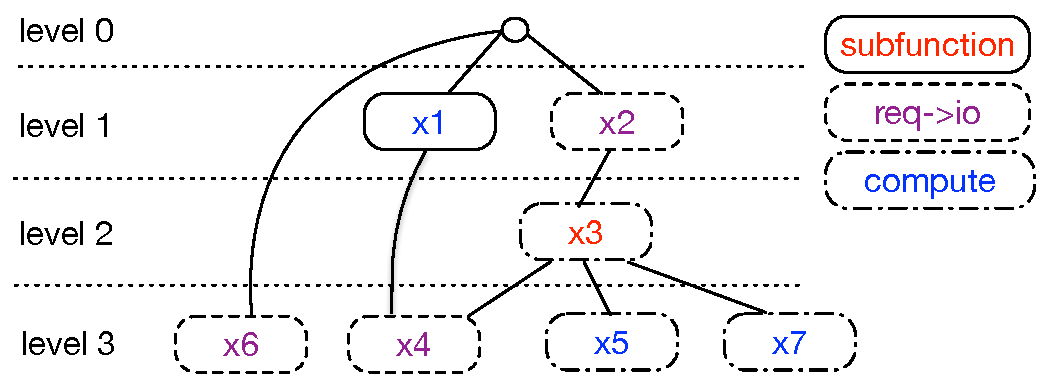
\includegraphics[width=\textwidth]{figures/level-graph.pdf}
	\caption{An example of a Level Graph. Reproduced from Figure~1 of \cite{goens_multiprog18}.}
	\label{fig:level_graph}
\end{figure*}

Figure~\ref{fig:level_graph} shows an example of a level graph. The graph depicted is a tree which is organized by levels, which are indexed with integer numbers.
The nodes in the graph are labeled as different kinds of node, namely \texttt{req$\rightarrow$io},\texttt{subfunction} and \texttt{compute}.
The graph depicted is designed to benchmark \ac{I/O} optimization, which is why the node labels are designed accordingly, reflecting \ac{I/O} calls and other computation,
as well as an additional \texttt{subfunction} node that creates nested benchmarks with additional function calls.
This is also by design, to test the use-case.

The idea behind level graphs is to reflect the intuition of \emph{locality} in code\index{locality in code}.
This intuition is based on the observation that long-rage dependencies in code are less common than short-ranged ones.
While programmers do sometimes refer back to identifiers defined far behind, it is far more common to define values before using them.
We interpret this as a statistical feature of the distribution of code as commonly written by humans (cf. Section~\ref{sec:representative_benchmarks}).
Levels in level graphs are thus designed to define the probability distribution of dependencies in graphs.

There are generally two accepted and common models of random graphs, the Erd\H{o}s-R\'{e}yni approach~\cite{erdosreyni} and the Gilbert approach~\cite{gilbert1959random}.
The former defines a uniform distribution over all graphs for a given number of nodes, while the latter defines the probabilities of the edges independently.
Our definition of \emph{Level Graphs}\index{level graph} is based on the Gilbert approach, but instead of having uniform probabilities, the probabilities are defined through the levels.
Concretely, a level graph $L = ((V,E),l)$ is a directed graph $(V,E)$ with a level function $l : V \rightarrow \mathbb{N}$ to the natural numbers, with the property that for all nodes $v,w \in V$ there can only be an edge $(v,w) \in E$ if the level of $v$ is smaller than that of $w$, i.e. $(v,w) \in E \Rightarrow l(v) < l(w)$.
To generate a probability distribution in level graphs we define the probability of the edge $(v,w) \in E$ to be as follows:
\[  p( (v,w) ) = \left\{
    \begin{array}{ll}
      0, & \text{ if } l(v) \geq l(w), \\
      2^{l(v)-l(w)}, & \text{ otherwise.}
    \end{array} \right. \]
The method can be generalized by choosing a different probability for the case where $l(v) < l(w)$.
The chosen value $2^{l(v)-l(w)}$ is, to an extent, arbitrary.
This probability definition ensures that dependencies are more common locally, between levels that are close by, discouraging but not prohibiting long-range dependencies.

A level graph can be used to generate code in different languages or back-ends, expressing the same computation.
In~\cite{goens_multiprog18} we implemented three back-ends for \ac{I/O} optimizing frameworks, one for Ohua/\"{Y}auhau~\cite{ertel_cc18} (see Section~\ref{sec:yauhau}), one for Twitter's Muse~\cite{muse} and one for Facebook's Haxl~\cite{marlow2014haxl}.
These back-ends are also based on different languages, namely Clojure and Haskell.
The abstract nature of level graphs allows us to generate code in different languages. %multiprog
\section{Machine Learning}
\label{sec:machine_learning}
In the previous two sections we have discussed multiple benchmarks in two different classes: hand-written benchmarks and randomly generated benchmarks.
We have discussed the advantages and disadvantages of both.
Hand-written benchmarks cost many person-hours to write and maintain, and are usually very limited due to \ac{IP}.
Random benchmarks can overcome the scarcity of hand written ones at the cost of accuracy, they are less realistic and not as useful for assessing how well a method will perform on real use-cases.
There is a third approach that sits in-between the two above, to use machine learning to generate benchmarks with realistic properties.
This section discusses this approach and its limitations.

\subsection{Generative models}
\label{sec:generative}

\begin{figure*}[th]
	\centering
	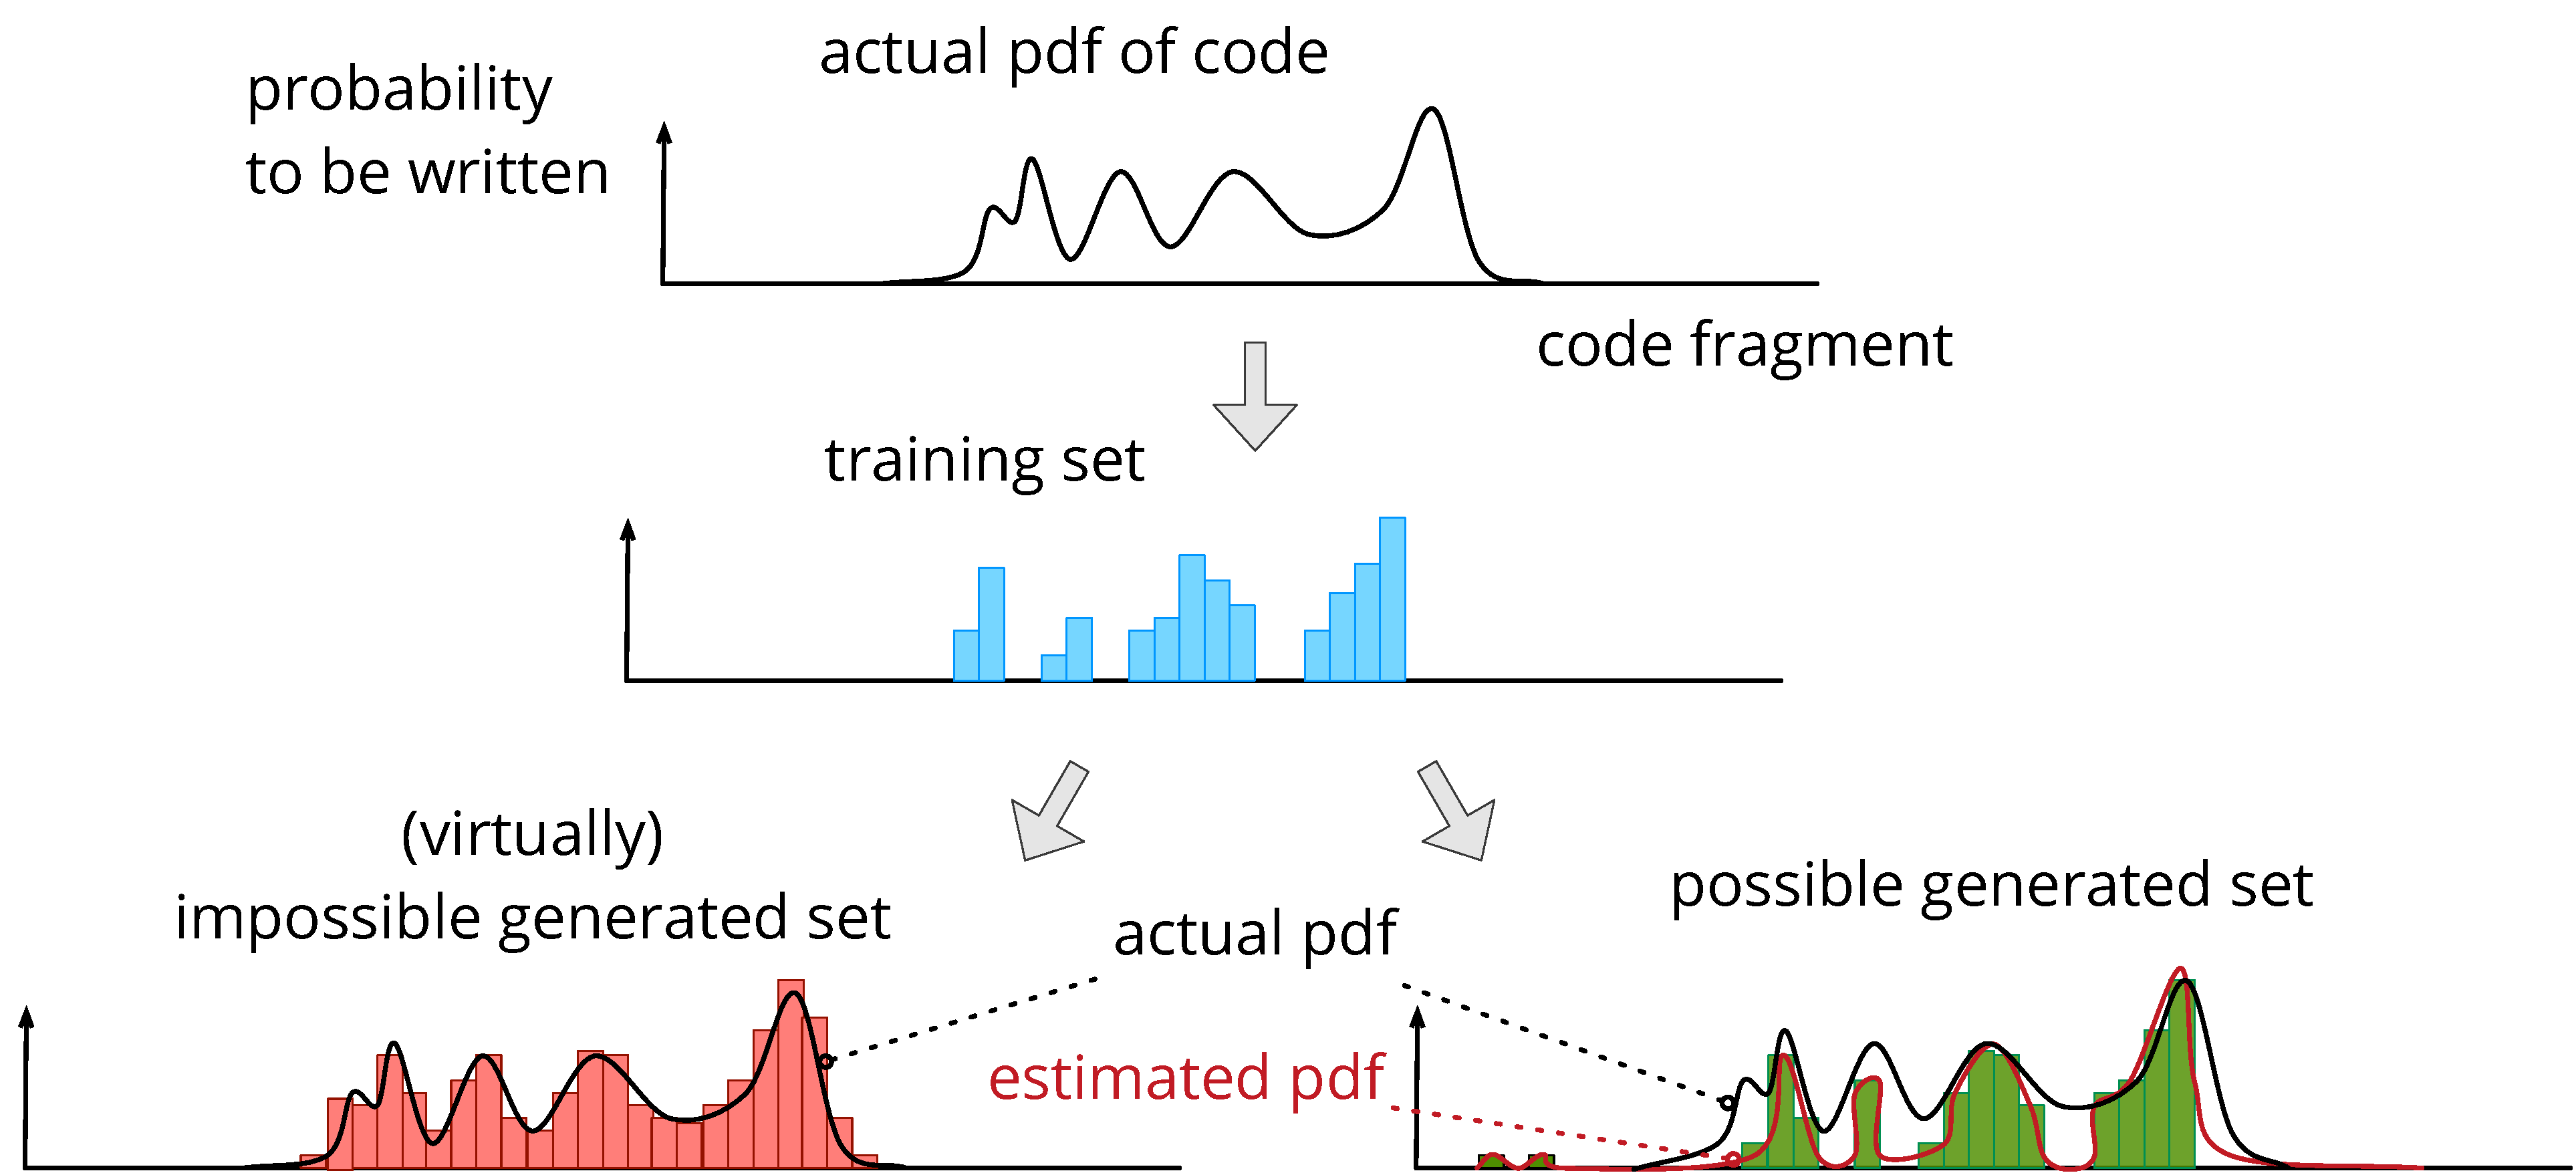
\includegraphics[width=\textwidth]{figures/illustration_histograms_ideal.pdf}
	\caption{An illustration of generative models in the Fischer-Wald setting.}
	\label{fig:histograms}
\end{figure*}

Machine learning models that could generate benchmarks fall under the general term ``generative models''.
There are different classes of generative models, however:
%Let again $p$ be the probability density function describing the probability of a programmer writing a piece of code $\omega \in \Omega$.
\begin{enumerate}
\item \label{fischer-wald} A model in the \textbf{Fischer-Wald setting} is a machine learning model solving the problem of density estimation~\cite{vapnik}. This means finding a probability $p'(t,\alpha_0)$ in a set of probabilities $\{ p'(t,\alpha) \mid \alpha \in \Lambda \}$ parametrized by elements of the parameter set $\Lambda$,
  such that for the risk functional $R(\alpha) = \int -\log(p'(t,\alpha)) dp(t)$, the value of $R(\alpha_0)$ is minimal over all $\alpha \in \Lambda$.
\item \label{conditional-estimation} A \textbf{conditional estimation} model can again mean a solution to a few different problems in different settings. For a random variable $Y$ over code, it estimates either the joint distribution $X \times Y$ or one of the conditional probabilities $p(y \mid X = x)$ or $p(x \mid Y = y)$, where $X$ is the random variable representing a piece of code (i.e. $X(\omega) = \omega$, the identity on $\Omega$)~\cite{vapnik}.

\end{enumerate}

Conditional estimation generative models have plenty of applications.
For example, conditional estimation generative models can be used for code completion tasks, which could even be leveraged to create code that is close to a specified feature vector.
With well-chosen features, this would allow for tools to create other kinds of benchmarks out of, e.g. a representative data set (see Section~\ref{sec:representative}). 
Even more so, this could be used to create domain-specific benchmarks with more samples out of a small domain-specific dataset, by producing code with feature vectors as extracted from the small dataset.
Tuning heuristics and even auto-completion tasks could all be based on conditional estimation models.
The focus of this section is the discussion of using solutions to (\ref{fischer-wald}) for benchmark generation.
This problem is the basis for generative models of code, and solutions to (\ref{conditional-estimation}) are based on or related to it as well.

\subsection{Potential Problems}
\label{sec:potential_problems}
Generative models learn to produce samples similar to those they have seen in the training data. They could then be leveraged to create arbitrarily large benchmark sets.
The problem with this is that, in the ideal case for the Fischer-Wald setting, the code produced by the generative model should be indistinguishable from the training data.
Concretely, it should be code that is also i.i.d. with respect to the (implicit) pdf of code.
If this training set is available, then it can be used instead of the synthesized benchmarks.
Figure~\ref{fig:histograms} illustrates this further.

The theoretical \ac{pdf} depicted represents, again, the probability for a particular program to be written.
To the right the illustration represents a plausible histogram of the code actually present in a training set.
Underneath it, two additional histograms are depicted. To the right, in green, a histogram that is plausibly synthesized by a good generative model trained with the training set.
While it need not be identical to the training set, it should be similar if the generative model has been trained well.
To the left, a histogram is depicted that illustrates a very implausible generated set.
How should the generative model know of the unlikely cases it has not seen, and produce no synthetic code that would never be written by a human?
By the definition in (\ref{fischer-wald}), the closer the histograms are to the depicted pdf, the better are the generative model and training set.

In case we want a ``representative benchmark'', it is thus not clear that a generative model like this is useful.
The programs created by the generative model are i.i.d. with respect to some $p'(t) = p'(t,\alpha_0)$ that is different from $p$.
For estimating $E[\mathcal{P}]$ we get additional accuracy by increasing the number of samples $l$ we use to estimate it.
This additional accuracy, however, could be canceled out by the error in $p'$ (as quantified by, e.g. $R(\alpha_0)$).
Whether this is the case, of course, depends on the concrete problem and errors, and cannot be concluded generally.
We believe, however, that it is probably the case for most instances of the state-of-the-art in generative models of code.
It is likely that with the current state of generative models, where enough training data is present to train such a model, the raw data should be at least good enough, if not even better than synthetic data from the model.

For the other kinds of benchmark, the situation is less problematic.
If we have a filter to distinguish the types of programs, e.g. one based on vectors of features interesting for the use case, then we can use generative models with these filters to produce benchmark sets of the kinds ``representative coverage benchmark'' and perhaps in some cases even ``fuzzing benchmark'', if the generative models generalize well and are run long enough to produce enough data.

\begin{figure*}[th]
	\centering
	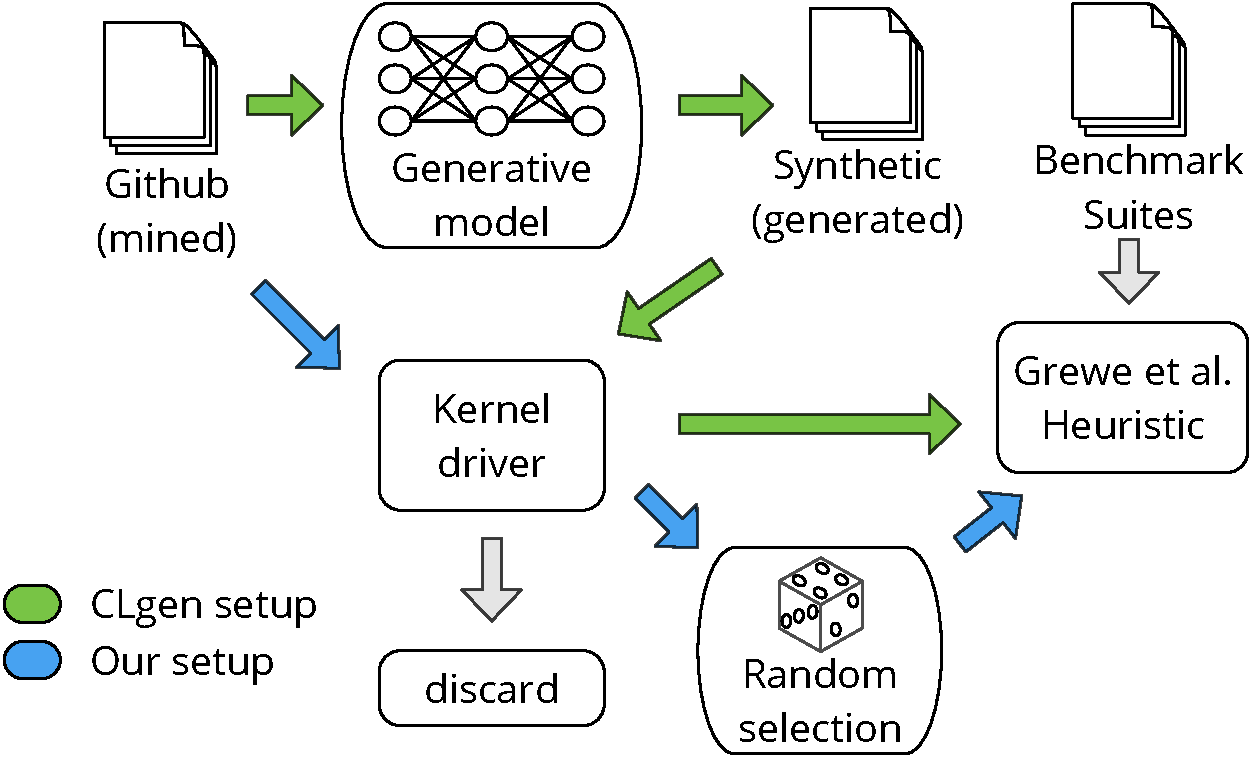
\includegraphics[width=.8\textwidth]{figures/clgen_flow.pdf}
	\caption{The flow of CLGen and our re-evaluation. Reproduced from Figure~1 in~\cite{goens_mapl19}.}
	\label{fig:clgen_flow}
\end{figure*}

We investigated these problems in~\cite{goens_mapl19}, where we re-evaluated the benchmark generation of CLGen~\cite{cummins_cgo17}.
Figure~\ref{fig:clgen_flow} summarizes the flow of CLGen and our re-evaluation.
In the original CLGen setup, the authors of~\cite{cumins_cgo17} mined kernels from Github to train a generative model of code.
The model in CLGen was a character-based model using a \ac{LSTM}\cite{lstm} architecture to learn a character distribution from (normalized) code.
The generative model is then used to generate synthetic benchmarks. A driver ensures they compile and provides input values for the generated benchmarks, which are used together with a set of established benchmark suites to train a heuristic.
The Grewe et al. heuristic~\cite{grewe_cgo2013} trained from these benchmarks is a machine learning model that decides based on a set of hand-designed code features whether to execute an OpenCL kernel in a \acsu{CPU} or the \acsu{GPU}. 
Our setup~\cite{goens_mapl19} takes the alternative route of foregoing the generative model, and using the mined github kernels instead of the synthetic benchmarks.

\begin{figure}[h]
	\centering
\resizebox{0.95\textwidth}{!}{
     \input{generated/clgen_accuracy}
     }
   \caption{Accuracy obtained by the heuristic for the different datasets in the setup. Adapted from Figure~2 of~\cite{goens_mapl19}.}
   \label{fig:clgen_accuracy}
\end{figure}

Figure~\ref{fig:clgen_accuracy} shows box plots comparing the accuracy obtained by the heuristic using the different datasets in both scenarios.
In all cases, one of the benchmarks was excluded from the training dataset and used as test set. We repeated the experiment for all benchmark suites as test set.
For the Github dataset we select a subset of the same size ($1000$) as the CLGen dataset used, which is part of the artifact of~\cite{cummins_cgo17}.
We repeat a random selection of a subset of the Github data $100$ times and report the median accuracy obtained this way, to control for the size of the dataset.
We also consider both the enhanced datasets as in the original work~\cite{cummins_cgo17}, namely the benchmarks enhanced with the CLGen kernels and alternatively enhanced by the original mined Github kernels.
Finally we also consider using each dataset on its own for training, to help the comparison between the usefulness of the Github kernels and the generated CLGen kernels. 
It is obvious that the kernels generated by CLGen are not as useful for training as are the original Github kernels.
We also empirically showed that adding more kernels did not help (see~\cite{goens_mapl19}).
We believe the problem is that the generated kernels are not \emph{representative}.
They are not as useful for maximizing $E[\mathcal{P}]$ as outlined above, $\mathcal{P}$ being the accuracy of the \ac{CPU}/\ac{GPU} mapping.
We have to be careful with the conclusions we can draw from this.
Particularly, upon closer examination (see~\cite{goens_mapl19}), the feature space of the Grewe et al~\cite{grewe_cgo2013} heuristic seems to be rather ill-suited for the task.

\begin{figure}[h]
	\centering
\resizebox{0.95\textwidth}{!}{
     \input{generated/clgen_pca}
     }
   \caption{Smoothed relative frequencies of kernels as function of the first principal component. Adapted from Figure~6 of~\cite{goens_mapl19}.}
   \label{fig:clgen_pca}
\end{figure}

Figure~\ref{fig:clgen_pca} shows a smoothed estimation of the relative frequencies of kernels. The feature space is obviously not one-dimensional. We thus project it into one dimension for visualization by making a principal component analysis using all points.
The figure shows the relative frequencies as a function of the first principal component, i.e. the one with the largest eigenvalue (by modulus). 
This figure thus serves to reproduce the intuition of representativeness as illustrated in Figure~\ref{fig:histograms}.
It is very clear that the (feature) space covered by the benchmarks is larger than that covered by the Github kernels. These, in turn, cover more of the feature space than the generated CLGen kernels.
This results are a consistent with an explanation of the results from Figure~\cite{fig:clgen_acuracy} within the formalism as introduced here.
Concretely, considering the formalism of benchmarks as reproducing a particular probability density and considering the task we want to learn as a random variable.
We believe this probabilistic model of benchmarks has the potential to drive research forward in this direction, and we should focus on it in future work.

A clear first conclusion from this re-thinking of the benchmarking model is that we should also question the objective we are measuring in Figure~\ref{fig:clgen_accuracy}.
The accuracy we consider is the accuracy on the established benchmark suites.
While this seems natural, the question is, is it the most useful objective?
In a real-world scenario we will have our own codebase and will want to get the maximal accuracy in our code base.
Good performance in the benchmarks is only useful to us if our code is similar to that on the benchmarks. 

To evaluate this scenario, we took all kernels $91$ from a concrete project, the Freedesktop project\footnote{https://www.freedesktop.org/}, and removed them form the Github dataset.
The choice of the project is arbitrary, the important property being that it has a moderate amount of kernels without significantly reducing the Github dataset to the point we cannot use it.
Using the same methods as above, we assessed the accuracy of training with all seven\footnote{the benchmark suites are: AMD SDK, NPB, NVIDIA SDK, Parboil, Polybench, Rodinia, SHOC} benchmark suites compared to the Github kernels, without the Freedesktop kernels, obviously.
Surprisingly, the heuristic performed significantly better with the Github kernels at $73\%$, compared to the $48\%$ obtained with the established benchmarks.
These results support the thesis that the concept of representativeness is central to benchmarking and models like the one proposed here should be investigated more.

\subsection{Models of Code}

One property of the generative models in CLGen is the way they represent code.
They do so by considering the (normalized) code as a stream of characters that the model learns to predict.
So far in this thesis we have strongly motivated graph-based representations of code, from the dataflow graphs even to the closely-related level graphs.
It is certainly not a new insight that graphs are well-suited to represent code in its non-linearity.
Compiler construction in general is based on multiple graphs, like the syntax trees or \acp{CDFG}.

Based on this we investigated graph-based representations of code for machine learning, specifically focusing on compilers~\cite{brauckman_cc20}.
Graph models in machine learning are an emerging field, with \acp{GNN}~\cite{gnn} being successful in multiple reasoning tasks.
In the context of programming language models, \acp{GNN} have also been very successful~\cite{allamanis2017learning,cummins_programl,ye2020deep,paliwal2020graph}.
These models use a iterative message-passing semantics to learn the dependencies from adjacent nodes in a graph. 
We designed code representations based on two graph representations of code common in compilers~\cite{brauckmann_cc20}, \acp{CDFG} and \acp{AST}, as well as a general framework for investigating these kinds of code representations~\cite{brauckmann_fdl20}.
Details about the machine learning architecture are beyond the scope of this thesis, here we just discuss the graph-based models and how they expose their semantics.

\begin{figure}[h]
	\centering
\resizebox{0.95\textwidth}{!}{
     \input{generated/graph_representations_code}
     }
   \caption{A comparison of the accuracy of multiple machine learning methods for the \ac{CPU}/\ac{GPU} classification of OpenCL kernels. Adapted from Figure~12 of~\cite{brauckman_cc20}.}
   \label{fig:graph_representations_code}
\end{figure}

To test the different compiler-based graph representations of code, we trained~\cite{brauckman_cc20} multiple deep learning models for the OpenCL \ac{CPU}/\ac{GPU} classification task described above.
Figure~\ref{fig:graph_representations_code} shows a comparison of the accuracy of the different graph-based models.
The baseline model by Grewe et al.~\cite{grewe_cgo2013} is the same baseline model from above.
Additionally, we compare with two state-of-the-art deep learning models for this task, DeepTune~\cite{cummins_pact17} and inst2vec~\cite{inst2vec}.
The graph-based models we evaluate are a control flow graph (CFG), and \acf{CDFG}, enhanced with multiple edge annotations, for data dependencies of the return values of function calls (CALL) and store-load memory dependencies (MEM).

The graph shows two distinct evaluation setups.
The first is the random split setup, which is the same one used by~\cite{cummins_pact17,benun_neurips18}.
It joins all seven benchmark suites investigated into a large set of kernels and randomly splits it into $10$ disjoint subsets.
Each of the disjoint subsets is then used as the testing set, training with all other nine.
We report the geometric means of the accuracy~\cite{fleming1986gmean}.

A potential problem with the random split setup is that it mixes kernels from the same benchmark, which are likely to be more similar. 
This goes back to the representativeness argument for the Freedesktop evaluation above.
A random split assumes a more representative benchmark for training.
To investigate how this affects the algorithms, we change the split to also test how they generalize across benchmark suites.
Instead of random disjoint subsets of equal sizes, we split the kernels for test/training according to the benchmark suites.
One suite is used for testing, all others for training, and we again report the geometric mean of the accuracy.
This is the second setup, the grouped split.

The results in Figure~\ref{fig:graph_representations_code} show that graph-based models generally achieved better accuracy than sequence-based ones.
This is not surprising, as it has been discussed that they are better at exposing the non-linear structure of code.
Also not surprising is that all models do worse in the grouped split, when forced to generalize across benchmark suites.
However, it is worth noting that the \ac{CDFG}-based representations performed better on the random split, and the \ac{AST}-based representations performed better on the grouped split.
A \ac{CDFG} is at a level of abstraction closer to the machine than an \ac{AST}, which is closer to the code itself as written by a human.
In this light, it is not surprising that a \ac{CDFG}-based representation was better at learning with a more representative benchmark in the random split.
The problem in that case is more related to the execution of code on a \ac{CPU} or a \ac{GPU}, whereas on the grouped split, understanding the semantics of the code is more important for predicting how it might fare.

In this section we have seen how graph-based representations and the level of abstraction are important, as well as how we should pay closer attention to the representativeness of a benchmark.
A natural question at this stage is whether this insight can be used to improve generative models and generate better, more representative benchmarks.
For this we also need graph-based generative models, which have received less attention than \acp{GNN} in inference.
The graph generative model of~\cite{li2018learning} that works by generating sequences that construct the graph.
While this allows us to create graphs representing code, the sequential structure of the generative sequences still pose some problems.
This model is also very generic, which it easy to generate invalid code graphs, just the same that CLGen can generate invalid code.
In his Diploma Thesis, which I supervised, Alexander Brauckmann managed to generate more valid code samples than CLGen~\cite{Brauckmann-diplom20} (up to 88\%, compared to 38\% for CLGen).
In a related effort, Alexander Thierfelder designed a domain-specific extension to the model of~\cite{li2018learning}, aiming to generate LLVM-based graphs that are correct by construction~\cite{Thierfelder-master20}.
The LLVM language is complex, and we could unfortunately not design a generative model where the graphs are correct by construction, but we could capture most of the LLVM semantics in the model.
Graph-based models of code are a promising direction for future work, which could allow us to generate representative benchmarks, among others~\cite{leather_fdl20}. %mapl, cc20


\chapter{Mathematical Structures in Mappings}
\label{chap:mapping_structures}
The space of mappings in the software synthesis flow we described has a rich mathematical structure.
This chapter aims to explore and expose that structure, at least in part.
We will consider two main aspects of the mathematical structure hidden within the simple notion of a mapping, namely the inherent symmetry, and the degrees of similarity between mappings.
We will consider how to extract this structure in a computationally-efficient fashion, and how it can be exposed to tools that aim to exploit it, in different representations.

This thesis focuses primarily on a view of the mapping problem centered on computation, instead of data.
In many cases, with the increasing discrepancy between execution frequency and memory access times (cf. Figure~\ref{fig:multicore_era}) this view is not ideal.
The problem space of data allocation is usually more clearly structured and can be modeled better. 
For example, we worked on \ac{ILP}-based methods to describe and optimize memory allocation~\cite{odendahl_date14,odendahl15,goens_jsa16}.\index{\acl{ILP}}
We omit this work from this thesis for space reasons, to keep the scope manageable.

We also omit work on emerging memory technologies, concretely \ac{RTM}, where we used similar \ac{ILP}-based models and other meta-heuristics like genetic algorithms or domain-specific heuristics to optimize data placement~\cite{khan_date20}.\index{\acl{RTM}}\index{emerging memory technologies}

\section{Symmetries}
\label{sec:symmetries}
In this chapter we will explore the mathematical structure of symmetry in the software synthesis process, mostly the work published in ~\cite{goens_iess15,goens_taco17,goens_scopes17,goens_mcsoc18,goens_tcad21}.
The material in this section makes use of concepts in group theory.
We assume the basic concepts as seen in any undergraduate course on group
theory, with the definitions of groups, actions and orbits.
A brief introduction, to the level required by this chapter, can be found in Appendix~\ref{appendix:groups}. 

\subsection{Architectures and Applications}
\label{sec:arch_app_symmetries}

Intuitively, when we say an object is very symmetric we usually mean it has parts that are similar or identic, and the object looks identical (or similar) from multiple points of view.
In a symmetric face, for example, both the left and right sides of the face are similar. A hexagonal mosaic might look the same when seen from six different angles.
Mathematically, this is commonly modeled through transformations. A reflection along the vertical axis in a face, or rotations of $60^\circ$ in the heaxgon, both leave the object (mostly) unchanged.
We can do the same for hardware architectures, even heterogeneous ones.

For example, the Exynos~5 in the Odroid-XU4 has four identical Cortex A7\texttrademark, say $\PE_1,\ldots,\PE_4$ and four identical Cortex A15\texttrademark cores, say $\PE_5,\ldots,\PE_8$.
A transformation that swaps the cores $\PE_1$ and $\PE_2$ leaves the archtiecture topology unchanged, since the cores are identical. This is depicted in Figure~\ref{fig:exynos_symmetries}.
On the other hand, a transformation that swaps $\PE_1$ and $\PE_5$ does change the topology, since the cores are of different types. As can also be seen in Figure~\ref{fig:exynos_symmetries}.
\begin{figure}[h]
	\centering
\resizebox{0.3\textwidth}{!}{
   \begin{tikzpicture}
     %little cores
\node (pe1) at ({-1.5},{4}) [draw,minimum width=2.5cm,align=center,minimum height=2cm, fill=green!30] {\huge PE$_1$};
\node (L1-pe1) at (-1.5,2.5) [draw,minimum width=2.5cm,align=center,minimum height=1.5cm, fill=blue!30] {\huge L1\$};
\node (pe2) at (-1.5+3,4) [draw,minimum width=2.5cm,align=center,minimum height=2cm, fill=green!30] {\huge PE$_2$};
\node (L1-pe2) at (-1.5+3,2.5) [draw,minimum width=2.5cm,align=center,minimum height=1.5cm, fill=blue!30] {\huge L1\$};
\node (pe3) at (-1.5,4+4) [draw,minimum width=2.5cm,align=center,minimum height=2cm, fill=green!30] {\huge PE$_3$};
\node (L1-pe3) at (-1.5,2.5+4) [draw,minimum width=2.5cm,align=center,minimum height=1.5cm, fill=blue!30] {\huge L1\$};
\node (pe4) at (-1.5+3,4+4) [draw,minimum width=2.5cm,align=center,minimum height=2cm, fill=green!30] {\huge PE$_4$};
\node (L1-pe4) at (-1.5+3,2.5+4) [draw,minimum width=2.5cm,align=center,minimum height=1.5cm, fill=blue!30] {\huge L1\$};

%big cores
\node (pe5) at ({6.5-1.5},{4}) [draw,minimum width=2.5cm,align=center,minimum height=2cm, fill=green!60] {\huge PE$_5$};
\node (L1-pe5) at (6.5-1.5,2.5) [draw,minimum width=2.5cm,align=center,minimum height=1.5cm, fill=blue!30] {\huge L1\$};
\node (pe6) at (6.5-1.5+3,4) [draw,minimum width=2.5cm,align=center,minimum height=2cm, fill=green!60] {\huge PE$_6$};
\node (L1-pe6) at (6.5-1.5+3,2.5) [draw,minimum width=2.5cm,align=center,minimum height=1.5cm, fill=blue!30] {\huge L1\$};
\node (pe7) at (6.5-1.5,4+4) [draw,minimum width=2.5cm,align=center,minimum height=2cm, fill=green!60] {\huge PE$_7$};
\node (L1-pe7) at (6.5-1.5,2.5+4) [draw,minimum width=2.5cm,align=center,minimum height=1.5cm, fill=blue!30] {\huge L1\$};
\node (pe8) at (6.5-1.5+3,4+4) [draw,minimum width=2.5cm,align=center,minimum height=2cm, fill=green!60] {\huge PE$_8$};
\node (L1-pe8) at (6.5-1.5+3,2.5+4) [draw,minimum width=2.5cm,align=center,minimum height=1.5cm, fill=blue!30] {\huge L1\$};


\node (L2-little) at (0,0) [draw,minimum width=6cm,align=center,minimum height=1.5cm, fill=blue!55] {\huge L2\$};
\node (L2-big) at (6.5,0) [draw,minimum width=6cm,align=center,minimum height=1.5cm, fill=blue!55] {\huge L2\$};
\node (DRAM) at (3.25,-2.5) [minimum width=12.5cm,align=center,minimum height=2cm, fill=blue!85] {\huge DRAM};
   \end{tikzpicture}
 }
   \caption{Symmetries in the Odroid-XU4 architecture. TODO: fix figure.}
   \label{fig:exynos_symmetries}
\end{figure}

When the memory subsystem is more complex, this is also reflected in the topology. Consider the \ac{NoC}-based architecture depicted in the example, with four identical cores $\PE_1\ldots,\PE_4$.
An analogous transformation to the one described before, which swaps the cores $\PE_1$ and $\PE_2$, is not a symmetry of this topology, as depicted in Figure~\ref{fig:non_equivalent}.
The change in the cores changes the communication patterns.
Before the transformation, sending data from $\PE_1$ to $\PE_3$ needs two hops over the \ac{NoC}, whereas after the transformation it can be sent within a single hop.

\begin{figure}[h]
	\centering
\resizebox{0.3\textwidth}{!}{
   \begin{tikzpicture}
     %little cores
\node (pe1) at ({-1.5},{4}) [draw,minimum width=2.5cm,align=center,minimum height=2cm, fill=green!30] {\huge PE$_1$};
\node (L1-pe1) at (-1.5,2.5) [draw,minimum width=2.5cm,align=center,minimum height=1.5cm, fill=blue!30] {\huge L1\$};
\node (pe2) at (-1.5+3,4) [draw,minimum width=2.5cm,align=center,minimum height=2cm, fill=green!30] {\huge PE$_2$};
\node (L1-pe2) at (-1.5+3,2.5) [draw,minimum width=2.5cm,align=center,minimum height=1.5cm, fill=blue!30] {\huge L1\$};
\node (pe3) at (-1.5,4+4) [draw,minimum width=2.5cm,align=center,minimum height=2cm, fill=green!30] {\huge PE$_3$};
\node (L1-pe3) at (-1.5,2.5+4) [draw,minimum width=2.5cm,align=center,minimum height=1.5cm, fill=blue!30] {\huge L1\$};
\node (pe4) at (-1.5+3,4+4) [draw,minimum width=2.5cm,align=center,minimum height=2cm, fill=green!30] {\huge PE$_4$};
\node (L1-pe4) at (-1.5+3,2.5+4) [draw,minimum width=2.5cm,align=center,minimum height=1.5cm, fill=blue!30] {\huge L1\$};

%big cores
\node (pe5) at ({6.5-1.5},{4}) [draw,minimum width=2.5cm,align=center,minimum height=2cm, fill=green!60] {\huge PE$_5$};
\node (L1-pe5) at (6.5-1.5,2.5) [draw,minimum width=2.5cm,align=center,minimum height=1.5cm, fill=blue!30] {\huge L1\$};
\node (pe6) at (6.5-1.5+3,4) [draw,minimum width=2.5cm,align=center,minimum height=2cm, fill=green!60] {\huge PE$_6$};
\node (L1-pe6) at (6.5-1.5+3,2.5) [draw,minimum width=2.5cm,align=center,minimum height=1.5cm, fill=blue!30] {\huge L1\$};
\node (pe7) at (6.5-1.5,4+4) [draw,minimum width=2.5cm,align=center,minimum height=2cm, fill=green!60] {\huge PE$_7$};
\node (L1-pe7) at (6.5-1.5,2.5+4) [draw,minimum width=2.5cm,align=center,minimum height=1.5cm, fill=blue!30] {\huge L1\$};
\node (pe8) at (6.5-1.5+3,4+4) [draw,minimum width=2.5cm,align=center,minimum height=2cm, fill=green!60] {\huge PE$_8$};
\node (L1-pe8) at (6.5-1.5+3,2.5+4) [draw,minimum width=2.5cm,align=center,minimum height=1.5cm, fill=blue!30] {\huge L1\$};


\node (L2-little) at (0,0) [draw,minimum width=6cm,align=center,minimum height=1.5cm, fill=blue!55] {\huge L2\$};
\node (L2-big) at (6.5,0) [draw,minimum width=6cm,align=center,minimum height=1.5cm, fill=blue!55] {\huge L2\$};
\node (DRAM) at (3.25,-2.5) [minimum width=12.5cm,align=center,minimum height=2cm, fill=blue!85] {\huge DRAM};
   \end{tikzpicture}
 }
   \caption{The communication topology affects symmetries in architectures.}
   \label{fig:non_equivalent}
\end{figure}

Generally, the transformations that preserve the structure of the architecture topology have a clear structure.
If two transformations $t_1$ and $t_2$ preserve the structure of the architecture topology, then their composition $t_1 \circ t_2$ also preserves it.
Similarly, it is clear that reversing a transformation $t_1^{-1}$ also preserves the structure.
Finally, the identity transformation on the architecture $\operatorname{id}_A$ (which does not change anything) clearly preserves the structure.
These observations together mean that these transformations have the structure of a group with the function composition $(\circ)$ as its operation.

More precisely, the group of symmetries of the achitecture is precisely the group of graph isomorphisms from the architecture graph $A$ to itself.
An isomorphism from an object to itself is called an automorphism\index{automorphism}.
We denote the group of automorphisms of the architecture $A$ as $\Aut(A)$

For the case of the \ac{NoC}-based architecture, the authomorphism group $\Aut(A\text{NoC}) \cong D_4$ is a dihederal group on $4$ points.
It conists of $3$ rotations, $4$ reflections and the identity transformation.
The Odroid architecture, on the other hand, has $\Aut(A_\text{Odroid}) \cong S_4 \times S_4$ as symmetry group.
This group with $48$ transformations is comprised of (independent) arbitrary permutations of the A15 and A7 cores.

Since the Odroid architecture is heterogeneous, both clusters are distinct and there is no symmetry between them.
Many complex architectures, however, do consist of multiple identical culsters. Consider the architecture depicted in Figure~\ref{fig:coolidge}.
It is the MPPA3 Coolidge from Kalray~\cite{coolidge} and consists of $5$ identical clusters.
Each cluster has $17$ cores, $16$ of which are identical general-purpose cores, and the last one is a special-purpose secure and management core.

The MPPA3 Coolidge is a hierarchically-designed architecture. The five identical clusters are conceptually at a different level than the cores at each cluster.
Designs like the HAEC~\cite{HAEC} topology mentioned in the introduction (cf. Figure~\ref{fig:haec}) have even more levels of hierarchy.
The symmetries of these hierarchical architectures are reflected in the different levels of hierarchy of the topology~\cite{goens_tcad21}.
For example, the automorphism group of the MPPA3 Coolidge is $\Aut(A_\text{Coolidge}) \cong S_{16} \wr S_5$ and has $16! \cdot 5! \approx 2.51 \cdot 10^{15}$ symmetries. 

So far we have discussed the symmetries of architectures.
However, we can apply the same principle to applications and their graphs.
Conisder the audio filter example application from Section~\ref{sec:kpn_basic} (cf. Figure~\ref{fig:audio_filter_graph}). 
The left and right channels perform precisely the same computation on different data.
We could not, for example, just swap the \texttt{fft\_l} and \texttt{fft\_r} nodes, since that would result in a different application that also swaps the channels of the audio file.
On the other hand, if we swap the whole subgraph consisting of \texttt{fft\_l}, \texttt{filter\_l} and \texttt{ifft\_l} with the equivalent subgraph of \texttt{fft\_r}, \texttt{filter\_r} and \texttt{ifft\_r}, the application remains identical.
This is depicted on Figure~\ref{fig:audio_filter_symmetries}.

\begin{figure}[h]
	\centering
\resizebox{0.9\textwidth}{!}{
\begin{tikzpicture}
   \node[draw, ellipse,minimum width = 1.1cm, minimum height=0.9cm] (src) {src};
\node[draw, ellipse,minimum width = 1.1cm, minimum height=0.9cm, below right = 1cm of src] (fft_l) {\texttt{fft\_l}};
\node[draw, ellipse,minimum width = 1.1cm, minimum height=0.9cm, above right = 1cm of src] (fft_r) {\texttt{fft\_r}};
\node[draw, ellipse,minimum width = 1.1cm, minimum height=0.9cm, right = 1 cm of fft_l] (filter_l) {\texttt{filter\_l}};
\node[draw, ellipse,minimum width = 1.1cm, minimum height=0.9cm, right = 1 cm of fft_r] (filter_r) {\texttt{filter\_r}};
\node[draw, ellipse,minimum width = 1.1cm, minimum height=0.9cm, right = 1 cm of filter_l] (ifft_l) {\texttt{ifft\_l}};
\node[draw, ellipse,minimum width = 1.1cm, minimum height=0.9cm, right = 1 cm of filter_r] (ifft_r) {\texttt{ifft\_r}};
\node[draw, ellipse,minimum width = 1.1cm, minimum height=0.9cm, below right = 1cm of ifft_r] (sink) {\texttt{sink}};

\draw[-latex] (src) -- (fft_l);
\draw[-latex] (src) -- (fft_r);
\draw[-latex] (fft_l) -- (filter_l);
\draw[-latex] (fft_r) -- (filter_r);
\draw[-latex] (filter_l) -- (ifft_l);
\draw[-latex] (filter_r) -- (ifft_r);
\draw[-latex] (ifft_l) -- (sink);
\draw[-latex] (ifft_r) -- (sink);
 \end{tikzpicture}
}
   \caption{A symmetry of the audio filter application. TODO: adapt figure}
	\label{fig:audio_filter_symmetries}
\end{figure}

Mathematically, we need to model the semantics of the application to reflect its symmetries.
For an application $K = (V_K,E_K)$ we can label the nodes $V_K$ with unique identifiers relating them to the $KPN$ process that execute them (e.g. the \texttt{\_\_PNprocess} in a \ac{CPN} program). 
Formally, thus, the automorphism group $\Aut(E)$ of the labeled graph $K$ is trivial, i.e. $\Aut(E) = \{ \id \}$. 
We could label $K$ differently to capture the symmetry from Figure~\ref{fig:audio_filter_symmetries}.
For example, if use the source code of the process as label, we would capture this symmetry.
We have to be more careful, however, as this can lead to a problematic definition of symmetries.

An application might use the same code at different points, resulting in very different behavior.
For example, consider an application that receives a list of points, which it sorts before operating on it.
Before returning the list, it sorts them again to ensure they are sorted.
Both times it sorts the list using the quicksort algorithm, yet the second time the list is almost always sorted or close to being sorted.
Then the execution of the same quicksort code in the second instance behaves very differently from the first time.

A difference like the one outlined above is very difficult to capture automatically, as it requires understanding of the application to a very high level of abstraction.
We thus consider application symmerties as manually-defined anotations.
There are some conceivable ways to automatically capture and annotate such application symmetries, for example when dealing with known data-level parallelism.
In future work, a framework as we discuss in Chapter~\ref{chap:mocs}, Section~\ref{sec:macqueen} could be extended to extract symmetries.
For the rest of this thesis, however, we focus on symmetries induced from the architecture.

\subsection{Mappings}

We have seen how the architecture and applications have symmetries in their structure. 
The groups $\Aut(A)$ and $\Aut(K)$ act on the architecture $A$ and the application $K$, respectively.
These actions also induce an action on the mapping space. 
Let $m : K \rightarrow A$ be a mapping.
Recall that a symmetry $\sigma \in \Aut(A)$ of the architecture is a transformation that leaves the structure of the architecture unchanged.
Conisder then the mapping $\sigma m := k \mapsto \sigma(m(k))$.
Since the structure of $A$ is unchanged, then the structure of $m$ and $\sigma m$ is also identical.
All observable properties of $m$ and $\sigma m$, like the execution time or energy consumption, are the same.
If they were not, it would have to be due to a structural difference in the (sub)architectures $m(K),(\sigma m)(k) = \sigma(m(K)) \leq A$, which are isomorphic by assumption on $\sigma$.
We say that these properties like the execution time and energy consumption are \emph{invariants}\index{invariants} of the group action.

Figure~\ref{fig:mapping_action_example} shows an example of the action on mappings. \todo{add and describe figure.}

The case for $K$ is analogous.
Let $\pi \in \Aut(K)$ be a symmetry of the application.
Then the mapping $\pi m := k \mapsto m(\pi^{-1}k)$ is equivalent to $m$.
Note that we define it with $\pi^{-1}$ instead of $\pi$ so that this defines a left action.
Indeed, for $\pi, \tau \in \Aut(K)$, we have
\begin{align*}
  (\pi (\tau m))(k) = \pi m(\tau^{-1}k) = m(\pi^{-1}\tau^{-1}k) = m((\tau \pi)^{-1}k) = ((\tau \pi) m))(k) 
\end{align*}

From the models of the problem, as defined in Chapter~\ref{chap:mapping}, mappings under these symmetries are necessarily indistinguishable from each other, since they rely on inherent symmetries of the models.
On the other hand, these are just models, they need not reflect reality.
It still leaves the question open, how does this hold up in pracitice?
Are equivalent mappings actually equivalent?
In~\cite{goens_scopes17} we tested this empirically, by executing four equivalent mappings and measuring the runtime and energy.
We tested four equivalent mappings of the audio filter benchmark on an Odroid XU3 and executed each $50$ times, measuring three metrics.
The Odroid XU3 is almost identical to the Odroid XU4, but features on-board energy sensors.
We measured the \acs{CPU} time, which is the total aggregate time spent by all \acsp{CPU} executing the application.
We also measured the wall-clock time, which is the total time of the application, measured from start to finish as it would pass on a wall clock.
Finaly, we measured the total energy over the INA-231 sensors connected over the I2C bus, as the aggregate of the energy measured at each individual component, sampled at $10$~Hz.

\begin{figure}[h]
	\centering
\resizebox{0.95\textwidth}{!}{
     \input{generated/mappings_equivalent}
 }
   \caption{Measurements of four equivalent mapings for the audio filter application on the Odroid-XU3 architecture.}
   \label{fig:symmetry_measurements}
\end{figure}

Figure~\ref{fig:symmetry_measurements} shows the results of the measurements as box-and-whiskers plots.
We see that the execution times of all mappings are well within the ranges of each other, both when measured as wall-clock or \ac{CPU} time.
We can test this in a more rigurous fashion with an \ac{ANOVA} F-test.
For the wall-clock data, we get a probability of $p = 5.06\%$, rejecting the null hypothesis that variance in the wall-clock times from different mappings is explained by more than statistical variance.
For the \ac{CPU} time data, the value of $p=15.2\%$ it is even clearer that the variance is likely just statistical.
We can conclude that, at least for this example, equivalent mappings indeed seem to have the same execution time behavior.

The energies of the mappings are less clearly distinct, especially for the first two mappings, yet they all still require comparable amounts of erengy.
An \ac{ANOVA} F-test yields a $p$ value of $0.009\%$.
It is worth noting here that these measurements are just a first estimation.
The accuracy of the energy data depends on a multitude of factors like the sampling rate or the measurement accuracy of the INA-231 sensors.
We have not made a proper assesment of measurement errors and error propagation, which is especially large in the energy measurements that span measurements from four different components.
Precise energy measurments, however, are beyond the scope of this thesis.
We this experiment we cannot really conclude nor discard the hypothesis that energy consumption is an invariant of the mapping symmetries.

\subsection{Calculating Symmetries}

The branch of mathematics known as computational group theory deals with computational aspects of the theory of groups, which we have used here for formalizing the symmetries of applications, architectures and mappings. 
An overview of the methods of computational group theory can be found in~\cite{holt,seress2003permutation}, which both cover far beyond the basics presented in this subsection.
Here we will present only the methods necessary for the calculations required of applications to software synthesis.

To leverage the symmetries explained in this theses for software synthesis, we need to methods to calculate the following:
\begin{enumerate}
\item\label{prob:autgrp} Given an architecture graph $A$, the group of symmetries $\Aut(A)$.
\item\label{prob:orbit} Given a mapping $m : T \rightarrow A$ and the symmetry group $G := \Aut(T \rightarrow A)$, enumerate the orbit $Gm$.
\item\label{prob:equiv} Given two mappings $m,m' : T \rightarrow A$ and the symmetry group $G := \Aut(T \rightarrow A)$, determine whether $m = gm'$ for a $g \in G$, i.e. if the two mappings are in the same orbit.
\end{enumerate}

Mature software exists for computational group theory that can, in principle, solve these problems. 
The \acs{GAP} system is a \ac{DSL} for computational discrete algebra with a focus on (computational) group theory~\cite{gap}.
We developed algorithms for dealing with problems \ref{prob:autgrp}-\ref{prob:equiv} in \ac{GAP}~\cite{goens_taco17}.
We also included naive versions of most algorithms implemented directly in Python in \mocasin.

Using \ac{GAP}-based algorithms in software synthesis tools like \ac{MAPS} in practice, however, comes with a series of complications.
The largest problem is that it adds a dependency on a whole ecosystem.
A complete distribution of \ac{GAP} is over $200$ MiB of size and takes around a second to start up in standard commodity hardware of today.
Additionally, to communicate with a running \ac{GAP} instance we need to use \ac{POSIX} pipes, which is cumbersome and not portable.
A project existed to use \ac{GAP} as a library, but seems to be unmaintained, and we could not get it to function.
We thus developed a standalone library~\cite{nicolai_studienarbeit}, \mpsym , which implements the required algorithms to solve problems ~\ref{prob:autgrp}-\ref{prob:equiv} and includes a domain-specific extension for efficiently dealing with hierarchical (e.g. clustered) archictures~\cite{goens_tcad21}.

Calculating the group of symmetries from an architecture graph (Problem~\ref{prob:autgrp}) is very related to the graph isomorphism problem. 
This is a problem in NP, and it is not known, neither believed to be in P nor NP-complete. 
In December 2015, L\'{a}sl\'{o} Babai published a pre-print where he claims to have found a quasi-polynomial algorithm~\cite{babai_graph_isomorphism}, 
yet at the time of this writing (January 2021) the peer-review is still not complete.
Regardless of the worst-case complexity, graph isomorphism can be solved efficiently in practice for most instances~\cite{McKay201493}.
Algorithms for doing so are implemented in nauty/Traces, which \mocasin and \mpsym use to solve Problem~\ref{prob:autgrp}.

Most algorithms in computational group theory use a special data structure describing the group.
This data structure is called a \emph{\ac{BSGS}}, see~\cite{holt,seress2003permutation} for more details.\index{base and strong generating set}
The standard algorithm for calculating the \ac{BSGS} for a group is the Schreier-Sims Algorithm\index{Schreier-Sims Algorithm}.
Multiple variants of this algorithm exist, which are more efficient under different circumstances.
\acp{CAS} like \ac{GAP} use different variants with sophisticated heuristics for selecting which variant to use.
In \mpsym we implement some variants of the Schreier-Sims with less sophisticated selection, which do not surpass \ac{GAP}'s performance.
For all groups investigated in this thesis, however, \mpsym was comparable to \ac{GAP}, without the large ecosystem dependency~\cite{nicolai_studienarbeit,goens_tcad21}.

Problem~\ref{prob:orbit} is a standard problem in computational group theory.
We solve it using the Orbit algorithm, which can easily be adapted to a lazy variant, described in Algorithm~\ref{label:algo:lazy_orbit}.
If we use a perfect hash, the algorithm returns exactly the orbit of the mapping.
If the hash can have duplicates, a smaller orbit might be returned, but the algorithm will clearly never yield elements from outside the orbit.
This lazy variant is especially useful when looking for any mapping in the orbit which fullfils some properties, instead of being interested in the full orbit.
This is especially useful in the \acs*{TETRiS} system, which we will describe in Section~\ref{sec:tetris}.

\begin{algorithm}
	\caption{A lazy variant of the standard orbit algorithm}
	\label{algo:lazy_orbit}
	\begin{algorithmic}[1]
	  \Input{A generating set $X = (g_1, \ldots, g_n), \langle g_1, \ldots, g_n \rangle = \operatorname{AutGrp}(M)$ for the mapping space, a mapping $m_0$. }
	  \Output{The orbit of $m_0$: $\operatorname{AutGrp}(M)m = \{ g m_0 \mid g \in \operatorname{AutGrp}(M) \}$ }
     \State H $\leftarrow$ $\{ \operatorname{Hash}(m_0) \}$
     \State CurElems $\leftarrow$ $\{ g_i m_0,~\operatorname{Hash}(g_i m_0) \notin H \mid i = 1,\ldots,n \}$
     \State H $\leftarrow$ $H \cup \{ \operatorname{Hash}(m) \mid m \in \text{CurElems} \}$
     \While{ CurElems $\neq \emptyset$}
	     \For{ $m \in \text{CurElems}$}
		         \State \textbf{yield }$m$
	     \EndFor 
     \State CurElems $\leftarrow$ $\{ g_i m,~\operatorname{Hash}(g_i m) \notin H \mid m \in \text{CurElems}, i = 1,\ldots,n \}$
     \State H $\leftarrow$ $H \cup \{ \operatorname{Hash}(m) \mid m \in \text{CurElems} \}$
   \EndWhile
	\end{algorithmic}
\end{algorithm}

Finally, to solve Problem~\ref{prob:equiv}, we could simply solve Problem~\ref{prob:orbit} for both elements and see if the orbits are identical.
Orbits form a partition of the mapping space $M$, meaning that two orbits are either identical or dijsoint (and the union of all orbits yields $M$).
This is a very inefficient way of solving Problem~\ref{prob:equiv}, since it means we have to enumerate the whole orbit for each element.
Using the same principle of the Orbit's partition, we can also just enumerate the orbit for one element and see if the other element is in it.
While this is also an improvement, it is still very inefficient. Orbits can be very large when the problem has much symmetry.
By default, \mpsym uses this variant as a fall-back method to solve Problem~\ref{prob:equiv} when correctness needs to be guaranteed.

Another alternative for this which works without enumerating any orbits is based on the fact that the symmetries of the mapping $\operatorname{AutGrp}(M) \leq \operatorname{Sym}(M)$, the symmetric group on $M$ (i.e. the group of all permutations on $M$).
Thus, if two mappings $m, m'$ are in the same orbit under $\operatorname{AutGrp}(M)$, then they are also in the same orbit under $\operatorname{Sym}(M)$: there exists a permutation $\sigma \in S_{|M|}$ which takes $m$ to $m'$.
However, $|M|$ as we have seen can be very large, as it grows (at least) as $|V_A|^|V_K|$ and $\operatorname{Sym}(M) \cong S_{|M|}$ is thus unimaginably large, namely $|\operatorname{Sym}(M)| = |M|! \geq (|V_A|^|V_K|)!$.
If we consider only architecture symmetries, this all works over the much smaller $\operatorname{AutGrp}(A)$.  We obviously do not have to iterate over the group to construct $\sigma$, since we know both $m,m'$ we can construct it directly.
Knowing $\sigma$, we can efficiently solve the \emph{group membership problem}~\cite{seress2003permutation} for these permutation groups, using the \ac{BSGS}. \index{group membership problem}
We know, namely, that $\sigma$ is in $\operatorname{AutGrp}(M)$ if and only if $\operatorname{AutGrp}(M)m = \operatorname{AutGrp}(M)m'$, by the definitions of the orbit and $\sigma$.
On the other hand, if we cannot construct $\sigma$ from $m,m'$, because it leads to contradictions, then, obviously, the orbits are different.

We did not implement this variant based on the group membership problem.
The reason for this is that we implemented an alternative which also allows us to select a mapping to work with, e.g. for \ac{DSE}.
It is based on canonical representatives~\cite{goens_taco17,goens_mcsoc18}.
A canonical representative of an orbit $Gm$ is an element $m_0 \in Gm$ such that there is a function
$f : G \setminus \setminus M \rightarrow M$ which maps $Gm$ to $m_0$.
In other words, the function $f$ selects a unique element of every orbit, this element is the canonical representative.

For constructing our canonical representatives, we order mappings using the \emph{lexicographical ordering}.
For two mappings $m = (m_1,m_2,\ldots,m_k), m' = (m'_1,\ldots,m'_k)$ we say that $m \leq m'$ if and only if there exists a $j \leq k$ such that $m_i = m'_i$ for all $i < j$ and $m_j \leq m'_j$.\index{lexicographical ordering}
The function $f$ for the canonical element of the orbit thus maps $Gm$ to $\min Gm$.
In other words, we choose canonical elements to be the lexicographical-minimal elements of the orbits.

\begin{algorithm}
   \caption{Local search for finding canonical representatives. Adapted from Algorithm~1 of~\cite{goens_mcsoc18}.}
   \label{algo:canonical_representatives}
   \begin{algorithmic}[1]
     \Input{A mapping $m$, a generating set $S$, with $\langle S \rangle = \operatorname{AutGrp}(M)$.}
     \Output{A mapping $m_\text{canonical} = gm$ with $m_\text{canonical} < m'$ for all $m' \in Gm$}
     \State $F \gets \{m\}$
     \State $F_\text{old} \gets \emptyset$
     \While {$F \neq F_\text{old}$}
     \State $F_\text{old} \gets F$
     \ForAll{ $s \in S$ }
     \ForAll{ $m' \in F$ }
     \If {$sm < m$}
     \State $F \gets sm$
     \EndIf
     \EndFor
     \EndFor
     \State \label{line:optional} \textbf{(optional)} $F \gets \{ \operatorname{min}_{ m' \in F} m' \}$
     \EndWhile
     \Return $\operatorname{min}_{ m' \in F} m'$
   \end{algorithmic}
 \end{algorithm}
 
To find the lex-minimal canonical representatives we use a local-search algorithm based on an iteration similar to the Orbit Algorithm. 
Algorithm~\ref{algo:canonical_representatives} shows this local-search heuristic. 
This algorithm to returns the lex-minimal element of the orbit if the generating set has a particular property, which we called being a \emph{strictly order-preserving generating set}~\cite{goens_mcsoc18}.
We say $S$ is a strictly order-preserving generating set if for two mappings $m' < m$ in the same orbit, i.e. $m \in \langle S \rangle m'$, there exists a word $s_1,\ldots,s_n$ in the generators $s_i \in S$, such that $m' = s_1 \ldots s_n m$ with $s_i (s_{i+1}\ldots s_n)m < (s_{i+1} \ldots s_n)m$ for all $i = 1,ldots,n-1$.\index{stricly order-preserving generating set}
For example, for the symmetric group $S_n$, the set of all transpositions $S = \{ (i,j) \mid i \neq j \in \{1,\ldots,n\} \}$ is such a strictly order-preserving generating set.
Without this property, the local search could yield an element which is not the lex-minimal element.
If we remove the optional reduction in Line~\ref{line:optional}, we significantly speed up this search and make the probability of finding only a local minimum instead of the global one higher.
Since all mappings in the orbit are equvialent, such a local minimum will always have the same objective properties $\Theta$ as the real canonical representative (cf. Section~\ref{sec:mapping_problem}).
Thus, finding a local minimum instead of the canonical representative is tantamount to considering a smaller group of symmetries, and thus a very acceptable risk for a considerable speed-up.
Both \mpsym and \mocasin implement this heuristic and use it by default for design-space exploration, as we will see in Section~\ref{sec:dse}. 
We also integrated \mpsym into \mocasin , using the simple Python versions of the algorithms in \mocasin only as fall-back. 

\subsection{Partial Symmetries}
\label{sec:partial_symmetries}

The symmetries we have considered so far can be considered as ``global'' symmetries: they are transformations of the complete structure (e.g. architecture, mapping).
The intuitive notion of symmetry, however, is more general than this.
What we consider as symmetry also includes the relationship of a structure to its parts.
In particular, a symmetry can be local to a part of the structure, without being global. A general discussion of this can be found in~\cite{lawson_inverse_semigroups}, as well as a detailed exposition of the mathematical background of this section.

We can see what we mean by local structures in the example depicted in Figure~\ref{fig:motivation_partial_symmetries}.
It shows two \ac{NoC} architectures both with a regular mesh topology.
The first one is a two-by-two mesh, the second one four-by-four.
We can compare now the symmetries of both architectures intuitively, and see how these translate to the group-theoretic sense.
The four-by-four mesh is larger, and has a sort of self-similarity: it can be thought of as composed of four copies of the two-by-two mesh arranged in a larger two-by-two mesh.
Intuitively, thus, this four-by-four mesh has more symmetry.

\begin{figure}[h]
	\centering
   \resizebox{0.55\textwidth}{!}{\begin{tikzpicture}
\draw (0,0) rectangle (5,5);
\draw (2.5,2.5) node {Placeholder};
\end{tikzpicture}
}
	\caption{A comparison of the symmetries of two meshes.}
	\label{fig:motivation_partial_symmetries}
\end{figure}

However, if we look at the group of automorphisms of the corresponding architecture graphs, we get a result that defies this intuition:
both archtiectures have the same groups of symmetries!
More precisely, their groups of automorphisms are isomorphic, they are dihederal groups on 4 points, $D_4$.
More concretely, there are only 8  possible structure-preserving transformations acting on these two topologies, which are the rotations of $90^\circ,180^\circ,270^\circ,360^\circ = 0^\circ$ and the reflections among each of the axes (horizontal, vertical and both diagonals). We cannot, for example, divide the four-by-four mesh into a two-by-two mesh of two-by-two meshes, and rotate that larger two-by-two mesh by $90^\circ$ or one of the smaller ones by $90^\circ$. These two operations both work locally, if we ignore the rest of the structure, but do not preserve the whole structure of the mesh, as illustrated by Figure~\ref{fig:partial_symmetries_4x4}.

\begin{figure}[h]
	\centering
   \resizebox{0.55\textwidth}{!}{\begin{tikzpicture}
\draw (0,0) rectangle (5,5);
\draw (2.5,2.5) node {Placeholder};
\end{tikzpicture}
}
	\caption{Some partial symmetries of a 4x4 mesh.}
	\label{fig:partial_symmetries_4x4}
\end{figure}

For the mathematical formalization of this intuitive notion of local symmetries, in this section, we follow~\cite{lawson_inverse_semigroups}.
There are essentially two ways equvialent ways of formalizing this intuitive notion of local symmetries, inverse semigroups and ordered groupoids.
We will consider the formalization using inverse semigroups, as it is conceptually simpler for computations, and mathematically equally as powerful.
In the case of global symmetries there are concrete trasformations of architectures and mappings and corrpesponding abstract groups. For partial symmetries we will consider partial trasformations of mappings which we will model as partial permutations, and these partial permutations (transformations) have a corresponding abstract inverse semigroup.

We start by defining partial functions and partial permutations.
\begin{defn}
Let X,Y be sets.
A \emph{partial function} $f: X \rightarrow Y$ is a function from a subset of $X$ to a subset of $Y$.
We denote the domain of by $\dom(f)$ the codomain of $f$ by $\cod(f)$.
Thus, the partial function $f: X \rightarrow Y$ is a (total) function $f: \dom(f) \rightarrow \cod(f)$
\end{defn}

\begin{defn}
Let $X$ be a set.
A partial function $f: X \rightarrow X$ from $X$ to itself is called a \emph{partial permutation} if the (total) function $f: \dom(f) \rightarrow \cod(f)$ is a bijection between $\dom(f)$ and $\cod(f)$.
\end{defn}

\begin{figure}[h]
	\centering
   \resizebox{0.55\textwidth}{!}{\begin{tikzpicture}
\draw (0,0) rectangle (5,5);
\draw (2.5,2.5) node {Placeholder};
\end{tikzpicture}
}
	\caption{An example of a partial permutation in a $4 \times 4$ mesh.}
	\label{fig:example_partial_permutation}
\end{figure}

We can think of partial functions thus as functions that are not defined everywhere, and partial permutations, acordingly, are not defined everywhere.
For example, the partial permutation $f : \{0,\ldots,15\} \rightarrow \{0,\ldots,15\}$ defined as $f(0) = 4, f(1) = 0, f(4) = 5, f(5) = 1$ is a rotation of the upper-left $2 \times 2$-mesh in the $4\times 4$-mesh, but is not defined on the rest of the architecure. This is a partial symmetry of the $4\times 4$-mesh. This partial permutation is dpeicted in Figure~\ref{fig:example_partial_permutation}. We can write it also as:
\begin{equation*}
\left(
\begin{array}{llllllllllllllll}
0 & 1 & 2 & 3 & 4 & 5 & 6 & 7 & 8 & 9 & 10 & 11 & 12 & 13 & 14 & 15\\
4 & 0 & - & - & 5 & 1 & - & - & - & - &  - &  - &  - &  - &  - &  -
\end{array}
\right)
\end{equation*}
Because the set $\{0,\ldots,15\}$ is understood from context, we can also write it, shorter, as:
\begin{equation*}
\left(
\begin{array}{llll}
0 & 1 & 4 & 5 \\
4 & 0 &  5 & 1
\end{array}
\right)
\end{equation*}

We also use a notation similar to the cycle notation of group theory, where we use a cicle with round brackets to denote a full cycle, where the last element maps to the first.
Square brackets to denote when this is not the case, i.e. the function is not defined on the last element of that cycle. In this notation, singleton cycles cannot be omitted as in the case of groups.
In other words, fixed points have to be represented as one-element cycles.
The partial permutation from Figure~\ref{fig:example_partial_permutation} can thus be written much more compactly as: $(0,4,5,1)$.
This is a full cycle, but it is only defined on the subset $\{0,1,4,5\}$.
In the group context, the cycle $(0,4,5,1)$ as an element of the symmetric group on 15 points, would instead mean the (complete) permutation that fixes $\{2,3,6,7,8,9,10,11,12,13,14,15\}$.
As a partial permutation in cycle notation we would write this as: \[(0,4,5,1)(2)(3)(6)(7)(8)(9)(10)(11)(12)(13)(14)(15) \]
A different example of a partial permutation is the partial permutation that moves the first row to the right (and is not defined on the rest), as a cycle: $[0,1][4,5][8,9][12,13]$.
On the other hand, the partial permutation that is a diagonal reflection on the upper-left $2 \times 2$ (sub)mesh is, in cycle notation, $(1,4)(0)(5)$.
These two partial permutations can also be written in the matrix notation from above as:

\begin{equation*}
\left(
\begin{array}{llll}
0 & 4 & 8 & 12 \\
1 & 5 & 9 & 13 
\end{array}
\right)
\quad
\left(
\begin{array}{llll}
0 & 1 & 4 & 5 \\
0 & 4 & 1 & 5
\end{array}
\right)
\end{equation*}

For computations~\cite{east2019semigroups}, the three notations can be interpreted to make different data structures that make different opperations more efficient, like application of the partial function (as an array look-up), for sparse partial permutations (as lookups in key-value pairs), or cycles for efficient multiplication (as concatenation). They have different benefits and drawbacks. For readability though, the cycle notation is the most compact one, and the one we will use for the rest of this thesis.

Just as for groups, we can define the (left) action of a semigroup:
\begin{defn}
Let $S$ be a semigroup and $X$ be a set. We say that $S$ \emph{acts} on $X$ (on the left) if there is a function $\cdot : S \times X \rightarrow X$ such that $(ab) \cdot x = a \cdot (b \cdot x)$. If $S$ is a monoid with identity $1$ and the function $\cdot$ satisfies the condition $1 \cdot x = x$ for all $x \in X$, we say that the action is a monoid action.
\end{defn}

The action of a semigroup of partial permutations to an architecture works the same as with groups, except it does not work on the whole architecture.
Let $f$ be a partial permutation on an architecture $A$, and $m : T \rightarrow A$ be a mapping on that arcticeture.
If the partial permutation is defined on all cores mappend on by $m$, i.e., $im(m) \subseteq \dom(f)$, then we can use the action of the semigroup of partial permutations of $A$ to define another mapping $fm$ by $fm(t) = f \cdot m(t)$
for all $t$ in $T$. If $f$ is not defined on some of the cores of $m$, i.e., $im(m) \not \subseteq \dom(f)$, then we cannot define $fm$. In this way, $f$ also defines a partial permutation $\hat f$ on the set of mappings $\{ m : T \rightarrow A \}$.
\todo{check that notation is consistent}

Consider for example the mapping of an application with three tasks to the $4 \times 4$-mesh defined by $m_0(t_0) = m_0(t_2) = \PE_0$ and $m_0(t_1) = \PE_1$, which we can also write as the vector $m_0 = (0,1,0)$.
Then the partial permutation $(0,4,5,1)$ from Figure~\ref{fig:exapmle_partial_permutation} above defines the mapping $(0,4,5,1)m = (4,0,4)$.
Similarly, the action of the partial permutation $(1,4)(0)(5)$ yields a new mapping, $(1,4)(0)(5)m_0 = (0,4,0)$.
However, since the translation $[0,1][4,5][8,9][12,13]$ is not defined on $1 = m_0(t_1)$, we cannot define $[0,1][4,5][8,9][12,13]$ as a mapping.
Formally we can say that the partial permutations $\widehat{(0,4,5,1)}$ and $\widehat{(1,4)(0)(5)}$ are defined on $m_0$, but $\widehat{[0,1][4,5][8,9][12,13]}$ is not defined on $m_0$.

What happens with application symmetries? Consider ...

Define orbits for inverse semigroups and s.c.c.

We are now ready to formally define the set of partial symmetries of architectures, applications in mappings as in the case of groups.
\begin{defn}
$\AutSemi$
\end{defn}

There is a different way of intperpreting these notions of symmetry, using graph isomorphisms.
Recall that a mapping $m: T \rightarrow A$ can be seen as a morphism of graphs from $T$ to $A$.
In particular, every mapping $m$ defines a subgraph $m(T) \leq A$.
This subraph has a node $m(t) \in V_A$ for every $PE$ in the architecture $A$ that is used in a mapping, and similarly an endge $(m(t_1),m(t_2)) \in E_A$ for every communication primitive where a channel is mapped to.
Figure~\ref{fig:example_graph_isomorphism} shows this graph for two of the mappings discussed above, $m_0 = (0,1,0)$ and $m_1 := (0,4,5,1)m_0 = (4,0,4)$. 
You can see that the architecture subgraphs of the mappings are identical. In fact, if there is a partial symmetry, these two graphs will always be identical:

\begin{figure}[h]
	\centering
   \resizebox{0.55\textwidth}{!}{\begin{tikzpicture}
\draw (0,0) rectangle (5,5);
\draw (2.5,2.5) node {Placeholder};
\end{tikzpicture}
}
	\caption{Some partial symmetries of a 4x4 mesh.}
	\label{fig:partial_symmetries_4x4}
\end{figure}
It is a sort of trace of the mapping. This mapping does not describe 
\todo{check that notation is consistent}

\begin{lem}
\label{lem:symmetry_to_iso}
Let $m : T \rightarrow A$ be a mapping and let $f \in \AutSemi(A)$ be a partial automorphism of the archtitecture such that $\im(m) \subseteq \dom(f)$. Then, the two graphs $m(T)$ and $(fm)(T)$ are isomoprhic and the function $\varphi: m(T) \rightarrow (fm)(T), m(t) \mapsto f \cdot m(t)$ for all $t \in T$ is an isomorphism of labeled graphs.
\begin{proof}
First note that $\varphi$ is well-defined. Indeed, since $\im(m) \subseteq \dom(f)$ it means that $f \cdot m(t)$ is defined for all $t \in T$. Since $f \in \AutSemi(A)$, we know that the type of $m(t)$ and $f \cdot m(t)$ is equal for all $t \in T$, as well as the type of all edges $(m(t_0),m(t_1))$ and  $(f \cdot m(t_0), f \cdot m(t_1))$ is equal. Thus, $\varphi$ is a morphism of labeled graphs. Finally, since $f \in \AutSemi(A)$, we know that $f$ is a partial permutation, and in particular, a bijection between $\dom(f)$ and $\cod(f)$. In particular, $\varphi$ is bijective, and as a bijective morphism of labeled graphs, an isomorphism. 
\end{proof}
\end{lem}

What about the converse, if the subgraphs generated by the mappings are isomorphic, does this mean that there is a (partial) isomorphism of the mappings too? Can we use this to characterize equivalent mappings? 
In general, no.
Consider the subgraph of the mappings $m_2 := (4,4,0)$ and $m_3 := (4,0,0)$. Both these mappings project into isomorphic subgraphs $m_2(T) \cong m_3(T) \cong m_0(T)$, but obviously the mappings are not equivalent.
Even if the subgraphs are isomorphic, the crucial difference is, however, that the mapping $\varphi$ as defined in Lemma~\ref{lem:symmetry_to_iso} is \textbf{not} an isomorphism of (labeled) graphs. 
What if tasks $t_1$ and $t_2$ are equivalent?
In other words,  what if $g = (0)(1,2)$ is a (full) automorphism of the application graph?
Then the mappings $m_0$ and $m_2$ are equivalent (via $g$), but the function $\varphi$ of Lemma~\ref{lem:symmetry_to_iso} is still not an isomoprhism of the subgraphs.
However, we can generalize the function by applying $g$ first, as $\varphi \circ g : m(T) \rightarrow fm(T), m(t) \mapsto (fm \circ g)(t) = (fm)(g(t))$.
This generalization, in fact, yields a full characterization of equvialent mappings through isomorphy of subgraphs.
\begin{theorem}
Let $A$ be an architecture with inverse semigroup of automorphisms $S = \AutSemi(A)$ and let $T$ be an application graph with group of automorphsims $G = \Aut(T)$.
For mappings $m,m' : T \rightarrow A$, the following statements are equvialent:
\begin{enumerate}
\item There exists a partial permutation $f \in S$ and a perumtation $g \in G$, such that $\varphi \circ g$ is an isomorphism of labeled graphs.
\item There two mappings are equivalent by symmetries in the orbit of $S \times G$.
\end{enumerate}
\begin{proof}
The implication $(1) \Rightarrow (2)$ follows directly from the definition of $\varphi$ and the action of $S \times G$.
For the implication $(2) \Rightarrow (1)$, since $m$ and $m'$ are in the same s.c.c. of the orbit of $S \times G$, there exists an $x \in S \times G$ such that $m = x \cdot m'$.
We can use the direct product structure of $S \times G$ to decompose $ x = fg$ for $f \in S, g \in G$.
This means that $m = fg \cdot m' = f \cdot (g \cdot m')$.
Applying Lemma~\ref{lem:symmetry_to_iso} on $m$ and $g \cdot m'$ shows that $\varphi \circ g$ is an isomorphism.
\end{proof}
\end{theorem}

How do partial symmetries with inverse semigroups compare to (global) symmetries, in the sense of group theory?
We can start with a simple example, of a $2\times 2$ mesh, which we will call $M_2$. The group of symmetries of this architecture, as we have seen, is $D_4$ with $|D_4| = 8$ symmetries.
What about the partial symmetries? It is easy to check that $|\AutSemi(M_2)| = 45$, which is a lot more partial symmetries than global ones! But in fact, comparing the size of the group and the semigroup is misleading.
We can't compare them, as they deal with different objects, functions vs partial functions. For this case of $M_2$, in a sense, we do not get any more symmetries by going to the partial symmetry world.
We can see it through the following argument: the group $\Aut(M_2) \cong D_4$ acts canonically on the power set of $M_2$, $\operatorname{Pow}(M_2)$, simply by acting element-wise:
For $M \subseteq M_2$ and $g \in \Aut(M_2)$, the (canonical) action is defined as follows: $g \cdot M := \{ g \cdot m \mid m \in M \}$.
In this action, the orbits $G \\ \operatorname{Pow}(M_2)$ are in obvious bijection to the s.c.c. of the orbit of $\AutSemi(M_2) \\ \operatorname{M_2}$.

We have seen how to describe partial symmetries, a natural question is how how to calculate them?
This can be accomplished with the methods of~\cite{east2019semigroups}, and our applications of it in joint work with S. Siccha and J. Castrillon~\cite{goens_taco17}.
In fact, \mpsym implements Algorithm~2 from~\cite{goens_taco17}.
We worked with Sebastian Krammer in his bachelor thesis~\cite{krammer_bachelor} on finding more efficient algorithms. 
Unfortunately, the algorithms as implemented so far are not efficient enough to be useful in the context of mappings and \ac{dse}.

In future work, we believe we should be able to find explicit generating systems for an $n \times n$ mesh for an arbitrary $n$, which would significantly improve the performance of the algorithms, which is limited by finding a good generating set.
Using inverse semigroups also opens up an additional avenue for future work, where \emph{similarities} can be described instead of precise symmetries. \index{mapping similarities}
For example, mapping an edge between two cores in a mesh to a different edge type with a \emph{smaller} number of hops is sure to not worsen the performance of the application, although we cannot say if it will improve it or not.
Such a transformation can also be described with semigroups, and the directed graph structure of the orbits nicely encompasses such one-way transformations.
 %IESS15
\section{Metric Spaces}
\label{sec:metric}
When considering the design space of mappings $M = A^K$ we usually consider no relationship between mappings. For two mappings we can say if they are identical or not, or perhaps with the methods of Chapter~\ref{chap:symmetries} if they are \emph{equivalent} or not. However, any further relationship we can't describe: can we say that two mappings are very similar, or very different? Can we quantify the \emph{distance} between two mappings? Intuitively, we can.

\begin{figure}[h]
	\centering
   \resizebox{0.55\textwidth}{!}{\begin{tikzpicture}
\draw (0,0) rectangle (5,5);
\draw (2.5,2.5) node {Placeholder};
\end{tikzpicture}
}
	\caption{An intuitive example of distance between mappings.}
	\label{fig:intuition_metric}
\end{figure}
Consider the example in \todo{write}.

We can formalize the intuition presented in the example from Figure~\ref{fig:intuition_metric}. Mathematically, a basic notion of distance is captured by the structure of a metric space. 
In this chapter we will thus show how to endow architecture graphs and mapping spaces with a metric space structure. While it allows for a simple and powerful mathematical definition, a metric space structure can be inefficient for calculations. To cope with this, we will also discuss low-distortion embeddings and show how we can find them for the metric spaces introduced.
Appendix~\ref{appendix:metric} reviews the basic notions of metric spaces, as well as more advanced concepts needed to introduce and find the more computationally efficient low-distortion embeddings.

\subsection{Architectures}

In the example illustrated in Figure~\ref{fig:intuition_metric} we saw intuitively how mappings can be more or less similar. This intuitive notion clearly depends on the underlying architecture. It is the hardware architecture that determines the cost of communicating data between processes. In order to endow the space of mappings with a metric space structure, we should first do so with the architecture.

The fundamental observation here is that in a multicore architecture, communication between different PEs takes different amounts of time. Consider, for example \todo{add example}.
There are multiple problems with using the communication time between PEs directly as a distance between PEs. Firstly, communication times depend on multiple factors: the latency and bandwith of the communication resources used, the amount of data being sent, the (software) communication protocol, clock synchronization between hardware resources like the PEs and buses, arbitration or other contention issues, etc.
Of course we can model these to various degrees. However, the distance between PEs needs to be a fixed number and not a function of all these factors. As an approximation, however, we can use the expected latency for a package of a standardized size (e.g. 8 bytes). As an expected value, this is a fixed number, but through its statistical nature it can include as much complexity in the model as required.

The second issue we run into when using communication times for defining a distance is that, by definition, the distance between a point and itself has to be $0$, but usually a PE has to communicate with itself using an $L1$ cache, scratchpad memory or similar, which has a small but non-zero latency. In this sense, the expected communication latency between cores is \textbf{not} a metric space distance, but it approximates one well. We propose thus to ignore this latency and set the distance to 0, to obtain the mathematical metric space structure. 

Finally, this metric space structure depends strongly on the unit used to measure latency (e.g. cycles, miliseconds, etc), as well as on the absolute speed of the communication subarchitecture.
Since the goal of exposing this structure is to leverage it for algorithmic decisions like finding good mappings, it is useful to have comparable distances between different architectures.
For this, we propose to norm the metric distance function such that the average distance between PEs is $1$.

Put together, these principles yield the following definition:
\begin{defn}[Architecture Metric Space]
Let $A = (P,E)$ be an architecture graph and $\operatorname{lat} : P -> P$ be the expected latency between PEs.
Then we set
\begin{align}
  d_A : P \times P, (p,q) \mapsto \left\{
      \begin{array}{rr}
        \operatorname{lat}(p,q), & \text{ if } p \neq q \\
        0, & \text{otherwise}
      \end{array} \right.
      \end{align}
\end{defn}
\begin{rem}
For an architecture graph $A = (P,E)$, the tuple $(P,d_A)$ is a metric space.
\begin{bew}
Obviously $d_A(p,p) = 0$ for all $p \in P$, by definition, and $d_A(p,q) > 0$ for $p \neq q$ since the expected latency between PEs is always greater than 0.
For $p,q,r \in P$ we have $d_A(p,q) + d_A(q,r) \geq d_A(p,r)$ since the expected latency of moving data from $p$ to $q$ and then to $r$ will always be at least as much as moving it from $p$ to $r$ directly.
\end{bew}
\end{rem}

\subsubsection{Application distances}

\subsection{Mappings}
\Blindtext[5]

\subsection{Low-distortion Embeddings}
\Blindtext[5] %should I move this to representations?
 %mcsoc18 + new stuff
\section{Representations}
\label{sec:representations}
Explain about representations in general. Basically:~\cite{goens_mcsoc18}.
\subsection{Simple Vectors}

\subsection{Symmetries}

\subsection{Metric Spaces}

\subsection{The Mapping Spaces}
Show visualizations using t-SNE~\cite{tsne}, also show other metrics like
correlations with metrics (distance) and execution time.

\cite{li2018visualizing} better than t-SNE %mcsoc18 
%\section{Dataflow}
%\Blindtext[15]


\chapter{Applications of Mathematical Structures in Mappings}
\label{chap:mapping_applications}
\blindtext[2]

\section{Compact Mappings}
\label{sec:compact}
In Section~\ref{sec:metric_spaces} we show multiple ways of endowing the mapping space with a distance metric.
A common method for defining a metric in a \ac{NoC}-based system is to count the number of hops between two processors~\cite{singh2010communication,schwarzer2017symmetry}.
Indeed, this is the same as the $L_1$ (Manhattan) distance on the topology graph of the architecture.
A natural idea that arises from this is to search for \emph{compact} mappings\index{compact mappings}, i.e. mappings that take a (geometrically) small area in the chip.


\begin{figure*}[th]
	\centering
	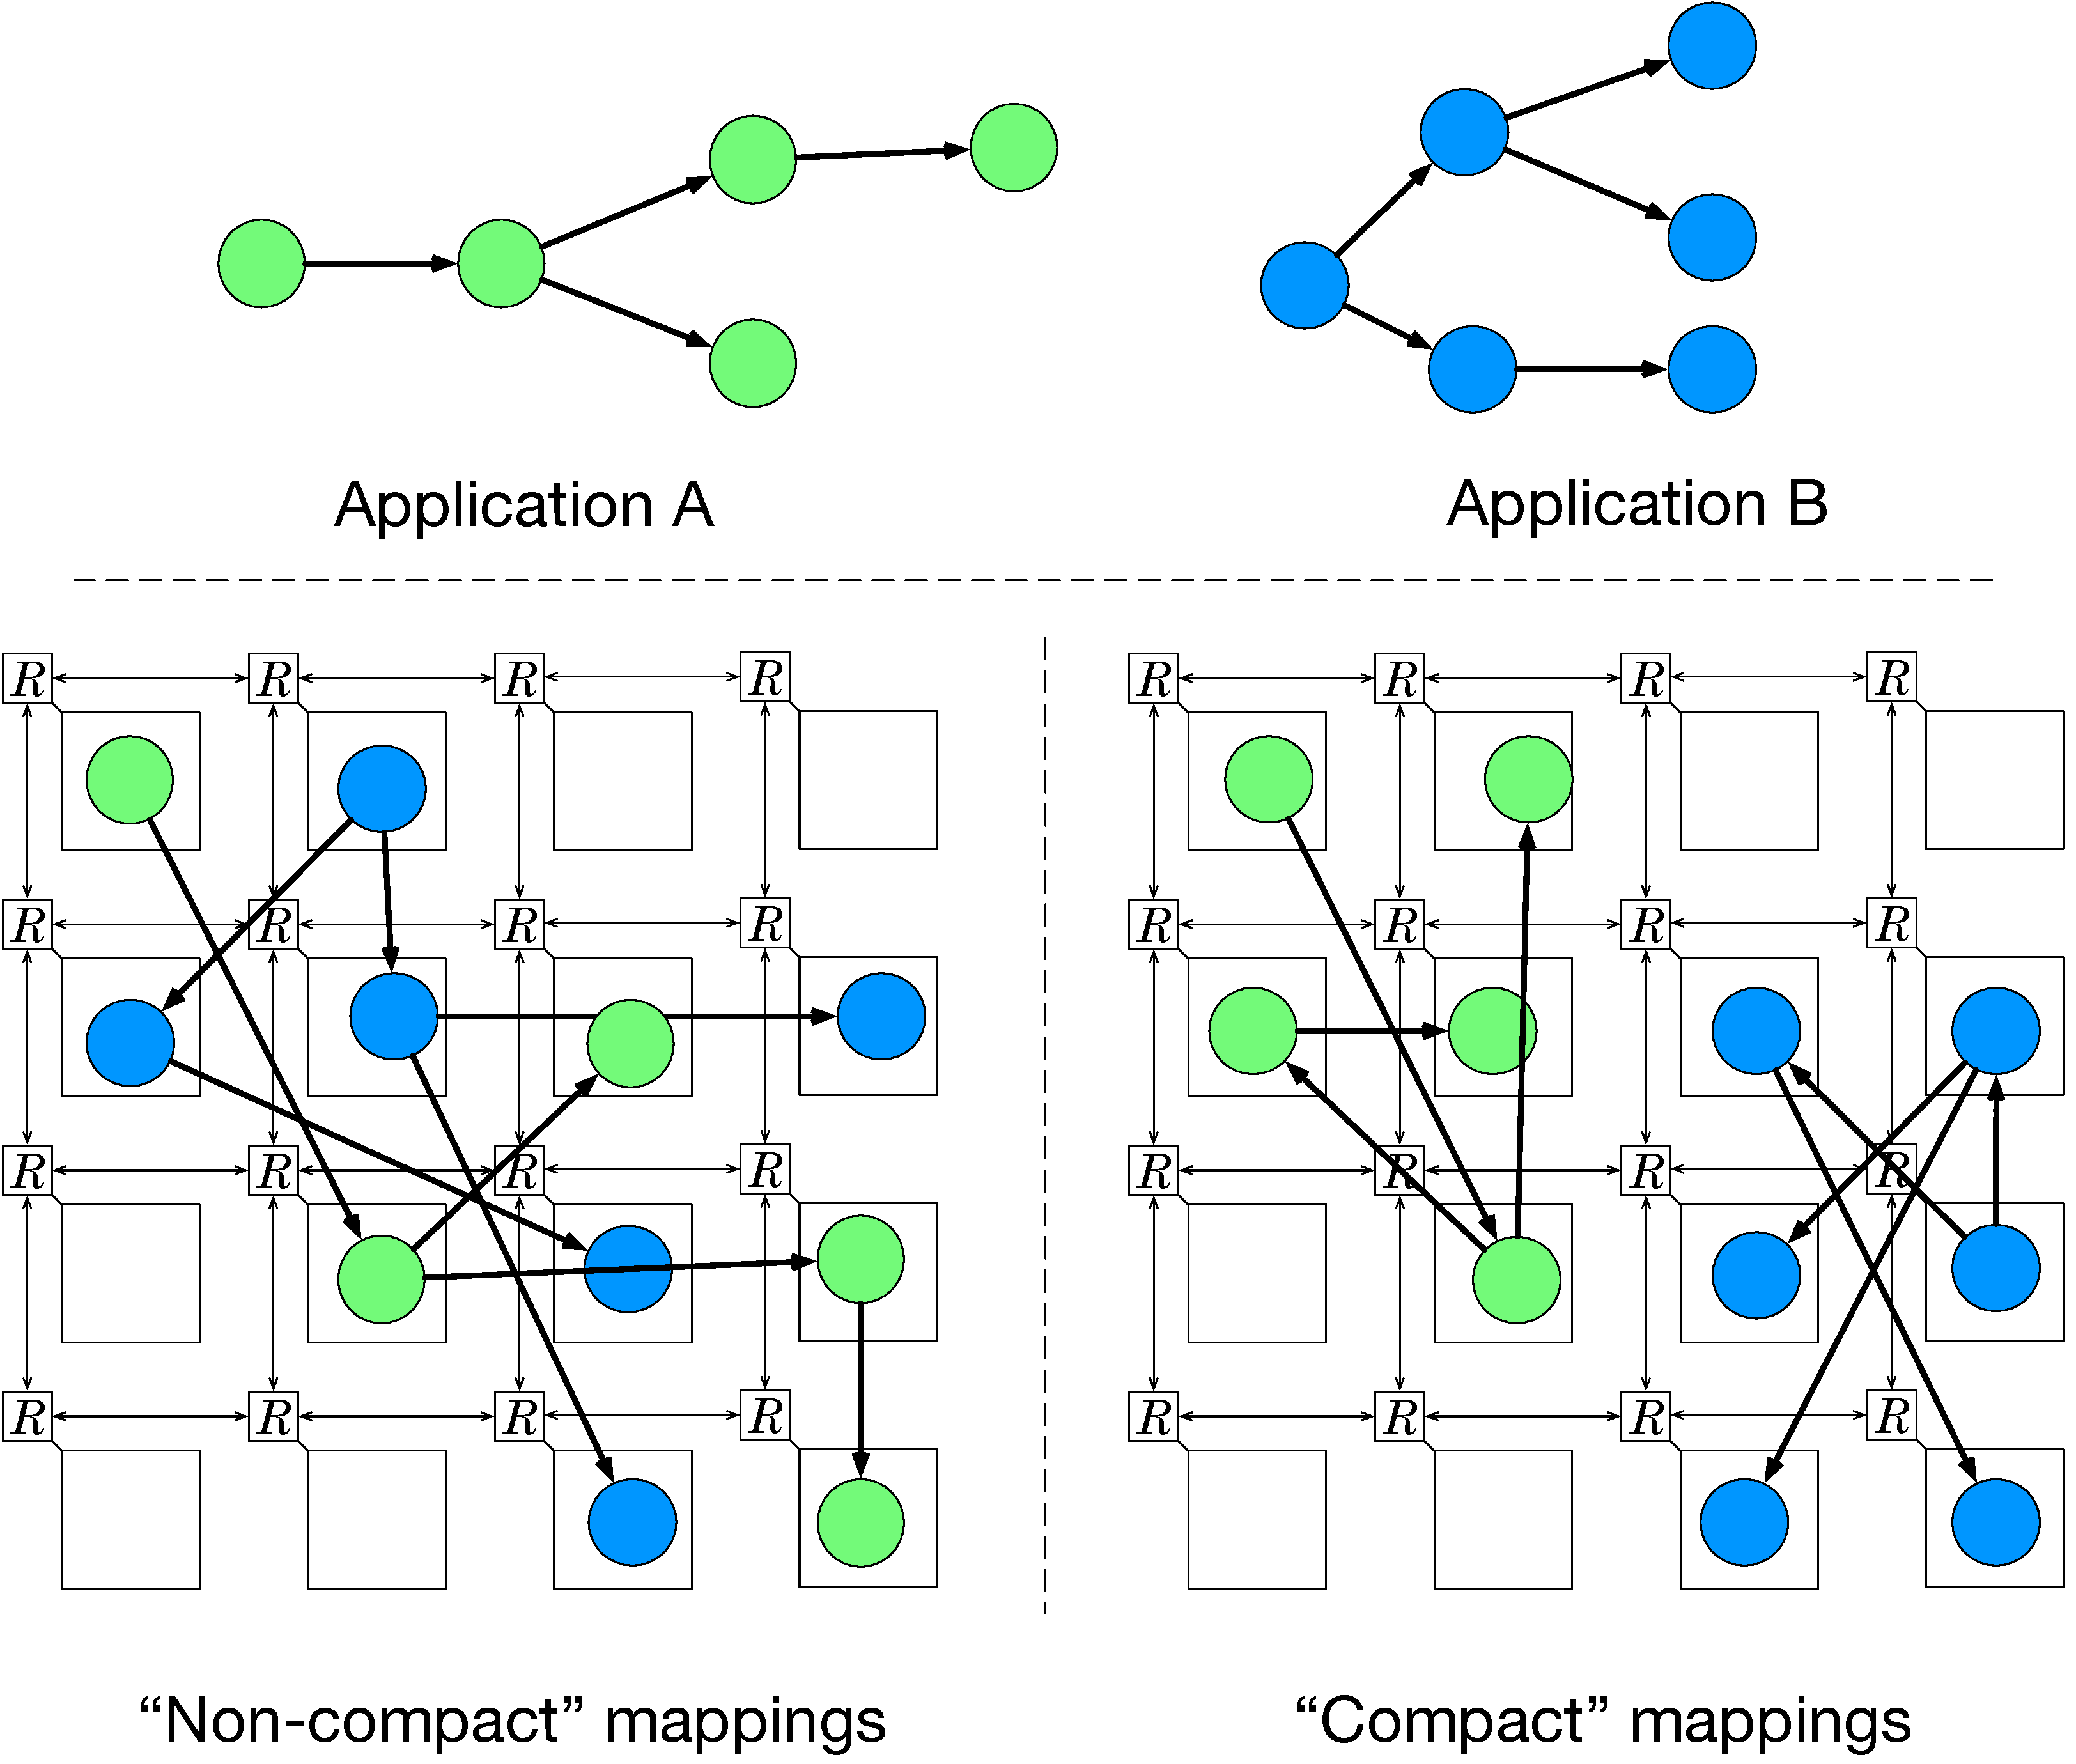
\includegraphics[width=0.6\textwidth]{figures/compact_intro.pdf}
	\caption{Equivalent mappings of two applications, one being compact and the other one not. Adapted from Figure~1 in~\cite{goens_samos19}.}
	\label{fig:compact_intro}
\end{figure*}

Figure~\ref{fig:compact_intro} illustrates well the idea of compact mappings.
It depicts two variants for mapping the two application graphs depicted in the figure.
The particular property of these two variants is that they are equivalent from the point of view of the distances:
For any two connected nodes in one of the application graphs, the node distance in terms of number of hops between both nodes is identical in both mapping variants.

Idea behind compact mappings, and why it does not work. Basically:\cite{goens_samos19}

\begin{figure*}[th]
	\centering
	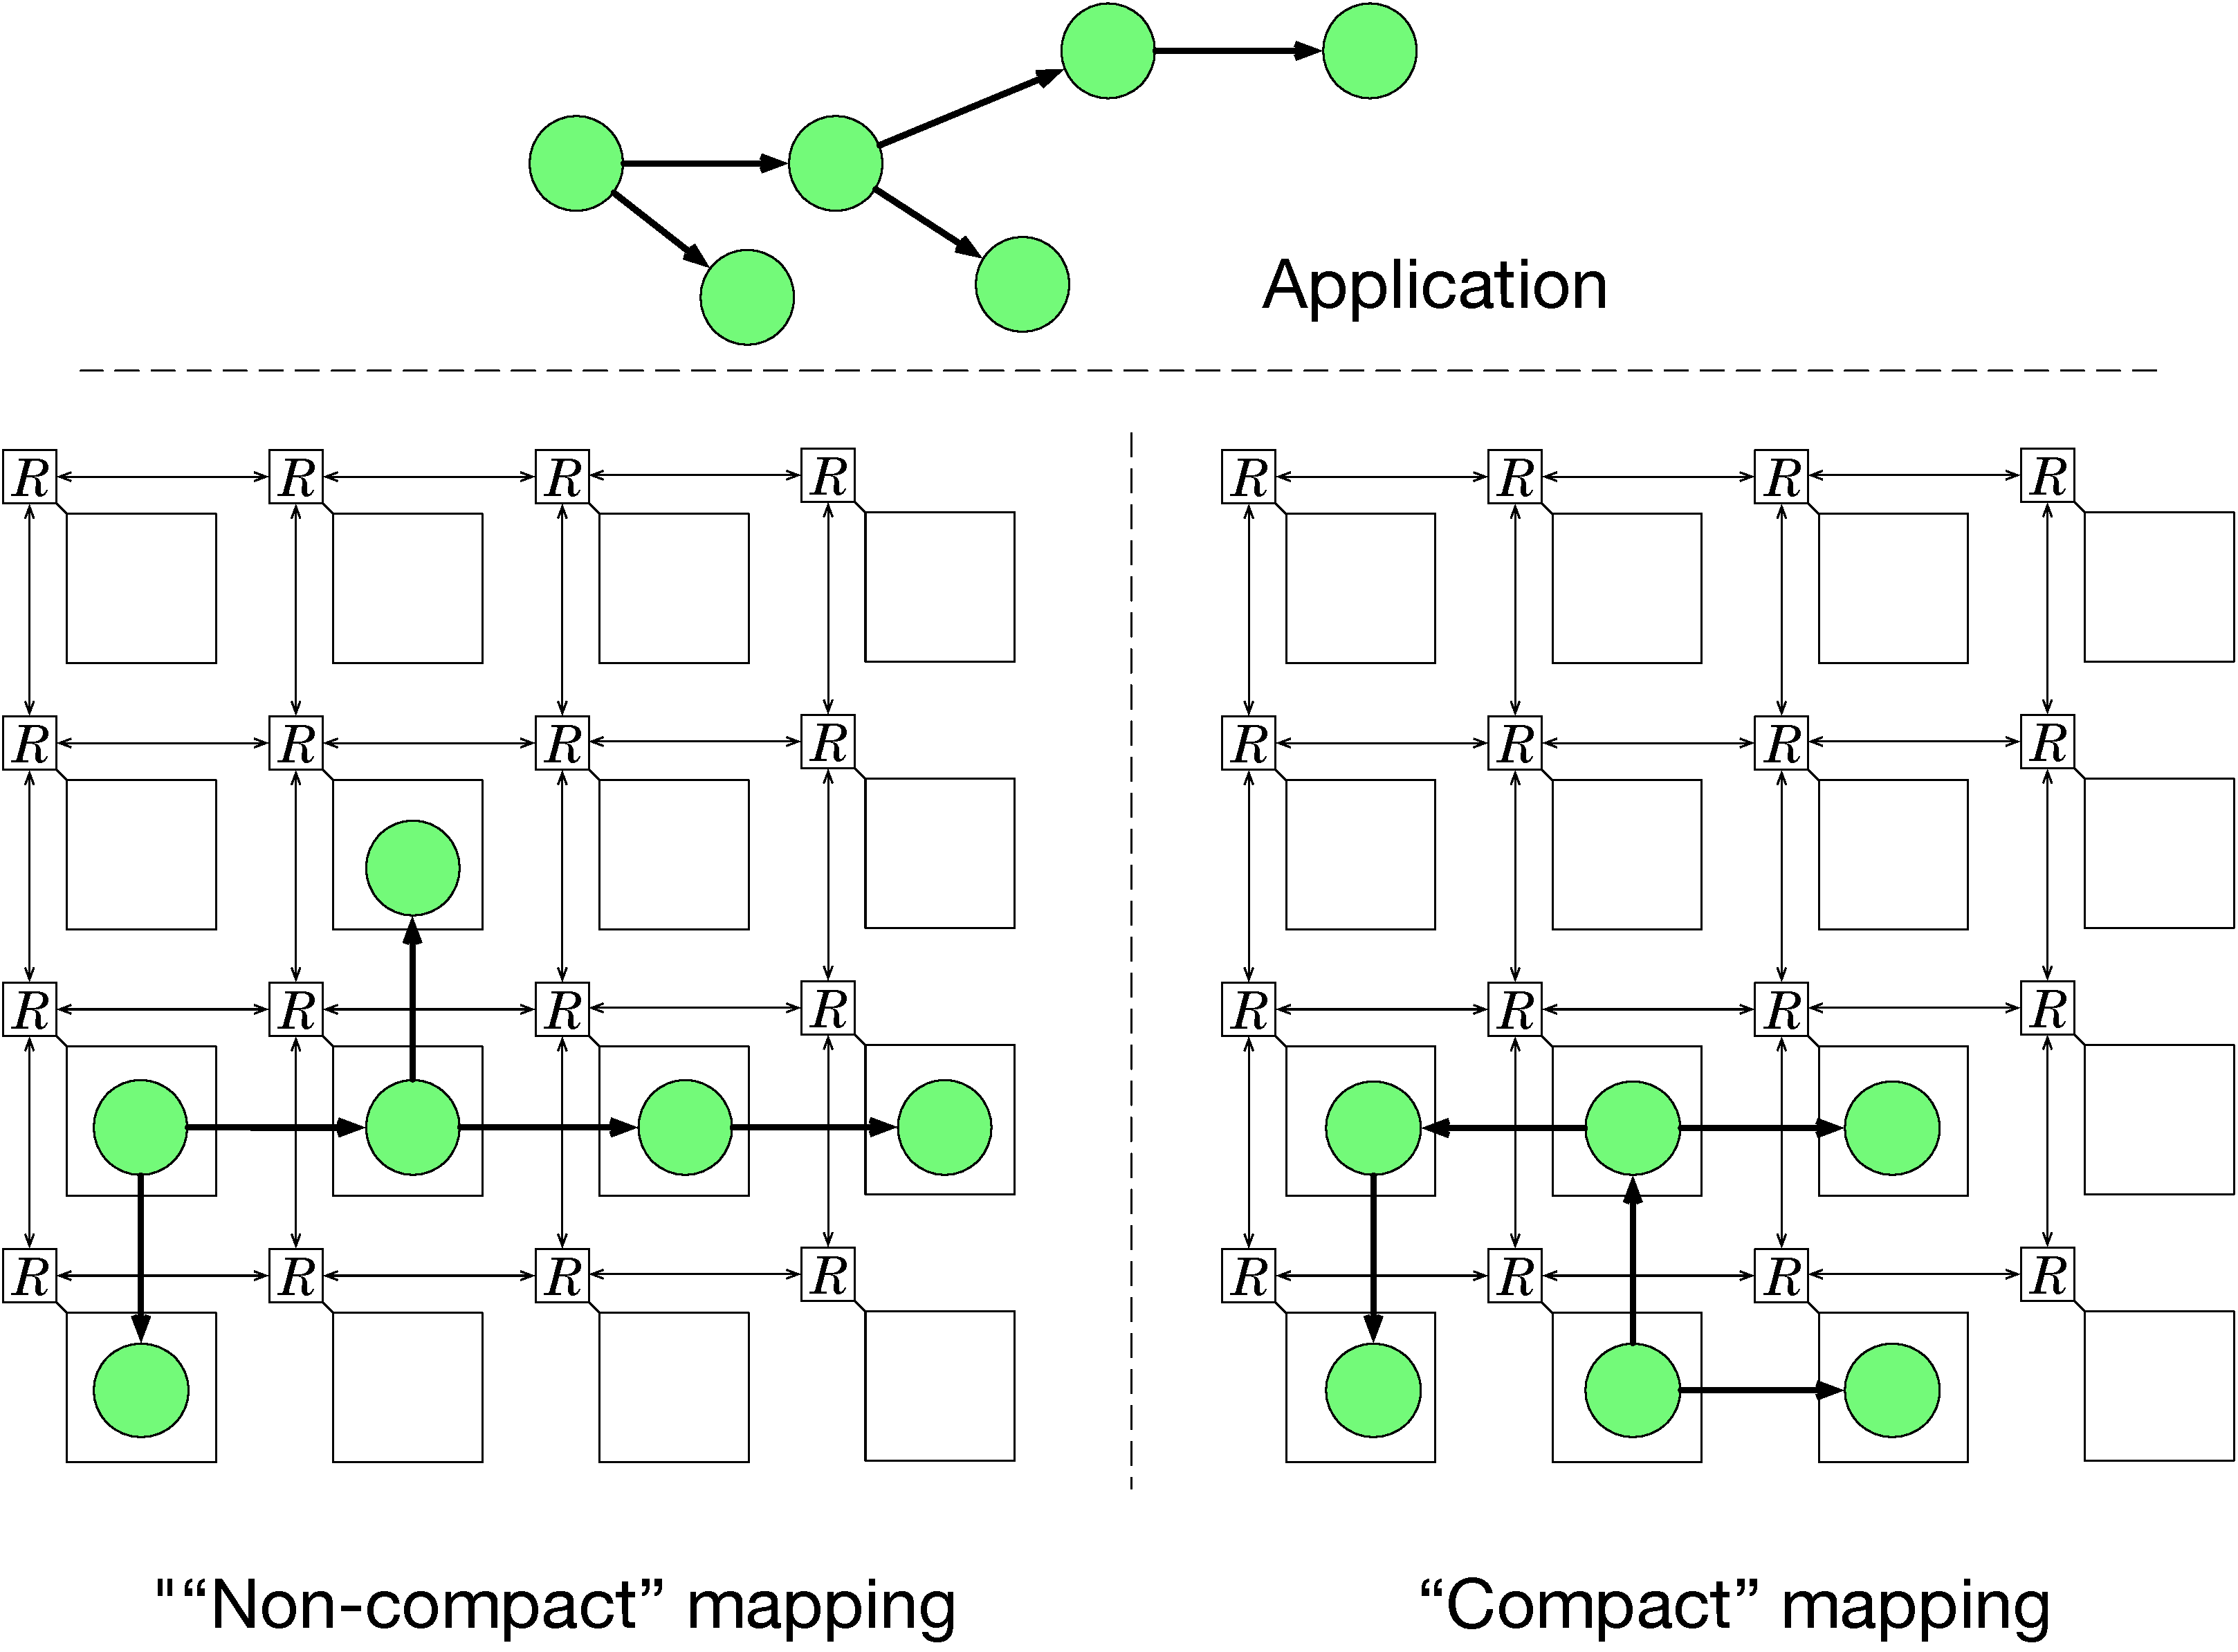
\includegraphics[width=0.6\textwidth]{figures/topology_vs_geometry.pdf}
	\caption{Two equivalent mappings that yield good performance. Adapted from Figure~2 in~\cite{goens_samos19}.}
	\label{fig:topology_vs_geometry}
\end{figure*}


\begin{figure}[h]
	\centering
   \resizebox{0.85\textwidth}{!}{\inputTikz{compact_latency.tex}}
	\caption{Comparison of latencies between compact, non-compact and random mappings. Adapted from Figure~4 in~\cite{goens_samos19}.}
	\label{fig:compact_latency}
\end{figure}


\begin{figure}[h]
	\centering
   \resizebox{0.85\textwidth}{!}{\inputTikz{compact_cases.tex}}
	\caption{Comparison between compact, non-compact and random mappings running isolation or with another 9 applications. Adapted from Figure~5 in~\cite{goens_samos19}.}
	\label{fig:compact_cases}
\end{figure} %samos19
\section{Robust Mappings}
\label{sec:design_centering}
Discuss first: \cite{hempel_scopes17}.

Then discuss using the new techniques.

Also open question: discrete vs continuous. %scopes17_dc + new
\section{Design Space Exploration}
\label{sec:dse}
As we saw in Chapter~\ref{chap:mapping}, a central step of model-based software synthesis is a \ac{DSE} step for finding mappings, among others.
We know the mapping space is intractably large and complex and we cannot find the actual optima in the space for any real-life problem sizes.
The best we can hope for are near-optimal mappings in a reasonable amount of time.
Thus, we focus both on the quality of the mappings as well as the time required.
This section will focus on \ac{DSE} for finding near-optimal mappings, as defined in Section~\ref{sec:mapping_problem}. 
We will see many applications of the structures defined and analyzed in Chapter~\ref{chap:mapping_structures}

\subsection{Heuristics and Metaheuristics}

Generally in \ac{DSE} we distinguish between two approaches for dealing with these kinds of intractable problems, heuristics and meta-heuristics (cf. Section~\ref{sec:mapping_problem}).
Recall that mapping heuristics are domain-specific algorithms that exploit the specific domain-knowledge to find a solution based on a pre-defined model of the problem, whereas meta-heuristics rely on an iterative evaluation of the points.
As we outlined above, different heuristics and meta-heuristics come with trade-offs between the exploration time required to find a solution and the quality of said solution.
This is certainly the case for many discrete optimization problems in general, the mapping problem being no exception~\cite{goens_mcsoc16}.
Commonly, meta-heuristics tend to find better results provided enough time, but require accordingly more time to do so.

A particular difficulty of comparing mapping approaches and algorithms are the different models used by different algorithms~\cite{goens_mcsoc16}.
With \mocasin we designed a common framework that allows us to compare between mapping algorithms~\cite{menard_rapido21}.
In particular, in \mocasin we have two heuristics for mapping: the \ac{GBM} heuristic~\cite{castrillon_dac12} and a static mapping variant~\cite{menard_rapido21} of the \ac{CFS} scheduler from Linux.
Additionally, we have implemented genetic algorithms based on and inspired by those found in Sesame~\cite{erbas2006multiobjective,quan2014towards,goens_mcsoc16}, a simulated annealing~\cite{simulated_annealing} mapping algorithm and a tabu search~\cite{tabu_search}.
We also have a simple random walk algorithm for reference.
A survey of these mapping algorithms, among others can be found in~\cite{singh2013mapping}.
We implemented these algorithms for \mocasin and this thesis to have a basis for comparison from established literature.

We first compare these mapping algorithms to establish a baseline. 
We execute a random walk $500$ random iterations.
For the genetic algorithm we run an evolutionary $\mu + \lambda$ strategy for $20$ generations of population size $10$, crossover rate of $1$ with probability $0.35$ and mutation probability $0.5$, with a tournament selection with tournament size $4$.
For the \ac{GBM} algorithm we set the parameters as \texttt{bx\_m} of $1$, \texttt{bx\_p} of $0.95$, \texttt{by\_m} of $0.5$,\texttt{by\_p} of $0.75$, 
The simulated annealing heuristic we execute with an initial temperature of $1$ and a final temperature of $0.1$, with a temperature proportionality constant of $0.5$  and a random movement starting radius of $5$.
Finally, for the tabu search mapper we set a maximum of $30$ iterations, each of size $5$ and with a move set size of $10$ and tabu tenure of $5$, and a random candidate move update radius of $2$.
These parameters were chosen such that the mappers seemed to yield good result, yet not systematically (e.g. using something like Bayesian optimization or general (hyper-)parameter optimization approaches).
A deliberate choice in the parameters however is that the exploration times should be comparable between the meta-heuristics, i.e. such that the iterative mappers evaluate a similar amount of mappings.

\begin{figure}[h]
	\centering
   \resizebox{0.95\textwidth}{!}{\input{generated/heuristics_vs_metaheuristics.tex}}
	\caption{Comparison of multiple mapping heuristics and metaheuristics on the \ac{E3S} benchmarks.}
	\label{fig:metric_comparison}
\end{figure}

Figure~\ref{fig:metric_comparison} shows a comparison of the different heuristics and metaheuristics on the \ac{E3S} benchmarks.
Each of the metaheuristics that require random data we execute $10$ times and show the variation as calculated by the unbiased estimator of the standard deviation of the multiple sampled times.
The execution times vary obviously depending on the different benchmark applications and on the platforms they run on.
The absolute values of these times, however, are not interesting for comparing the mapping algorithms.
We thus norm the values of the execution times, taking the results of the genetic algorithms as baseline.
We then aggregate all values with the geometric mean.
The error bars in the plot are calculated by taking the average value $\pm$ the estimated standard deviation and norming each of the two extremes, the results of which are the extremes shown in the plot.

We first examine the results for the Odroid XU4 architecture.
The two heuristics find considerably lower results in average, but they do so in considerably less time.
More concretely, they yield about an order of magnitude worse results in about an order of magnitude less time.
The results of the random walk heuristic are significantly worse than those of the more structured metaheuristics, even though it takes a comparable amount of time.
This is due to a deliberate choice, since as explained above, the number of random mappings was chosen specifically to be comparable to the number the number of mappings evaluated by the other meta-heuristics.
Since $500$ mappings is not a small amount, it is not terribly surprising that the random mapper beats the two heuristics.
Finally, the best mappings are found by the simulated annealing meta-heuristic, albeit only by $3\%$ compared to the genetic algorithm.

When we turn our attention to the significantly larger and more complex MPPA3 Coolidge architecture, we see that the picture changes drastically.
The marked difference between heuristics and meta-heuristics disappears in this case.
The \ac{GBM} heuristic is on par with the random walk results in average, while taking substantially less time.
This is simply explained by the significantly larger design space of mapping to the MPPA3 Coolidge.
In this case, the genetic algorithm significantly outperforms both other meta-heuristics, by a factor of $4-5$, while taking less time.
The most striking result here, however, is the extremely good performance of the static CFS heuristic.
This good performance is misleading at first, a perhaps more honest assessment of the results is that \emph{all other (meta-) heuristics perform poorly}.
We can interpret this as a consequence of the growing design space and its complexity, which affects the metaheuristics, while the static CFS mapper can still leverage domain-specific knowledge to find fairly good mappings.

TODO: add and test genetic with CFS initials.

\subsection{Leveraging Symmetries}
Talk about~\cite{goens_taco17} + new stuff (mpsym)

\subsection{Leveraging Metric Spaces}
Improving DSE algorithms with metric spaces?

Talk about gradient descent: why it does not work w/o metric space structure, and why it should with it.
\begin{figure}[h]
	\centering
   \resizebox{0.95\textwidth}{!}{\input{generated/geometric_heuristics_coolidge.tex}}
	\caption{The effect of embedding-based representations in metaheuristics that leverage the geometry on the MPPA3 Coolidge platform.}
	\label{fig:coolidge_geometric}
\end{figure}

We can take two observations from these results and combine them.
The first one is the knowledge that geometry-based heuristics indeed benefit from a better metric, independent of if the resulting heuristics are overall good.
The second observation is more subtle, it's about the general structure of the design space. 
An observation we can make is that 

\begin{figure*}[t]
  \centering
	\begin{subfigure}[b]{0.43\textwidth}
    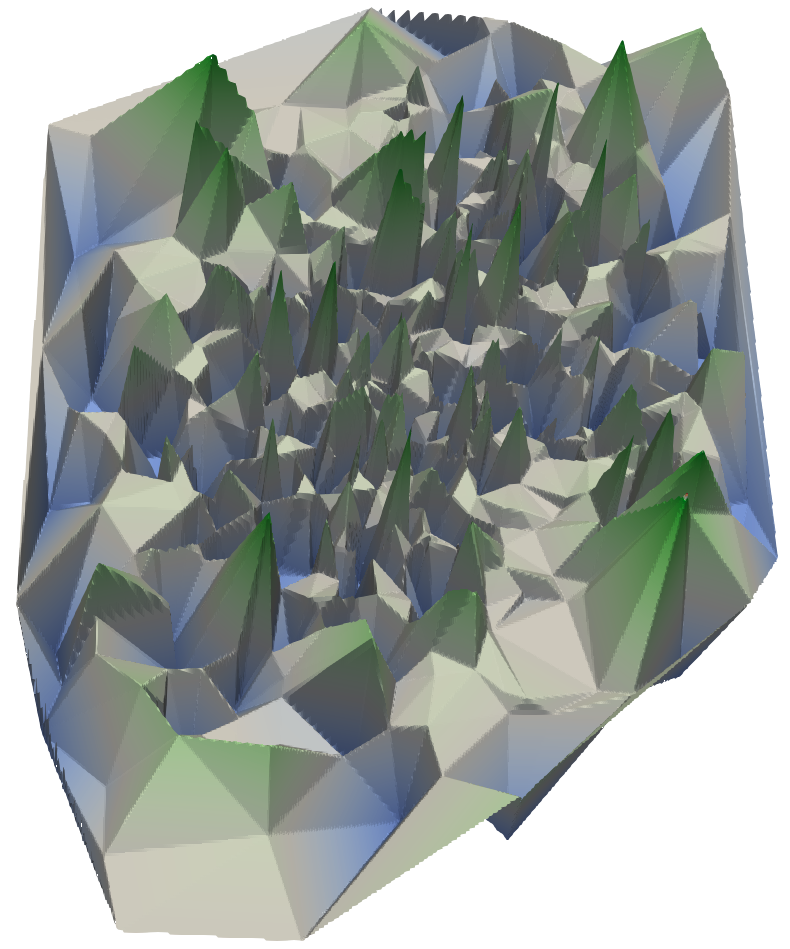
\includegraphics[width=\textwidth]{figures/coolidge-af-space-sim-vec.png}
		\caption{SimpleVector}
		\label{fig:lvars-bench-cores}
	\end{subfigure}
	~
	\begin{subfigure}[b]{0.43\textwidth}
    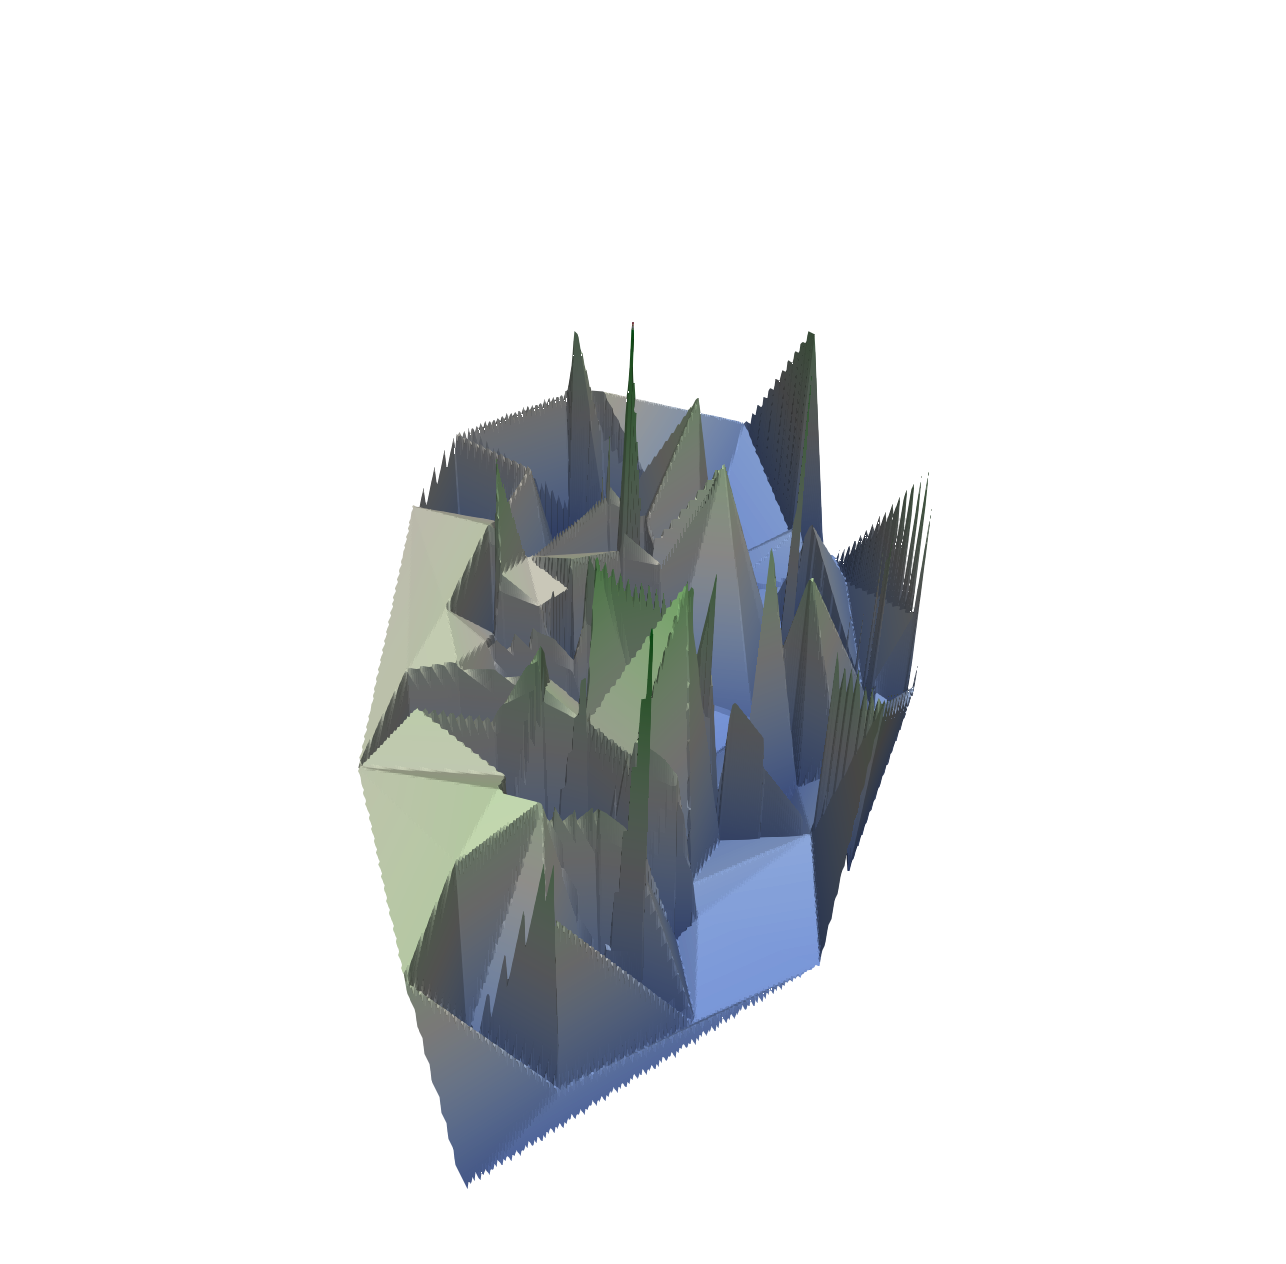
\includegraphics[width=\textwidth]{figures/coolidge-af-space-emb-sym.png}
		\caption{SymmetryEmbedding}
		\label{fig:lvars-bench-overhead}
	\end{subfigure}

	\caption{Visualization of the same design space of the audio filter benchmark on the MPPA3 Coolidge platform in two different representations.}%
	\label{fig:visualization_simpvec_symemb}
\end{figure*}

\subsection{All Representations}
\begin{figure}[h]
	\centering
   \resizebox{0.95\textwidth}{!}{\input{generated/multiple_representations_exynos.tex}}
	\caption{Comparison of the effects of multiple representations on the Odroid XU4 platform.}
	\label{fig:multiple_representations_exynos}
\end{figure}

\begin{figure}[h]
	\centering
   \resizebox{0.95\textwidth}{!}{\input{generated/multiple_representations_coolidge.tex}}
	\caption{Comparison of the effects of multiple representations on the MPPA3 Coolidge platform.}
	\label{fig:multiple_representations_exynos}
\end{figure} %taco, mcsoc18
%Here should go an intro to this chapter.

\section{A Language for Describing Mappings}
\label{sec:logic_language}
The \acf{IoT} is a term used to describe the phenomenon that many modern embedded devices have internet connectivity and can all be interconnected this way.
This opens many opportunities for automation and increased interconnectivity. 
Sensors and actuators in \ac{IoT} devices can be combined to add new functionalities to the system that would not be possible for the individual devices.
In~\cite{weber_phdthesis} a case is made for \emph{spatial ontologies} through a logical language they call \emph{semantic localization}, to reason about distances in the real world in multiple representations, as found in the different \ac{IoT} devices.\index{ontologies}
These different representations of distances are not unlike the different representations of mappings discussed in Section~\ref{sec:representations}.
In analogy to semantic localization, in this section we describe how we can define a locgical language that permits querying and combine representations of mappings, or \emph{mapping ontologies}\footnote{Ontologies have a well-defined meaning in logic and theoretical computer science, which we allude to, but not precisely mean here. We use the word here in its more everyday (philosophical) sense of meaning its existence or reality.}, in a uniform fashion.
This language is based on first-order logic and also includes implicit domains and relations to define and combine statements in the different ontological representations of mappings.

Depending on the context, different representations of the mapping space might offer extremely efficient ways of answering a particular type of question about a mapping.
In the \texttt{SimpleVector} representation, the question ``Is Task$_A$ mapped to PE$_3$'' is very easy to answer, whereas answering the question ``is the expected latency between Task$_B$ and Task$_C$ below $10 \mu s$?'' is more difficult to answer.
Conversely, in the representation based on the metric space topology,\texttt{MetricSpaceEmbedding}, with a metric defined by the communication distances between hardware resources, the difficulty of these two last questions might be reversed.
In order to efficiently find mappings thus, depending on the objectives, an algorithm might want to use a representation or the other, or perhaps a combination of them.

There is a distinct advantage in defining a language, as opposed to simply defining a series of programming interfaces to the different representations, and letting algorithm programmers combine them in a programmatic way using a general-purpose language, like Python.
By defining a domain-specific query language, we are creating a new level of abstraction that will hopefully allow researchers to reason about the mapping problem in new ways, transcending the simple usages to combine queries that will be presented in this section.

We describe go over the representations as defined in Section~\ref{sec:representations}, focusing on the kinds of questions they are well-suited to answer.
We then proceed to give examples of questions that might be asked, and how these could be combined using the language.
A language was implemented by Felix Teweleitt~\cite{teweleitt_studienarbeit} for \mocasin based on these principles.
We omit the details of the actual syntax and implementation of the language, as it falls outside the contribution of this thesis.

The \texttt{SimpleVector} representation is, as described throughout the previous chapters, the typical mapping representation that uses vectors of the form $ m = (p_1,\ldots,p_k,c_1,\ldots,c_l)$ to define the mapping.
It is well-suited to answer questions of the form:
\begin{itemize}
  \item Is task $A$ mapped to $PE_1$?
  \item Does $PE_2$ execute any process?
 \item Do tasks $A$ and $B$ execute on the same \ac{PE}?
\end{itemize}

The \texttt{Symmetries} representation representation normalizes mappings that are equivalent to a single (canonical) mapping, while still using the vector form (cf. Section~\ref{sec:symmetries}).
Some examples of well-suited questions for it are:

\begin{itemize}
\item Is this mapping equivalent to mapping $m'$?
\item Do tasks $A$ and $B$ execute on the same \ac{PE}?
\end{itemize}

The \texttt{MetricSpaceEmbedding} representation uses the communication topology to define meaningful distances between \acp{PE} and by extension, between mappings (cf. Section~\ref{sec:metric}).
This representation is well-suited to answer questions like:
\begin{itemize}
\item Is this mapping very similar to mapping $m'$? (can give false positives, as seen in Section~\ref{sec:metric})
\item Is the expected latency between tasks $A$ and $B$ under $10 \mu s$?
\end{itemize}

The \texttt{SymmetryEmbedding} representation combines the \texttt{Symmetries} and \texttt{MetricSpaceEmbedding} representations. As such, it combines the both their strengths and weaknesses as a mapping ontology.
Other representations, not necessarily based on metric spaces, could readily be added to this language. 
For example, we could design a hierarchy or inclusion-based distance with a way to define a \ac{PE} hierarchy with refinements (PEs $\in$ clusters $\in$ chips) and similarly for hierarchical applications.

\subsubsection{The Language}

The statements in the language refer to a mapping, i.e. every mapping in the mapping space either satisfies such a statement or it does not.
Thus, the questions motivated for the different representations above can be combined in a single statement, like:
``Is this mapping very similar to $m'$ (distance $\leq 100$) \emph{and} \emph{not} Is this mapping equivalent to $m'$ \emph{and} (\emph{there exists} a PE $p$ such that tasks $A, B$ and $C$ are mapped to $p$ \emph{or} (the expected latency between tasks $A$ and $B$ is small than $10$ \emph{and} the expected latency between tasks $B$ and $C$ is smaller than $10$ \emph{and} the expected latency between tasks $A$ and $C$ is smaller than $15 \mu s$)).''

In this language, a special solver tries to find a solution to a statement (i.e. a mapping) or a set of such solutions by evaluating the propositions in the statement in a specific order.
For example, if we have a propositional statement in conjunctive normal form, we can solve the different conjuncts iteratively.
Since a mapping has to satisfy each of them, the final mapping can be found by first filtering a large portion of mappings with the strongest conjunct, and iterating from there.
In his work, Felix Teweleitt designed a solver for \mocasin which utilizes a simple heuristic with precisely this principle to solve some queries~\cite{teweleitt_studienarbeit}, but there is potential for much more sophisticated solving methods.

We choose to extend propositions about mappings to first-order logic so that we can have quantifiers only valid for some specific domains, like mappings, \acp{PE}, hardware communication resources, tasks (or processes or actors), communication channels.
It is clear why and how these domains are the ones we can quantify over for first-order formulas describing mappings.
An additional idea would be to include physical distances (over a discrete set of distances).
This can be combined with different spatial ontologies in semantic localization for the \acf{IoT}~\cite{weber_phdthesis}. 
This way, we could define \ac{IoT}-mappings that have specific requirements specified in our logical mapping  language.

A vision of such \ac{IoT} mappings could be the following example:
A smart autonomous car enters a smart parking lot.
The parking lot is dark and pretty full already, and the car is low on battery, so that it needs to find a parking space with a suitable recharge station.
To navigate in this dark environment, the smart car needs to offload its pedestrian recognition algorithm to a service in the parking lot, which it does by using an ontology-powered service discovery~\cite{weber2019service} mechanism.
Since the large concrete structure of the mapping space blocks the signal, only some very close-by servers in the smart parking lot are suitable for offloading computation with low latency and high reliability.
Spatial ontologies have to be included in the mapping query to offload the high-performance pedestrian recognition in a dark environment.
Furthermore, for legal reasons, the car cannot offload some decision-critical parts of the computation to an external device.
This complex set of constraints on the \ac{IoT} mapping can be formulated in a mixed-ontology sentence, which includes a successor of our logical mapping language with multiple representations, as well as other \ac{IoT}-ontologies like semantic localization.

Clearly this vision is very far removed from today's reality, but it explains the motivation for a logical language and mapping ontologies based on the representations as discussed in this thesis. %taco, mcsoc18
\section{Run-time applications: TETRiS}
\label{sec:tetris}
So far, the applications of the structures we have discussed are primarily useful at compile- or design-time.
In this section we will discuss \acs{TETRiS}, a hybrid mapping approach where the structure of mapping symmetries are useful at run-time.

In Section~\ref{sec:symmetries} we saw how the symmetries of the mapping problem define multiple mappings to be equivalent.
We expect mappings that are equivalent to have the same runtime or energy consumption. Indeed, the simulation results are identical for equivalent mappings.
When leveraging this structure for \ac{DSE}, we consider only one of the multiple equivalent mappings, disregarding the rest, since they yield identical results in a simulation.
The \acf{TETRiS} approach~\cite{goens_scopes17} leverages this property in a complementary fashion, by selecting equivalent variants at run-time according to the current system load.
While this works for a single mapping, the strength of \ac{TETRiS} lies in selecting from different mappings with different properties first and using the equivalent variants to find a multi-application schedule.

\begin{figure*}[th]
	\centering
	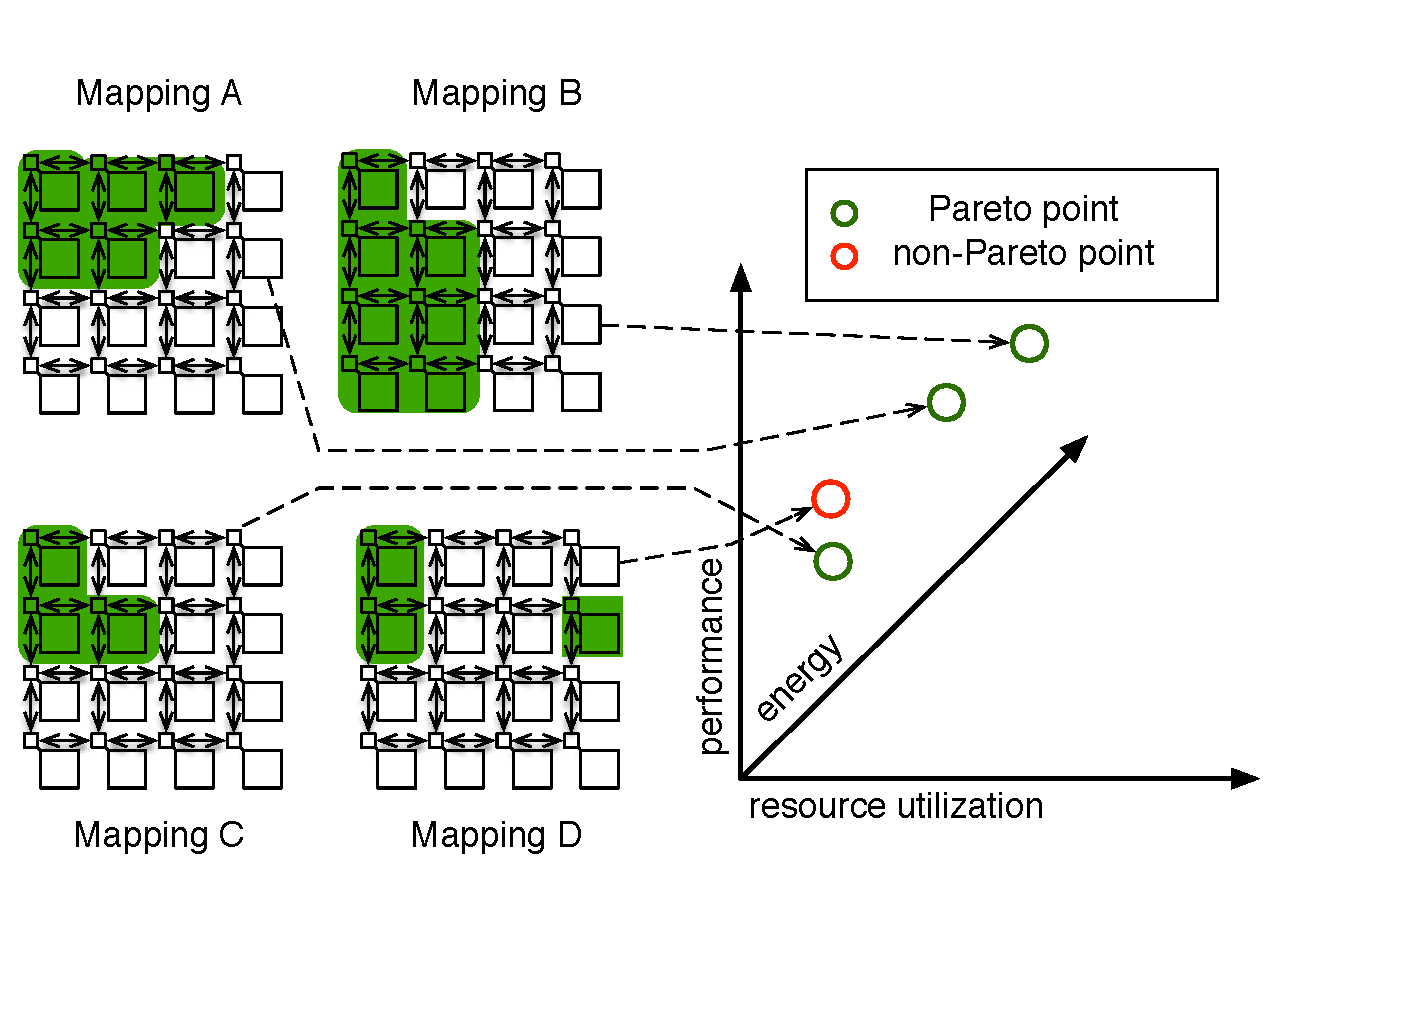
\includegraphics[width=0.7\textwidth]{figures/pareto_mappings.pdf}
	\caption{An illustration of Pareto points in the mapping space.}
	\label{fig:tetris_pareto}
\end{figure*}

We say that a design point (mapping) $m_1$ \emph{dominates} another $m_2$ if for the objective property $\Theta$, $m_1$ is at least as good as $m_2$: $\Theta(m_1) \leq \Theta(m_2)$. \index{dominated}
Recall that as defined in Equation~\ref{eqn:mapping_min_problem}, $\Theta$ is a multi-objective function and the comparison $\Theta(m_1) \leq \Theta(m_2)$ is to be understood component-wise, i.e. for each objective $i$, $\Theta_i(m_1) \leq \Theta_i(m_2)$.
A Pareto point is a design point (mapping), which is not dominated by any other design points. 
The different mappings \ac{TETRiS} chooses from are, ideally, Pareto points in the space of properties we are interested in.\index{Pareto point}
Figure~\ref{fig:tetris_pareto} illustrates this for the properties of energy, performance and resource utilization.
Each of the green points in the property space depicted to the right of the figure is a Pareto point.
It is better than every other point in at least one of the properties (performance, energy or resource utilization).
Only the red point corresponding to Mapping D is dominated by Mapping C, which utilizes the same number of resources, while being faster and more energy efficient.

The selection algorithms based on the desired properties are beyond the scope of this thesis, but \mocasin has implementations of multiple such algorithms~\cite{khasanov_date20}.
Once a mapping has been selected for each application, they need to be combined in a multi-application mapping.
This is where the symmetries come into play. 

\begin{figure*}[th]
	\centering
	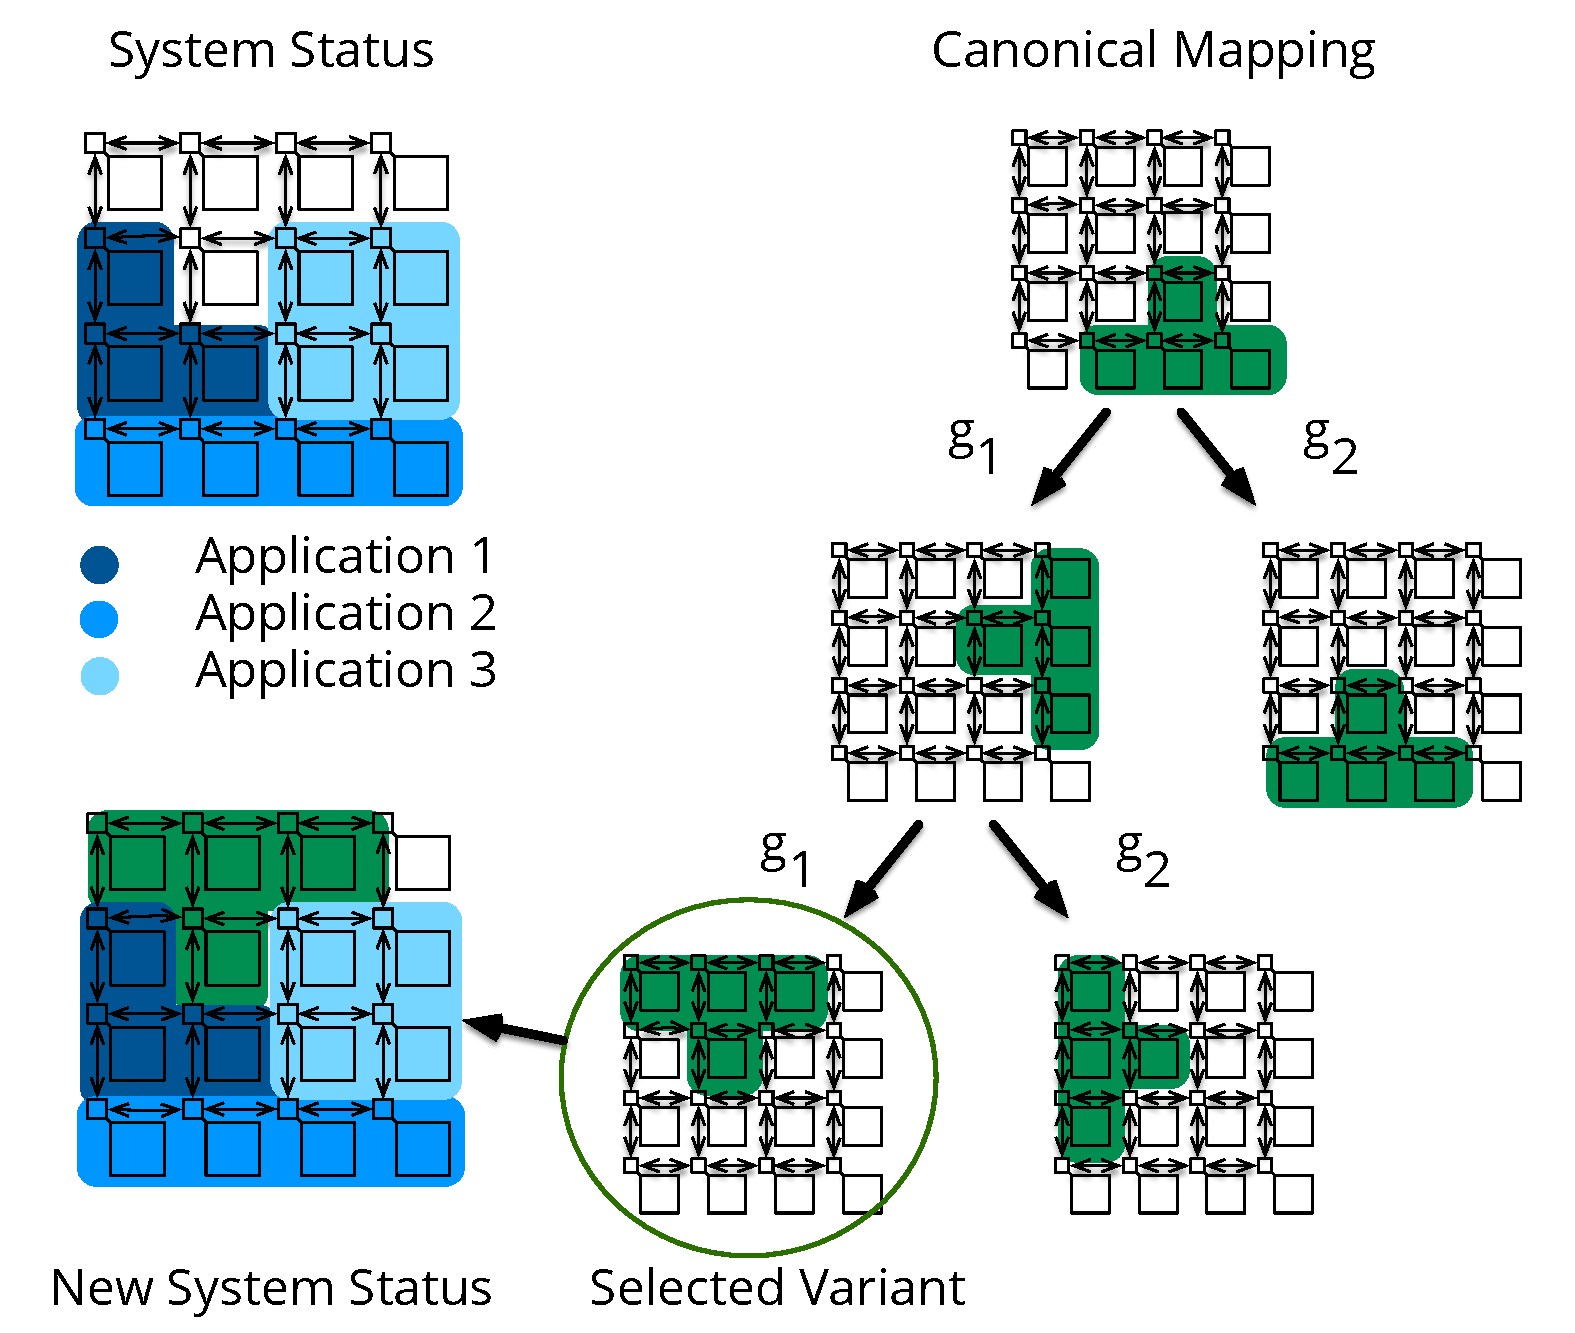
\includegraphics[width=0.8\textwidth]{figures/Variant_Selection.pdf}
	\caption{Variant selection in \ac{TETRiS}.}
	\label{fig:tetris_variant_selection}
\end{figure*}

Figure~\ref{fig:tetris_variant_selection} depicts the principle behind this symmetry-enabled variant selection.
At this point we assume a mapping has been selected, which we call the \emph{canonical mapping} in reference to the canonical representative of the equivalence class (orbit).\index{\ac{TETRiS} ! canonical mapping}
\ac{TETRiS} keeps track of the system's status, knowing where other running applications are mapped.
The idea behind the variant selection is then to apply the generators $g_i \in G$ of the automorphism group $G$ for the mapping space. 
We call the process of applying these generators \emph{\ac{TETRiS} rotations}, informed by the geometric intuition of these transformations\index{\ac{TETRiS} ! rotations}\footnote{This might be reminiscent of the commercial game Tetris (Тетрис). Note that the \ac{TETRiS} system is an independent research project and any resemblance is purely coincidental.}

\begin{figure*}[th]
	\centering
	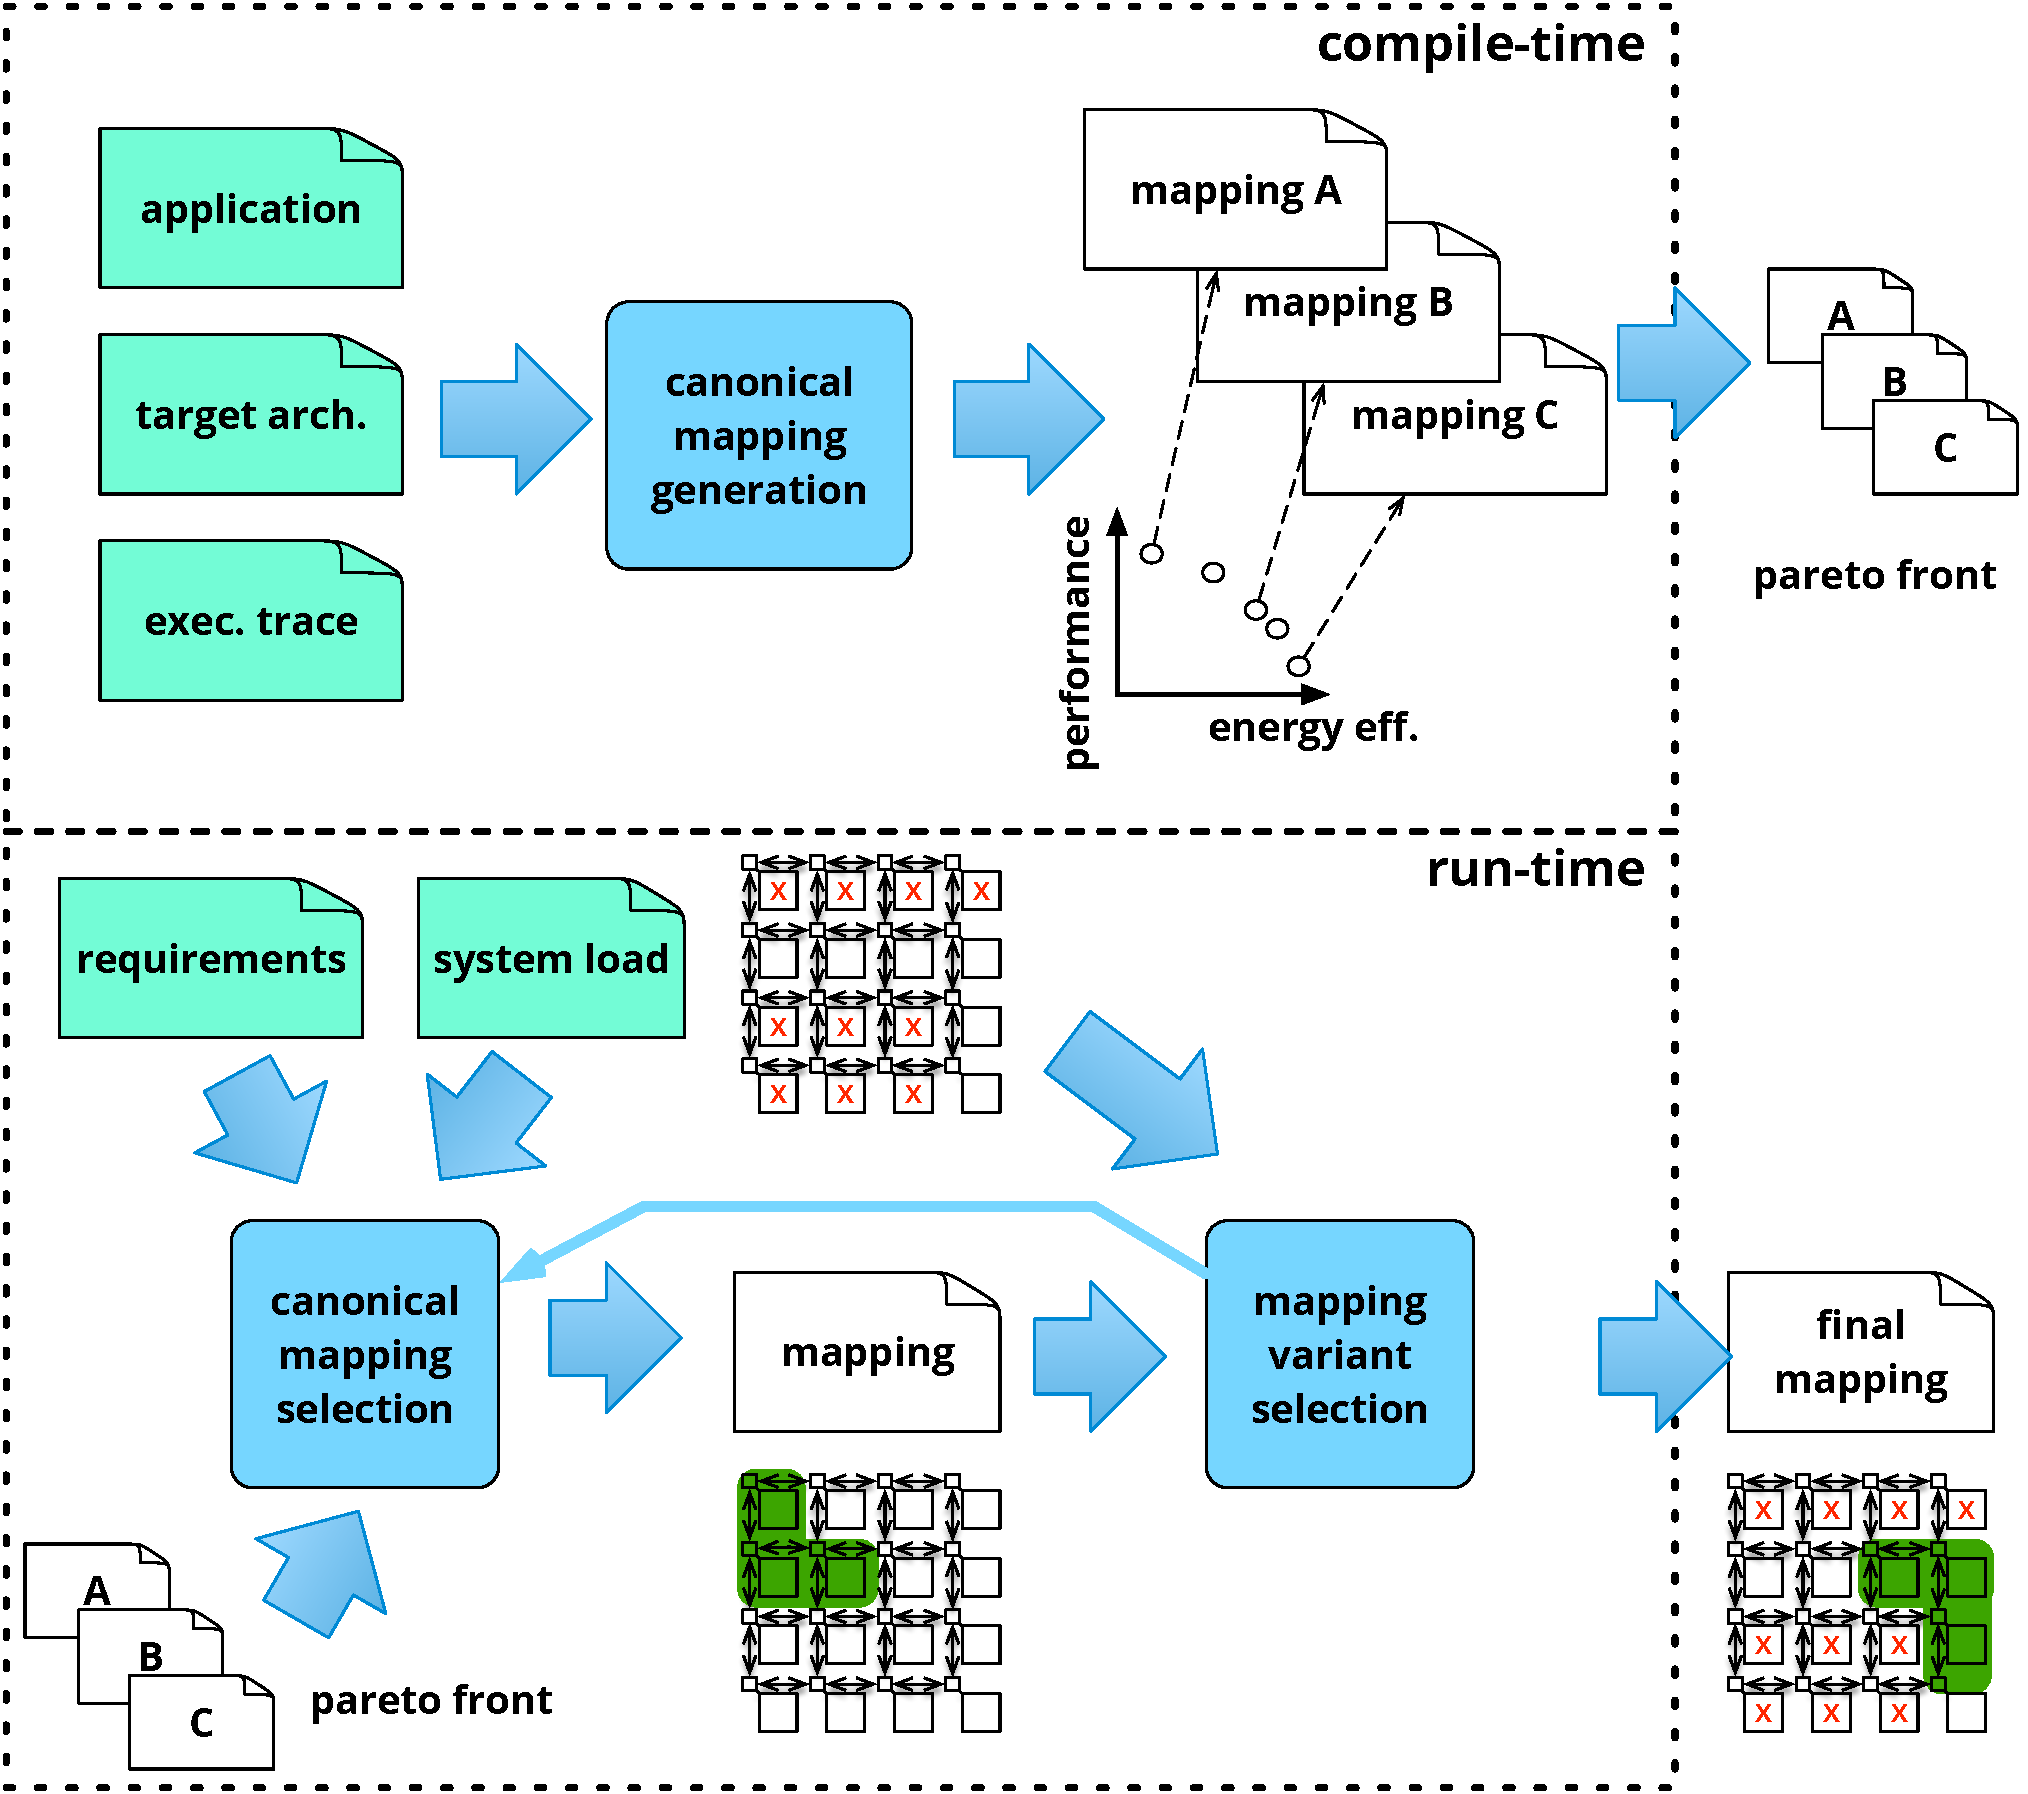
\includegraphics[width=1.00\textwidth]{figures/tetris_flow.pdf}
	\caption{The \ac{TETRiS} flow.}
	\label{fig:tetris_flow}
\end{figure*}

Combining the principles outlined above, Figure~\ref{fig:tetris_flow} shows the general flow of the hybrid \ac{TETRiS} approach. 
In a compile-time phase, so-called \ac{TETRiS} canonical mappings are generated as Pareto points in a multi-objective design space which ideally includes the system's resources as an objective.
Then, at run-time, a selection algorithm decides which canonical mapping to use based on the requirements (e.g. real-time constraints) and possibly also based on the system's load.
The selected canonical mapping is then placed onto the system by leveraging the symmetries of the mapping space in a variant selection phase, generating a final run-time mapping.
When generating mappings with this method, we can guarantee the spatial isolation of computation.
Provided the contention in communication is not too large, this also means that the properties of the canonical mappings are preserved (cf. Section~\ref{sec:compact}).
We tested this on an Odroid XU4 system running a pthread-based implementation\footnote{\url{https://github.com/l3nkz/tetris}} of the \ac{TETRiS} principle~\cite{goens_scopes17}.

\begin{figure*}[th]
	\centering
   \resizebox{0.95\textwidth}{!}{\inputTikz{tetris_experiment.tex}}
	\caption{Comparison of the TETRiS system with Linux' \acs*{CFS} executing four instances of the audio filter benchmark simultaneously an Odroid XU4. Adapted from Figure~9 in~\cite{goens_scopes17}.}
	\label{fig:tetris_experiment}
\end{figure*}

Figure~\ref{fig:tetris_experiment} shows the results of this test.
It compares the Linux \ac{CFS} with our \ac{TETRiS} system when running for instances of the audio filter benchmark (\ac{CPN}).
The three mappings $T_1$, $T_2$ and $T_3$ are three different Pareto points in terms of wall-clock time, CPU time and energy consumption. 
The mapping \ac{CFS} refers to an execution using Linux' \ac{CFS} scheduler and thus technically without a (static) mapping, which we measured for comparison.
For each mapping we executed the four concurrent instances of the application and measured the wall-clock and execution times as well as the total energy consumption.
We see that the execution of applications with \ac{TETRiS} is indeed significantly more predictable than with the dynamic approach of \ac{CFS}.
This is especially clear for the execution times, where the variance of \ac{CFS} of around $1.3 \cdot 10^{-1} s$ is two orders of magnitude higher than that of \ac{TETRiS}, which for example for $T_3$ is only  $2.7 \cdot 10^{-3}s$.
However, the difference is also very clearly visible for the energy consumption. The variance of \ac{CFS} is around $2.9 J$, whereas that of \ac{TETRiS} for $T_3$ is around $6.9 \cdot 10^{-1} J$, about an order of magnitude lower. %scopes17_tetris + new
\section{Memory Allocation}
\label{sec:memory}
Discuss how memory is usually not considered.

Veery briefly summarize~\cite{odendahl_date14,goens_jsa16,odendahl15}.

Segway into emerging memory technologies: example \ac{RTM}. Discuss~\cite{khan_date20}, mostly discuss connections to DSE (genetic) and ILP formulations (my contribution). Be careful to delineate contributions here.
 %date14,jsa16,date20_rt

%\chapter{Conclusions}
%Here will be a part I conclusion.

%
%\chapter{Related Work}
%The nature of this thesis is not focused enough for us to discuss related work from a general point of view.
Perhaps the closest in spirit to the work presented in this thesis is the Ptolemy project~\cite{Ptolemaeus:14:SystemDesign}.
It is a tool for exploring model-based design and has a strong focus on \acp{cps}.
The Ptolemy project is very comprehensive and studies and implements several \acp{MoC} discussed in this thesis (cf. Section~\ref{sec:mocs_overview}).
The scope of the Ptolemy project is far larger and more detailed than this thesis.
It is, however, aimed at application developers.
In contrast, the methods in this thesis are aimed at tool developers, for improving the methods of model-based design.

Instead of discussing related work generally, we will go over on the different methods proposed here to improve model-based design, and discuss related work by broader categories.
In most chapters and sections we discuss related work directly.
While we will systematically go over related work here, we will refer to the according sections for discussion.

\paragraph{Dataflow-based Software Synthesis}
We used and discussed the \ac{MAPS} framework~\cite{maps} and its spinoff in Silexica, as well as the \mocasin tool where we implemented many contributions of this thesis.
These tools are both closely related, \ac{MAPS} focusing more on application developers and \mocasin on tool developers (for developing tools like \ac{MAPS}).
There are many closely related tools, like Sesame~\cite{pimentel2006systematic}, DOL~\cite{thiele2007DOL}, SystemCoDesigner~\cite{haubelt2008systemcodesigner}, DAARM~\cite{weichslgartner2014daarm}, PREESM~\cite{pelcat2014preesm}, Spider~\cite{heulot2014spider}, CAPH~\cite{serot2013caph} and Turnus~\cite{casale2013turnus}, among others.
Section~\ref{sec:software_synthesis_flows} discusses these tools more in-depth.

\paragraph{Other software synthesis tools}
The tools above focus on software synthesis in a flow similar to the one described in this thesis, using \ac{KPN} or dataflow models and \ac{DSE} to find profitable mappings for executing applications in modern hardware.
There are other tools which are focused more in the model's semantics, like Ptolemy~\cite{Ptolemaeus:14:SystemDesign} or CAL~\cite{eker2003cal} or synchronous languages like LUSTRE~\cite{pilaud1987lustre} or ESTEREL~\cite{boussinot1991esterel} which have discrete-event semantics, perhaps more closely related to Reactors than to dataflow.
Even hardware description languages like VHDL or Verilog, and even SystemC~\cite{semantics_systemc} can be seen as related, in this case it being \ac{HLS}, which is in fact the inspiration for the term software synthesis.
Also on the commercial side, Signal Processing Work System and Synopsys System Studio both from Synopsis join the LabVIEW Communications System Design Suite or Matlab Simulink~\cite{klikpo2016modeling} as model-based design tools with well-defined \acp{MoC}.
In Section~\ref{sec:general_dataflow_tools} we review and discuss many of these tools and programming languages based on \acp{MoC}.

\paragraph{Mapping Representations}
Symmetries have been explored in software synthesis implicitly in many cases, e.g. in~\cite{singh2010communication,thompson2013exploiting}. 
In fact, when researchers or developers just distinguish between core types in architectures with simple memory subsystems they are implicitly considering the symmetries of the problem.
The problem becomes more difficult when the architecture topologies are more complex.
The authors of~\cite{schwarzer2017symmetry} also consider symmetries in \ac{DSE}, albeit in a more ad-hoc fashion (without the mathematical theory of groups or semigroups).
In a related idea, in~\cite{shapes} they also introduce the concept of ``shapes'', which are a special case of the symmetries exploited in the \ac{TETRiS} method.

Methods from group theory have also been used to exploit symmetries for problems in computer science and engineering before, in ways that are very similar to the methods discussed in this thesis~\cite{crawford1996symmetry,clarke1998symmetry}.
In particular, some of our methods are inspired by the usage of wreath products in model checking~\cite{donaldson2009constructive}.

Distances between mappings have been used for \ac{NoC} based systems, e.g. in~\cite{singh2010communication,weichslgartner2014daarm}, usually in an ad-hoc fashion.
The work by Thompson and Pimentel~\cite{thompson2013exploiting} is more explicit and defines a kind of metric for the mapping space, similar to the ones we discussed in Chapter~\ref{chap:mapping_structures}, albeit for a simpler case with homogeneous architectures.
The work from Richthammer and others~\cite{richthammer2018search,richthammer_todaes20} is very similar in nature to the applications discussed in Chapter~\ref{chap:mapping_applications}.
They also aim to improve \ac{DSE} methods from an algorithm-agnostic fashion, although the concrete structure they exploit is different.

\paragraph{Language-based optimizations} 
The MacQueen gap is generally ignored in literature, where \ac{KPN} are equated with Kahn MacQueen blocking reads semantics. 
To the best of our knowledge, the only other reference that makes this distinction explicit is~\cite{lee_matsikoudis_semantics}.
In fact, we were made aware of this gap by that paper.
Run-time transformations have been explored generally, where the most prominent and closely related example is the work of~\cite{schor2014adapnet}.

In terms of language-based transformations for \ac{I/O} optimization, we discussed the main related work in Section~\ref{sec:yauhau}, namely Haxl~\cite{marlow2014haxl} and Muse~\cite{muse},
as well as the unpublished Stitch~\cite{stitch} from Twitter.

\paragraph{Random Benchmark Generation and Machine Learning}
A prominent example of random code generation is CSmith~\cite{csmith}, used to stress-test compilers.
A related approach is the grammar-based method presented in~\cite{mckenzie1997generating}.
In this thesis we discussed random benchmarking for evaluating optimizations, more so than for testing corner cases.
The tools \ac{TGFF}~\cite{dick1998tgff} and \ac{\SDFFF}\cite{sdf3}, also discussed in Section~\ref{sec:representative_benchmarks} are more closely related to benchmarking as we investigated it.

The direct connection between benchmarking and machine learning comes from CLGen~\cite{cummins_cgo17}.
Machine learning for code is a much broader subject and only a minor part of this thesis.
A broader overview can be found in~\cite{allamanis2018survey}, although we will solely discuss work closely related to the contributions presented in this thesis. 
We based our graph-based methods and the evaluation on the ideas presented in~\cite{cummins_pact17,inst2vec}.
Consequently, based in part on our graph-based methods, the work in~\cite{cummins_programl,ye2020deep} recently proposed some potential improvements on top of our compiler-based representations.


%\part{Beyond KPN-based Software Synthesis}
%\blindtext
Motivation to why DSLs or in general, language-based approaches vs library-based ones~\cite{tasharofi2013scala}.


\chapter{Beyond \acsp{KPN}: Models of Computation}
\label{chap:mocs}
\blindtext[2]

\section{An overview of Models of Computation}
\label{sec:mocs_overview}
This section will survey some of the most important concurrent models of computation. Before diving into the models, we will first discuss the mathematical semantics\footnote{Nowadays we call these semantics denotational} of computation by Scott.

\begin{figure}[h]
	\centering
   \resizebox{0.95\textwidth}{!}{
\begin{tikzpicture}[>=latex,line join=bevel,]
  \pgfsetlinewidth{1bp}
\Large%
\pgfsetcolor{black}
  % Edge: root -> concurrent
  \draw [->] (220.74bp,983.16bp) .. controls (207.69bp,972.46bp) and (193.57bp,958.83bp)  .. (184.0bp,943.82bp) .. controls (138.64bp,872.7bp) and (130.81bp,769.62bp)  .. (129.71bp,710.15bp);
  % Edge: root -> t
  \draw [->] (312.74bp,994.32bp) .. controls (390.88bp,977.86bp) and (527.12bp,949.17bp)  .. (605.85bp,932.59bp);
  % Edge: root -> det
  \draw [->] (254.0bp,979.76bp) .. controls (254.0bp,971.49bp) and (254.0bp,962.37bp)  .. (254.0bp,943.97bp);
  % Edge: seq -> touring
  \draw [->] (400.4bp,838.04bp) .. controls (417.23bp,827.14bp) and (440.03bp,812.4bp)  .. (468.15bp,794.2bp);
  % Edge: seq -> sm
  \draw [->] (376.0bp,835.47bp) .. controls (376.0bp,827.9bp) and (376.0bp,818.84bp)  .. (376.0bp,799.82bp);
  % Edge: concurrent -> ut
  \draw [->] (161.9bp,677.64bp) .. controls (204.61bp,656.31bp) and (278.5bp,611.95bp)  .. (309.0bp,548.34bp) .. controls (323.4bp,518.3bp) and (320.51bp,504.65bp)  .. (309.0bp,473.39bp) .. controls (304.9bp,462.24bp) and (297.35bp,451.82bp)  .. (282.39bp,435.75bp);
  % Edge: concurrent -> pc
  \draw [->] (130.0bp,673.73bp) .. controls (130.0bp,666.16bp) and (130.0bp,657.1bp)  .. (130.0bp,638.08bp);
  % Edge: concurrent -> sr
  \draw [->] (174.71bp,682.57bp) .. controls (240.52bp,668.56bp) and (364.01bp,642.28bp)  .. (451.49bp,623.66bp);
  % Edge: t -> sr
  \draw [->] (633.88bp,907.73bp) .. controls (623.81bp,865.35bp) and (595.74bp,757.01bp)  .. (554.0bp,674.08bp) .. controls (549.05bp,664.25bp) and (542.72bp,654.22bp)  .. (530.4bp,636.76bp);
  % Edge: t -> de
  \draw [->] (637.62bp,907.5bp) .. controls (637.08bp,889.27bp) and (635.84bp,860.54bp)  .. (633.0bp,835.82bp) .. controls (620.89bp,730.61bp) and (596.54bp,607.86bp)  .. (581.81bp,537.67bp);
  % Edge: t -> reactors
  \draw [->] (648.99bp,908.71bp) .. controls (665.55bp,881.24bp) and (695.0bp,825.07bp)  .. (695.0bp,772.95bp) .. controls (695.0bp,772.95bp) and (695.0bp,772.95bp)  .. (695.0bp,611.21bp) .. controls (695.0bp,551.4bp) and (674.43bp,483.7bp)  .. (657.97bp,437.32bp);
  % Edge: ut -> petri
  \draw [->] (244.38bp,403.02bp) .. controls (231.0bp,391.26bp) and (212.77bp,375.23bp)  .. (189.91bp,355.14bp);
  % Edge: ut -> df
  \draw [->] (285.28bp,403.99bp) .. controls (303.19bp,391.61bp) and (328.55bp,374.08bp)  .. (357.0bp,354.41bp);
  % Edge: ut -> threads
  \draw [->] (265.95bp,401.04bp) .. controls (267.59bp,390.83bp) and (269.67bp,377.92bp)  .. (273.11bp,356.52bp);
  % Edge: ut -> actors
  \draw [->] (228.58bp,408.57bp) .. controls (198.18bp,398.61bp) and (152.91bp,382.78bp)  .. (115.0bp,365.39bp) .. controls (111.87bp,363.95bp) and (108.66bp,362.38bp)  .. (96.573bp,356.04bp);
  % Edge: det -> seq
  \draw [->] (281.38bp,909.66bp) .. controls (299.09bp,899.21bp) and (322.3bp,885.51bp)  .. (349.97bp,869.18bp);
  % Edge: det -> f
  \draw [->] (254.0bp,907.68bp) .. controls (254.0bp,881.37bp) and (254.0bp,832.34bp)  .. (254.0bp,791.06bp);
  % Edge: det -> sdf
  \draw [->] (215.97bp,911.56bp) .. controls (145.12bp,882.24bp) and (0.0bp,808.04bp)  .. (0.0bp,692.08bp) .. controls (0.0bp,692.08bp) and (0.0bp,692.08bp)  .. (0.0bp,338.52bp) .. controls (0.0bp,229.37bp) and (139.76bp,175.39bp)  .. (236.72bp,149.82bp);
  % Edge: det -> kpn
  \draw [->] (241.3bp,908.01bp) .. controls (220.08bp,876.08bp) and (181.04bp,806.73bp)  .. (195.0bp,746.08bp) .. controls (202.98bp,711.41bp) and (208.43bp,702.38bp)  .. (230.0bp,674.08bp) .. controls (244.7bp,654.8bp) and (255.3bp,656.56bp)  .. (271.0bp,638.08bp) .. controls (305.71bp,597.21bp) and (422.24bp,400.09bp)  .. (435.0bp,365.39bp) .. controls (444.34bp,339.98bp) and (449.76bp,310.24bp)  .. (454.09bp,275.83bp);
  % Edge: det -> reactors
  \draw [->,dashed] (311.3bp,919.38bp) .. controls (382.04bp,908.19bp) and (500.51bp,878.25bp)  .. (562.0bp,799.82bp) .. controls (646.84bp,691.61bp) and (653.12bp,516.23bp)  .. (651.83bp,437.52bp);
  % Edge: f -> mu
  \draw [->] (271.39bp,755.8bp) .. controls (282.79bp,744.56bp) and (297.88bp,729.68bp)  .. (317.78bp,710.05bp);
  % Edge: f -> l
  \draw [->] (283.64bp,758.37bp) .. controls (292.92bp,754.1bp) and (303.27bp,749.63bp)  .. (313.0bp,746.08bp) .. controls (368.92bp,725.68bp) and (384.99bp,727.19bp)  .. (442.0bp,710.08bp) .. controls (445.38bp,709.07bp) and (448.87bp,708.0bp)  .. (462.22bp,703.81bp);
  % Edge: pc -> pic
  \draw [->] (156.26bp,589.44bp) .. controls (175.93bp,573.12bp) and (202.8bp,550.84bp)  .. (230.79bp,527.63bp);
  % Edge: pc -> csp
  \draw [->] (123.63bp,584.58bp) .. controls (121.67bp,576.4bp) and (119.46bp,567.13bp)  .. (114.93bp,548.19bp);
  % Edge: df -> sdf
  \draw [->] (380.58bp,320.47bp) .. controls (380.72bp,293.06bp) and (378.06bp,239.96bp)  .. (358.0bp,200.69bp) .. controls (352.01bp,188.97bp) and (343.03bp,178.08bp)  .. (326.21bp,161.67bp);
  % Edge: df -> ddf
  \draw [->] (365.19bp,321.04bp) .. controls (353.5bp,307.24bp) and (336.86bp,287.59bp)  .. (316.0bp,262.97bp);
  % Edge: df -> kpn
  \draw [->] (393.41bp,321.04bp) .. controls (402.28bp,309.48bp) and (414.3bp,293.82bp)  .. (431.61bp,271.25bp);
  % Edge: sdf -> tg
  \draw [->] (295.0bp,110.93bp) .. controls (295.0bp,103.0bp) and (295.0bp,94.08bp)  .. (295.0bp,75.005bp);
  % Edge: ddf -> sdf
  \draw [->] (295.0bp,211.28bp) .. controls (295.0bp,200.14bp) and (295.0bp,187.04bp)  .. (295.0bp,164.79bp);
  % Edge: sr -> de
  \draw [->] (527.17bp,585.11bp) .. controls (535.31bp,572.72bp) and (545.15bp,557.77bp)  .. (559.37bp,536.14bp);
  % Edge: de -> reactors
  \draw [->] (596.1bp,486.35bp) .. controls (606.71bp,473.41bp) and (619.7bp,457.56bp)  .. (637.02bp,436.44bp);
  % Node: root
\begin{scope}
  \definecolor{strokecol}{rgb}{0.0,0.0,0.0};
  \pgfsetstrokecolor{strokecol}
  \draw (254.0bp,1006.69bp) ellipse (65.52bp and 26.74bp);
  \draw (254.0bp,1010.49bp) node {Models of };
  \draw (254.0bp,995.49bp) node { Computation};
\end{scope}
  % Node: concurrent
\begin{scope}
  \definecolor{strokecol}{rgb}{0.0,0.0,0.0};
  \pgfsetstrokecolor{strokecol}
  \draw (130.0bp,692.08bp) ellipse (52.79bp and 18.0bp);
  \draw (130.0bp,692.08bp) node {Concurrent};
\end{scope}
  % Node: t
\begin{scope}
  \definecolor{strokecol}{rgb}{0.0,0.0,0.0};
  \pgfsetstrokecolor{strokecol}
  \draw (638.0bp,925.82bp) ellipse (34.39bp and 18.0bp);
  \draw (638.0bp,925.82bp) node {Timed};
\end{scope}
  % Node: det
\begin{scope}
  \definecolor{strokecol}{rgb}{0.0,0.0,0.0};
  \pgfsetstrokecolor{strokecol}
  \draw (254.0bp,925.82bp) ellipse (61.19bp and 18.0bp);
  \draw (254.0bp,925.82bp) node {Deterministic};
\end{scope}
  % Node: seq
\begin{scope}
  \definecolor{strokecol}{rgb}{0.0,0.0,0.0};
  \pgfsetstrokecolor{strokecol}
  \draw (376.0bp,853.82bp) ellipse (48.99bp and 18.0bp);
  \draw (376.0bp,853.82bp) node {Sequential};
\end{scope}
  % Node: f
\begin{scope}
  \definecolor{strokecol}{rgb}{0.0,0.0,0.0};
  \pgfsetstrokecolor{strokecol}
  \draw (254.0bp,772.95bp) ellipse (50.09bp and 18.0bp);
  \draw (254.0bp,772.95bp) node {Functional};
\end{scope}
  % Node: touring
\begin{scope}
  \definecolor{strokecol}{rgb}{0.0,0.0,0.0};
  \pgfsetstrokecolor{strokecol}
  \draw (501.0bp,772.95bp) ellipse (52.15bp and 26.74bp);
  \draw (501.0bp,776.75bp) node {Turing };
  \draw (501.0bp,761.75bp) node { Machines};
\end{scope}
  % Node: sm
\begin{scope}
  \definecolor{strokecol}{rgb}{0.0,0.0,0.0};
  \pgfsetstrokecolor{strokecol}
  \draw (376.0bp,772.95bp) ellipse (54.39bp and 26.74bp);
  \draw (376.0bp,776.75bp) node {State };
  \draw (376.0bp,761.75bp) node {  Machines};
\end{scope}
  % Node: ut
\begin{scope}
  \definecolor{strokecol}{rgb}{0.0,0.0,0.0};
  \pgfsetstrokecolor{strokecol}
  \draw (263.0bp,419.39bp) ellipse (42.79bp and 18.0bp);
  \draw (263.0bp,419.39bp) node {Untimed};
\end{scope}
  % Node: pc
\begin{scope}
  \definecolor{strokecol}{rgb}{0.0,0.0,0.0};
  \pgfsetstrokecolor{strokecol}
  \draw (130.0bp,611.21bp) ellipse (43.68bp and 26.74bp);
  \draw (130.0bp,615.01bp) node {Process };
  \draw (130.0bp,600.01bp) node { Calculi};
\end{scope}
  % Node: sr
\begin{scope}
  \definecolor{strokecol}{rgb}{0.0,0.0,0.0};
  \pgfsetstrokecolor{strokecol}
  \draw (510.0bp,611.21bp) ellipse (65.52bp and 26.74bp);
  \draw (510.0bp,615.01bp) node {Synchronous/};
  \draw (510.0bp,600.01bp) node { Reactive};
\end{scope}
  % Node: kpn
\begin{scope}
  \definecolor{strokecol}{rgb}{0.0,0.0,0.0};
  \pgfsetstrokecolor{strokecol}
  \draw (457.0bp,238.17bp) ellipse (51.74bp and 37.45bp);
  \draw (457.0bp,249.47bp) node {Kahn };
  \draw (457.0bp,234.47bp) node { Process };
  \draw (457.0bp,219.47bp) node { Networks};
\end{scope}
  % Node: de
\begin{scope}
  \definecolor{strokecol}{rgb}{0.0,0.0,0.0};
  \pgfsetstrokecolor{strokecol}
  \draw (576.0bp,510.86bp) ellipse (46.84bp and 26.74bp);
  \draw (576.0bp,514.66bp) node {Discrete };
  \draw (576.0bp,499.66bp) node { Events};
\end{scope}
  % Node: reactors
\begin{scope}
  \definecolor{strokecol}{rgb}{0.0,0.0,0.0};
  \pgfsetstrokecolor{strokecol}
  \draw (651.0bp,419.39bp) ellipse (42.49bp and 18.0bp);
  \draw (651.0bp,419.39bp) node {Reactors};
\end{scope}
  % Node: petri
\begin{scope}
  \definecolor{strokecol}{rgb}{0.0,0.0,0.0};
  \pgfsetstrokecolor{strokecol}
  \draw (171.0bp,338.52bp) ellipse (46.59bp and 18.0bp);
  \draw (171.0bp,338.52bp) node {Petri Nets};
\end{scope}
  % Node: df
\begin{scope}
  \definecolor{strokecol}{rgb}{0.0,0.0,0.0};
  \pgfsetstrokecolor{strokecol}
  \draw (380.0bp,338.52bp) ellipse (46.29bp and 18.0bp);
  \draw (380.0bp,338.52bp) node {Data-flow};
\end{scope}
  % Node: threads
\begin{scope}
  \definecolor{strokecol}{rgb}{0.0,0.0,0.0};
  \pgfsetstrokecolor{strokecol}
  \draw (276.0bp,338.52bp) ellipse (40.09bp and 18.0bp);
  \draw (276.0bp,338.52bp) node {Threads};
\end{scope}
  % Node: actors
\begin{scope}
  \definecolor{strokecol}{rgb}{0.0,0.0,0.0};
  \pgfsetstrokecolor{strokecol}
  \draw (67.0bp,338.52bp) ellipse (38.78bp and 26.74bp);
  \draw (67.0bp,342.32bp) node {Actor };
  \draw (67.0bp,327.32bp) node { Model};
\end{scope}
  % Node: sdf
\begin{scope}
  \definecolor{strokecol}{rgb}{0.0,0.0,0.0};
  \pgfsetstrokecolor{strokecol}
  \draw (295.0bp,137.82bp) ellipse (65.11bp and 26.74bp);
  \draw (295.0bp,141.62bp) node {Synchronous };
  \draw (295.0bp,126.62bp) node { Data Flow};
\end{scope}
  % Node: mu
\begin{scope}
  \definecolor{strokecol}{rgb}{0.0,0.0,0.0};
  \pgfsetstrokecolor{strokecol}
  \draw (336.0bp,692.08bp) ellipse (96.68bp and 18.0bp);
  \draw (336.0bp,692.08bp) node {$\mu$-recursive Functions};
\end{scope}
  % Node: l
\begin{scope}
  \definecolor{strokecol}{rgb}{0.0,0.0,0.0};
  \pgfsetstrokecolor{strokecol}
  \draw (498.0bp,692.08bp) ellipse (46.59bp and 18.0bp);
  \draw (498.0bp,692.08bp) node {$\lambda$-Calculus};
\end{scope}
  % Node: pic
\begin{scope}
  \definecolor{strokecol}{rgb}{0.0,0.0,0.0};
  \pgfsetstrokecolor{strokecol}
  \draw (251.0bp,510.86bp) ellipse (49.29bp and 18.0bp);
  \draw (251.0bp,510.86bp) node {$\Pi$-Calculus};
\end{scope}
  % Node: csp
\begin{scope}
  \definecolor{strokecol}{rgb}{0.0,0.0,0.0};
  \pgfsetstrokecolor{strokecol}
  \draw (106.0bp,510.86bp) ellipse (77.56bp and 37.45bp);
  \draw (106.0bp,522.16bp) node {Communicating };
  \draw (106.0bp,507.16bp) node { Sequential  };
  \draw (106.0bp,492.16bp) node { Processes};
\end{scope}
  % Node: ddf
\begin{scope}
  \definecolor{strokecol}{rgb}{0.0,0.0,0.0};
  \pgfsetstrokecolor{strokecol}
  \draw (295.0bp,238.17bp) ellipse (54.39bp and 26.74bp);
  \draw (295.0bp,241.97bp) node {Dynamic };
  \draw (295.0bp,226.97bp) node { Data Flow};
\end{scope}
  % Node: tg
\begin{scope}
  \definecolor{strokecol}{rgb}{0.0,0.0,0.0};
  \pgfsetstrokecolor{strokecol}
  \draw (295.0bp,37.48bp) ellipse (69.09bp and 37.45bp);
  \draw (295.0bp,48.78bp) node {Homogeneous };
  \draw (295.0bp,33.78bp) node { SDF };
  \draw (295.0bp,18.78bp) node { (task graphs)};
\end{scope}
%
\end{tikzpicture}
}
	\caption{Overview of different models of computation.}
	\label{fig:dataflow_mocs}
\end{figure}



\subsection{Partial Computation: Scott Domains}

When Dana Scott proposed his mathematical theory of computation~\cite{scott1970}, he used the term mathematical to contrast it with operational computation.
In practice, the steps of a computation are defined by the \ac{ISA} of the machine executing them.
Most people don't write programs directly for the \ac{ISA}, however. They write them in an abstract programming language, which is translated by a compiler into machine instructions.
Thus, in practice, the implementation of a compiler is what defines the (operational) semantics of programs.
Scott's theory had the ambitious goal of being an abstraction that sat between these operational semantics and the abstract notions of computability of e.g. Church or Turing.
He intended to abstract away the arbitrary implementation choices that were necessary but did not change the essence of the execution.
While today his model is not the single established abstract model of semantics he sought out to define, it introduced several important ideas and mathematical structures to models of computation.
In particular, a crucial abstraction introduced by his theory is that of partial computation.
His theory makes it possible to express a computation as a series of partial results, without regarding the actual implementation of these.
We will now introduce the basics of Scott's mathematical theory of computation.


A Domain is a particular type of \ac{poset} ... 

For example ...


Scott's computation model implicitly assumed a sequential computation and Scott-continuous functions are a powerful method for describing partial sequential computations.
Can we also use this model to describe parallel computation?
Gilles Kahn did precisely this, four years after Scott published his mathematical theory of computation. 
He used the formalism of Scott to define a model of parallel computation, based on what he coined as process networks, now known as Kahn Process Networks.

The basic idea to generalize the Scott theory of computation is simple

\begin{figure}[h]
	\centering
   \resizebox{0.55\textwidth}{!}{\begin{tikzpicture}%[fill opacity=0.3]
%circles
\node[ellipse, fill=green!20, minimum width = 9cm,minimum height = 5cm,draw] (ddf) at (0,3) {};
\node[ellipse, fill=green!60, minimum width = 6.2cm,minimum height = 4.5cm,draw] (kpn) at (1,3) {};
\node[ellipse, fill=green!50, minimum width = 5.5cm,minimum height = 4.0cm,draw] (kmq) at (1,2.8) {};
\node[ellipse, fill=green!70, minimum width = 4.8cm,minimum height = 3.5cm,draw] (csdf) at (1,2.6) {};
\node[ellipse, fill=green!30, minimum width = 3cm,minimum height = 3cm,draw] (sdf) at (1.5,2.5) {SDF};
\node[ellipse, fill=green!40, minimum width = 1.0cm,minimum height = 1.0cm,draw] (hsdf) at (1.5,3.4) {HSDF};

%labels
\node (lbl-ddf) at (-3,3) {DDF};
%\node (lbl-sdf) at (0,1.5) {SDF};
%\node (lbl-hsdf) at (0,0) {HSDF};
\node (lbl-kmq) at (1,4.5) {KMQ};
\node (lbl-sadf) at (-0.6,2.5) {CSDF};
\node (lbl-kpn) at (1,5.0) {KPN};
  
\end{tikzpicture}
}
	\caption{Relationships between different dataflow models of computation.}
	\label{fig:dataflow_mocs}
\end{figure}



\subsection{Concurrent Computation: Kahn Process Networks}
Discuss related: Hewitt-Agha actor model\index{actor model}~\cite{DBLP:conf/ijcai/HewittBS73,Agha:86:Actors}, Petri Nets\index{Petri nets}~\cite{petri1962nets}, Process Calculi\index{Process Calculi} (\index{Process Calculi ! Pi-Calculus}$\Pi$-calculus, \index{Process Calculi ! CSP}\ac{CSP})
\index{Kahn Process Networks}\ac{KPN}~\cite{kahn74}

\subsection{Dataflow Models of Computation}
Dennis dataflow \index{Dataflow ! Dennis}~\cite{dennis1974first,dennis1986data}
\cite{Parks:M95/105}
Dataflow process networks~\cite{lee1995dataflow,lee_matsikoudis_semantics}
\ac{CSDF}\index{Dataflow ! CSDF}~\cite{bilsen1996cycle}
\ac{SADF}\index{Dataflow ! SADF}~\cite{theelen2006scenario}
\ac{SDF}\index{Dataflow ! SDF}~\cite{lee1987sdf}




\section{The MacQueen Gap} %maybe use like a motivational example for part
\label{sec:macqueen}
The \ac{KPN} model was defined by Gilles Kahn in 1974~\cite{kahn74}.
While in this paper he motivated examples of such networks could we defined, the
semantics of a concrete language to were only postulated by Kahn with MacQueen
in 1976~\cite{kahn_macqueen}.
However, there is a gap in the semantics of formally defined networks (\ac{KPN})
and the concrete networks that can be defined by the Kahn-MacQueen
blocking-reads execution semantics: These concrete semantics are not as general
as the formal model allows them to be.
More interestingly, there are networks which fall under the \ac{KPN} formalism
that cannot be expressed using the Kahn-MacQueen blocking-reads semantics.
We call this gap in the semantics ``the MacQueen gap'', as the gap between the formal model by Kahn and the concrete execution semantics by Kahn and MacQueen~\cite{lee_matsikoudis_semantics,,goens17cgo,khasanov_parmaditam18}. 

In this Section we explore the MacQueen gap by showing the difference is between the two formalisms, and see how we can exploit it. The theoretical advantage from this semantics gap is the contribution of this thesis with regards to this subject. To better understand it, however, we also discuss the results of a practical implementation of a library implemented by Khasanov~\cite{khasanov_parmaditam18} that exploits this gap in the semantics. 

\subsection{The MacQueen Gap}

Recall the definition of a \ac{KPN} from~\ref{sec:mocs}.
A Kahn Process Network is a directed graph $K = (V,E)$ where the edges $V$ are Scott-continuous~\cite{scott1970} functions $f \in V$ mapping from the set of sequences from the input channels $S_{i_1} \times S_{i_k}$ to the set of output channels $S_{o_1} \times S_{o_l}$, and the edges represent the corresponding sequence domains.

Conversely, the Kahn-MacQueen blocking reads semantics are defined in a more operational fashion. The model of computation is defined implicitly by the semantics of a language\cite{kahn_macqueen}, characterized mainly through blocking reads to channels. While the original semantics by Kahn~\cite{kahn74} do suggest a programming paradigm similar to the Kahn-MacQueen blocking-read semantics, Kahn's original examples in a programing language made the waiting explicit in the program, not implicit in the read semantics. Neither paper aims to prove that the semantics emerging from the proposed languages correspond to the mathematical semantics of the networks in terms of Scott-continuous functions.

A central point of this distinction is the level at which these two semantics are defined: while the Kahn Process Network semantics are defined at a denotational level, the Kahn-MacQueen blocking-read semantics are operational in nature, and thus, more fine grained. This distinction is also crucial for understanding the semantics gap, since the gap itself is operational in nature as well. 

To understand the difference between the semantics we will first consider both from a denotational point of view. It is obvious that the basic semantics of the language describe a finite directed graph, and conversely, that any finite directed graph can be defined this way, by sequentially listing every node and all incoming and outgoing edges.
Thus, we can think of every Kanh-MacQueen process as a function $f$ mapping from the set of sequences from the input channels $S_{i_1} \times S_{i_k}$ to the set of output channels $S_{o_1} \times S_{o_l}$.
The pertinent question for characterizing Kahn-MacQueen processes is the continuity. 

\begin{theorem}
\label{thm:macqueen}
A Kahn-MacQueen process is Scott-continuous.
\begin{proof}
\todo{prove}
\end{proof}
\end{theorem}

\begin{cor}
\label{cor:macqueen}
Every Kahn-MacQueen Network is a Kahn Process Network.
\end{cor}

What about the converse implication? Can every Kahn Process Network be realized by a program following the Kahn-MacQueen blocking-reads semantics?
To understand the challenges this imposes, consider the network defined in Figure~\ref{fig:macqueen_counterexample}.
%\begin{minipage}
%\end{minipage}

\begin{figure}[h]
	%\centering
   \resizebox{0.85\textwidth}{!}{\usetikzlibrary{arrows, automata}
%inspired from: https://tex.stackexchange.com/questions/386345/directed-graph-example-in-tikz
\begin{tikzpicture}[
     > = stealth, % arrow head style
     shorten > = 1pt, % don't touch arrow head to node
     auto,
     node distance = 2cm, % distance between nodes
     semithick % line style
 ]

 \tikzstyle{process}=[
     draw = black,
     thick,
     fill = white,
     minimum size = 4mm
 ]
 \tikzstyle{mybox} = [
   very thick,
   rectangle,
   rounded corners,
   inner sep=10pt,
   inner ysep=20pt]

 \node[process] (s1) {$s_1$};
 \node[process] (f) [below right of=s1] {$f$};
 \node[process] (s2) [below left of=f] {$s_2$};
 \node[process] (k) [right of=f] {$k_1$};

 \path[->] (s1) edge node {$i_1$}(f);
 \path[->] (s2) edge node {$i_2$}(f);
 \path[->] (f) edge node {$o_1$}(k);

 \node[mybox] (defn) [right of=k, node distance = 4cm] {
  \begin{minipage}{0.5\textwidth}
   \begin{equation*}
     f : S_{i_1} \times S_{i_2} \rightarrow S_{o_1}  
   \end{equation*} 
   \begin{equation*}
     \begin{split}
     f : (x,y) = ((x_1,\ldots,x_j),(y_1,\ldots,y_k))  \\
     \mapsto (x_1+y_1,\ldots,x_{\min(j,k)}+y_{\min(j,k)})
     \end{split}
   \end{equation*}
  \end{minipage}
};
\end{tikzpicture}
}
	\caption{An example of a \ac{KPN} which admits non-blocking-read semantics.}
	\label{fig:macqueen_counterexample}
\end{figure}

By abuse of notation, we allow $j, k = \infty$ and for $j = \infty = k$ to mean that for two streams $x : \omega \rightarrow \Sigma_{i_1}, y : \omega \rightarrow \Sigma_{i_2}$ we define $f((x_i,y_i)) = (x_i+y_i)$ for all $i \in \mathbb{N}$.
The process $f$ is, thus, a deterministic merge via addition of the two input streams and obviously Scott-continuous, i.e. a Kahn process.

Now consider the following three cases:
\begin{enumerate}
\item $x = \epsilon, y = (1)$
\item $x = (1), y = \epsilon$
\item $x = (1), y = (1)$
\end{enumerate}

It is clear that the first two cases are prefixes of the third.
By the definition of $f$, only this third case will generate an output $(2)$, whereas the first two cases will result in an empty stream on the output channel $o_1$. 
However, operationally, there are different ways of processing these streams.
A Kahn-MacQueen program has to choose to read one channel first, blocking, then read the second channel, blocking, and then output the sum.
Listing~\ref{todo} shows an example of code in their original language proposed by Kahn and MacQueen.
\fbox{
Process F in I1,I2 out O1 ;
 Vars x,y ;
 repeat GET(I1) -> x; GET(I2) -> y; PUT(x+y,O1);
 forever
}

This implementation will block in Case 1 leaving unread data in channels, while it will execute normally in cases 2 and 3.
This is because we (arbitrarily) choose to read $i_1$ before $i_2$.
If we reverse this order, the implementation would block on Case 2 instead, leaving unread tokens in the channel $i_1$.
This is relevant if we consider the execution and communication times, since e.g. there is a finite read time required to read every channel. 
Consider the Gantt-charts depicted in Figure~\ref{fig:macqueen_example_gantt}. They show how blocking when reading $i_1$ delays the whole execution, even if $i_2$ could be read.
This is because the blocking-read semantics forces a deterministic ordering of reading tokens when executing, whereas the \ac{KPN} semantics only require the output to be deterministic, not the order of the computation itself.

\begin{figure}[h]
	%\centering
   \resizebox{0.85\textwidth}{!}{\begin{ganttchart}{1}{14}
  \gantttitle{Read $1$ first}{14} \\
  \ganttbar{Read $i_1$}{4}{6} \\
  \ganttbar{Read $i_2$}{7}{9} \\
  \ganttbar{execute $+$}{10}{11} \\
  \ganttbar{Write $o_1$}{12}{13}
  \ganttvrule{$i_2 = 1$}{1}
  \ganttvrule{$i_1 = 1$}{3}
  %\ganttvrule[vrule/.append style={red, thin},vrule offset=.2,23 vrule label node/.append style={anchor=north west}]{day z}{6}\
%  \ganttlink{elem1}{elem2}
%  \ganttlink{elem1}{elem3}
%  \ganttlink{elem2}{elem3}
%  \ganttlink{elem3}{elem4}
  \end{ganttchart}

\begin{ganttchart}{1}{14}
  \gantttitle{Read $2$ first}{14} \\
  \ganttbar{Read $i_1$}{5}{7} \\
  \ganttbar{Read $i_2$}{2}{4} \\
  \ganttbar{execute $+$}{8}{9} \\
  \ganttbar{Write $o_1$}{10}{11}
  \ganttvrule{$i_2 = 1$}{1}
  \ganttvrule{$i_1 = 1$}{3}
  \end{ganttchart}
}
	\caption{Examples of Gantt Charts corresponding to implementations of the Kahn Function $f$.}
	\label{fig:macqueen_example_gantt}
\end{figure}

Having understood the nature of the semantics gap, we can thus return to the question of the other direction in Theorem~\ref{thm:macqueen}.
The gap we have shown here exposes a difference in the operational semantics, yet the different versions discussed all result in the same denotational Kahn process as defined in Figure~\ref{fig:macqueen_counterexample}.
This does not contradict the converse direction to Theorem~\ref{thm:macqueen}.

\begin{figure}[h]
	%\centering
   \resizebox{0.85\textwidth}{!}{\usetikzlibrary{arrows, automata}
%inspired from: https://tex.stackexchange.com/questions/386345/directed-graph-example-in-tikz
\begin{tikzpicture}[
     > = stealth, % arrow head style
     shorten > = 1pt, % don't touch arrow head to node
     auto,
     node distance = 2cm, % distance between nodes
     semithick % line style
 ]

 \tikzstyle{process}=[
     ellipse,
     draw = black,
     thick,
     fill = white,
     minimum height = 3em,
     minimum width = 3em,
 ]
 \tikzstyle{mybox} = [
   very thick,
   rectangle,
   rounded corners,
   inner sep=10pt,
   inner ysep=20pt]

 \node[circle] (s1) {\large $s_1$};
 \node[process] (g) [below right of=s1] {\large $g$};
 \node[circle] (s2) [below left of=g] {\large $s_2$};
 \node[circle] (k1) [above right of=g] {\large $k_1$};
 \node[circle] (k2) [below right of=g] {\large $k_2$};

 \path[->] (s1) edge node {$i_1$}(g);
 \path[->] (s2) edge node {$i_2$}(g);
 \path[->] (g) edge node {$o_1$}(k1);
 \path[->] (g) edge node {$o_2$}(k2);

 \node[mybox] (defn) [right of=g, node distance = 4cm] {
  \begin{minipage}{0.4\textwidth}
   \begin{equation*}
     \large g : S_{i_1} \times S_{i_2} \rightarrow S_{o_1}  \times S_{o_2}
   \end{equation*} 
   \begin{equation*}
     \large g : (x,y) = (y,x)
   \end{equation*}
  \end{minipage}
};
\end{tikzpicture}
}
	\caption{A counterexample of the equivalence of Kahn-MacQueen and Kahn processes.}
	\label{fig:macqueen_proper_counterexample}
\end{figure}

By exploiting the problem exposed in the first example, we can come up with a proper counterexample to the reverse direction of Theorem~\ref{thm:macqueen}.
The example depicted in Figure~\ref{fig:macqueen_proper_counterexample} is again clearly a Kahn process (Scott continuous), which just forwards the two incoming channels independently.
In practice, this Kahn process is not very useful, but it serves formally as a simple counterexample to the equivalence of Kahn-MacQueen blocking-reads processes and Kahn processes.
To this, consider again as inputs streams $(i_1,i_2)$ the three cases from the first example: 
\begin{enumerate}
\item $x = \epsilon, y = (1)$
\item $x = (1), y = \epsilon$
\item $x = (1), y = (1)$
\end{enumerate}

Unlike $f$, $g$ has a different behavior for every case:
\begin{enumerate}
\item $g(\epsilon,1) = (1,\epsilon)$
\item $g(1,\epsilon) = (\epsilon,1)$
\item $g(1,1) = (1,1)$
\end{enumerate}

This process cannot be realized by a Kahn-MacQueen process with blocking reads. Assume there was such a process. Then, from the sequentiality of code, either $i_1$ or $i_2$ will be read first. Without loss of generality let us assume that $i_1$ is read first. Then for the input stream $(\epsilon,1)$ however, the process will block and will never output the $1$ from channel $i_2$, which yields the contradiction.


\subsection{Exploting the Gap}
We have seen in the previous section how there is a gap in the operational blocking-read semantics proposed by Kahn and MacQueen and the denotational \ac{KPN} semantics. While the counterexample from Figure~\ref{fig:macqueen_proper_counterexample} does not seem very useful, the gap in the operational nature shown in Figure~\ref{fig:macqueen_example_gantt} readily suggests how this gap could be exploited.
In general, the Scott continuity of \acp{KPN} requires the arrival of tokens to be determistic, but it does not require the execution of independent nodes to follow the same order as the tokens, as required by the Kahn-MacQueen blocking-read semantics. Thus, as suggested by the example, the MacQueen gap can be exploited for asynchronous computation, as long as it does not break determinism.

This asynchronous execution can be used to execute multiple workers in a data-parallel fashion.
Figure~\ref{fig:data_parallel_kpn} shows an example of a network which does this.
\begin{figure}[h]
	%\centering
   \resizebox{0.45\textwidth}{!}{%inspired from: https://tex.stackexchange.com/questions/386345/directed-graph-example-in-tikz
\begin{tikzpicture}[
     > = stealth, % arrow head style
     shorten > = 1pt, % don't touch arrow head to node
     auto,
     node distance = 2cm, % distance between nodes
     semithick % line style
 ]

 \tikzstyle{process} = [
     ellipse,
     draw = black,
     thick,
     fill = white,
     minimum height = 3em,
     minimum width = 3em
 ]
 \tikzstyle{dots} = [
     thick,
     fill = white,
     minimum size = 4mm
 ]

 \node[process] (src) {src};
 \node[dots] (wdots) at (2,-0.5) {\Large $~~\vdots$};
 \node[process] (wn) [below right =of src] {$w_n$};
 \node[process] (w1) [above right =of src] {$w_1$};
 \node[process] (w2) at (2.1,0.8) {$w_2$};
 \node[process] (sink) [right =3cm of src] {sink};

 \path[->] (src) edge node {}(w1);
 \path[->] (src) edge node {}(w2);
 \path[->] (src) edge node {}(wn);
 \path[->] (w1) edge node {}(sink);
 \path[->] (w2) edge node {}(sink);
 \path[->] (wn) edge node {}(sink);
\end{tikzpicture}
}
	\caption{An example of data-parallelism exploiting the MacQueen gap.}
	\label{fig:data_parallel_kpn}
\end{figure}

The worker processes $w_1, \ldots, w_n$ can exploit data parallelism by dividing a workload into different parts. This allows us to asynchronously execute the workloads, as long as we take care to preserve the order at the sink node. 
We can achieve this by making it part of the logic of the channels. In joint work with R. Khasanov we proposed to exploit this gap and tested an implementation of this in the SLX framework which modified the FIFO libraries of nodes labeled as data-parallel to relax the deterministic semantics of the Kahn-MacQueen blocking-reads and allowed asynchronous execution of data-parallel workers while preserving the deterministic \ac{KPN} execution~\cite{khasanov_parmaditam18}. The implementation of this library is beyond the contribution of this thesis, which is limited to the theoretical part of identifying the semantics gap and ways of exploiting it.  

\todo{Question: Should I nevertheless discuss some results?}
 %parma_ditam, cgo_src (should I move this to applications?)
\section{Time Semantics}
\label{sec:reactors}
So far we have discussed multiple \acp{MoC} with different extensions.
Most models we have focused on in this thesis are deterministic, which as explained in the introduction, is an important and useful property of a model's semantics.
We have shown determinism in \acp{KPN} allows us to simulate and analyze their execution.
Without it, many concepts we have seen in chapters~\ref{chap:mapping},\ref{chap:mapping_structures} and \ref{chap:mapping_applications} break down.

However, the models we have discussed neglect one important aspect, time.
Computation takes time~\cite{lee2009computing}, and this is a fundamental property of its semantics which is usually implicit.
Determinism as we have discussed it here means that the output of a computation is a deterministic function of its input.
This does not mean that the time it takes is deterministic, as we have studied in~\cite{goens_scopes17}.
Especially in the context of \acp{CPS} or real-time systems, the computation time is an essential part of the functional specification of an application.
In this section we discuss the Reactor model~\cite{lohstroh_dac19}, which aims be a deterministic \ac{MoC} with timed semantics.

The Reactors model is inspired by the Hewitt-Agha actor model~\cite{Agha:86:Actors}, which is a very widespread and well-known model of concurrent computation.\index{Reactors}
The actor model is neither deterministic nor timed.\index{actor model}
Determinism in Reactors comes from combining ideas from multiple paradigms~\cite{lohstroh_fdl19}, notably, through explicit discrete-event semantics.
The reactor model has two distinct time notions, \emph{physical} and \emph{logical time}.
Physical time refers to the time as elapsing in the physical part of the system, and that part of the model is thus not part of the digital logic.\index{physical time}
Logical time, on the other hand, is the digital counterpart of physical time, and is the time that governs the computation of the reactor network.\index{logical time}
Every \ac{CPS} has physical and logical time, by their very definitions. A novelty of the reactor models is making both time concepts and their separation explicit.
Just as in any other timed \ac{MoC} for \acp{CPS}, the two times are tightly coupled and intended to be synchronized. 
Making the separation explicit allows us to control the synchronization of both time models and have better control over a deterministic execution of the time logic.

Just as in the dataflow models discussed in Section~\ref{sec:mocs_overview}, the actor model divides computation into isolated \emph{actors} that communicate solely over explicit messages.
The main difference to models like \ac{SDF} or \ac{KPN} is that actors and channels are not fixed.
Instead,they can be dynamically created and destroyed.
In Reactors we aim to combine good ideas from multiple established \acp{MoC}.
We permit dynamic re-configuration of the network through \emph{mutations} which are well-defined (not arbitrary) transformations of the network's topology~\cite{lohstroh_cyphy19}.
This permits us to reason about determinism more explicitly. \index{Reactors ! mutation}
At the time of this writing, mutations are only defined astractly.
Specifying a set of well-defined mutations that allow us to reason about determinism and time, while still providing enough flexibility as need by the applications, is ongoing work.
We will discuss this in an example use case for 5G in Section~\ref{sec:5g}.

This thesis deals with model-based design in general.
As such, Reactors are part of the contribution as yet another model with distinct advantages and disadvantages.
Thus, apart from the design choices discussed, we only briefly outline the concepts behind reactors and a simplified denotational semantics, as well as some applications leveraging particular features of this model as opposed to other \acp{MoC}.
The detailed design and implementation of Reactors as runtime systems and the corresponding polyglot coordination language, Lingua Franca\footnote{\url{https://github.com/icyphy/lingua-franca}}, are outside the scope of this thesis~\cite{lingua_franca,lohstroh_phdthesis}.

\subsubsection{Denotational Semantics}

In~\cite{lohstroh_cyphy19} we laid the groundwork for an operational formalization of reactors.
As part of an ongoing project, the reactor model is a moving target and has been refined since.
At the time of this writing, the most thorough and up-to-date account is in~\cite{lohstroh_phdthesis}.
Here we will deviate from the formalization both in~\cite{lohstroh_cyphy19} and \cite{lohstroh_phdthesis}, however, and attempt a denotational approach to semantics.
In ongoing unpublished work with Marcus Rossel, we are using the Lean theorem prover~\cite{lean} to formaly verify reactors, proving properties like determinism under certain conditions.
A reason for this denotational approach is that the original formalization has some mathematical inaccuracies and unspecified behavior.
Clarifying or correcting these inaccuracies is necessary for having a well-defined model.
The second reason for the deviation is the level of detail.
We want to simplify the formalization of~\cite{lohstroh_cyphy19,lohstroh_phdthesis}.
The aim of the formalization here is to isolate the abstract model's (denotational) semantics and leave implementation-specific details out as much as possible.
An advantage of this formalization is that it relates \acp{KPN} and Reactors formally.

\paragraph{Restrictions}

We explicitly restrict ourselves to a subset of the model, leaving out mutations and any kind of exception-handling policies.
A more comprehensive (operational) model, including some of these concepts, is discussed in Chapter~2 of~\cite{lohstroh_phdthesis}.
These restrictions are in part for simplicity, but also due to this being ongoing work.
At the time of this writing, we have not finished the Lean-based formalization to include these aspects.
Extending a simple model is easier than changing a complete model that is problematic.
It is important to note that as ongoing work, this alternative formulation has not yet undergone peer-review (as opposed to~\cite{lohstroh_cyphy19}) and is subject to change.

\subsubsection{Timeless model}

Reactors are a timed model, with specific semantics of how the time progresses and what can happen when.
The logical (functional) semantics of a reactor network are complex as well, however.
We first begin defining the computational semantics of the network in a timeless fashion, and then extend the model to include time.

Computation is essentially manipulation of data.
Models are thus built and defined by how they manipulate data.
We follow a model of computation based on Scott's semantics of computation (cf. Section~\ref{sec:mocs_overview}).
Data is modeled as sequences $s \in S = \Sigma^* \cup \Sigma^\omega$ over a finite alphabet $\Sigma$, which we require to include a special symbol $\bot \overset{!}{\in} \Sigma$ that represents absence of data.
%\todo{make sure notation is consistent with Scott definition at beg. of chapter}
The basic unit of computation in Reactors are reactions, which take a finite number of data tokens as input and return a finite number as output.
Thus, to define a reaction we simply consider a Scott-continuous function $n : S^k \rightarrow S^m$.
Sequences can have different lengths (both finite or infinite), yet reactor networks execute in discrete ticks, which result in sequences of the same length.
To model this we define ``padding'' using the special symbol $\bot \in \Sigma$ on a finite sequence $s \in \Sigma^* = S \setminus \Sigma^\omega$, by defining $\hat s  = s.(\bot^\omega)$. 
%Similarly, we define $\hat n = n_{\big| \Sigma^\omega}$ as the restriction of $n$ to infinite sequences. 
Finally, an important restriction is that we want to ensure reactions do not to take multiple inputs from the same channel before producing an output. 

\begin{defn}[Reaction]\index{Reactors ! reaction}
    \label{defn:reaction}
Let $n : S^k \rightarrow S^m$ be a Scott continuous function. 
We call $n$ a \emph{reaction} if for any two $s, s' \in S$ such that $s'$ is a proper prefix\footnote{Not to be confused with $s' \not \sqsubseteq s$, the negation of $s' \sqsubseteq s$.} of $s$, i.e. $s' \sqsubsetneq s$, then this also holds for the images under $n$, i.e. $n(s') \sqsubsetneq n(s)$.
\end{defn}

Note that our definition is a restriction on the definition of reactions.
As defined in~\cite{lohstroh_cyphy19} with an informal \emph{source code} ``object'', they can be interpreted in the semantics of the language of that source code.
As such, they could implement any relation on $S^k \times S^m$.
In particular, we assume reactions are deterministic (as mathematical functions) and respect causality (being Scott-continuous).
Note that this does not mean they are stateless.
State is implicit in the definition of a function on the complete history of inputs, as opposed to a function on a single input token.
In the latter, for $f : \Sigma^k \rightarrow \Sigma^m$, state can be formalized as a ``self-edge'' i.e. an $i,j$ such that
\[ f(*,\underbrace{s}_{i},*) = (*,\underbrace{s'}_{j},*) \text{ with } s ,s' \in \Sigma, \]
the $*$ being other values we don't care about here.
However, we use the denotational formalization of computation of functions by Scott as complete sequences of inputs and outputs, which makes the state implicit.

Definition~\ref{defn:reaction} also has strong theoretical consequences.
It implies that every monotone reaction is Scott-continuous, since it is equivalent with $|f(s)| \geq |s|$ for all $s \in S$, which avoids the pathological cases that distinguish monotone and Scott-continuous functions.
Proving this fact is beyond the scope of this thesis.

Modeling reactions as Scott-continuous functions, we do not specify anything about the \emph{length} of the sequences.
A reaction might produce a longer output sequence than its input sequence. At this stage this is not important, as we model the complete computation with a single function.
We will come back to this later, in the timed model, when we relate these sequences to concrete times.

If a reaction $f : S^k \rightarrow S^m$ has the property that
\[ f(s_1,\ldots,s_{i-1},\bot,s_{i+1},\ldots,s_k) \sqsubseteq (\bot^\omega,\ldots,\bot^\omega)\text{ for all }s_j \in S, 1 \leq j \leq k, j \neq i,\]
 we say that $f$ has a trigger on the input $i$.
Recall that the symbol $\bot$ represents the absence of values.
Intuitively, thus, a reaction that triggers on $i$ will not execute if there is no input on $i$.
In other words, the values in $i$ trigger the reaction, hence the name.\index{Reactors ! triggers }
Besides triggers, the original definition also has other components as part of reactions, namely sources and effects (or dependencies and anti-dependencies), scheduleable actions and a deadline.
We include most of these concepts in other definitions, e.g. the reactor or the network.

To communicate between reactors (or perhaps more precisely, between reactions), we need to send and receive data.
We do this using input and output ports, which we model simply as identifiers in an index or identifier set $I$. 
A reactor has a series of reactions with input and output ports, and reactors connect to each other through them.

\begin{defn}[Reactor]
\label{defn:reactor}
Let $I$ be an index set. A reactor is a tuple $r = (N,D,D^\vee)$  where $N$ is a finite \ac{poset} of reactions $n : S^{k_n} \rightarrow S^{m_n}$ and
 \begin{align*} D : & N \rightarrow (\{1, \ldots, k_n\} \rightarrow I), \\
     D^\vee : & N \rightarrow (\{1, \ldots, m_n\} \rightarrow I),
 \end{align*} are called the sources and effects respectively.
We define the set of input ports as $\operatorname{Input}(r) = \bigcup_{ n \in N} \operatorname{im}(D(n))$  and, 
similarly, the set of output ports we define as $\operatorname{Output}(r) = \bigcup_{ n \in N} \operatorname{im}(D^\vee(n)).$
We require that $\operatorname{Input}(r) \cap \operatorname{Output}(r) = \emptyset$ as part of the definition of a reactor.
\end{defn}
\index{Reactors ! reactor }
\index{Reactors ! sources }
\index{Reactors ! effects }

The sources $D$ make a correspondence between the indices in the tuple of input streams of a reaction and the (port) identifiers $I$.
For example, if a reaction $n : S^2 \rightarrow S$ takes two inputs, $D(n) : 1 \mapsto c, 2 \mapsto b$ means that the ports $c$ and $b$ are the two input ports of $n$, in that order.
The effects $D^\vee$ are analogous but for the outputs of the reaction.

We require $N$ to be a \ac{poset} for two reasons.
Firstly, we want to be able to specify an order in which reactions are always executed.
However, we also want to allow explicitly making the model non-deterministic by making reactions incomparable. 
When two reactions are incomparable, they are executed in a non-deterministic order.
By the order-extension principle, it is always possible to execute reactions while respecting the partial order.

More formally, let $n, n' : S \rightarrow S$ be two reactions.
For simplicity, we assume they have a single (shared) input and output port: $(D(n))(1) = (D(n'))(1)$ and similarly $(D^\vee(n))(1) = (D^\vee(n'))(1)$.
Recall that $\hat s = s.(\bot)^\omega$ for $s \in S \setminus \Sigma^\omega$ is a ``padding'' of a sequence with absent values.
We say that a function $f : S \rightarrow S$ is a \emph{priority-preserving execution} if for all $s \in S$ and for all $i \in \mathbb{N}$, it holds that:
\begin{align}
\label{eqn:nleqns} (\hat f(\hat s))_i &  =  (\hat n(\hat s))_i, & \text{ if } n \leq n', (\hat n(\hat s))_i \neq \bot \\
\label{eqn:nleqnsbot} (\hat f(\hat s))_i &  =  (\hat n'(\hat s))_i, & \text{ if } (\hat n(\hat s))_i = \bot \\
\label{eqn:nsleqn} (\hat f(\hat s))_i &  =  (\hat n'(\hat s))_i, & \text{ if } n' \leq n, (\hat n(\hat s))_i \neq \bot \\
\label{eqn:nleqnsbot} (\hat f(\hat s))_i &  =  (\hat n(\hat s))_i, & \text{ if } (\hat n'(\hat s))_i = \bot \\
\label{eqn:nondet} (\hat f(\hat s))_i &  \in \{ (\hat x(\hat s))_i \mid x \in \{n,n'\} \} & \text{ otherwise }
\end{align}

In this case we write $f \in \bigsqcup_{D,D^\vee} \{n, n'\}$.
Equations~\ref{eqn:nleqns} and~\ref{eqn:nsleqn} formalize the reaction priority when the two reactions are ordered, and Equation~\ref{eqn:nondet} the non-deterministic ordering when $n$ and $n'$ are incomparable.
If a reaction returns an absent value $\bot$, then the value of the other reaction is written on the output sequence.
Note when $n \leq n'$ or $n' \leq n$ (which trivially includes the case $n = n'$), all functions in $\bigsqcup_{D,D^\vee} \{n,n'\}$ are equivalent up to padding with $\bot$. 

This definition can be trivially generalized to more than one (shared) input or output sequence (componentwise), and to non-shared input or output sequences by requiring equations~\ref{eqn:nleqns}-\ref{eqn:nondet} to hold quantified over all non-shared sequences.
Finally, for a \ac{poset} $N$ of reactions, we define $\bigsqcup_{D,D^\vee} N$ analogously (componentwise), requiring equations~\ref{eqn:nleqns}-\ref{eqn:nondet} to hold paairwise for any two $n, n' \in N$.

%\begin{lem}
%    Let $r = (N,D,D')$ be a reactor and let $N$ be totally ordered.
%    Then, there is a unique function $f \in \sqcup_{D,D^\vee} N$ and $f$ is both Scott-continuous and minimal with regard to the prefix order on the image.
%    \begin{proof}
%        For simplicity, we show the case for $ N = \{n, n' \}, n, n': S \rightarrow S$ each with a shared sequence, i.e. $(D(n))(1) = (D(n'))(1)$ and $(D^\vee(n))(1) = (D^\vee(n'))(1)$.
%        The general case works in the same way.
%        Since $N$ is totally ordered, one of $n < n'$ or $n' < n$ holds. Without loss of generality, let $n < n'$.
%        Then, by definition, both Equation~\ref{eqn:nleqns} and Equation~\ref{eqn:nleqnsbot} hold, which defines $f(s)$ for all $s \in S$ up to concatenation with a sequence $\{\bot\}^* \cup \{ \bot^\omega \}$.
%        Let thus $f$ be the minimal element with respect to prefixes on the image, which exists because $S$ is a complete semilattice.
%        We just need to show that $f$ is Scott continuous.
%        Because $n,n'$ are reactions, $f$ also has the property that $|f(s)| \geq |s|$ for all $s \in S$.
%        It thus suffices to show that $f$ is monotone.
%        Let $s, s' \in S$ with $s \sqsubsetneq s'$.
%        This means that there exists a $t \in S$ with $s.t = s'$.
%        We prove this first for finite words $t$ by induction on the length of $t$:
%        Let ...
%
%    \end{proof}
%\end{lem}

Reactors are connected in networks. We model these networks explicitly, separate from reactors themselves.
In the original definition, this is avoided by building reactors hierarchically.
There is no semantic distinction between a hierarchical model and a flat model, where all contained reactors are ``inlined'' a network\footnote{Note
 that this might change if we extend the model to include mutations.}.
We prefer separating the reactors and their networks, since the definition of reactor networks allows us to specify the semantics of how they can be connected.
Here, we distinguish between two cases: an untimed one, which we call timeless and represents the purely logical execution of the network,
and a timed one, which is the general case and is built on top of the former.\index{Reactors ! timeless network}

\begin{defn}[Timeless reactor network]
    \label{defn:timeless_network}
A timeless reactor network is a multigraph $\mathcal{R} = (V,E,\xi)$ with a set of reactors as nodes $V$,
a set of edges $E$, which we require to be pairs of indices, $E \subseteq I \times I$ and $\xi : E \rightarrow \{ \{r_1, r_2\} \mid r_1, r_2 \in V \}$.
For this multigraph we require that for any two distinct reactors $r_1 \neq r_2 \in V$ the input and output ports are paairwise disjoint,
i.e. $\operatorname{Input}(r_i) \cap \operatorname{Output}(r_j) = \emptyset$ for all $i,j \in \{ 1, 2 \}$ and every edge is a tuple consisting of an output port and an input port,
i.e. for all $(i,j) = e \in E \subseteq I \times I$ there exist $r_1,r_2 \in V$ such that $i \in \operatorname{Output}(r_1)$ and $j = \operatorname{Input}(r_2)$.
We additionally require that the multigraph has no self-edges, i.e. $|\xi(e)| > 1$ for all $e \in E$.
\end{defn}

Recall that a multigraph is a graph that can have multiple edges, and the function $\xi : E \rightarrow \{ \{r_1, r_2\} \mid r_1, r_2 \in V \}$ defines which vertices are connected by each edge.
Here, the edges themselves carry semantics as well. They define which ports specifically they connect in the reactor.
We define the set $I(\mathcal{R}) = \bigcup_{r \in V}(\operatorname{Input}(r) \cup \operatorname{Output}(r))$ as the set of ports of $\mathcal{R}$.

We make an additional remark about Definition~\ref{defn:timeless_network}, namely that we don't require all ports to be connected.
Indeed, some ports we explicitly want to leave disconnected to define the general, timed model. 

\subsubsection{Timed Networks}

We are finally ready to introduce time into the model.
Reactors are based on a logical time model of discrete events.
We formalize logical time as a totally ordered set of discrete time \emph{tags}, which is order-isomorphic to the naturals $\mathbb{N}$ (or a finite subset). \index{Reactors ! time}
When two events happen at the same time, we want to keep the total-order property to distinguish them.
For this, we use \emph{superdense time}~\cite{superdense,Ptolemaeus:14:SystemDesign}~\index{superdense time}, which adds \emph{microsteps} at every time unit.
Thus, time tags $t \in \mathbb{N} \times \mathbb{N}$ are lexicographically ordered tuples of natural numbers, where the first number represent the time ticks (in some specific unit of time), and the second number represents microsteps.
Physical time, on the other hand, we define as real numbers $\mathbb{R}$ to allow continuous-time physical models (e.g. Newtonian mechanics).
However, computation only can interact with physical time at discrete time intervals.
We compose these two types of time in a unique time object, a \emph{tag}.

\begin{defn}[tag]
    \label{defn:tags}
   A (time) tag $t \in \mathbb{T}$ is a value in the sum (type) $\mathbb{T} := (\mathbb{N} \times \mathbb{N}) \oplus \mathbb{R} = (\mathbb{N} \times \mathbb{N}) \dot{\cup} \mathbb{R}$, which is commonly also called the disjoint sum\footnote{In the language of set theory, that we use by convention in this thesis.}.
   The embedding for the first component $\mathbb{N} \times \mathbb{N} \hookrightarrow \mathbb{T}$ is called \emph{logical} time, and the embedding from the second component $\mathbb{R} \hookrightarrow \mathbb{T}$ is called physical time.
   We say that $t$ is a \emph{logical} or \emph{physical} time tag respectively.
\end{defn}

Note that Definition~\ref{defn:tags} differs from~\cite{lohstroh_cyphy19,lohstroh_phdthesis}.
The rationale for this is that this definition gives us a uniform way of referring to time while still distinguishing between logical and physical time.
We could also have we defined $\mathbb{T} = (\mathbb{N} \times \mathbb{N}) \oplus \mathbb{N}$ taking into account only the discrete measurements of time that are available to the digital component of the \ac{CPS}.
This definition with the real numbers $\mathbb{R}$ instead allows the model to be combined with continuous-time models of physical time, and it adds no restrictions to our semantics.

Reactions are, in a sense, controlled functions we compute from incoming data. 
Some data we have no control over, like incoming input (e.g. from a sensor), or an asynchronous computation we scheduled.
To model these we use \emph{actions}.
Note that these actions are more a model of (tagged) data, as opposed to reactions which are a model of computation.
This creates a false dichotomy, since actions are fundamentally different from reactions.
Actions are more closely related to the input and output ports, and the naming confusion might be thus easier to resolve when thinking that, in this way, reactions react to actions.

Actions are central to the model, since they are the mapping between the functional world of reactions and the time semantics. \index{Reactors ! actions}
Definition~\ref{defn:action} ensures actions do not mix the two different time types, and respect causality (i.e. an action cannot change the past).

\begin{defn}
    \label{defn:action}
Let $\mathbb{T}_\text{discrete} := \{ \mid T \subseteq \mathbb{T} \mid T \text{ is discrete}  \}$ be the set of discrete subsets of $\mathbb{T}$.
An action is a partial\footnote{See Section~\ref{sec:partial_symmetries} for the required definitions.} function $A : \mathbb{T}_\text{discrete} \rightarrow S$ such that
\begin{itemize}
    \item For all $T \in \operatorname{dom}(A)$, the discrete set of tags $T$ and the corresponding sequence $A(T)$ are order-isomorphic (in particular, $|T| = |A(T)|$).
    \item All $T \in \operatorname{dom}(A)$ are either sets of logical or physical tags, i.e. $T \subseteq \mathbb{N} \times \mathbb{N}$ or $T  \subset \mathbb{R}$. We call $A$ a \emph{logical} or \emph{physical} action, respectively.
\end{itemize}
\end{defn}

For a discrete set of times $T \in \mathbb{T}_\text{discrete}$, with $\mathbb{T}_\text{discrete}$ as in Definition~\ref{defn:action}, we call $d(T) = \operatorname{inf}_{t < t' \in \operatorname{dom}(A)} t' - t$ the minimum delay or spacing of the time set $T$. 
For an action $A$ we define $d(A) = \operatorname{inf}_{T \in \operatorname{dom}(A)} d(T)$
Note that the formulation in~\cite{lohstroh_phdthesis} distinguishes between the minimum delay as specified by the programmer and the minimum (time) spacing as acceptable for the runtime system.
We consolidate both here, since, for simplicity, we disregard policies for when this spacing is violated and error handling in general.
Consequently, we also do not model the spacing violation policy included in~\cite{lohstroh_phdthesis}. 
We define it also for the time set and not the action, since our semantics are denotational and not operational.

%At this point it is important mentioning a limitation of our model which might not be immediately obvious.
%The way we define time $\mathbb{T}$ we exclude infinity. Thus, while $\mathbb{T}$ is a \ac{poset}, it is not ($\omega$-)complete.
%This means we cannot model some asymptotic time behavior, but for any finite execution, as will always be the case in practice, this should not be problematic.
%In future work we could extend the definition of time to include infinity, especially if we find a use-case where this distinction is relevant in practice.

Definition~\ref{defn:action} allows us to associate any given subset of times to a different sequence of values.
In particular, this allows us to model the timestamps themselves being part of the value in the sequence, e.g. for a reaction that stores the current time to a log file.

The order-preserving bijection between a discrete set of tags and sequences ensures a causal execution.
Since the mapping is order-preserving, a going forward in timestamps can only increase the port's history (the sequence of values).
Similarly, adding tokens to the port's history can only move forward in time. 
Moreover, since it is a bijection, it means that adding tokens to the port's history \emph{has} to move forward in time, and vice-versa.
One step in the discrete set of tags corresponds to exactly one value in the history.
In particular, time has to advance every time reactions are executed. 
This is why we need microstep delays in logical time, so that we can execute events with identical logical timestamps.
For physical time we cannot have two events with identical timestamps, but the timestamps can be arbitrarily close to each other, so this is not a very strong restriction.
Note that in~\cite{lohstroh_phdthesis} physical time gets converted to logical time when assigned a tag. 
In that formalism it is thus possible for two physical actions to have values with identical tags, but the tags would ultimately have different microstep units when executed\footnote{This is an unavoidable source of non-deterimnism.}.
This is not different from e.g. adding a small enough $\epsilon > 0$ in this model.

\begin{defn}[Reactor network]
    \label{defn:reactor_network}
    A reactor network is a tuple $(\mathcal{R},\tau)$, where $\mathcal{R} = (V,E,r)$ is a timeless reactor network and $\tau : I(\mathcal{R}) \rightarrow \mathcal{A}$ is a partial function of the identifier set (of ports) of $\mathcal{R}$ to a set of actions $\mathcal{A}$, such that 
    for every $i \in I = I(\mathcal{R})$, exactly one of the following is true: $i \in \operatorname{dom}(\tau)$ or there exist an edge $e$ in $E_{\mathcal{R}}$, such that $e = (i,j)$ or $e = (j,i)$ for an $i \neq j \in I$.
\end{defn}

We call $\operatorname{im}(\tau) \subseteq \mathcal{A}$ the set of actions of the reactor network $(\mathcal{R},\tau)$.
Here, the mapping $\tau$ relates actions with all dangling ports in the timeless network.
The last condition on $\tau$ ensures that no ports are left dangling in the (timed) reactor network.

Both our original description in~\cite{lohstroh_cyphy19} and the updated one in~\cite{lohstroh_phdthesis} are very explicit about reaction and event queues, scheduling and mutexes.
These are very important aspects for any implementation of the model, yet they conflate the implementation and the semantics.
Here we are interested mostly in the general concepts behind reactors, the implementation is outside the scope of this thesis.
As a consequence, we rather err on the side of abstraction, by preferring to abstract away details and clarify them in future work if necessary. 

\begin{defn}[Execution of reactor networks]
    \label{defn:execution_reactors}
Let $T \subseteq \mathbb{T}$ be a discrete set of time tags and let $(\mathcal{R},\tau)$ be a reactor network.
We denote by $\mathcal{R}_\tau(T)$ the network obtained by substituting in the timeless network $\mathcal{R}$ for each port $i \in \operatorname{dom}(\tau)$ the sequence $(\tau(i))(T)$ (recall that $\tau(i)$ is an action).
An execution of $\mathcal{R}$ with discrete set of time tags $T$ is a sequence $s_i$ for every port $i \in I$ such that: 
\begin{enumerate}
    \item\label{cond:reactions} For every reactor $r = (N,D,D^\vee)$ in $V_\mathcal{R}$ there exists a function $f \in \bigsqcup_{D,D^\vee}N$ with $f(s_{i_1},\ldots,s_{i_k}) = (s_{j_1},\ldots,s_{j_m})$ where $i_1,\ldots,i_k,j_1,\ldots,j_m$ are the corresponding ports of $r$ according to the edges $E$ of $\mathcal{R}_\tau(T)$.
    \item\label{cond:fixpoint} For every $f$ as in~\ref{cond:reactions}, the sequences $(s_i)_{i \in I(\mathcal{R})}$ are a fix-point of the set of equations defined by the network $\mathcal{R}_\tau(T)$.
    \item\label{cond:actionsunique} For every time value $t \in T$, exactly one action $A$ is non-absent, i.e. $| \{ A  \in \operatorname{im}(\tau) \mid A(t) \neq \bot \}| = 1$.
\end{enumerate}
\end{defn}

The execution of a reactor network in this way is not modeled as an iterative process.
The computation itself is modeled through the sequences $S$ in the Scott semantics of computation.
The time values of actions $A$ are chosen (non-deterministically) for an execution, modeling the non-determinism from the environment.
Condition~\ref{cond:reactions} in Definition~\ref{defn:execution_reactors} defines the execution priority of reactions. This, together with Condition~\ref{cond:fixpoint} ensure that reactions have well-defined semantics.
Finally, Condition~\ref{cond:actionsunique} ensures that only one action is scheduled at a time.

A central idea behind Reactors is to split logical and physical time explicitly.
However, these two time concepts are conceptually linked, since logical time is just a digital estimation of physical time.
Thus, the reactor runtime should strive to synchronize these two time concepts whenever possible.
This is realized by the requirement of executing events in timestamps order, ensuring logical time never goes past physical time.
Nothing guarantees that the converse does not happen, however.
Physical time could go far beyond logical time.
In an implementation, and indeed in the formalization of~\cite{lohstroh_phdthesis}, a deadline in the reactions controls how far away logical time can lag behind physical time. 

Note that the definition of reactor networks does not exclude any loops.
The fixpoint-based definition allow us to have well-defined semantics with such loops (cf. ~\cite{kahn74,lee_matsikoudis_semantics}),
as ensured by Condition~\ref{cond:fixpoint} in Definition~\ref{defn:execution_reactors}.
In some cases, however, the least fix-point of the network might result in an empty sequence.
This can be the case when the ordering in reaction causes a so-called causality loop.
See Section~2.6 of~\cite{lohstroh_phdthesis} for a more thorough discussion.
Also note that Condition~\ref{cond:fixpoint} does not require the fix-point to be minimal, but this is given by the order-isomorphism condition on actions.

In~\cite{lohstroh_phdthesis}, reactors are explicitly required to have two special actions, a startup and a shutdown action.
We do not require these two actions explicitly.
An empty reactor network, that does nothing, is also a well-defined reactor network, albeit a pretty useless one.

\begin{conjecture}[Reactors are deterministic]
    \label{conjecture_reactors_deterministic}
Let $(\mathcal{R},\tau)$ be a reactor network such that for every reactor $r = (N,D,D^\vee)$ the set $N$ is totally ordered.
Then for every execution $\mathcal{R}_\tau(T)$ with a discrete time set $T$ the values of $s_i$ for every port $i \in I$ are uniquely specified.
\end{conjecture}

Our formalization has allowed us to specify determinism in reactors in a mathematically precise fashion.
We believe in future work we can prove Conjecture~\ref{conjecture_reactors_deterministic} with fixpoint theorems for the corresponding Scott-continuous functions, similar to~\cite{kahn74}.

This also gives us the language to discuss different kinds of determinism: can the values be independent of the set of time tags $T$?
In general, it cannot work. Consider a network which prints the timestamps it sees, this will never be independent of the timestamps.
On the other hand, if every discrete sequence of timestamps is mapped to the same sequence of values, i.e. $A(T) = A(T')$ for all actions $A$ and (valid) sequences of timestamps $T, T'$, then the behavior is trivially time-deterministic.
Note that in this case, Definition~\ref{defn:action} implies that $T \cong T'$ are order isomorphic and, consequently, $T = T'$, which is a very strict condition on the network, that has to have a constant number of actions.
There are certainly relaxations of this that allow us to define reasonable conditions for time-determinism.

We can even go further and distinguish between logical and physical actions for determinism. 
For example, we can define a reactor network to be time-deterministic if it only dependends on the image sequences of \emph{physical} actions $A$.
The non-determinism from the physical world is outside our control, but with this definition we are also ensuring logical actions to behave deterministically as a function of the physical ones. 

A final word on distributed execution, which we have ignored so far, is due here. 
Our semantics are denotational, they are meant to describe what is computed, not how. 
In particular, a distributed execution should adhere to these semantics just as a sequential one.
A fundamental problem with using our model for distributed execution, however, are time tags, which are uniform in the model.
Strictly speaking, we could replace our Newtonian model of time with a relativistic one and consider different frames of reference and transformations. 
The model, as is, can thus be considered a model for a fixed (inertial) frame of reference.

In future work we plan to consider distributed execution and its consequences (or lack thereof) on our denotational semantics. 
We also plan to precisely identify conditions for these different possible definitions of determinism and verify them, using the Lean theorem prover~\cite{lean} and a formalization similar to the one described here.
As mentioned above, this is ongoing (unpublished) work with Marcus Rossel. %dac19,cyphy
\subsection{autosar}
\label{sec:autosar}
\Blinddocument[5]
 %dac20_autosar
\subsection{5G}
\label{sec:5g}
Having defined Reactors formally, we consider some applications for the model.
In this section we will discuss Reactors in the 5G standard.

Telecommunication standards evolve constantly, pushing the limits of signal processing systems from almost every angle.
Consumer demands adapt to increases in capabilities. This results in a feedback loop that not only raises the demands themselves, but also their heterogeneity.
In \ac{LTE} today we already see very dynamic demands, with different users requiring very different bandwidths at different times.
With the increased capabilities of 5G, the dynamicity of the demand will only increase.

Signal processing systems, however, are not built for dynamic workloads; they must tolerate the worst case.
This makes sense, since a system that is capable of processing the highest demands can also process lower demands.
However, parameters like user count, resource blocks supported, used MIMO scheme and carrier aggregation have a nuanced relationship in terms of resources pressure.
Additionally, the sub-carrier spacing is also flexible in 5G systems.
As a direct consequence, the real-time requirements have to adapt to the changing transmission time interval.
All of this yields a parameter space with a large dynamic range of possible workloads.

\begin{figure}[h]
	\centering
   \resizebox{0.95\textwidth}{!}{\usetikzlibrary{calc}
\usetikzlibrary{positioning}
\usetikzlibrary{shapes}
\usetikzlibrary{intersections,decorations.markings}
\usetikzlibrary{arrows.meta}
\usetikzlibrary{fit}
\usetikzlibrary{automata}

%\usepackage{../includes/nick-shorthands}

\newcommand{\lblTextsize}{\small}

%% COMMANDS %%

\newcommand{\textoverline}[1]{{$\overline{\mbox{#1}}$}}
\newcommand{\textinmath}[1]{\textnormal{\scriptsize{#1}}}

\newcommand{\pathdots}[2]{\path (#1) -- node[pos=0.54,sloped,font=\Huge]{\dots} (#2);}

\newcommand{\arrow}[2]{\draw [-latex] (#1) -- (#2);}
\newcommand{\arrowlbl}[4][]{\draw [-latex] (#2) -- node[#1]{#4} (#3);}
\newcommand{\edgearcarrowlbl}[5][]{\draw [-latex] (#2) -- ++(#4) -- node[#1]{#5} ($(#3)+(#4)$) -- (#3);}

%\newcommand{\algoloop}[1][2][{\node at ($(+#1.west)+(-0.5,+0.5)$) {frontend};
%	\draw [-latex, thick, rounded corners] ($(transmit.north west)+(+0.2,+0.2)$) -| ($(transmit.south east)+(+0.2,-0.2)$) -- ($(transmit.south west)+(-0.2,-0.2)$) |- ($(transmit.north west)+(+0.2,+0.2)$);


%% GENERIC %%

\usetikzlibrary{calc}

\tikzset{
	%
	box/.pic={
		\node [ draw, rectangle, minimum width=1.2cm, minimum height=1.2cm ] at (0,0) (-box) {};
	},
	myellipse/.pic={
		\node [ draw, ellipse, minimum width=2cm, minimum height=1cm ] at (0,0) (-box) {};
	}
	%
}
\tikzset{
%
greenbox/.pic={
	\node [ draw=green, very thick, rectangle, minimum width=1.2cm, minimum height=1.2cm ] at (0,0) (-box) {};
}
%
}

\tikzset{
	%
	shuffle-arrows/.pic={
		\begin{scope}[scale=0.6,shift={(-0.5,-0.25)}]
			\draw[->, thick, line cap=round] (0.0,0.5) .. controls (0.5,0.5) and (0.5,0.0) .. (1.0,0.0);
			\draw[line width=2.5pt, white] (0.0,0.0) .. controls (0.5,0.0) and (0.5,0.5) .. (1.0,0.5);
			\draw[->, thick, line cap=round] (0.0,0.0) .. controls (0.5,0.0) and (0.5,0.5) .. (1.0,0.5);
		\end{scope}
	}
	%
}

\tikzset{
	%
	pics/constellation/.style args={#1}{
		code={
			\draw[#1, line cap=round] (-0.33,0) -- (0.33,0);
			\draw[#1, line cap=round] (0,0.33) -- (0,-0.33);
			\draw[#1, fill=#1] (-0.15,-0.15) circle (0.04);
			\draw[#1, fill=#1] (0.15,-0.15) circle (0.04);
			\draw[#1, fill=#1] (-0.15,0.15) circle (0.04);
			\draw[#1, fill=#1] (0.15,0.15) circle (0.04);
			\draw [#1] (0,0) circle (0.212);
		}
	}
	%
}

\tikzset{
	%
	wave/.pic={
		\begin{scope}[scale=0.7, shift={(-0.6,-0.35)}]
			\begin{axis}[
				xmin=-70, xmax=790, 
				ymin=-1.1, ymax=1.1,
				hide x axis,
				hide y axis,
				width=8em,
				height=6.5em
			]
				\addplot [domain=0:720, samples=100, thick, line cap=round] {sin(x)};
			\end{axis}
		\end{scope}
	}
	%
}

\tikzset{
	%
	pics/smallwave/.style args={#1}{
		code={
		\begin{scope}[scale=0.7, shift={(-0.6,-0.35)}]
			\begin{axis}[
				xmin=-0.1, xmax=4.1, 
				ymin=-1.1, ymax=1.1,
				hide x axis,
				hide y axis,
				width=8em,
				height=6.5em,
				color=#1
			]
				\addplot [domain=0:4, samples=100, thick, line cap=round] {0.4*sin(x*360)};
			\end{axis}
		\end{scope}
	}
},
pics/smallwave/.default=black
}


\tikzset{
%
pics/shortwave/.style args={#1}{
	code={
	\begin{scope}[scale=0.7, shift={(-0.6,-0.35)}]
		\begin{axis}[
			xmin=-0.1, xmax=1.9, 
			ymin=-1.1, ymax=1.1,
			hide x axis,
			hide y axis,
			width=5.5em,
			height=6.5em,
			color=#1
			]
			\addplot [domain=0:4, samples=100, thick, line cap=round] {0.4*sin(x*360)};
		\end{axis}
	\end{scope}
	}
},
pics/shortwave/.default=black
}

\tikzset{
	%
	pics/sinc/.style args={#1}{
		code={
		\begin{scope}[scale=0.7, shift={(-0.6,-0.35)}]
			\begin{axis}[
				xmin=-700, xmax=700, 
				ymin=-0.5, ymax=2.1,
				hide x axis,
				hide y axis,
				width=8em,
				height=6.5em,
				color=#1
			]
				\addplot [domain=-680:680, samples=200, thick, line cap=round] {sin(x)/(x/360*3.14)};
			\end{axis}
		\end{scope}
	}
},
pics/sinc/.default=black
}

\tikzset{
%
cp_cs/.pic={
	\begin{scope}[scale=0.7, shift={(-0.6,-0.35)}]
		\begin{axis}[
			xmin=-700, xmax=700, 
			ymin=-2, ymax=2,
			hide x axis,
			hide y axis,
			width=8em,
			height=6.5em
			]
			\addplot [domain=-680:680, samples=200, thick, line cap=round] {cos(x)};
		\end{axis}
	\end{scope}
}
}

\tikzset{
	%
	whitebox/.pic={
		\node [ draw, rectangle, fill=white, minimum width=.05cm, minimum height=.5cm ] at (0,0) (-box) {};
	}
	%
}



\tikzset{
	%
	pics/rnd1/.style args={#1}{
		code={
		\begin{scope}[scale=0.7, shift={(-0.6,-0.35)}]
			\begin{axis}[
				xmin=-700, xmax=700, 
				ymin=-5, ymax=5,
				hide x axis,
				hide y axis,
				width=7em,
				height=6.5em,
				color=#1
				]
				\addplot [domain=-680:680, samples=200, thick, line cap=round] {sin(x)-3};
				\addplot [domain=-680:680, samples=200, thick, line cap=round] {cos(x)};
				\addplot [domain=-680:680, samples=200, thick, line cap=round] {sin(x)+3};
			\end{axis}
		\end{scope}
	}
},
pics/rnd1/.default=black
}

\tikzset{
	%
	die/.pic={
		\draw (-0.3,-0.3) rectangle (0.3,0.3);
	}
	%
}

\tikzset{
	%
	magnifier/.pic={
		\draw[thick, line cap=round, inner sep=0] (0,0) circle (0.14);
		\draw[very thick, line cap=round, inner sep=0] (0.11,-0.11) -- (0.22,-0.22);
	}
	%
}

\tikzset{
	%
	ruler/.pic={
		\begin{scope}[scale=0.045]
			\draw (-10,2) rectangle (10,-2);
			\foreach \x in {-9,-6,...,9} {%
				\draw (\x,2) -- (\x,0.2);
				\ifnum \x<9
					\foreach \y in {1,2} {%
						\draw ($(\x,2)+(\y,0)$) -- ($(\x,1)+(\y,0)$);
					};
				\fi
			};
		\end{scope}
	}
	%
}



%% COMPONENTS %%

\tikzset{
	interleaver/.pic={
		\pic[shift={(0,-0.2)}]{shuffle-arrows};
		\node at (0.00,0.3) {\textsf{Intv}};
		\pic {box};
	}
}

\tikzset{
	deinterleaver/.pic={
		\pic[shift={(0,-0.2)}]{shuffle-arrows};
		\node at (0.00,0.3) {\textsf{De-Intv}};
		\pic {box};
	}
}

\tikzset{
	enc-nsnr/.pic={
		\node at (0.0, 0.35) {\textsf{\small{Cv-Enc}}};
		\node at (0.0,-0.02) {\textsf{\large{\textoverline{S}-\textoverline{R}}}};
		\node at (0.0,-0.42) {\textsf{\footnotesize{1/2}}};
		\pic {box};
	}
}

\tikzset{
	enc-sr-acc/.pic={
		\node at (0.0, 0.35) {\textsf{\small{Cv-Enc}}};
		\node at (0.0,-0.02) {\textsf{\large{S-R}}};
		\node at (0.0,-0.38) {\textsf{\footnotesize{ACC}}};
		\pic {box};
	}
}

\tikzset{
	dec-nsnr/.pic={
		\node at (0.0, 0.35) {\textsf{\small{Cv-Dec}}};
		\node at (0.0,-0.02) {\textsf{\large{\textoverline{S}-\textoverline{R}}}};
		\node at (0.0,-0.42) {\textsf{\footnotesize{1/2}}};
		\pic {box};
	}
}

\tikzset{
	dec-sr-acc/.pic={
		\node at (0.0, 0.35) {\textsf{\small{Cv-Dec}}};
		\node at (0.0,-0.02) {\textsf{\large{S-R}}};
		\node at (0.0,-0.38) {\textsf{\footnotesize{ACC}}};
		\pic {box};
	}
}

\tikzset{
	encoder/.pic={
		\node at (0,-0.18) {%
			\footnotesize{$\overline{\underline{1010}}$}%
			\hspace{0.4ex}%
			\footnotesize{$\overline{\underline{11}}$}%
		};
		\node at (0.00,0.34) {\textsf{\small{Encod}}};
		\pic {box};
	}
}

\tikzset{
	pics/decoder/.style args={#1}{
		code={
			\node [#1] at (0,-0.18) {%
				\footnotesize{$\overline{\underline{1010}}$}%
				\hspace{0.4ex}%
				\footnotesize{$\overline{\underline{11}}$}%
			};
			\node [#1] at (0.00,0.34) {\textsf{\small{Decod}}};
		}
	},
	pics/decoder/.default=black
}

\tikzset{
	mapper/.pic={
		\pic[shift={(0,-0.18)}]{constellation};
		\node at (0.00,0.31) {\textsf{\small{Map}}};
		\pic {box};
	}
}

\tikzset{
	pics/demapper/.style args={#1}{
		code={
			\pic[shift={(0,-0.18)}]{constellation=#1};
			\node [#1] at (0.00,0.31) {\textsf{\small{Demap}}};
		}
	},
	pics/demapper/.default=black
}



\tikzset{
	resource_mapper/.pic={
		\pic[shift={(-0.08,-0.18)}]{shortwave};
		\pic[shift={(0.25,-0.18)}]{rnd1};
		\node at (0.00,0.34) {\textsf{\small{S/P}}};
		\pic {box};
	}
}

\tikzset{
	resource_mapper/.pic={
		\pic[shift={(-0.08,-0.18)}]{shortwave};
		\pic[shift={(0.25,-0.18)}]{rnd1};
		\node at (0.00,0.34) {\textsf{\small{S/P}}};
		\pic {box};
	}
}

\tikzset{
	pics/fft/.style args={#1}{
		code={
		\pic[shift={(-0.08,-0.18)}]{shortwave=#1};
		\pic[shift={(0.25,-0.18)}]{rnd1=#1};
		\node [#1] at (0.00,0.34) {\textsf{\small{FFT}}};
		}
	}
}

\tikzset{
	pics/idft/.style args={#1}{
		code={
		\pic[shift={(-0.08,-0.18)}]{rnd1=#1};
		\pic[shift={(0.6,-0.18)}]{shortwave=#1};
		\node [#1] at (0.00,0.34) {\textsf{\small{IDFT}}};
		}
	}
}



\tikzset{
	cp/.pic={
		\pic[shift={(0,-0.18)}]{cp_cs};
		\pic[shift={(-0.12,-0.17)}, scale=0.95, white] {whitebox};
		\node at (0.00,0.34) {\textsf{\small{CP/CS}}};
		\pic {box};
	}
}


\tikzset{
	modulator/.pic={
		\pic[shift={(0,-0.18)}]{sinc};
		\node at (0.00,0.34) {\textsf{\small{Mod}}};
		\pic {greenbox};
	}
}

\tikzset{
	demodulator/.pic={
		\pic[shift={(0,-0.18)}]{sinc};
		\node at (0.00,0.34) {\textsf{\small{Demod}}};
		\pic {greenbox};
	}
}

\tikzset{
	equalizer/.pic={
		\pic[shift={(0,-0.18)}]{sinc};
		\node at (0.00,0.34) {\textsf{\small{Inv}}};
	}
}

\tikzset{
	detector/.pic={
		\pic[shift={(0,-0.18)}] {smallwave};
		\pic[shift={(0,-0.17)}, scale=0.95, white] {magnifier};
		\pic[shift={(0,-0.17)}, scale=1.27, white] {magnifier};
		\pic[shift={(0,-0.17)}, scale=1.1] {magnifier};
		\node at (0.00,0.34) {\textsf{\small{Detect}}};
		\pic {box};
	}
}
\tikzset{
	synchronizer/.pic={
		\pic[shift={(0,-0.18)}] {smallwave};
		\pic[shift={(0,-0.17)}, scale=0.95, white] {magnifier};
		\pic[shift={(0,-0.17)}, scale=1.27, white] {magnifier};
		\pic[shift={(0,-0.17)}, scale=1.1] {magnifier};
		\node at (0.00,0.31) {\textsf{\small{Sync}}};
	}
}

\tikzset{
	estimator/.pic={
		\pic[shift={(0,-0.14)}, scale=0.55] {constellation};
		\draw[white, fill=white] (-0.4,-0.24) rectangle (0.4,-0.5);
		\pic[shift={(0,-0.33)}, scale=0.8] {ruler};
		\node at (0.00,0.34) {\textsf{\small{Estim}}};
	}
}

\tikzset{
	source/.pic={
		\node at (0,0.34) {\textsf{\small{Source}}};
		\node at (0,-0.18) {\small{$\overline{\underline{1010}}$}};
		\pic {box};
	}
}

\tikzset{
	data/.pic={
		\node at (0,0.34) {\textsf{\small{Data}}};
		\node at (0,-0.18) {\small{$\overline{\underline{1010}}$}};
		\pic {box};
	}
}

\tikzset{
	rayleigh/.pic={
		\begin{scope}[shift={(-0.43,-0.16)}]
			\begin{axis}
				[ width=69.5pt, height=62pt, axis x line=bottom, outer axis line style={-}, xtick=\empty, ytick=\empty ]
				\addplot [samples=200] { 1/sqrt(1-x^2) };
			\end{axis}
		\end{scope}
		\node at (0,-0.4) {\textsf{\scriptsize{Rayleigh}}};
		\pic {box};
	}
}

\tikzset{
	white-gaussian/.pic={
		\begin{scope}[shift={(-0.43,-0.16)}]
			\begin{axis}
				[ width=69.5pt, height=62pt, axis x line=bottom, outer axis line style={-}, xtick=\empty, ytick=\empty ]
				\addplot [samples=200] { 1/sqrt(6*3^2) * exp( -x^2 / sqrt(6*3^2) ) };
			\end{axis}
		\end{scope}
		\node at (0,-0.4) {\textsf{\scriptsize{Gauss}}};
		\pic {box};
	}
}

\tikzset{
	hard-decision/.pic={
		\node at (0,0.28) {\textsf{\small{Hard}}};
		\draw[thick,shift={(0,-0.2)}] (-0.2,-0.2) -- (0,-0.2) -- (0,0.2) -- (0.2,0.2);
		\pic {box};
	}
}

\tikzset{
	add/.pic={
		\draw [ line cap=round ] (-0.2,0) -- (0.2,0);
		\draw [ line cap=round ] (0,-0.2) -- (0,0.2);
		\draw (0,0) circle (0.25);
		\node [ minimum width=0.5cm, minimum height=0.5cm ] at (0,0) (-box) {};
	}
}

\tikzset{
	multiply/.pic={
		\draw [ line cap=round ] (-0.141,-0.141) -- (+0.141,+0.141);
		\draw [ line cap=round ] (-0.141,+0.141) -- (+0.141,-0.141);
		\draw (0,0) circle (0.25);
		\node [ minimum width=0.5cm, minimum height=0.5cm ] at (0,0) (-box) {};
	}
}
\tikzset{
	blub/.style args={#1}{draw=#1, inner sep=0, ellipse, fill=white, minimum width=1.2cm, minimum height=0.5cm},
	copy/.style={blub, color=gray!80},
	pics/antenna/.style args={#1}{
		code={
			\draw [color=#1] (0,0) -- (50:0.5);
			\draw [color=#1] (0,0) -- (130:0.5);
			\draw [color=#1] (0,0) -- (0,-0.5);
		}
	},
	pics/frontend/.style args={#1}{
		code={
			\node[inner sep=0] (-ant) {
				\tikz[xshift=2cm]{ 
					\pic [anchor=west] at (0,0) {antenna=#1};
				}
			};	
%			\pic (-ant) at (0,0) {antenna=#1};
			
			\node[blub=#1, right= of -ant] (-b) {
				\tikz{ 
					\pic [anchor=center]{synchronizer};
				}
			};
			\node[blub=#1, right= of -b] (-c) {
				\tikz{ 
					\pic [anchor=center] at (0,0) {fft=#1};
				}
			};
			\node[blub=gray!80, below= of -c] (-d) {
				\tikz{ 
					\pic [anchor=center] at (0,0) {fft=gray!80};
				}
			};
			\node[blub=#1, right= of -c] (-e) {
				\tikz{ 
					\pic [anchor=center] at (0,0) {estimator};
				}
			};

			\draw [-Stealth, color=#1] (-ant) -- (-b);
			\draw [-Stealth, color=#1, name path=-t] (-b) -- (-c);
			\draw [-Stealth, dashed, color=gray!80] (-b) -- (-d);	
			\draw [-Stealth, color=#1] (-c) -- (-e);	
		}
	},
	pics/backend/.style args={#1}{
		code={
			\node[blub=#1] (-a) {
				\tikz{ 
					\pic [inner sep=0, anchor=center] at (0,0) {idft=#1};
				}
			};
			
			\node[blub=#1, right= of -a] (-b) {
				\tikz{ 
					\pic [inner sep=0, anchor=center] at (0,0) {demapper=#1};
				}
			};
			
			\node[blub=#1, right= of -b] (-c) {
				\tikz{ 
					\pic [inner sep=0, anchor=center] at (0,0) {decoder=#1};
				}
			};
		
			\draw [-Stealth, color=#1] (-a) -- (-b);
			\draw [-Stealth, color=#1] (-b) -- (-c);
		}
	}
}


\begin{tikzpicture}

	\draw [yshift=0] pic (A3) {frontend=gray!80};
	\draw [yshift=3] pic (A2) {frontend=gray!80};
	\draw [yshift=6] pic (A1) {frontend=gray!80};
	\draw [yshift=9]  pic (A0) {frontend=black};
	
	
	\node at (1,-1) (antLabel) {\lblTextsize\#Antennas};
	\node at (2,-2) (carrierLabel) {\lblTextsize\#Carriers};
	\node at ($(A0-c.south)!0.6!(A0-d.north)$) (scCnt) {\lblTextsize\#Sub-Carriers};
	
	\draw [->, dashed] (antLabel)  -- ($(A3-ant.east)!0.5!(A3-b.west)$);
	\draw [->, dashed] (carrierLabel.north)  -- ($(A0-b.east)!0.5!(A3-c.west)$);
	\draw [->, dashed] (carrierLabel.north)  -- ($(A0-b.south east)!0.4!(A3-d.north west)$);
	\draw [->, dashed] (scCnt.north)  -- ++(90:0.5cm);
	
	\node[blub=black, below= of A0-e] (B) {
		\tikz{ 
			\pic [anchor=center] at (0,0) {equalizer};
		}
	};

	\foreach \y in {4,3,...,1}{
		\pgfmathparse{\y*3}
		\edef\yStart{\pgfmathresult}
		\node[yshift=\yStart, right= of B, inner sep=0] (C\y) {
			\tikz{ 
				\pic [inner sep=0, anchor=center] at (0,0) {backend=gray!80};
			}
		};
		\draw [gray!80, -Stealth] (B.east) -- (C\y.west);
	}

	\node[right= of B, inner sep=0] (C) {
		\tikz{ 
			\pic [inner sep=0, anchor=center] {backend=black};
		}
	};

	\foreach \y in {3,2,1}{
		\pgfmathparse{\y*3}
		\edef\yStart{\pgfmathresult}
%		\node[yshift=\yStart, above= of C, align=center, inner sep=0] (C_\y) {
%			\tikz{ 
%				\pic [inner sep=0, anchor=center] at (0,0) {backend=gray!80};
%			}
%		};
	
		\draw  pic [anchor=west] (C_\y) at ([yshift=\yStart] C.west |- A0-e.east) {backend=gray!80};
		\draw [gray!80, -Stealth] (B.north east) -- (C_\y-a.south west);
	}


	\draw  pic [anchor=west] (C_0) at (C.west |- A0-e.east) {backend=gray!80};
	\draw [gray!80, -Stealth] (B.north east) -- (C_0-a.south west);
	
	\node at ([yshift=-0.35cm]C_0-a.south) (layerCnt) {\lblTextsize\#Layers};
	\node at ([yshift=-0.35cm]C_0-b.south) (rbCnt) {\lblTextsize\#RBs};
	\node at ([yshift=-0.35cm]C_0-c.south) (userCnt) {\lblTextsize\#Users};
	
	\draw [->, dashed] (rbCnt.west) -- ++(210:2.8cm);
	\draw [->, dashed] (userCnt.west) -- ++(235:1.4cm);
	\draw [->, dashed] (layerCnt.west) -- ++(195:0.6cm);
	\draw [->, dashed] (layerCnt.west) -- ++(245:1cm);


	\draw [-Stealth] (A0-e) -- (B);
	\draw [-Stealth, gray!80] (A1-c) -- (B);
	\draw [-Stealth, gray!80] (A2-c) -- (B);
	\draw [-Stealth, gray!80] (A3-c) -- (B);
	\draw [-Stealth] (A0-c) -- (B);
	
	\draw [-Stealth] (B) -- (C);
	
	\draw  ($ (A0-b.south east)!0.4!(A0-c.south west) $ ) arc(-120:120:0.2 and 0.35);
	\draw  [rotate=-45] ([shift=(-90:0.4cm)]$ (A0-b.south east)!0.4!(A0-d.north west) $ ) arc(-120:120:0.2 and 0.35);

	\draw  ([yshift=-2.5]$ (B.east)!0.4!(C.west) $ ) arc(-150:150:0.2 and 0.35);
	\draw  [rotate=45] ([shift=(90:-0.1cm)]$ (B.north east)!0.4!(C_0-a.south west) $ ) arc(-120:120:0.1 and 0.15);


%	\coordinate (origin) at (0,0);
%	\coordinate (xmax) at ([xshift=8.5cm] origin);
%	\coordinate (ymax) at ([yshift=3.8cm] origin);
%	\coordinate (y1) at ([yshift=2.5cm] origin);
%	
%	\foreach \x/\xl in {0/, 1/0.1M, 2/1M/, 3/10M, 4/100M, 5/1G, 6/10G, 7/100G, 8/1T}
%	\draw (\x,0.0) -- (\x,-0.1) node [below] {\xl};
%	\foreach \y/\yl in {0/1000, 1/100, 2/10, 3/1}
%	\draw (0.0,\y) -- (-0.1,\y) node [left] {\yl};
%	
%	\draw [->, very thick] (origin) -- (xmax) node [midway, below, yshift=-15](xlabel) {Throughput [bps]};
%	\draw [->, very thick] (origin) -- (ymax) node [midway, left, xshift=-20, rotate=90, anchor=south](ylabel) {Latency [ms]};
%
%	\draw [rounded corners, fill=gray!5, name path=6G] (0,0) rectangle (8,3.2) node[below left=]{6G};
%	\draw [rounded corners, fill=gray!10, name path=5G] (0,0) rectangle (6,2.4) node[below left=]{5G};
%	\draw [rounded corners, fill=gray!15, name path=4G] (0,0) rectangle (4.5,1.3) node[below left=]{4G};
%	\draw [rounded corners, fill=gray!80, name path=3G] (0,0) rectangle (3.1,1) node[below left=]{3G};
%	\draw [rounded corners, fill=gray!25, name path=2G] (0,0) rectangle (1.3,1) node[below left=]{2G};
%	
%	\draw [Stealth-Stealth, red, ultra thick] (0.3,0.25cm) -- ++ (7.7cm,0)
%		node [very near end, above]{$\sim 10^7$};
%	\draw [Stealth-Stealth, red, ultra thick] (0.25,0.3cm) -- ++ (0, 2.9cm)
%	node [very near end, right]{$\sim 10^3$};
%	
	
\end{tikzpicture}}
   \caption{Simplified model of a basestation uplink  modem. Adapted from Figure~2 of~\cite{wittig_ict20}} 
	\label{fig:5g_flow}
\end{figure}

Figure~\ref{fig:5g_flow} shows a simplified overview of the uplink modem in a basestation for 5G. 
We see that the overview already resembles \acp{MoC} like dataflow or Reactors.
Details on the requirements, like the sizes and numbers of \ac{FFT} nodes depend significantly on the workload being processed.
However, the dependencies between the resources required for the baseband processing and the parameters of the workload are non-trivial.
Figure~\ref{fig:5g_radar} shows a small selection of parameter combinations for \ac{LTE} baseband processing and how the required computations depend on them.
In the figure, the number of antennas and layers are both fixed at $1$. These also affect the required numbers of \ac{FFT}, \ac{IFFT}, equalization, demodulation and channel inversion nodes.
The length of the values in the radar plot shows the relative amount of kernels required for each type of operation.

\begin{figure}[t]
	\centering
	%\includegraphics[width=0.46\textwidth]{figures/statistics.pdf}
	\resizebox{0.95\textwidth}{!}{\inputTikz{5g_radar.tex}}
	\caption{Different parameter combinations and their effects on the requirements on computation in \ac{LTE}.}
	\label{fig:5g_radar}
\end{figure}
        
%The adaptability of a system does not come for free.
Even for fixed parameters, designing modems for 5G is already an extremely complex endeavor on its own. 
In order to make a system adaptable, developers need to ensure that the behavior remains correct when adapting.
A model that ensures deterministic execution for easy debugging and time semantics for real-time reasoning is thus sought for this type of applications. 
%Determinism in the execution is an invaluable tool for this.
%Due to the real-time nature of the problem, having a timed model is also very useful.
For this reason, we propose to use the Reactors model~\cite{wittig_ict20}.
We adapted the WiBench benchmark~\cite{wibench} (cf. Figure~\ref{fig:reactors_wibench}), dealing with \acs{PHY} in \ac{LTE}, using Lingua Franca~\cite{lingua_franca}.
Lingua Franca is an implementation of the Reactors model.

\subsubsection{Adaptability in 5G and beyond}

We used LTE traces to extrapolate information about the dynamicity of the demands for 5G and beyond.
These traffic traces, collected over a $5$ hour period spread over $15$ days feature real data with over $1.2$ million \acp{RNTI} from $24$ different base stations~\cite{budhdev2020isoran}.
They were generously shared by Arka Maity, Nishant Budhev and Tulika Mitra.

Figure~\ref{fig:statistics} shows statistical data points extracted from the traces.
In the figure, every point represents the workload of a base station at a particular set of subframes.
We consider the relationship between the number of \ac{UE} units and the total number of resource blocks required at those subframes.
The size of each point represents how many subframes in the trace had those precise requirements in terms of \acp{UE} and total resource blocks.
%We also classify three types of design points, as follows:

\begin{figure}[t]
	\centering
	%\includegraphics[width=0.46\textwidth]{figures/statistics.pdf}
	\resizebox{0.95\textwidth}{!}{\inputTikz{lte_statistics.tex}}
	\caption{Possible configurations in a resource-constrained \acs{LTE} environment. The number of UEs are depicted with a meaningless random jitter for visibility. Adapted from Figure~2 in~\cite{wittig_ict20}.}
	\label{fig:statistics}
\end{figure}

In a traditional setup, with a static implementation of a \acs{PHY}, we would make worst-case assumptions.
This includes the number of \acp{PE} and resource blocks per \ac{UE} that we can support, as dictated by resource constraints.
Let's assume that, given our limited resources, our \acs{PHY} implementation supports at most $10$ \acp{UE} and $47$ resource blocks per \ac{UE}.
These numbers are admittedly low, even for \acs{LTE}.
However, we choose this low threshold deliberately.
This way we can use these \ac{LTE} traces to extrapolate the possible dynamicity of behaviors in 5G and beyond.
Out of the $3017424$ considered subframes in the traces, slightly over half ($1689447$) could be processed with these static resource constraints.
These design points we classify as ``Static'' and depict as green points in Figure~\ref{fig:statistics}.
Consider a dynamic system that can adapt to the current workload, e.g. by supporting less \acp{UE} but more resource blocks per \ac{UE}, or vice-versa.
We can estimate the resources required for different configurations by generating task graphs for each and comparing the computational resources required.
Some design points in Figure~\ref{fig:statistics} can be supported by a dynamic system using the same resources as in the static version.
We classify them as ``Dynamic''.
Slightly less than half of the subframes in the trace ($1327900$) fall under this category.
Finally, the remaining $77$ points would need more resources to be supported, even with a dynamic system.
We classify them as ``Impossible'' (red points).
Overall, this means that over $99.997\%$ of the subframes observed could be implemented by a dynamic system, where a static one using roughly the same resources covers less than $56\%$.

This statistical analysis of LTE traces shows very clearly how much a baseband system could benefit from dynamically adapting to the workload.
We can cover significantly more design points with constrained resources.
Equivalently, we can use less resources to cover all the observed cases.
However, such dynamic systems come with several drawbacks.
Programming base station decoders is already a complex endeavor for static systems, much more so with dynamic ones.
With real-time requirements, we must ensure that the changing system not only respects the deterministic semantics of the decoder, but also the timing requirements.
This is why we propose to use a formal model of computation to describe 5G (and beyond). Using the model of Reactors we can make the execution deterministic and timed.
It also can help define well-behaved dynamic behavior through the use of mutations in future work.

\subsubsection{Modeling 5G with Reactors}

\begin{figure}[t]
	\centering
	\resizebox{1\textwidth}{!}{%% Creator: Inkscape inkscape 0.91, www.inkscape.org
%% PDF/EPS/PS + LaTeX output extension by Johan Engelen, 2010
%% Accompanies image file 'figures/reactors_wibench.pdf' (pdf, eps, ps)
%%
%% To include the image in your LaTeX document, write
%%   \input{<filename>.pdf_tex}
%%  instead of
%%   \includegraphics{<filename>.pdf}
%% To scale the image, write
%%   \def\svgwidth{<desired width>}
%%   \input{<filename>.pdf_tex}
%%  instead of
%%   \includegraphics[width=<desired width>]{<filename>.pdf}
%%
%% Images with a different path to the parent latex file can
%% be accessed with the `import' package (which may need to be
%% installed) using
%%   \usepackage{import}
%% in the preamble, and then including the image with
%%   \import{<path to file>}{<filename>.pdf_tex}
%% Alternatively, one can specify
%%   \graphicspath{{<path to file>/}}
%% 
%% For more information, please see info/svg-inkscape on CTAN:
%%   http://tug.ctan.org/tex-archive/info/svg-inkscape
%%
\begingroup%
  \makeatletter%
  \providecommand\color[2][]{%
    \errmessage{(Inkscape) Color is used for the text in Inkscape, but the package 'color.sty' is not loaded}%
    \renewcommand\color[2][]{}%
  }%
  \providecommand\transparent[1]{%
    \errmessage{(Inkscape) Transparency is used (non-zero) for the text in Inkscape, but the package 'transparent.sty' is not loaded}%
    \renewcommand\transparent[1]{}%
  }%
  \providecommand\rotatebox[2]{#2}%
  \ifx\svgwidth\undefined%
    \setlength{\unitlength}{563.89536526bp}%
    \ifx\svgscale\undefined%
      \relax%
    \else%
      \setlength{\unitlength}{\unitlength * \real{\svgscale}}%
    \fi%
  \else%
    \setlength{\unitlength}{\svgwidth}%
  \fi%
  \global\let\svgwidth\undefined%
  \global\let\svgscale\undefined%
  \makeatother%
  \begin{picture}(1,0.65267091)%
    \put(0,0){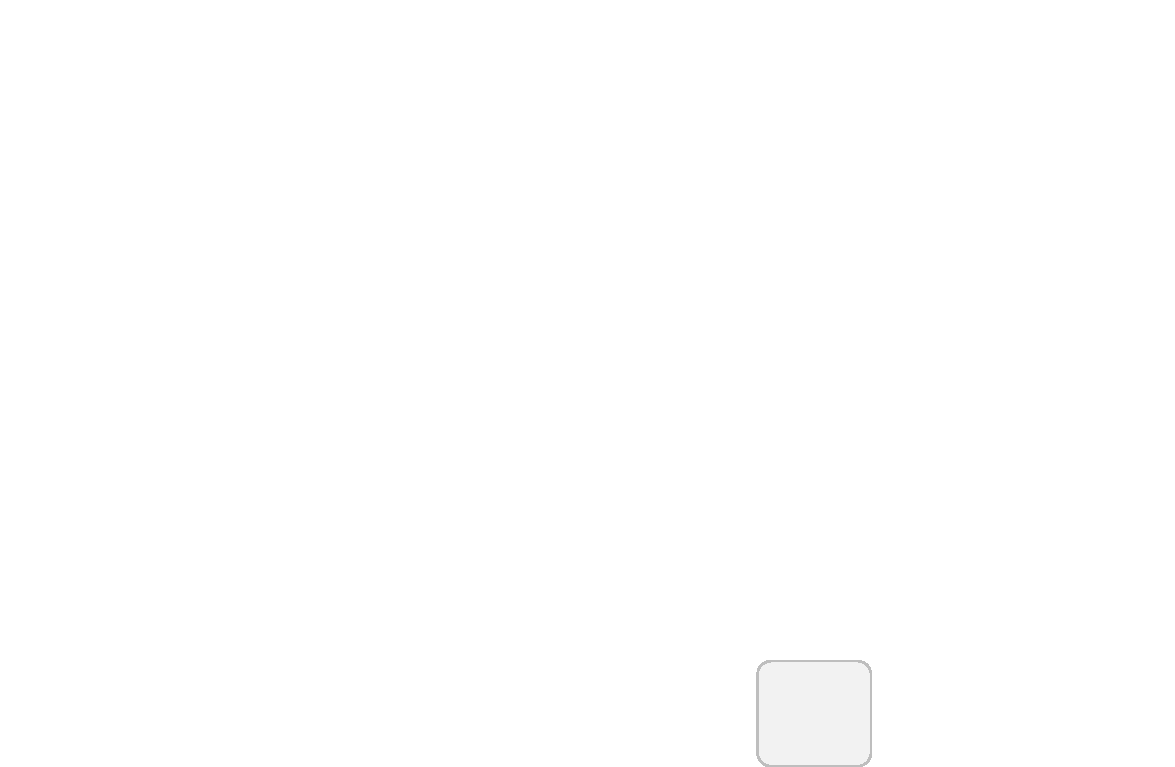
\includegraphics[width=\unitlength,page=1]{figures/reactors_wibench.pdf}}%
    \put(0.6526984,0.08228477){\color[rgb]{0,0,0}\makebox(0,0)[lb]{\smash{WiBench}}}%
    \put(0,0){\includegraphics[width=\unitlength,page=2]{figures/reactors_wibench.pdf}}%
    \put(0.01844314,0.6441587){\color[rgb]{0,0,0}\makebox(0,0)[lb]{\smash{GenerateInputs}}}%
    \put(0,0){\includegraphics[width=\unitlength,page=3]{figures/reactors_wibench.pdf}}%
    \put(0.00851222,0.51221933){\color[rgb]{0,0,0}\makebox(0,0)[lb]{\smash{(0, 1nsec)}}}%
    \put(0,0){\includegraphics[width=\unitlength,page=4]{figures/reactors_wibench.pdf}}%
    \put(0.13193937,0.55265236){\color[rgb]{0,0,0}\makebox(0,0)[lb]{\smash{\textbf{2}}}}%
    \put(0,0){\includegraphics[width=\unitlength,page=5]{figures/reactors_wibench.pdf}}%
    \put(0.13193937,0.60798177){\color[rgb]{0,0,0}\makebox(0,0)[lb]{\smash{\textbf{1}}}}%
    \put(0,0){\includegraphics[width=\unitlength,page=6]{figures/reactors_wibench.pdf}}%
    \put(0.23834209,0.58882928){\color[rgb]{0,0,0}\makebox(0,0)[lb]{\smash{Encoder}}}%
    \put(0,0){\includegraphics[width=\unitlength,page=7]{figures/reactors_wibench.pdf}}%
    \put(0.37892474,0.58882928){\color[rgb]{0,0,0}\makebox(0,0)[lb]{\smash{RateMatcher}}}%
    \put(0,0){\includegraphics[width=\unitlength,page=8]{figures/reactors_wibench.pdf}}%
    \put(0.55976562,0.58882928){\color[rgb]{0,0,0}\makebox(0,0)[lb]{\smash{Scrambler}}}%
    \put(0,0){\includegraphics[width=\unitlength,page=9]{figures/reactors_wibench.pdf}}%
    \put(0.71919299,0.58882928){\color[rgb]{0,0,0}\makebox(0,0)[lb]{\smash{Modulator}}}%
    \put(0,0){\includegraphics[width=\unitlength,page=10]{figures/reactors_wibench.pdf}}%
    \put(0.87927356,0.58845893){\color[rgb]{0,0,0}\makebox(0,0)[lb]{\smash{Precoder}}}%
    \put(0,0){\includegraphics[width=\unitlength,page=11]{figures/reactors_wibench.pdf}}%
    \put(0.04585149,0.41390658){\color[rgb]{0,0,0}\makebox(0,0)[lb]{\smash{SubCarrierMapper}}}%
    \put(0,0){\includegraphics[width=\unitlength,page=12]{figures/reactors_wibench.pdf}}%
    \put(0.26561509,0.41390658){\color[rgb]{0,0,0}\makebox(0,0)[lb]{\smash{SCFDMAModulator}}}%
    \put(0,0){\includegraphics[width=\unitlength,page=13]{figures/reactors_wibench.pdf}}%
    \put(0.5015007,0.41390658){\color[rgb]{0,0,0}\makebox(0,0)[lb]{\smash{ChannelReactor}}}%
    \put(0,0){\includegraphics[width=\unitlength,page=14]{figures/reactors_wibench.pdf}}%
    \put(0.70909382,0.41336561){\color[rgb]{0,0,0}\makebox(0,0)[lb]{\smash{SCFDMADemodulator}}}%
    \put(0,0){\includegraphics[width=\unitlength,page=15]{figures/reactors_wibench.pdf}}%
    \put(0.03746624,0.23781008){\color[rgb]{0,0,0}\makebox(0,0)[lb]{\smash{SubCarrierDemapper}}}%
    \put(0,0){\includegraphics[width=\unitlength,page=16]{figures/reactors_wibench.pdf}}%
    \put(0.28833335,0.23781008){\color[rgb]{0,0,0}\makebox(0,0)[lb]{\smash{EqualizerReactor}}}%
    \put(0,0){\includegraphics[width=\unitlength,page=17]{figures/reactors_wibench.pdf}}%
    \put(0.50868771,0.23781008){\color[rgb]{0,0,0}\makebox(0,0)[lb]{\smash{TransformDecoderReactor}}}%
    \put(0,0){\includegraphics[width=\unitlength,page=18]{figures/reactors_wibench.pdf}}%
    \put(0.80658014,0.23781008){\color[rgb]{0,0,0}\makebox(0,0)[lb]{\smash{Demodulator}}}%
    \put(0,0){\includegraphics[width=\unitlength,page=19]{figures/reactors_wibench.pdf}}%
    \put(0.03547694,0.08228477){\color[rgb]{0,0,0}\makebox(0,0)[lb]{\smash{Descrambler}}}%
    \put(0,0){\includegraphics[width=\unitlength,page=20]{figures/reactors_wibench.pdf}}%
    \put(0.23559506,0.08228477){\color[rgb]{0,0,0}\makebox(0,0)[lb]{\smash{RxRateMatcher}}}%
    \put(0,0){\includegraphics[width=\unitlength,page=21]{figures/reactors_wibench.pdf}}%
    \put(0.45130415,0.08228477){\color[rgb]{0,0,0}\makebox(0,0)[lb]{\smash{TurboDecoder}}}%
    \put(0,0){\includegraphics[width=\unitlength,page=22]{figures/reactors_wibench.pdf}}%
  \end{picture}%
\endgroup%
}
	%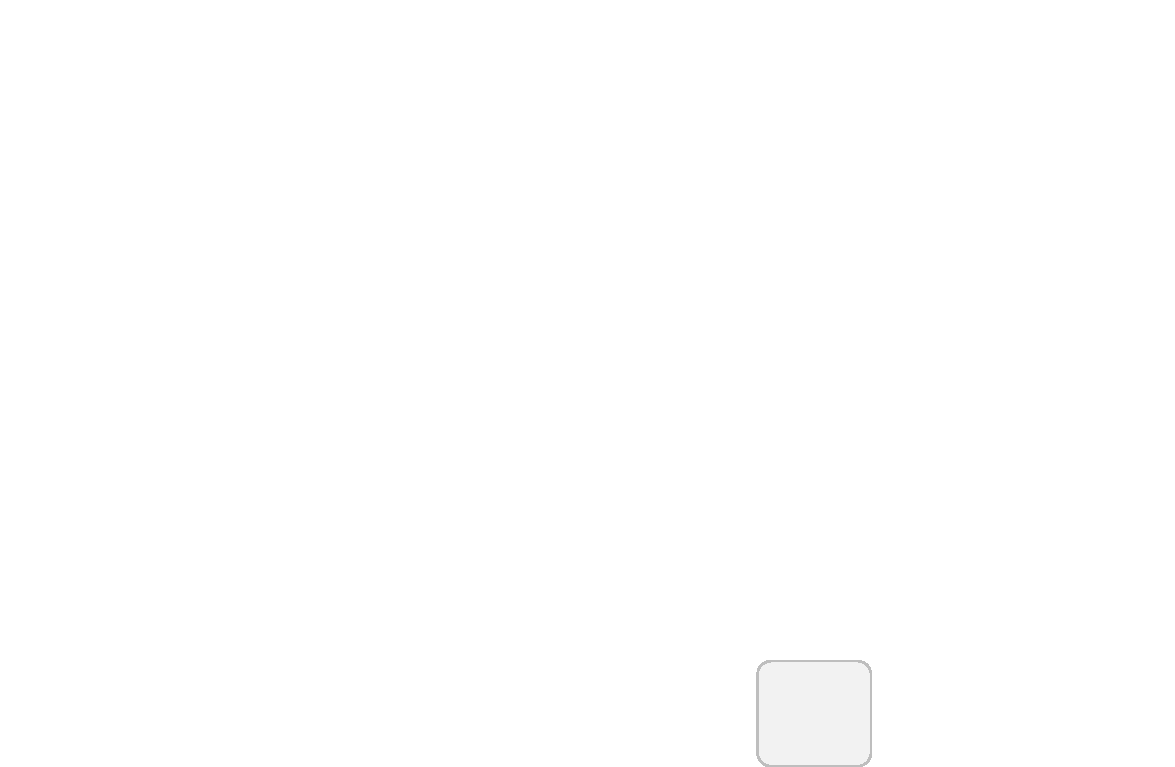
\includegraphics[width=0.46\textwidth]{figures/reactors_wibench.pdf}
	\caption{The Reactor network of the modified WiBench benchmark in Lingua Franca.}
	\label{fig:reactors_wibench}
\end{figure}


In ongoing (unpublished) work with Robert Wittig and Christian Menard, we adapted the WiBench benchmark~\cite{wibench} to work with Lingua Franca, an implementation of Reactors. 
Figure~\ref{fig:reactors_wibench} depicts the Reactor network implementing this benchmark. 
Since WiBench is single threaded, we only compared to a single threaded version in Reactors.
In particular, we did not leverage data level parallelism throughout the layer, nor the pipeline parallelism that we get from the network's topology for free.
This is a worst-case assumption we made to analyze the overhead.
By using the Reactor model, the benchmark is deterministic, even if it was to run using this parallelism~\cite{lohstroh_cyphy19}.
More importantly though, we can use the model's time semantics to define the constraints that ensure each subframe is processed on time.
Our implementation is thus still static (cf. Figure~\ref{fig:reactors_wibench}), since we have not yet specified well-defined mutations.
This implementation presents a great opportunity for future work to research and develop safe mutations for 5G.

Our implementation of the Reactor-based WiBench had an overhead of $15\%$ (median over $100$ executions), compared to the baseline implementation of WiBench.
There is certainly potential to improve this, e.g. as the scheduler of the C++ implementation on Lingua Franca, used for this implementation, was not optimized at all.
Nevertheless, this is a purely software-based implementation, so it serves only as a very rough estimation of the overhead; it is best suited to study the model's suitability and develop Reactor mutations for adaptability.
An efficient implementation in practice could work with reconfigurable hardware, e.g. implementing a \ac{PRET}~\cite{pret} machine, which is well-suited to Reactors' semantics.

In general, these preliminary results open up many avenues for research in adaptability in 5G. We can the Reactors model, at the semantic level to support the necessary adaptability in 5G. Similarly, we can design reconfigurable hardware that implements it.

\subsubsection{Other applications: Automotive}

The reactors model has many desirable properties for designing reliable \acp{CPS}, which can be applied in a multitude of domains.
An important example is the automotive domain, where the high-performance requirements of autonomous driving and modern entertainment are coupled with the timed \ac{CPS} including the car and its surroundings.
To keep the scope of this thesis limited, we omit a thorough discussion of an application of Reactors in the automotive domain.
In~\cite{menard_date20}, we showed how we can use the Reactors model to achieve determinism in the AUTOSAR \ac{AP}, a modern automotive standard.
 %ict + new

\chapter{Programming Languages}
\label{chap:pl}
In this thesis we have discussed multiple \acfp{MoC}, reasoning about their semantics and how to best deploy them on a particular hardware architecture.
A natural question arising from this is, ``how do we program in these \acp{MoC}?''.

In Chapter~\ref{chap:mapping}, Section~\ref{sec:kpn_basic} we saw the \acf{CPN} language.
\ac{CPN} is a \ac{DSL} designed to describe data flow programs with the Kahn-MacQueen blocking-read semantics, with special annotations for \ac{SDF} actors.
Other \ac{MoC}-based languages exist, like the CAL actor language~\cite{eker2003cal}, (TODO: the sesame description?) or Lingua Franca~\cite{lohstroh2020language}.
These languages allow ``freedom from choice''~\cite{lee2019freedom}, by enforcing a model that limits the ways in which to make mistakes, ideally without compromising the expressiveness of what can be designed with the model.

A common trade-off when designing programming languages is also the question of expressiveness versus performance.
High-level expressive abstractions are often at odds with low-level performance optimizations.
However, well-designed abstractions can be leveraged with semantics-preserving compiler transformations that still derive an efficient execution.
The whole principle of software synthesis can be seen as an instance of this principle.

This chapter discusses programing languages for defining and enforcing the semantics of a \ac{MoC}.
After a short review of existing languages, it focuses on the Ohua~\cite{ertel_phdthesis} language, which defines dataflow implicitly.
It also discusses how we can leverage the language and its semantics to define semantics-preservings transformations at a language level that can optimize the execution.
\section{Freedom from Choice}
In this Section we introduce the Ohua programing paradigm~\cite{ertel_phdthesis}.
The Ohua programming model by S. Ertel and others is a powerful model of implicit parallelism which can be used to express parallelism at a language level without explict costructions like threads and locks. 
This model is not part of the original contribution of this thesis. However, it is central to several distinct original contributions of the thesis, and we will introduce it as background material.

Ohua is best understood by diving directly into examples. Consider the code in Figure~\ref{fig:ohua_example}.
\begin{figure}[h]
	\centering
   \resizebox{0.55\textwidth}{!}{\begin{tikzpicture}
\draw (0,0) rectangle (5,5);
\draw (2.5,2.5) node {Placeholder};
\end{tikzpicture}
}
	\caption{A placeholder picture.}
	\label{fig:ohua_example}
\end{figure}

\todo{discuss example}.

The example in Figure~\ref{fig:ohua_example} can be transformed into a dataflow graph for execution. Figure~\ref{fig:ohua_example_df} depicts this example as a dataflow graph.
\todo{discuss dataflow graph}.

This duality between code and dataflow graphs is the core concept behind Ohua. More generally, Ohua defines a language...
\todo{discuss ohua formally}

\subsection{Stateful Functions}

\subsection{Dataflow Execution}

\subsection{$\lambda$-calculus-based Language}
 
\section{Stateful Parallelism}
Discuss idea behind~\cite{ertel_haskell19}, not implementation.

Also discuss formalization in Category Theory~\cite{ertel_haskellsup19}
\section{Concise code and Efficient \ac{I/O}}
Dataflow models expose concurrency. While concurrency enables parallelism, it can also be leveraged in other ways. 
This section discusses \"{Y}auhau, a framework for optimizing \ac{I/O} in microservice-based systems~\cite{ertel_cc18}.\index{\"{Y}auhau}
This Ohua-based framework uses the concurrency exposed by the \ac{MoC} to do so.

\begin{figure}[t]
        \centering
        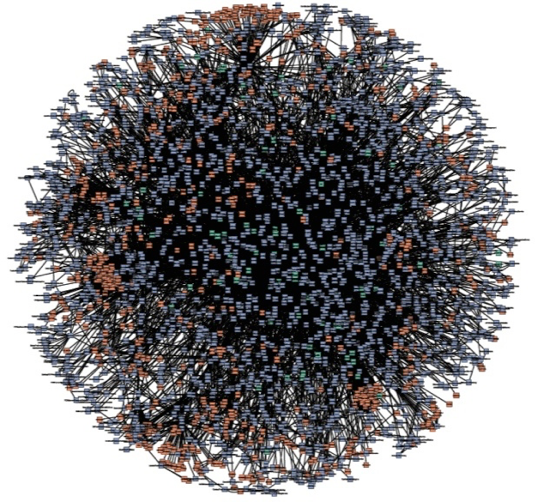
\includegraphics[scale=0.25]{figures/amazon-microservices.png}\\
        \small

        [Source: \href{https://www.slideshare.net/apigee/i-love-apis-2015-microservices-at-amazon-54487258}{I Love APIs 2015} by Chris Munns, licensed under \href{https://creativecommons.org/licenses/by/4.0/}{CC BY 4.0}, available at: \href{http://bit.ly/2zboHTK}{\url{http://bit.ly/2zboHTK}}]
        \vspace{-1mm}
        \caption{Microservices at Amazon.}
        \label{fig:amazon_death_star}
        \vspace{-3mm}
\end{figure}

The infrastructure of large internet companies today relies to a great extent on microservice-based architectures~\cite{decandia2007dynamo,marlow2014haxl}.
Figure~\ref{fig:amazon_death_star} shows the microservice infrastructure of Amazon circa 2015. 
It shows microservices as nodes, and how they depend on each other as edges.
The figure serves to illustrate the complexity of microservice-based architectures.

In microservice-based systems, \ac{I/O} plays a crucial role in the performance.
A microservice will commonly send multiple requests to a different microservice, as part of its operation.
Each request comes with a significant overhead from establishing the connection and sending the data.
If the requests do not depend on each other, however, they can instead be sent as a single, batched request for mitigating the overhead.

Batching requests is not a novel idea, it is well-established as a technique to optimize \ac{I/O}.
The trade-off comes from the code required to write batched requests.
A developer writing code for such a microservice-based architecture needs to take both the funcionality and the \ac{I/O} optimizations into account.
This makes the code harder to write, read and mantain, as the optimizations clutter the readability of the functionality.
This is unacceptable in a context where development time is a highly valuable resource, be it for human-resource costs or because it is important to have working solution as quick as possible. 

The suituation described is the case for Facebook's spam-fighting services~\cite{marlow2014haxl}.
When fighting spam, a novel filter must not only be effective and perform efficiently, it also should be implemented as fast as possible without compromising the functionality.
An ideal spam-fighting system thus allows the developers to focus on the functionality, and optimizes the implementation without cluttering the code.
This is precisely what the Haxl\index{Haxl} sytem attempts, using the Haskell abstraction of \emph{applicative functors}\index{applicative functor}.
Consider the Haskell code snippet (taken from \cite{marlow2014haxl}) in Listing~\ref{listing:haxl_friends_of}:

\begin{listing}[h]
\begin{minted}[]{Haskell}
let numCommonFriends =
     length (intersect (friendsOf x) (friendsOf y))
in
if numCommonFriends < 2 && daysRegistered x < 30
    then...
    else...
\end{minted}
\caption{An example of a Spam-fighting request to be optimized by Haxl (from ~\cite{marlow2014haxl}).}
\label{listing:haxl_friends_of}
\end{listing}

The listing shows a code example where, for spam fighting, the number of common Facebook friends of two users are calculated.
This is done by calling the function \texttt{friendsOf} for both \texttt{x} and \texttt{y}.
Code like Listing~\ref{listing:haxl_friends_of} is easy to read, but unoptimized, it will send to requests to the microservice that handles the \texttt{friendsOf} function.
The solution of Haxl is to use applicative functors to compose \ac{I/O} calls, such as \texttt{friendsOf}, and automatically batch independent requests this way.
Listing~\ref{listing:haxl_appliactive_do} shows how this is achieved in Haxl using applicative-do notation.

\begin{listing}
\begin{minted}[]{Haskell}
do a <- friendsOf x
   b <- friendsOf y
   return (length (intersect a b))
\end{minted}
\caption{The request from Listing~\ref{listing:haxl_friends_of} batched using applicative-do (from ~\cite{marlow2014haxl}).}
\label{listing:haxl_applicative_do}
\end{listing}

Under the hood, the applicative functor definition for \texttt{friendsOf} in Haxl gathers the arguments \texttt{x} and \texttt{y} and makes a single, batched request.
This optimizes the execution with a minimal obfuscation of the code:
A developer has to switch from a pure functional style to an applicative style, but can otherwise focus on the semantics of the program.

Our central observation is that this \ac{I/O} optimizations all come ``for free'' from the exposed concurrency in a dataflow execution. 
If we define a dataflow operator that gathers the inputs and issues a single batched request, we get the composition from the semantics of dataflow.
This is the main idea behind \"{Y}auhau.


\"{Y}auhau is based on the iteration of Ohua embedded in Clojure.
It is a language with an explicit annotation for functions which perform \ac{I/O}.
Leveraging these annotations, a semantics-preservig transformation can minimize the number of independent \ac{I/O}-performing function calls.
We map the Clojure-based Ohua to an internal expression \acsu{IR}, as is shown in Figure~\ref{fig:clojure_to_yauhau}.

\begin{figure}[h]
	\centering
	\begin{tabular}{r r c l r r r c l r}
		&\mintinline{Clojure}{x} & $\mapsto$ & $x$ &  &\mintinline{Clojure}{(let [x t] t)} & $\mapsto$ & $\lit*{let} \: x = t \: \lit*{in} \: t$ &  \\

	&\mintinline{Clojure}{(io x)}&$\mapsto$& $\lit*{io}(x)$ & &\mintinline{Clojure}{(fun [x] t)} $\equiv$ \mintinline{Clojure}{#(t)} & $\mapsto$ & $\lambda x.t$ &\\ 
	&\mintinline{Clojure}{(t t)} & $\mapsto$ & $t \: t$ &	 &\mintinline{Clojure}{(f x1 ... xn)} & $\mapsto$ & $\lit*{ff}_f(x_1 \ldots x_n)$ & \\
    & & & & &	\mintinline{Clojure}{(if t t t)} & $\mapsto$ & $\lit*{if}(t \: t \: t)$  	%		\\
		%		\multicolumn{4}{l}{\textit{Values:}}\\
		%		&\mintinline{Clojure}{(reqF x1 ... xn)}& $\mapsto$ & $r_f$ & \\
	\end{tabular}
	
	\caption{Mapping the terms of the Clojure-based language to an expression \acs{IR}. Adapted from Figure~9 in~\cite{ertel_cc18}.}
	\label{fig:clojure_to_yauau}
\end{figure}

The expression \ac{IR} defined in Figure~\ref{fig:clojure_to_yauau} is based on $\lambda$ calculus with a \texttt{let} construction for lexical scoping and explicit conditionals (\texttt{if}).
The central innovations of the language are the two particular terms, \texttt{ff} for foreign functions, which is any (possibly stateful) function.
The other term is \texttt{io}, which is an explicit annotation that a function does \ac{I/O}\index{\"{Y}auhau ! io}.
The premise is to optimize the number of annotated \ac{I/O} calls leveraging the concurrency from the dataflow semantics derived from this language.
The example in Listing~\ref{listing:yauhau_friends_of} lists the same request as Listing~\ref{listing:haxl_friends_of} in \"{Y}auhau.

\begin{listing}
\begin{flalign*}
& \lit*{let}~\lit*{numCommonFriends} = & \\ 
& \quad \lit*{ff}_\text{length}(\lit*{ff}_\text{intersect}( & \\ 
& \quad \quad \lit*{ff}_\text{friendsOf}(\lit*{io}(x)),~\lit*{ff}_\text{friendsOf}(\lit*{io}(y)) & \\
& \quad ))~\lit*{in}~\ldots & 
\end{flalign*}
\caption{The request from Listing~\ref{listing:haxl_friends_of} in \"{Y}auhau.}
\label{listing:yauhau_friends_of}
\end{listing}

The \ac{I/O} optimizations in \"{Y}auhau come from batching requests.
Instead of calling \texttt{ff}$_\text{friendsOf}$(\texttt{io}(\texttt{x})) and \texttt{ff}$_\text{friendsOf}$(\texttt{io}(\texttt{y})) as two separate \ac{I/O} requests, we can call them as a single batched request, since they are independent.
In \"{Y}auhau we do so by introducing a \emph{batched} \ac{I/O} statement, \texttt{bio}\index{batched \acs{I/O}}.
The \texttt{bio} statement takes a list of arguments and does a batched call with this list.
In the example, the two statements become a single \texttt{ff}$_\text{friendsOf}$(\texttt{bio}(\texttt{[x,y]}).

Through semantics-preserving transformations using \texttt{let} floating we can get independent \ac{I/O} calls batched this way and transform them to dataflow.
The explicit concurrency in the dataflow transformation allows to execute batched \ac{I/O} calls when they arrive.
An important advantage of this is that it also allows us to transcend the function boundaries
 %cc_18


\chapter{Related Work}
Discuss related work.


\chapter{Conclusions} 
Programming computers is notoriously difficult.
This thesis certainly will not change that, and more generally, this statement will probably remain true for a long time.
This does not mean, however, that we cannot make progress towards easing the process of programming computers.

In this thesis we have argued for model-based design of software systems.
This is much more common in the hardware world, where models are central to design and deterministic behavior.
The success of this paradigm is what allows us to have programmable digital computers in the first place.

In the software world, where the level of abstraction is higher and the barrier to entry lower, models are usually more implicit, less strict, or both.
When using well-defined \acfp{MoC} for programming, however, we can reason about software and its performance.
Concretely, software synthesis flows and the mapping problem result from doing precisely this.

In this thesis we studied such \ac{MoC}-based software synthesis flows, with a focus on \acf{KPN}.
We surveyed multiple dataflow \acp{MoC}, and discussed the advantages and disadvantages of them. 
The \ac{KPN} \ac{MoC} allows us to express concurrency in computation in a deterministic fashion, while remaining very expressive.
Compared to most dataflow \acp{MoC}, it allows for maximally dynamic, data-dependent behavior.
We also discussed a semantics gap between the \acfp{KMQ} blocking-reads semantics and \ac{KPN}, which can be exploited in applications with data-parallelism.

When lowering \acp{KPN} down to be executed in \acp{MPSoC}, the mapping problem plays a crucial role, especially for heterogeneous systems.
In this thesis we have discussed this intractable problem at length.
A central theme of our discussion has been the structure of the mapping space.
We have seen how the space is large and complex, yet structured.

The mapping space is very symmetrical, which concretely means that many mappings are equivalent in terms of properties like performance or energy efficiency.
This is due to symmetries in the target hardware architectures and applications.
\acp{MPSoC} usually have multiple cores with identical microarchitectures and memory subsystems with a regular structure.
Data-level parallelism in applications also yield such symmetry.
We have seen how to describe and exploit this symmetry, pruning the mapping space for \acf{DSE} or for finding equivalent mappings when some resources are unavailable at run-time.

The mapping space also has different geometric interpretations.
We have seen how to find different embeddings of these geometric interpretations and exploit them in \ac{DSE} meta-heuristics.
This also allowed us to design novel heuristics and meta-heuristics, based on the geometric structure of the space, to find mappings with low communication costs or high robustness.
In general, we have seen how the way we represent mappings can expose much of this structure.
We believe much work would benefit from explicitly considering the structure exposed to the algorithms.

There is little point in exposing complex structures and engineering sophisticated algorithms if they don't improve our methods.
To assess if they do, however, we need to test them, using benchmarks.
Given the importance of this, we argue for careful consideration as to what and how improvements are assessed using benchmarks.
In this thesis we have argued for a statistical view of code, seeing improvements on methods as improvements on the expected value of some property, like the program's execution time.

Unfortunately, benchmarks are scarce and seldom specialized.
We have discussed options for is overcoming this issue, using random benchmark generation and machine learning.
In particular, we have seen how our statistical view of code for benchmarking exposes some possible pitfalls of machine learning for benchmark generation, both in theory and in practice.

While \ac{KPN}-based flows have many advantages, they are not well-suited for every application domain.
For example, \acp{KPN} do not have semantics to deal with time, which is important in \acfp{CPS}.
Similarly, the \ac{KPN} graph structure is rigid, which limits the adaptability of the model.
In this thesis we discussed a novel model, Reactors, which addresses these limitations.
We focused on the opportunities of this model in the 5G telecommunications standard. 

Most of this thesis has focused on the advantages of model-based design, which are plentiful. 
An important disadvantage, however, is the ease of use of this design process.
Exposing models through \acp{API} is not productive, since developers can and usually do end up abandoning the model's constraints.
We need programming languages and, especially, programming models that make \ac{MoC}-based design accessible to programmers, while enforcing the model's constraints.
In this thesis we briefly discussed the Ohua programming model, which derives a dataflow execution implicitly from a conventional programming language. 
We saw how we can use this to combine the advantages of \ac{MoC}-based design with concise programming, by optimizing \acs{I/O} in microservice-based infrastructures.

\section{Future Work}

We believe the single most important aspect to drive \ac{MoC}-based design forward is fostering its adoption.
We need tools and environments that make it easier for programmers to design applications with a well specified \ac{MoC}.

The Lingua Franca project, which implements Reactors, is a great avenue for fostering adoption.
Its polyglot design allows programmers to use known languages to write reactors, while still being a coordination language that can enforce the \ac{MoC} semantics.
The use of known language has two distinct advantages, as it reduces the learning curve and allows to use legacy code. 
Currently, the compiler does not understand nor type-check the target language, leaving that task to the compiler.
In future work we could add a type system to Lingua Franca, reinfoncing the ``freedom from choice'' it provides.

A potential disadvantage from the Lingua Franca project, on the other hand, could be its coordination language. 
Explicitly writing the networks can be confusing for developers.
This is exacerbated by the fact that Reactors is a complex model, difficult to grasp and learn.
We believe the approach by Ohua of making the network implicit is a great avenue for future work.
Another example to follow is the Elm language, a functional language for the web.
Elm started as a language with an explicit \ac{FRP} paradigm, which was confusing for users.
They made this paradigm implicit~\footnote{\url{https://elm-lang.org/news/farewell-to-frp}}, which translated into a success for the learning curve and the language's adoption.
This is part of a general vision, where compilers and languages are thought of as assistants that make development easier for programmers, instead of only focussing on correctness and performance.
We believe we should follow similar paths for the design of software using \acp{MoC} like Reactors or \ac{KPN}.

On the side of mapping there are also many open avenues for improving our work.
In particular, partial symmetries expose a great deal of the problem's structure which we are not exposing yet.
Designing efficient methods to detect and exploit them would help navigate the design space of mappings much better.
This would also open up opportunities for using inverse semigroups of non-symmetries, like reducing the number of hops in a communication link.
Our methods would also greatly benefit from incorporating application symmetries when exploting data-level parallelism.  

The geometry of the mapping space also has many open questions that should improve its usefulness.
While we discussed the trade-off between the distortion and dimensionality of embeddings, we did not exploit it in this thesis.
More importantly, while the metrics we discussed are a good starting point, we saw that they do not reflect the mapping structure very well yet.
Finding better metrics could greatly improve mapping meta-heuristics, especially those based on some concept of locality in the search space.

In this thesis we have discussed and shown how provable properties of \acp{MoC} can and do improve the design process.
While traditional pen and paper proofs are a great way of finding and proving these properties, the advent of powerful theorem proving assistants provides an opportunity to improve upon this.
Formally verified proofs of properties of the system give us more certainty on their correctness, and some degree of automation.
Combining \ac{MoC}-based design with developments in formal verification methods can help us to write correct software more frequently and with less time.

While formal methods can verify properties of our software, they might never completely replace testing.
Even if they one day do so, that will not be in the near future.
This is why we believe the work on benchmarking is an important avenue for future work.
We believe advances in machine learning could enable our vision of benchmark generation flows.
Informed by statistical models and tailored for a specific use-cases, such benchmark generation flows could dramatically change the way we assess our compilers.


\appendix

\chapter{Groups and Inverse Semigroups}
\label{appendix:groups}
Group theory and inverse semigroups

\chapter{Metric Spaces and Low-Distortion Embeddings}
\label{appendix:metric}
Here we discuss (discrete) metric spaces and low-distortion embeddings.
A metric space is the mathematical formalization of distances. 
We define a metric to be able to measure distances in a particular space. 

\begin{defn}
Let $M$ be a set and let $d : M \times M \rightarrow \mathbb{R}_{\geq 0}$ .
We say that $d$ is a metric on $M$ and, equivalently, $(M,d)$ is a metric space, if the following hold:
\begin{enumerate}
\item\label{ax:zero} For all $m,m' \in M, d(m,m') = 0 \Leftrightarrow m = m'$.
\item\label{ax:symm} For all $m,m' \in M$, we have $d(m,m') = d(m',m)$.
\item\label{ax:triangle} For all $k,l,m \in M$ we have $d(k,m) \leq d(k,l) + d(l,m)$
\end{enumerate}
\end{defn}

The motivation for these properties is intuitively clear.
Property~\ref{ax:zero} says two things, first, that there is no distance from an element to itself, and second, that no two equal elements are in the same place (have no distance between them).
If we don't require the second property (i.e. replace $\Leftrightarrow$ with $\Rightarrow$ in Property~\ref{ax:zero}, we get what is called a pseudo-metric (or a degenerate metric).
The second property, Property~\ref{ax:symm} states that distance is symmetric.
Finally, Property~\ref{ax:triangle} is the triangle inequality: it states that the shortest path between two elements is always the direct path, their distance.

The canonical metric spaces are $\mathbb{R}^n$ with different norms, like the $p$-norms.
A norm is a more restrictive concept than a metric, but we will not define norms here further.
\begin{ex}
    For $p \geq 1$, the function $(x,y) \mapsto \| x -y \|_p : \mathbb{R}^n \times \mathbb{R}^n \rightarrow \mathbb{R}_{\geq 0}$ is a metric, where 
    $\| (x_1,\ldots,x_n) \|_p := (\sum_{i=1}^n|x_i^p|)^{1/p}$ is the $p$-norm.
\end{ex}

The case for $p = 2$ is the well-known Euclidean distance in vector spaces.
Also well-known is the case of of $p=1$, which is sometimes called the Mahattan or Taxi distance, in allusion to the distance when moving through the streets of a neighborhood that look like a regular mesh, like in Manhattan.

In this thesis we are particularly interested in the case where $M$ is finite, which we will assume from here on. 
If $M = \{ m_1, \ldots, m_n \}$ is finite, we can write $d$ as a matrix, such that $d(m_i,m_j) = D_{i,j}$.:
\begin{equation*}
    D = 
\left(
\begin{array}{cccc}
d(m_1,m_1) & d(m_1,m_2) & \ldots & d(m_1,m_n) \\
d(m_2,m_1) & d(m_2,m_2) & \ldots & d(m_2,m_n) \\
\vdots & \vdots & \ddots & \vdots \\
d(m_n,m_1) & d(m_n,m_2) & \ldots & d(m_n,m_n) \\
\end{array}
\right)
\end{equation*}

The structure preserving mappings (moprhisms) of metric spaces are called \emph{isometries}\index{isometry}. They have the particular property that they are always injective, due to Property~\ref{ax:zero}.
\begin{defn}
Let $M,M'$ be metric spaces. We say that a mapping $\varphi : M \rightarrow M'$ is an \emph{isometry} if for all $m,m' \in M$, $d_M(m,m') = d_{M'}(\varphi(m),\varphi(m'))$.
\end{defn}
An isometry is thus always an embedding (monic), since for any two points $m,m' \in M$ with $\varphi(m) = \varphi(m')$ we have $0 = d_{M'}(\varphi(m),\varphi(m')) = d_{M}(m,m')$.

In the case of groups, embeddings into a particular group $S_n$ are useful for computing.
While we did not discuss it as thoroughly, the basis of all computation we are concerned with in this thesis are these embeddings into permutation groups 
$S_n$\footnote{In computational group theory there are other branches like matrix groups or black-box groups, where embedding into an $S_n$ is infeasible,
but we are not concerned with these in this thesis.}.
The question is, can we find an equivalent method for metric spaces, using isometries to (finite subsets of) $\mathbb{R}^n$? 
The unfortunate answer is that no, for a finite metric space $M$ there is not always $n,p$ such that there exists an isometry from $M$ to $(\mathbb{R}^n,\|\cdot\|_p)$ (see~\cite{matouvsek} for a proof).
Fortunately, however, when dealing with real numbers we can always look for approximations.

\begin{defn}
Let $M$ be a metric space and $\iota: M \hookrightarrow \mathbb{R}^n$ be an embedding onto $\mathbb{R}^n$. 
We say that $\iota$ has distortion $D > 0$ if 
\begin{align*} \frac{1}{D} d(x,y) \leq \| \iota(x) - \iota(y) \| \leq d(x,y) \end{align*}
\end{defn}

While, in general, we cannot find an isometry, we can search for an embedding with a low distortion.
There is a particularly useful result in this context:
we can use convex optimization to find an embedding of $M$ onto $\mathbb{R}^n$ with the Euclidean ($p=2$) norm~\cite{matouvsek}.
This is unfortunately only the case for this norm, e.g. for $p=1$ finding such an embedding is known to be NP-complete~\cite{matouvsek}

A problem with the convex optimization method above is that it yields an embedding with dimension $|M|$, which might be very high.
The dimension of the vector space strongly affects algorithmic properties of the problem. 
It would be ideal to find an embedding into a mapping with a lower dimension, without increasing the distortion much.
In~\cite{johnson_lindenstrauss}, Johnson and Lindenstrauss describe this precise problem and its solution as follows: 
``Given $n$ points in Euclidean space, what is the smallest $k = k(n)$ so that these points can be moved into $k$-dimensional Euclidean space via a transformation that expands or contracts all paairwise distances by a factor of at most $1 + \epsilon$? The answer, that $k \leq c(\epsilon) \operatorname{Log} n$, is a simple consequence of the isoperimetric inequality for the $n$-sphere studied in~\cite{figiel1977dimension}.''
They proceed to formalize and prove this fact, which we will not restate here more precisely.
This  result is known as the Johnson-Lindenstrauss Lemma. \index{Johnson-Lindenstrauss lemma}

An intuitive albeit sometimes misleading interpretation of the proof of this lemma is that a projection onto a \textbf{random} subspace will have a low distortion with high probability.
In practice, the distribution does give a very useful ``transform'' for dimensionality reduction, simply by projecting onto a random subspace.
However, we should be careful when using this and ideally check the distortion, if possible.
%\chapter{Denotational Semantics}
%\label{appendix:semantics}
%Denotational semantics.


%\bibliographystyle{alpha}
%\bibliography{aux/references,aux/mios}
\clearpage
\printbibliography[title={References},notkeyword={contribution}]

\listoffigures

\printindex

\chapter*{List of Acronyms}
%https://tex.stackexchange.com/questions/38558/how-to-pluralize-an-acronym-which-ends-in-s-correctly#38559
\begin{acronym}
  \acro{ALU}{Arithmetic Logic Unit}
  \acro{ANOVA}{Analysis of Variance}
  \acro{AP}{Adaptive Platform}
  \acro{API}{Application Programming Interface}
  \acro{AST}{abstract syntax tree}
  \acro{BNF}{Backus-Naur Form}
  \acro{BSGS}{base and strong generating set}
  \acro{CDFG}{control- and data-flow graph}
  \acro{cfaed}{Center for Advancing Electronics Dresden}
  \acro{CAS}{computer algebra system}
  \acro{CFS}{Completely Fair Scheduler}
  \acro{CGO}{International Symposium on Code Generation and Optimization}
  \acro{CPN}{C for Process Networks}
  \acro{CPU}{Central Processing Unit}
  \acro{CPS}{Cyber-Physical System}
  \acro{CSDF}{Cyclo-Static Data Flow}
  \acro{CSP}{Communicating Sequential Process}
  \acroplural{CSP}[CSPs]{Communicating Sequential Processes}
  \acro{DDF}{Dynamic Data Flow}
  \acro{DLP}{data-level parallelism}
  \acro{DMA}{Direct Memory Access}
  \acro{DPN}{Dataflow Process Networks}
  \acro{DOL}{Distributed Operation Layer}
  \acro{DSE}{Design-Space Exploration}
  \acro{DSL}{Domain-Specific Language}
  \acro{HAEC}{Highly-Adaptive Energy-Efficient Computing}
  \acro{E3S}{Embedded System Synthesis Benchmarks Suite}
  \acro{EDA}{Electronic Design Automation}
  \acro{FFT}{Fast Fourier Transform}
  \acro{FIFO}{first in - first out}
  \acro{FPGA}{Field Programmable Gate Array}
  \acro{GAP}{Groups Algorithms Programming}
  \acro{GBM}{Group Based Mapping}
  \acro{GGNN}{Gated Graph Sequence Neural Network}
  \acro{GPU}{Graphics Processing Unit}
  \acro{GSM}{Global System for Mobile Communications}
  \acro{HLS}{High-Level Synthesis}
  \acro{HOG}{Histogram of Oriented Gradients}
  \acro{HSDF}{Homogeneous \ac{SDF}}
  \acro{IDE}{Integrated Development Environment}
  \acro{IFFT}{inverse \ac{FFT}}
  \acro{i.i.d.}{independent and identically distributed}
  \acro{ILP}{integer linear programming}
  \acro{IoT}{Internet of Things}
  \acro{IP}{intellectual property}
  \acro{IR}{intermediate representation}
  \acro{ISA}{Instruction-Set Architecture}
  \acro{I/O}{Input/Output}
  \acro{KPN}{Kahn Process Network}
  \acro{KMQ}{Kahn-MacQueen}
  \acro{LSTM}{Long Short-Term Memory}
  \acro{LTE}{Long Term Evolution}
  \acro{NoC}{Network on Chip}
  \acro{NVM}{non-volatile memory}
  \acroplural{NVM}[NVMs]{non-volatile memories}
  \acro{MAPS}{\ac{MPSoC} Application Programming Studio}
  \acro{MoC}{Model of Computation}
  \acroplural{MoC}[MoCs]{Models of Computation}
  \acro{MPSoC}{Multi-Processor System-on-Chip}
  \acroplural{MPSoC}[MPSoCs]{Multi-Processor Systems-on-Chip}
  \acro{OOP}{object-oriented programming}
  \acro{OS}{operating system}
  \acro{PCB}{printed circuit board}
  \acro{pdf}{probability density function}
  \acro{PACT}{International Conference on Parallel Architectures and Compilation Techniques}
  \acro{PE}{processing element}
  \acro{poset}{partially-ordered set}
  \acro{pthread}{POSIX thread}
  \acro{RTM}{race-track memory}
  \acroplural{RTM}[RTMs]{racetrack memories}
  \acro{RVC}{Reconfigurable Video Coding}
  \acro{SADF}{Scenario-Aware Data Flow}
  \acro{s.c.c.}{strongly connected component}
  \acro{SDF}{Synchronous Data Flow}
  \acro{\SDFFF}{\ac{SDF} For Free}
  \acro{TETRiS}{Transitive Efficient Template Run-time System}
  \acro{TGFF}{task graph for free}
  \acro{XML}{Extensible Markup Language}
\end{acronym}

\clearpage


\end{document}